\begin {figure}[h]
	\centering
		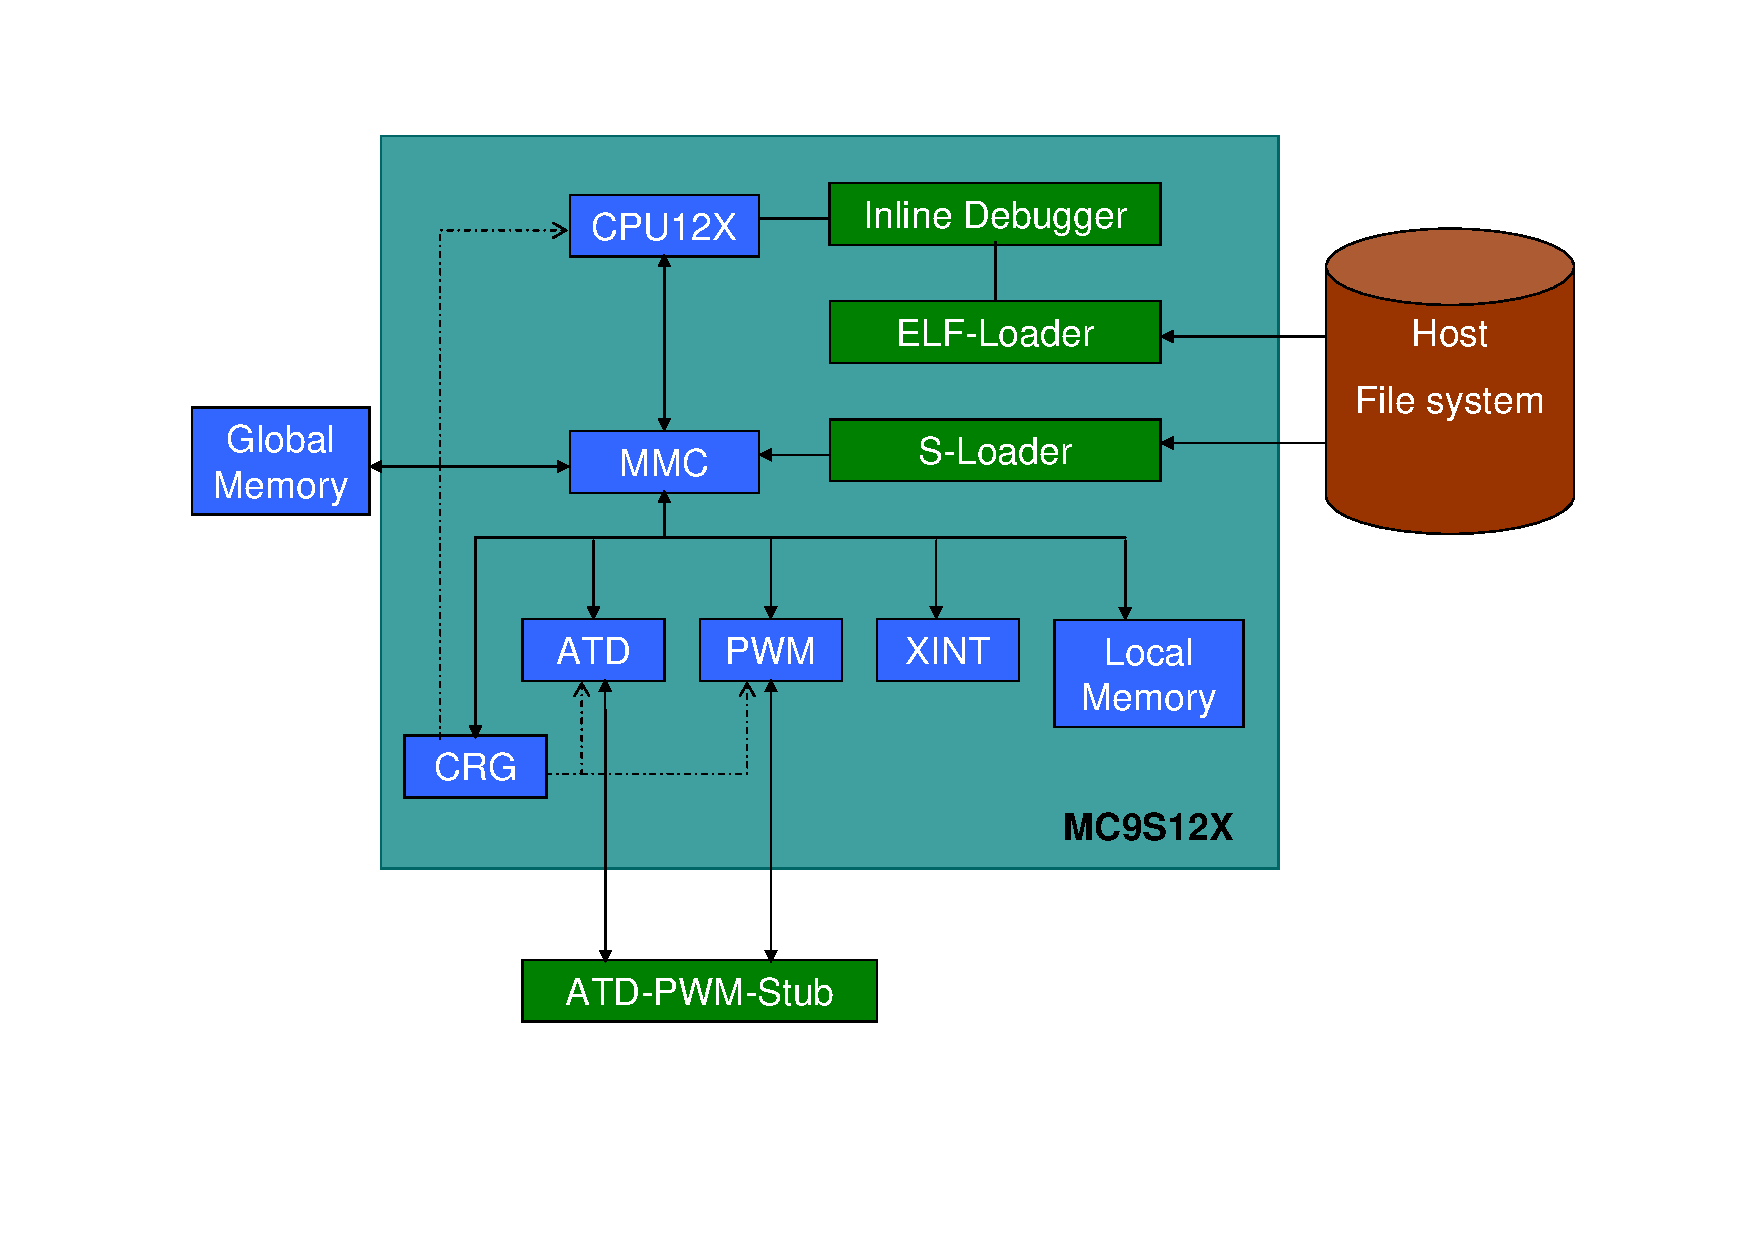
\includegraphics[width=1\textwidth]{mc9s12xdp512/mc9s12xdp512_schema.pdf}
	\caption {mc9s12x configuration.}
	\label {fig:mc9s12xdp512}
\end {figure}

\section{Introduction}
UNISIM star12x, a Star12X System-on-Chip simulator with support of ELF32 binaries and s19 hex files, and targeted for automotive applications
\section{Licensing}
UNISIM star12x 1.0\\
Copyright (C) 2008-2010, Commissariat a l'Energie Atomique (CEA)\\
License: BSD (see file COPYING)\\
Authors: Reda Nouacer $<$reda.nouacer@cea.fr$>$\\
\section{Simulated configuration}
\noindent The simulator is composed of the following modules and services:
\begin{itemize}\addtolength{\itemsep}{-0.40\baselineskip}
\item ATD0
\item ATD1
\item CPU
\item CRG
\item ECT
\item MMC
\item PWM
\item XINT
\item elf32-loader: ELF Loader
\item external-memory
\item external\_router
\item gdb-server: GDB Server
\item host-time: Host time
\item inline-debugger: Inline debugger
\item internal-memory
\item internal\_router
\item kernel\_logger: UNISIM kernel logger
\item memoryImportExportTee
\item registersTee
\item time: SystemC time
\item xml-atd-pwm-stub
\end{itemize}
\section{Using UNISIM star12x}
\noindent Usage: \texttt{unisim-star12x-1.0 [<options>] [...]}

\noindent Options:
\begin{itemize}
\item \texttt{--set $<$param=value$>$ or -s $<$param=value$>$}: set value of parameter 'param' to 'value'
\item \texttt{--config $<$XML file$>$ or -c $<$XML file$>$}: configures the simulator with the given XML configuration file
\item \texttt{--get-config $<$XML file$>$ or -g $<$XML file$>$}: get the simulator configuration XML file (you can use it to create your own configuration. This option can be combined with -c to get a new configuration file with existing variables from another file
\item \texttt{--list or -l}: lists all available parameters, their type, and their current value
\item \texttt{--warn or -w}: enable printing of kernel warnings
\item \texttt{--doc $<$Latex file$>$ or -d $<$Latex file$>$}: enable printing a latex documentation
\item \texttt{--version or -v}: displays the program version information
\item \texttt{--help or -h}: displays this help
\end{itemize}
\section{Configuration}
\tablehead{\hline}
\tabletail{\hline}
\begin{supertabular}{|p{7.5cm}|p{7.5cm}|}
\hline
\multicolumn{2}{|l|}{\textbf{\Large ATD0}}\\
\hline
\multicolumn{1}{|p{7.5cm}}{\textbf{Name:} \texttt{ATD0.bus-cycle-time}} & \multicolumn{1}{p{7.5cm}|}{\textbf{Type:} \texttt{64-bit floating-point}}\\
\multicolumn{1}{|p{7.5cm}}{\textbf{Default:} \texttt{250000}} & \multicolumn{1}{p{7.5cm}|}{}\\
\multicolumn{2}{|l|}{}\\
\multicolumn{2}{|p{15cm}|}{\textbf{Description:} \newline .}\\
\hline
\multicolumn{1}{|p{7.5cm}}{\textbf{Name:} \texttt{ATD0.base-address}} & \multicolumn{1}{p{7.5cm}|}{\textbf{Type:} \texttt{unsigned 16-bit integer}}\\
\multicolumn{1}{|p{7.5cm}}{\textbf{Default:} \texttt{0x2c0}} & \multicolumn{1}{p{7.5cm}|}{}\\
\multicolumn{2}{|l|}{}\\
\multicolumn{2}{|p{15cm}|}{\textbf{Description:} \newline .}\\
\hline
\multicolumn{1}{|p{7.5cm}}{\textbf{Name:} \texttt{ATD0.interrupt-offset}} & \multicolumn{1}{p{7.5cm}|}{\textbf{Type:} \texttt{unsigned 8-bit integer}}\\
\multicolumn{1}{|p{7.5cm}}{\textbf{Default:} \texttt{0xd2}} & \multicolumn{1}{p{7.5cm}|}{}\\
\multicolumn{2}{|l|}{}\\
\multicolumn{2}{|p{15cm}|}{\textbf{Description:} \newline .}\\
\hline
\multicolumn{1}{|p{7.5cm}}{\textbf{Name:} \texttt{ATD0.vrl}} & \multicolumn{1}{p{7.5cm}|}{\textbf{Type:} \texttt{64-bit floating-point}}\\
\multicolumn{1}{|p{7.5cm}}{\textbf{Default:} \texttt{0}} & \multicolumn{1}{p{7.5cm}|}{}\\
\multicolumn{2}{|l|}{}\\
\multicolumn{2}{|p{15cm}|}{\textbf{Description:} \newline .}\\
\hline
\multicolumn{1}{|p{7.5cm}}{\textbf{Name:} \texttt{ATD0.vrh}} & \multicolumn{1}{p{7.5cm}|}{\textbf{Type:} \texttt{64-bit floating-point}}\\
\multicolumn{1}{|p{7.5cm}}{\textbf{Default:} \texttt{5.12}} & \multicolumn{1}{p{7.5cm}|}{}\\
\multicolumn{2}{|l|}{}\\
\multicolumn{2}{|p{15cm}|}{\textbf{Description:} \newline .}\\
\hline
\multicolumn{1}{|p{7.5cm}}{\textbf{Name:} \texttt{ATD0.debug-enabled}} & \multicolumn{1}{p{7.5cm}|}{\textbf{Type:} \texttt{boolean}}\\
\multicolumn{1}{|p{7.5cm}}{\textbf{Default:} \texttt{false}} & \multicolumn{1}{p{7.5cm}|}{\textbf{Valid:} \texttt{true},~\texttt{false}}\\
\multicolumn{2}{|l|}{}\\
\multicolumn{2}{|p{15cm}|}{\textbf{Description:} \newline .}\\
\hline
\multicolumn{1}{|p{7.5cm}}{\textbf{Name:} \texttt{ATD0.vih}} & \multicolumn{1}{p{7.5cm}|}{\textbf{Type:} \texttt{64-bit floating-point}}\\
\multicolumn{1}{|p{7.5cm}}{\textbf{Default:} \texttt{3.25}} & \multicolumn{1}{p{7.5cm}|}{}\\
\multicolumn{2}{|l|}{}\\
\multicolumn{2}{|p{15cm}|}{\textbf{Description:} \newline .}\\
\hline
\multicolumn{1}{|p{7.5cm}}{\textbf{Name:} \texttt{ATD0.vil}} & \multicolumn{1}{p{7.5cm}|}{\textbf{Type:} \texttt{64-bit floating-point}}\\
\multicolumn{1}{|p{7.5cm}}{\textbf{Default:} \texttt{1.75}} & \multicolumn{1}{p{7.5cm}|}{}\\
\multicolumn{2}{|l|}{}\\
\multicolumn{2}{|p{15cm}|}{\textbf{Description:} \newline .}\\
\hline
\multicolumn{1}{|p{7.5cm}}{\textbf{Name:} \texttt{ATD0.Has-External-Trigger}} & \multicolumn{1}{p{7.5cm}|}{\textbf{Type:} \texttt{boolean}}\\
\multicolumn{1}{|p{7.5cm}}{\textbf{Default:} \texttt{false}} & \multicolumn{1}{p{7.5cm}|}{\textbf{Valid:} \texttt{true},~\texttt{false}}\\
\multicolumn{2}{|l|}{}\\
\multicolumn{2}{|p{15cm}|}{\textbf{Description:} \newline .}\\
\hline
\hline
\multicolumn{2}{|l|}{\textbf{\Large ATD1}}\\
\hline
\multicolumn{1}{|p{7.5cm}}{\textbf{Name:} \texttt{ATD1.bus-cycle-time}} & \multicolumn{1}{p{7.5cm}|}{\textbf{Type:} \texttt{64-bit floating-point}}\\
\multicolumn{1}{|p{7.5cm}}{\textbf{Default:} \texttt{250000}} & \multicolumn{1}{p{7.5cm}|}{}\\
\multicolumn{2}{|l|}{}\\
\multicolumn{2}{|p{15cm}|}{\textbf{Description:} \newline .}\\
\hline
\multicolumn{1}{|p{7.5cm}}{\textbf{Name:} \texttt{ATD1.base-address}} & \multicolumn{1}{p{7.5cm}|}{\textbf{Type:} \texttt{unsigned 16-bit integer}}\\
\multicolumn{1}{|p{7.5cm}}{\textbf{Default:} \texttt{0x80}} & \multicolumn{1}{p{7.5cm}|}{}\\
\multicolumn{2}{|l|}{}\\
\multicolumn{2}{|p{15cm}|}{\textbf{Description:} \newline .}\\
\hline
\multicolumn{1}{|p{7.5cm}}{\textbf{Name:} \texttt{ATD1.interrupt-offset}} & \multicolumn{1}{p{7.5cm}|}{\textbf{Type:} \texttt{unsigned 8-bit integer}}\\
\multicolumn{1}{|p{7.5cm}}{\textbf{Default:} \texttt{0xd0}} & \multicolumn{1}{p{7.5cm}|}{}\\
\multicolumn{2}{|l|}{}\\
\multicolumn{2}{|p{15cm}|}{\textbf{Description:} \newline .}\\
\hline
\multicolumn{1}{|p{7.5cm}}{\textbf{Name:} \texttt{ATD1.vrl}} & \multicolumn{1}{p{7.5cm}|}{\textbf{Type:} \texttt{64-bit floating-point}}\\
\multicolumn{1}{|p{7.5cm}}{\textbf{Default:} \texttt{0}} & \multicolumn{1}{p{7.5cm}|}{}\\
\multicolumn{2}{|l|}{}\\
\multicolumn{2}{|p{15cm}|}{\textbf{Description:} \newline .}\\
\hline
\multicolumn{1}{|p{7.5cm}}{\textbf{Name:} \texttt{ATD1.vrh}} & \multicolumn{1}{p{7.5cm}|}{\textbf{Type:} \texttt{64-bit floating-point}}\\
\multicolumn{1}{|p{7.5cm}}{\textbf{Default:} \texttt{5.12}} & \multicolumn{1}{p{7.5cm}|}{}\\
\multicolumn{2}{|l|}{}\\
\multicolumn{2}{|p{15cm}|}{\textbf{Description:} \newline .}\\
\hline
\multicolumn{1}{|p{7.5cm}}{\textbf{Name:} \texttt{ATD1.debug-enabled}} & \multicolumn{1}{p{7.5cm}|}{\textbf{Type:} \texttt{boolean}}\\
\multicolumn{1}{|p{7.5cm}}{\textbf{Default:} \texttt{false}} & \multicolumn{1}{p{7.5cm}|}{\textbf{Valid:} \texttt{true},~\texttt{false}}\\
\multicolumn{2}{|l|}{}\\
\multicolumn{2}{|p{15cm}|}{\textbf{Description:} \newline .}\\
\hline
\multicolumn{1}{|p{7.5cm}}{\textbf{Name:} \texttt{ATD1.vih}} & \multicolumn{1}{p{7.5cm}|}{\textbf{Type:} \texttt{64-bit floating-point}}\\
\multicolumn{1}{|p{7.5cm}}{\textbf{Default:} \texttt{3.25}} & \multicolumn{1}{p{7.5cm}|}{}\\
\multicolumn{2}{|l|}{}\\
\multicolumn{2}{|p{15cm}|}{\textbf{Description:} \newline .}\\
\hline
\multicolumn{1}{|p{7.5cm}}{\textbf{Name:} \texttt{ATD1.vil}} & \multicolumn{1}{p{7.5cm}|}{\textbf{Type:} \texttt{64-bit floating-point}}\\
\multicolumn{1}{|p{7.5cm}}{\textbf{Default:} \texttt{1.75}} & \multicolumn{1}{p{7.5cm}|}{}\\
\multicolumn{2}{|l|}{}\\
\multicolumn{2}{|p{15cm}|}{\textbf{Description:} \newline .}\\
\hline
\multicolumn{1}{|p{7.5cm}}{\textbf{Name:} \texttt{ATD1.Has-External-Trigger}} & \multicolumn{1}{p{7.5cm}|}{\textbf{Type:} \texttt{boolean}}\\
\multicolumn{1}{|p{7.5cm}}{\textbf{Default:} \texttt{false}} & \multicolumn{1}{p{7.5cm}|}{\textbf{Valid:} \texttt{true},~\texttt{false}}\\
\multicolumn{2}{|l|}{}\\
\multicolumn{2}{|p{15cm}|}{\textbf{Description:} \newline .}\\
\hline
\hline
\multicolumn{2}{|l|}{\textbf{\Large CPU}}\\
\hline
\multicolumn{1}{|p{7.5cm}}{\textbf{Name:} \texttt{CPU.verbose-all}} & \multicolumn{1}{p{7.5cm}|}{\textbf{Type:} \texttt{boolean}}\\
\multicolumn{1}{|p{7.5cm}}{\textbf{Default:} \texttt{false}} & \multicolumn{1}{p{7.5cm}|}{\textbf{Valid:} \texttt{true},~\texttt{false}}\\
\multicolumn{2}{|l|}{}\\
\multicolumn{2}{|p{15cm}|}{\textbf{Description:} \newline .}\\
\hline
\multicolumn{1}{|p{7.5cm}}{\textbf{Name:} \texttt{CPU.verbose-setup}} & \multicolumn{1}{p{7.5cm}|}{\textbf{Type:} \texttt{boolean}}\\
\multicolumn{1}{|p{7.5cm}}{\textbf{Default:} \texttt{false}} & \multicolumn{1}{p{7.5cm}|}{\textbf{Valid:} \texttt{true},~\texttt{false}}\\
\multicolumn{2}{|l|}{}\\
\multicolumn{2}{|p{15cm}|}{\textbf{Description:} \newline .}\\
\hline
\multicolumn{1}{|p{7.5cm}}{\textbf{Name:} \texttt{CPU.verbose-step}} & \multicolumn{1}{p{7.5cm}|}{\textbf{Type:} \texttt{boolean}}\\
\multicolumn{1}{|p{7.5cm}}{\textbf{Default:} \texttt{false}} & \multicolumn{1}{p{7.5cm}|}{\textbf{Valid:} \texttt{true},~\texttt{false}}\\
\multicolumn{2}{|l|}{}\\
\multicolumn{2}{|p{15cm}|}{\textbf{Description:} \newline .}\\
\hline
\multicolumn{1}{|p{7.5cm}}{\textbf{Name:} \texttt{CPU.verbose-dump-regs-start}} & \multicolumn{1}{p{7.5cm}|}{\textbf{Type:} \texttt{boolean}}\\
\multicolumn{1}{|p{7.5cm}}{\textbf{Default:} \texttt{false}} & \multicolumn{1}{p{7.5cm}|}{\textbf{Valid:} \texttt{true},~\texttt{false}}\\
\multicolumn{2}{|l|}{}\\
\multicolumn{2}{|p{15cm}|}{\textbf{Description:} \newline .}\\
\hline
\multicolumn{1}{|p{7.5cm}}{\textbf{Name:} \texttt{CPU.verbose-dump-regs-end}} & \multicolumn{1}{p{7.5cm}|}{\textbf{Type:} \texttt{boolean}}\\
\multicolumn{1}{|p{7.5cm}}{\textbf{Default:} \texttt{false}} & \multicolumn{1}{p{7.5cm}|}{\textbf{Valid:} \texttt{true},~\texttt{false}}\\
\multicolumn{2}{|l|}{}\\
\multicolumn{2}{|p{15cm}|}{\textbf{Description:} \newline .}\\
\hline
\multicolumn{1}{|p{7.5cm}}{\textbf{Name:} \texttt{CPU.verbose-exception}} & \multicolumn{1}{p{7.5cm}|}{\textbf{Type:} \texttt{boolean}}\\
\multicolumn{1}{|p{7.5cm}}{\textbf{Default:} \texttt{false}} & \multicolumn{1}{p{7.5cm}|}{\textbf{Valid:} \texttt{true},~\texttt{false}}\\
\multicolumn{2}{|l|}{}\\
\multicolumn{2}{|p{15cm}|}{\textbf{Description:} \newline .}\\
\hline
\multicolumn{1}{|p{7.5cm}}{\textbf{Name:} \texttt{CPU.trace-enable}} & \multicolumn{1}{p{7.5cm}|}{\textbf{Type:} \texttt{boolean}}\\
\multicolumn{1}{|p{7.5cm}}{\textbf{Default:} \texttt{false}} & \multicolumn{1}{p{7.5cm}|}{\textbf{Valid:} \texttt{true},~\texttt{false}}\\
\multicolumn{2}{|l|}{}\\
\multicolumn{2}{|p{15cm}|}{\textbf{Description:} \newline .}\\
\hline
\multicolumn{1}{|p{7.5cm}}{\textbf{Name:} \texttt{CPU.requires-memory-access-} \newline$\hookrightarrow$\texttt{reporting}} & \multicolumn{1}{p{7.5cm}|}{\textbf{Type:} \texttt{boolean}}\\
\multicolumn{1}{|p{7.5cm}}{\textbf{Default:} \texttt{false}} & \multicolumn{1}{p{7.5cm}|}{\textbf{Valid:} \texttt{true},~\texttt{false}}\\
\multicolumn{2}{|l|}{}\\
\multicolumn{2}{|p{15cm}|}{\textbf{Description:} \newline .}\\
\hline
\multicolumn{1}{|p{7.5cm}}{\textbf{Name:} \texttt{CPU.requires-finished-instruction-} \newline$\hookrightarrow$\texttt{reporting}} & \multicolumn{1}{p{7.5cm}|}{\textbf{Type:} \texttt{boolean}}\\
\multicolumn{1}{|p{7.5cm}}{\textbf{Default:} \texttt{false}} & \multicolumn{1}{p{7.5cm}|}{\textbf{Valid:} \texttt{true},~\texttt{false}}\\
\multicolumn{2}{|l|}{}\\
\multicolumn{2}{|p{15cm}|}{\textbf{Description:} \newline .}\\
\hline
\multicolumn{1}{|p{7.5cm}}{\textbf{Name:} \texttt{CPU.debug-enabled}} & \multicolumn{1}{p{7.5cm}|}{\textbf{Type:} \texttt{boolean}}\\
\multicolumn{1}{|p{7.5cm}}{\textbf{Default:} \texttt{false}} & \multicolumn{1}{p{7.5cm}|}{\textbf{Valid:} \texttt{true},~\texttt{false}}\\
\multicolumn{2}{|l|}{}\\
\multicolumn{2}{|p{15cm}|}{\textbf{Description:} \newline .}\\
\hline
\multicolumn{1}{|p{7.5cm}}{\textbf{Name:} \texttt{CPU.max-inst}} & \multicolumn{1}{p{7.5cm}|}{\textbf{Type:} \texttt{unsigned 64-bit integer}}\\
\multicolumn{1}{|p{7.5cm}}{\textbf{Default:} \texttt{0xffffffffffffffff}} & \multicolumn{1}{p{7.5cm}|}{}\\
\multicolumn{2}{|l|}{}\\
\multicolumn{2}{|p{15cm}|}{\textbf{Description:} \newline .}\\
\hline
\multicolumn{1}{|p{7.5cm}}{\textbf{Name:} \texttt{CPU.nice-time}} & \multicolumn{1}{p{7.5cm}|}{\textbf{Type:} \texttt{unsigned 64-bit integer}}\\
\multicolumn{1}{|p{7.5cm}}{\textbf{Default:} \texttt{0xffffffffff}} & \multicolumn{1}{p{7.5cm}|}{}\\
\multicolumn{2}{|l|}{}\\
\multicolumn{2}{|p{15cm}|}{\textbf{Description:} \newline .}\\
\hline
\multicolumn{1}{|p{7.5cm}}{\textbf{Name:} \texttt{CPU.bus-cycle-time}} & \multicolumn{1}{p{7.5cm}|}{\textbf{Type:} \texttt{unsigned 64-bit integer}}\\
\multicolumn{1}{|p{7.5cm}}{\textbf{Default:} \texttt{0x3d090}} & \multicolumn{1}{p{7.5cm}|}{}\\
\multicolumn{2}{|l|}{}\\
\multicolumn{2}{|p{15cm}|}{\textbf{Description:} \newline .}\\
\hline
\multicolumn{1}{|p{7.5cm}}{\textbf{Name:} \texttt{CPU.verbose-tlm-bus-synchronize}} & \multicolumn{1}{p{7.5cm}|}{\textbf{Type:} \texttt{boolean}}\\
\multicolumn{1}{|p{7.5cm}}{\textbf{Default:} \texttt{false}} & \multicolumn{1}{p{7.5cm}|}{\textbf{Valid:} \texttt{true},~\texttt{false}}\\
\multicolumn{2}{|l|}{}\\
\multicolumn{2}{|p{15cm}|}{\textbf{Description:} \newline .}\\
\hline
\multicolumn{1}{|p{7.5cm}}{\textbf{Name:} \texttt{CPU.verbose-tlm-run-thread}} & \multicolumn{1}{p{7.5cm}|}{\textbf{Type:} \texttt{boolean}}\\
\multicolumn{1}{|p{7.5cm}}{\textbf{Default:} \texttt{false}} & \multicolumn{1}{p{7.5cm}|}{\textbf{Valid:} \texttt{true},~\texttt{false}}\\
\multicolumn{2}{|l|}{}\\
\multicolumn{2}{|p{15cm}|}{\textbf{Description:} \newline .}\\
\hline
\multicolumn{1}{|p{7.5cm}}{\textbf{Name:} \texttt{CPU.verbose-tlm-commands}} & \multicolumn{1}{p{7.5cm}|}{\textbf{Type:} \texttt{boolean}}\\
\multicolumn{1}{|p{7.5cm}}{\textbf{Default:} \texttt{false}} & \multicolumn{1}{p{7.5cm}|}{\textbf{Valid:} \texttt{true},~\texttt{false}}\\
\multicolumn{2}{|l|}{}\\
\multicolumn{2}{|p{15cm}|}{\textbf{Description:} \newline .}\\
\hline
\hline
\multicolumn{2}{|l|}{\textbf{\Large CRG}}\\
\hline
\multicolumn{1}{|p{7.5cm}}{\textbf{Name:} \texttt{CRG.oscillator-clock}} & \multicolumn{1}{p{7.5cm}|}{\textbf{Type:} \texttt{64-bit floating-point}}\\
\multicolumn{1}{|p{7.5cm}}{\textbf{Default:} \texttt{125000}} & \multicolumn{1}{p{7.5cm}|}{}\\
\multicolumn{2}{|l|}{}\\
\multicolumn{2}{|p{15cm}|}{\textbf{Description:} \newline .}\\
\hline
\multicolumn{1}{|p{7.5cm}}{\textbf{Name:} \texttt{CRG.base-address}} & \multicolumn{1}{p{7.5cm}|}{\textbf{Type:} \texttt{unsigned 16-bit integer}}\\
\multicolumn{1}{|p{7.5cm}}{\textbf{Default:} \texttt{0x34}} & \multicolumn{1}{p{7.5cm}|}{}\\
\multicolumn{2}{|l|}{}\\
\multicolumn{2}{|p{15cm}|}{\textbf{Description:} \newline .}\\
\hline
\multicolumn{1}{|p{7.5cm}}{\textbf{Name:} \texttt{CRG.interrupt-offset-rti}} & \multicolumn{1}{p{7.5cm}|}{\textbf{Type:} \texttt{unsigned 8-bit integer}}\\
\multicolumn{1}{|p{7.5cm}}{\textbf{Default:} \texttt{0xf0}} & \multicolumn{1}{p{7.5cm}|}{}\\
\multicolumn{2}{|l|}{}\\
\multicolumn{2}{|p{15cm}|}{\textbf{Description:} \newline .}\\
\hline
\multicolumn{1}{|p{7.5cm}}{\textbf{Name:} \texttt{CRG.interrupt-offset-pll-lock}} & \multicolumn{1}{p{7.5cm}|}{\textbf{Type:} \texttt{unsigned 8-bit integer}}\\
\multicolumn{1}{|p{7.5cm}}{\textbf{Default:} \texttt{0xc6}} & \multicolumn{1}{p{7.5cm}|}{}\\
\multicolumn{2}{|l|}{}\\
\multicolumn{2}{|p{15cm}|}{\textbf{Description:} \newline .}\\
\hline
\multicolumn{1}{|p{7.5cm}}{\textbf{Name:} \texttt{CRG.interrupt-offset-self-} \newline$\hookrightarrow$\texttt{clock-mode}} & \multicolumn{1}{p{7.5cm}|}{\textbf{Type:} \texttt{unsigned 8-bit integer}}\\
\multicolumn{1}{|p{7.5cm}}{\textbf{Default:} \texttt{0xc4}} & \multicolumn{1}{p{7.5cm}|}{}\\
\multicolumn{2}{|l|}{}\\
\multicolumn{2}{|p{15cm}|}{\textbf{Description:} \newline .}\\
\hline
\multicolumn{1}{|p{7.5cm}}{\textbf{Name:} \texttt{CRG.debug-enabled}} & \multicolumn{1}{p{7.5cm}|}{\textbf{Type:} \texttt{boolean}}\\
\multicolumn{1}{|p{7.5cm}}{\textbf{Default:} \texttt{false}} & \multicolumn{1}{p{7.5cm}|}{\textbf{Valid:} \texttt{true},~\texttt{false}}\\
\multicolumn{2}{|l|}{}\\
\multicolumn{2}{|p{15cm}|}{\textbf{Description:} \newline .}\\
\hline
\hline
\multicolumn{2}{|l|}{\textbf{\Large ECT}}\\
\hline
\multicolumn{1}{|p{7.5cm}}{\textbf{Name:} \texttt{ECT.bus-cycle-time}} & \multicolumn{1}{p{7.5cm}|}{\textbf{Type:} \texttt{64-bit floating-point}}\\
\multicolumn{1}{|p{7.5cm}}{\textbf{Default:} \texttt{250000}} & \multicolumn{1}{p{7.5cm}|}{}\\
\multicolumn{2}{|l|}{}\\
\multicolumn{2}{|p{15cm}|}{\textbf{Description:} \newline .}\\
\hline
\multicolumn{1}{|p{7.5cm}}{\textbf{Name:} \texttt{ECT.base-address}} & \multicolumn{1}{p{7.5cm}|}{\textbf{Type:} \texttt{unsigned 16-bit integer}}\\
\multicolumn{1}{|p{7.5cm}}{\textbf{Default:} \texttt{0x40}} & \multicolumn{1}{p{7.5cm}|}{}\\
\multicolumn{2}{|l|}{}\\
\multicolumn{2}{|p{15cm}|}{\textbf{Description:} \newline .}\\
\hline
\multicolumn{1}{|p{7.5cm}}{\textbf{Name:} \texttt{ECT.interrupt-offset-channel0}} & \multicolumn{1}{p{7.5cm}|}{\textbf{Type:} \texttt{unsigned 8-bit integer}}\\
\multicolumn{1}{|p{7.5cm}}{\textbf{Default:} \texttt{0xee}} & \multicolumn{1}{p{7.5cm}|}{}\\
\multicolumn{2}{|l|}{}\\
\multicolumn{2}{|p{15cm}|}{\textbf{Description:} \newline .}\\
\hline
\multicolumn{1}{|p{7.5cm}}{\textbf{Name:} \texttt{ECT.interrupt-offset-overflow}} & \multicolumn{1}{p{7.5cm}|}{\textbf{Type:} \texttt{unsigned 8-bit integer}}\\
\multicolumn{1}{|p{7.5cm}}{\textbf{Default:} \texttt{0xde}} & \multicolumn{1}{p{7.5cm}|}{}\\
\multicolumn{2}{|l|}{}\\
\multicolumn{2}{|p{15cm}|}{\textbf{Description:} \newline .}\\
\hline
\multicolumn{1}{|p{7.5cm}}{\textbf{Name:} \texttt{ECT.debug-enabled}} & \multicolumn{1}{p{7.5cm}|}{\textbf{Type:} \texttt{boolean}}\\
\multicolumn{1}{|p{7.5cm}}{\textbf{Default:} \texttt{false}} & \multicolumn{1}{p{7.5cm}|}{\textbf{Valid:} \texttt{true},~\texttt{false}}\\
\multicolumn{2}{|l|}{}\\
\multicolumn{2}{|p{15cm}|}{\textbf{Description:} \newline .}\\
\hline
\hline
\multicolumn{2}{|l|}{\textbf{\Large MMC}}\\
\hline
\multicolumn{1}{|p{7.5cm}}{\textbf{Name:} \texttt{MMC.debug-enabled}} & \multicolumn{1}{p{7.5cm}|}{\textbf{Type:} \texttt{boolean}}\\
\multicolumn{1}{|p{7.5cm}}{\textbf{Default:} \texttt{false}} & \multicolumn{1}{p{7.5cm}|}{\textbf{Valid:} \texttt{true},~\texttt{false}}\\
\multicolumn{2}{|l|}{}\\
\multicolumn{2}{|p{15cm}|}{\textbf{Description:} \newline .}\\
\hline
\multicolumn{1}{|p{7.5cm}}{\textbf{Name:} \texttt{MMC.mode}} & \multicolumn{1}{p{7.5cm}|}{\textbf{Type:} \texttt{unsigned 8-bit integer}}\\
\multicolumn{1}{|p{7.5cm}}{\textbf{Default:} \texttt{0x80}} & \multicolumn{1}{p{7.5cm}|}{}\\
\multicolumn{2}{|l|}{}\\
\multicolumn{2}{|p{15cm}|}{\textbf{Description:} \newline .}\\
\hline
\multicolumn{1}{|p{7.5cm}}{\textbf{Name:} \texttt{MMC.mmcctl1}} & \multicolumn{1}{p{7.5cm}|}{\textbf{Type:} \texttt{unsigned 8-bit integer}}\\
\multicolumn{1}{|p{7.5cm}}{\textbf{Default:} \texttt{0x5}} & \multicolumn{1}{p{7.5cm}|}{}\\
\multicolumn{2}{|l|}{}\\
\multicolumn{2}{|p{15cm}|}{\textbf{Description:} \newline .}\\
\hline
\multicolumn{1}{|p{7.5cm}}{\textbf{Name:} \texttt{MMC.address-encoding}} & \multicolumn{1}{p{7.5cm}|}{\textbf{Type:} \texttt{unsigned 8-bit integer}}\\
\multicolumn{1}{|p{7.5cm}}{\textbf{Default:} \texttt{0x0}} & \multicolumn{1}{p{7.5cm}|}{}\\
\multicolumn{2}{|l|}{}\\
\multicolumn{2}{|p{15cm}|}{\textbf{Description:} \newline .}\\
\hline
\hline
\multicolumn{2}{|l|}{\textbf{\Large PWM}}\\
\hline
\multicolumn{1}{|p{7.5cm}}{\textbf{Name:} \texttt{PWM.debug-enabled}} & \multicolumn{1}{p{7.5cm}|}{\textbf{Type:} \texttt{boolean}}\\
\multicolumn{1}{|p{7.5cm}}{\textbf{Default:} \texttt{false}} & \multicolumn{1}{p{7.5cm}|}{\textbf{Valid:} \texttt{true},~\texttt{false}}\\
\multicolumn{2}{|l|}{}\\
\multicolumn{2}{|p{15cm}|}{\textbf{Description:} \newline .}\\
\hline
\multicolumn{1}{|p{7.5cm}}{\textbf{Name:} \texttt{PWM.bus-cycle-time}} & \multicolumn{1}{p{7.5cm}|}{\textbf{Type:} \texttt{64-bit floating-point}}\\
\multicolumn{1}{|p{7.5cm}}{\textbf{Default:} \texttt{250000}} & \multicolumn{1}{p{7.5cm}|}{}\\
\multicolumn{2}{|l|}{}\\
\multicolumn{2}{|p{15cm}|}{\textbf{Description:} \newline .}\\
\hline
\multicolumn{1}{|p{7.5cm}}{\textbf{Name:} \texttt{PWM.base-address}} & \multicolumn{1}{p{7.5cm}|}{\textbf{Type:} \texttt{unsigned 16-bit integer}}\\
\multicolumn{1}{|p{7.5cm}}{\textbf{Default:} \texttt{0x300}} & \multicolumn{1}{p{7.5cm}|}{}\\
\multicolumn{2}{|l|}{}\\
\multicolumn{2}{|p{15cm}|}{\textbf{Description:} \newline .}\\
\hline
\multicolumn{1}{|p{7.5cm}}{\textbf{Name:} \texttt{PWM.interrupt-offset}} & \multicolumn{1}{p{7.5cm}|}{\textbf{Type:} \texttt{unsigned 8-bit integer}}\\
\multicolumn{1}{|p{7.5cm}}{\textbf{Default:} \texttt{0x8c}} & \multicolumn{1}{p{7.5cm}|}{}\\
\multicolumn{2}{|l|}{}\\
\multicolumn{2}{|p{15cm}|}{\textbf{Description:} \newline .}\\
\hline
\hline
\multicolumn{2}{|l|}{\textbf{\Large XINT}}\\
\hline
\multicolumn{1}{|p{7.5cm}}{\textbf{Name:} \texttt{XINT.debug-enabled}} & \multicolumn{1}{p{7.5cm}|}{\textbf{Type:} \texttt{boolean}}\\
\multicolumn{1}{|p{7.5cm}}{\textbf{Default:} \texttt{false}} & \multicolumn{1}{p{7.5cm}|}{\textbf{Valid:} \texttt{true},~\texttt{false}}\\
\multicolumn{2}{|l|}{}\\
\multicolumn{2}{|p{15cm}|}{\textbf{Description:} \newline .}\\
\hline
\hline
\multicolumn{2}{|l|}{\textbf{\Large elf32-loader}}\\
\hline
\multicolumn{2}{|l|}{\textbf{Description:} ELF Loader}\\
\hline
\multicolumn{1}{|p{7.5cm}}{\textbf{Name:} \texttt{elf32-loader.filename}} & \multicolumn{1}{p{7.5cm}|}{\textbf{Type:} \texttt{string}}\\
\multicolumn{1}{|p{7.5cm}}{\textbf{Default:} \texttt{}} & \multicolumn{1}{p{7.5cm}|}{}\\
\multicolumn{2}{|l|}{}\\
\multicolumn{2}{|p{15cm}|}{\textbf{Description:} \newline the ELF filename to load into memory.}\\
\hline
\multicolumn{1}{|p{7.5cm}}{\textbf{Name:} \texttt{elf32-loader.base-addr}} & \multicolumn{1}{p{7.5cm}|}{\textbf{Type:} \texttt{unsigned 64-bit integer}}\\
\multicolumn{1}{|p{7.5cm}}{\textbf{Default:} \texttt{0x0}} & \multicolumn{1}{p{7.5cm}|}{}\\
\multicolumn{2}{|l|}{}\\
\multicolumn{2}{|p{15cm}|}{\textbf{Description:} \newline if not null, a forced base address for a unique program segment.}\\
\hline
\multicolumn{1}{|p{7.5cm}}{\textbf{Name:} \texttt{elf32-loader.force-use-virtual-} \newline$\hookrightarrow$\texttt{address}} & \multicolumn{1}{p{7.5cm}|}{\textbf{Type:} \texttt{boolean}}\\
\multicolumn{1}{|p{7.5cm}}{\textbf{Default:} \texttt{true}} & \multicolumn{1}{p{7.5cm}|}{\textbf{Valid:} \texttt{true},~\texttt{false}}\\
\multicolumn{2}{|l|}{}\\
\multicolumn{2}{|p{15cm}|}{\textbf{Description:} \newline force use of virtual addresses instead of physical addresses.}\\
\hline
\multicolumn{1}{|p{7.5cm}}{\textbf{Name:} \texttt{elf32-loader.dump-headers}} & \multicolumn{1}{p{7.5cm}|}{\textbf{Type:} \texttt{boolean}}\\
\multicolumn{1}{|p{7.5cm}}{\textbf{Default:} \texttt{false}} & \multicolumn{1}{p{7.5cm}|}{\textbf{Valid:} \texttt{true},~\texttt{false}}\\
\multicolumn{2}{|l|}{}\\
\multicolumn{2}{|p{15cm}|}{\textbf{Description:} \newline dump headers while loading ELF file.}\\
\hline
\multicolumn{1}{|p{7.5cm}}{\textbf{Name:} \texttt{elf32-loader.verbose}} & \multicolumn{1}{p{7.5cm}|}{\textbf{Type:} \texttt{boolean}}\\
\multicolumn{1}{|p{7.5cm}}{\textbf{Default:} \texttt{false}} & \multicolumn{1}{p{7.5cm}|}{\textbf{Valid:} \texttt{true},~\texttt{false}}\\
\multicolumn{2}{|l|}{}\\
\multicolumn{2}{|p{15cm}|}{\textbf{Description:} \newline enable/disable verbosity.}\\
\hline
\hline
\multicolumn{2}{|l|}{\textbf{\Large external-memory}}\\
\hline
\multicolumn{1}{|p{7.5cm}}{\textbf{Name:} \texttt{external-memory.org}} & \multicolumn{1}{p{7.5cm}|}{\textbf{Type:} \texttt{unsigned 64-bit integer}}\\
\multicolumn{1}{|p{7.5cm}}{\textbf{Default:} \texttt{0x0}} & \multicolumn{1}{p{7.5cm}|}{}\\
\multicolumn{2}{|l|}{}\\
\multicolumn{2}{|p{15cm}|}{\textbf{Description:} \newline memory origin/base address.}\\
\hline
\multicolumn{1}{|p{7.5cm}}{\textbf{Name:} \texttt{external-memory.bytesize}} & \multicolumn{1}{p{7.5cm}|}{\textbf{Type:} \texttt{unsigned 32-bit integer}}\\
\multicolumn{1}{|p{7.5cm}}{\textbf{Default:} \texttt{8388608}} & \multicolumn{1}{p{7.5cm}|}{}\\
\multicolumn{2}{|l|}{}\\
\multicolumn{2}{|p{15cm}|}{\textbf{Description:} \newline memory size in bytes.}\\
\hline
\multicolumn{1}{|p{7.5cm}}{\textbf{Name:} \texttt{external-memory.memory-usage}} & \multicolumn{1}{p{7.5cm}|}{\textbf{Type:} \texttt{unsigned 32-bit integer}}\\
\multicolumn{1}{|p{7.5cm}}{\textbf{Default:} \texttt{0}} & \multicolumn{1}{p{7.5cm}|}{}\\
\multicolumn{2}{|l|}{}\\
\multicolumn{2}{|p{15cm}|}{\textbf{Description:} \newline host memory usage in bytes of simulated memory.}\\
\hline
\multicolumn{1}{|p{7.5cm}}{\textbf{Name:} \texttt{external-memory.cycle-time}} & \multicolumn{1}{p{7.5cm}|}{\textbf{Type:} \texttt{unsigned 32-bit integer}}\\
\multicolumn{1}{|p{7.5cm}}{\textbf{Default:} \texttt{0x3d090}} & \multicolumn{1}{p{7.5cm}|}{}\\
\multicolumn{2}{|l|}{}\\
\multicolumn{2}{|p{15cm}|}{\textbf{Description:} \newline memory cycle time in picoseconds.}\\
\hline
\multicolumn{1}{|p{7.5cm}}{\textbf{Name:} \texttt{external-memory.verbose}} & \multicolumn{1}{p{7.5cm}|}{\textbf{Type:} \texttt{boolean}}\\
\multicolumn{1}{|p{7.5cm}}{\textbf{Default:} \texttt{false}} & \multicolumn{1}{p{7.5cm}|}{\textbf{Valid:} \texttt{true},~\texttt{false}}\\
\multicolumn{2}{|l|}{}\\
\multicolumn{2}{|p{15cm}|}{\textbf{Description:} \newline .}\\
\hline
\hline
\multicolumn{2}{|l|}{\textbf{\Large external\_router}}\\
\hline
\multicolumn{1}{|p{7.5cm}}{\textbf{Name:} \texttt{external\_router.cycle\_time}} & \multicolumn{1}{p{7.5cm}|}{\textbf{Type:} \texttt{64-bit floating-point}}\\
\multicolumn{1}{|p{7.5cm}}{\textbf{Default:} \texttt{250000}} & \multicolumn{1}{p{7.5cm}|}{}\\
\multicolumn{2}{|l|}{}\\
\multicolumn{2}{|p{15cm}|}{\textbf{Description:} \newline Time to process a request/response by the router in SC\_PS).}\\
\hline
\multicolumn{1}{|p{7.5cm}}{\textbf{Name:} \texttt{external\_router.port\_buffer\_} \newline$\hookrightarrow$\texttt{size}} & \multicolumn{1}{p{7.5cm}|}{\textbf{Type:} \texttt{unsigned 32-bit integer}}\\
\multicolumn{1}{|p{7.5cm}}{\textbf{Default:} \texttt{0x0}} & \multicolumn{1}{p{7.5cm}|}{}\\
\multicolumn{2}{|l|}{}\\
\multicolumn{2}{|p{15cm}|}{\textbf{Description:} \newline Defines the size of the buffer for incomming requests in each of the input ports (0 = infinite).}\\
\hline
\multicolumn{1}{|p{7.5cm}}{\textbf{Name:} \texttt{external\_router.mapping\_0}} & \multicolumn{1}{p{7.5cm}|}{\textbf{Type:} \texttt{unisim::component::tlm2::interconnect:} \newline$\hookrightarrow$\texttt{:generic\_router::Mapping}}\\
\multicolumn{1}{|p{7.5cm}}{\textbf{Default:} \texttt{range\_start="0x800" range\_} \newline$\hookrightarrow$\texttt{end="0x7fffff" output\_port="0" } \newline$\hookrightarrow$\texttt{translation="800"}} & \multicolumn{1}{p{7.5cm}|}{}\\
\multicolumn{2}{|l|}{}\\
\multicolumn{2}{|p{15cm}|}{\textbf{Description:} \newline Defined a mapping of the router with format "[range\_start]","[range\_end]","[outport\_index]" where [range\_start], [range\_end] and [outport\_index] are to be replaced with the initial address, end address (= range\_start + range\_size - 1) and the output port index respectively.}\\
\hline
\multicolumn{1}{|p{7.5cm}}{\textbf{Name:} \texttt{external\_router.mapping\_1}} & \multicolumn{1}{p{7.5cm}|}{\textbf{Type:} \texttt{unisim::component::tlm2::interconnect:} \newline$\hookrightarrow$\texttt{:generic\_router::Mapping}}\\
\multicolumn{1}{|p{7.5cm}}{\textbf{Default:} \texttt{range\_start="0x0" range\_} \newline$\hookrightarrow$\texttt{end="0x0" output\_port="0" } \newline$\hookrightarrow$\texttt{translation="0"}} & \multicolumn{1}{p{7.5cm}|}{}\\
\multicolumn{2}{|l|}{}\\
\multicolumn{2}{|p{15cm}|}{\textbf{Description:} \newline Defined a mapping of the router with format "[range\_start]","[range\_end]","[outport\_index]" where [range\_start], [range\_end] and [outport\_index] are to be replaced with the initial address, end address (= range\_start + range\_size - 1) and the output port index respectively.}\\
\hline
\multicolumn{1}{|p{7.5cm}}{\textbf{Name:} \texttt{external\_router.mapping\_2}} & \multicolumn{1}{p{7.5cm}|}{\textbf{Type:} \texttt{unisim::component::tlm2::interconnect:} \newline$\hookrightarrow$\texttt{:generic\_router::Mapping}}\\
\multicolumn{1}{|p{7.5cm}}{\textbf{Default:} \texttt{range\_start="0x0" range\_} \newline$\hookrightarrow$\texttt{end="0x0" output\_port="0" } \newline$\hookrightarrow$\texttt{translation="0"}} & \multicolumn{1}{p{7.5cm}|}{}\\
\multicolumn{2}{|l|}{}\\
\multicolumn{2}{|p{15cm}|}{\textbf{Description:} \newline Defined a mapping of the router with format "[range\_start]","[range\_end]","[outport\_index]" where [range\_start], [range\_end] and [outport\_index] are to be replaced with the initial address, end address (= range\_start + range\_size - 1) and the output port index respectively.}\\
\hline
\multicolumn{1}{|p{7.5cm}}{\textbf{Name:} \texttt{external\_router.mapping\_3}} & \multicolumn{1}{p{7.5cm}|}{\textbf{Type:} \texttt{unisim::component::tlm2::interconnect:} \newline$\hookrightarrow$\texttt{:generic\_router::Mapping}}\\
\multicolumn{1}{|p{7.5cm}}{\textbf{Default:} \texttt{range\_start="0x0" range\_} \newline$\hookrightarrow$\texttt{end="0x0" output\_port="0" } \newline$\hookrightarrow$\texttt{translation="0"}} & \multicolumn{1}{p{7.5cm}|}{}\\
\multicolumn{2}{|l|}{}\\
\multicolumn{2}{|p{15cm}|}{\textbf{Description:} \newline Defined a mapping of the router with format "[range\_start]","[range\_end]","[outport\_index]" where [range\_start], [range\_end] and [outport\_index] are to be replaced with the initial address, end address (= range\_start + range\_size - 1) and the output port index respectively.}\\
\hline
\multicolumn{1}{|p{7.5cm}}{\textbf{Name:} \texttt{external\_router.mapping\_4}} & \multicolumn{1}{p{7.5cm}|}{\textbf{Type:} \texttt{unisim::component::tlm2::interconnect:} \newline$\hookrightarrow$\texttt{:generic\_router::Mapping}}\\
\multicolumn{1}{|p{7.5cm}}{\textbf{Default:} \texttt{range\_start="0x0" range\_} \newline$\hookrightarrow$\texttt{end="0x0" output\_port="0" } \newline$\hookrightarrow$\texttt{translation="0"}} & \multicolumn{1}{p{7.5cm}|}{}\\
\multicolumn{2}{|l|}{}\\
\multicolumn{2}{|p{15cm}|}{\textbf{Description:} \newline Defined a mapping of the router with format "[range\_start]","[range\_end]","[outport\_index]" where [range\_start], [range\_end] and [outport\_index] are to be replaced with the initial address, end address (= range\_start + range\_size - 1) and the output port index respectively.}\\
\hline
\multicolumn{1}{|p{7.5cm}}{\textbf{Name:} \texttt{external\_router.mapping\_5}} & \multicolumn{1}{p{7.5cm}|}{\textbf{Type:} \texttt{unisim::component::tlm2::interconnect:} \newline$\hookrightarrow$\texttt{:generic\_router::Mapping}}\\
\multicolumn{1}{|p{7.5cm}}{\textbf{Default:} \texttt{range\_start="0x0" range\_} \newline$\hookrightarrow$\texttt{end="0x0" output\_port="0" } \newline$\hookrightarrow$\texttt{translation="0"}} & \multicolumn{1}{p{7.5cm}|}{}\\
\multicolumn{2}{|l|}{}\\
\multicolumn{2}{|p{15cm}|}{\textbf{Description:} \newline Defined a mapping of the router with format "[range\_start]","[range\_end]","[outport\_index]" where [range\_start], [range\_end] and [outport\_index] are to be replaced with the initial address, end address (= range\_start + range\_size - 1) and the output port index respectively.}\\
\hline
\multicolumn{1}{|p{7.5cm}}{\textbf{Name:} \texttt{external\_router.mapping\_6}} & \multicolumn{1}{p{7.5cm}|}{\textbf{Type:} \texttt{unisim::component::tlm2::interconnect:} \newline$\hookrightarrow$\texttt{:generic\_router::Mapping}}\\
\multicolumn{1}{|p{7.5cm}}{\textbf{Default:} \texttt{range\_start="0x0" range\_} \newline$\hookrightarrow$\texttt{end="0x0" output\_port="0" } \newline$\hookrightarrow$\texttt{translation="0"}} & \multicolumn{1}{p{7.5cm}|}{}\\
\multicolumn{2}{|l|}{}\\
\multicolumn{2}{|p{15cm}|}{\textbf{Description:} \newline Defined a mapping of the router with format "[range\_start]","[range\_end]","[outport\_index]" where [range\_start], [range\_end] and [outport\_index] are to be replaced with the initial address, end address (= range\_start + range\_size - 1) and the output port index respectively.}\\
\hline
\multicolumn{1}{|p{7.5cm}}{\textbf{Name:} \texttt{external\_router.mapping\_7}} & \multicolumn{1}{p{7.5cm}|}{\textbf{Type:} \texttt{unisim::component::tlm2::interconnect:} \newline$\hookrightarrow$\texttt{:generic\_router::Mapping}}\\
\multicolumn{1}{|p{7.5cm}}{\textbf{Default:} \texttt{range\_start="0x0" range\_} \newline$\hookrightarrow$\texttt{end="0x0" output\_port="0" } \newline$\hookrightarrow$\texttt{translation="0"}} & \multicolumn{1}{p{7.5cm}|}{}\\
\multicolumn{2}{|l|}{}\\
\multicolumn{2}{|p{15cm}|}{\textbf{Description:} \newline Defined a mapping of the router with format "[range\_start]","[range\_end]","[outport\_index]" where [range\_start], [range\_end] and [outport\_index] are to be replaced with the initial address, end address (= range\_start + range\_size - 1) and the output port index respectively.}\\
\hline
\multicolumn{1}{|p{7.5cm}}{\textbf{Name:} \texttt{external\_router.mapping\_8}} & \multicolumn{1}{p{7.5cm}|}{\textbf{Type:} \texttt{unisim::component::tlm2::interconnect:} \newline$\hookrightarrow$\texttt{:generic\_router::Mapping}}\\
\multicolumn{1}{|p{7.5cm}}{\textbf{Default:} \texttt{range\_start="0x0" range\_} \newline$\hookrightarrow$\texttt{end="0x0" output\_port="0" } \newline$\hookrightarrow$\texttt{translation="0"}} & \multicolumn{1}{p{7.5cm}|}{}\\
\multicolumn{2}{|l|}{}\\
\multicolumn{2}{|p{15cm}|}{\textbf{Description:} \newline Defined a mapping of the router with format "[range\_start]","[range\_end]","[outport\_index]" where [range\_start], [range\_end] and [outport\_index] are to be replaced with the initial address, end address (= range\_start + range\_size - 1) and the output port index respectively.}\\
\hline
\multicolumn{1}{|p{7.5cm}}{\textbf{Name:} \texttt{external\_router.mapping\_9}} & \multicolumn{1}{p{7.5cm}|}{\textbf{Type:} \texttt{unisim::component::tlm2::interconnect:} \newline$\hookrightarrow$\texttt{:generic\_router::Mapping}}\\
\multicolumn{1}{|p{7.5cm}}{\textbf{Default:} \texttt{range\_start="0x0" range\_} \newline$\hookrightarrow$\texttt{end="0x0" output\_port="0" } \newline$\hookrightarrow$\texttt{translation="0"}} & \multicolumn{1}{p{7.5cm}|}{}\\
\multicolumn{2}{|l|}{}\\
\multicolumn{2}{|p{15cm}|}{\textbf{Description:} \newline Defined a mapping of the router with format "[range\_start]","[range\_end]","[outport\_index]" where [range\_start], [range\_end] and [outport\_index] are to be replaced with the initial address, end address (= range\_start + range\_size - 1) and the output port index respectively.}\\
\hline
\multicolumn{1}{|p{7.5cm}}{\textbf{Name:} \texttt{external\_router.mapping\_10}} & \multicolumn{1}{p{7.5cm}|}{\textbf{Type:} \texttt{unisim::component::tlm2::interconnect:} \newline$\hookrightarrow$\texttt{:generic\_router::Mapping}}\\
\multicolumn{1}{|p{7.5cm}}{\textbf{Default:} \texttt{range\_start="0x0" range\_} \newline$\hookrightarrow$\texttt{end="0x0" output\_port="0" } \newline$\hookrightarrow$\texttt{translation="0"}} & \multicolumn{1}{p{7.5cm}|}{}\\
\multicolumn{2}{|l|}{}\\
\multicolumn{2}{|p{15cm}|}{\textbf{Description:} \newline Defined a mapping of the router with format "[range\_start]","[range\_end]","[outport\_index]" where [range\_start], [range\_end] and [outport\_index] are to be replaced with the initial address, end address (= range\_start + range\_size - 1) and the output port index respectively.}\\
\hline
\multicolumn{1}{|p{7.5cm}}{\textbf{Name:} \texttt{external\_router.mapping\_11}} & \multicolumn{1}{p{7.5cm}|}{\textbf{Type:} \texttt{unisim::component::tlm2::interconnect:} \newline$\hookrightarrow$\texttt{:generic\_router::Mapping}}\\
\multicolumn{1}{|p{7.5cm}}{\textbf{Default:} \texttt{range\_start="0x0" range\_} \newline$\hookrightarrow$\texttt{end="0x0" output\_port="0" } \newline$\hookrightarrow$\texttt{translation="0"}} & \multicolumn{1}{p{7.5cm}|}{}\\
\multicolumn{2}{|l|}{}\\
\multicolumn{2}{|p{15cm}|}{\textbf{Description:} \newline Defined a mapping of the router with format "[range\_start]","[range\_end]","[outport\_index]" where [range\_start], [range\_end] and [outport\_index] are to be replaced with the initial address, end address (= range\_start + range\_size - 1) and the output port index respectively.}\\
\hline
\multicolumn{1}{|p{7.5cm}}{\textbf{Name:} \texttt{external\_router.mapping\_12}} & \multicolumn{1}{p{7.5cm}|}{\textbf{Type:} \texttt{unisim::component::tlm2::interconnect:} \newline$\hookrightarrow$\texttt{:generic\_router::Mapping}}\\
\multicolumn{1}{|p{7.5cm}}{\textbf{Default:} \texttt{range\_start="0x0" range\_} \newline$\hookrightarrow$\texttt{end="0x0" output\_port="0" } \newline$\hookrightarrow$\texttt{translation="0"}} & \multicolumn{1}{p{7.5cm}|}{}\\
\multicolumn{2}{|l|}{}\\
\multicolumn{2}{|p{15cm}|}{\textbf{Description:} \newline Defined a mapping of the router with format "[range\_start]","[range\_end]","[outport\_index]" where [range\_start], [range\_end] and [outport\_index] are to be replaced with the initial address, end address (= range\_start + range\_size - 1) and the output port index respectively.}\\
\hline
\multicolumn{1}{|p{7.5cm}}{\textbf{Name:} \texttt{external\_router.mapping\_13}} & \multicolumn{1}{p{7.5cm}|}{\textbf{Type:} \texttt{unisim::component::tlm2::interconnect:} \newline$\hookrightarrow$\texttt{:generic\_router::Mapping}}\\
\multicolumn{1}{|p{7.5cm}}{\textbf{Default:} \texttt{range\_start="0x0" range\_} \newline$\hookrightarrow$\texttt{end="0x0" output\_port="0" } \newline$\hookrightarrow$\texttt{translation="0"}} & \multicolumn{1}{p{7.5cm}|}{}\\
\multicolumn{2}{|l|}{}\\
\multicolumn{2}{|p{15cm}|}{\textbf{Description:} \newline Defined a mapping of the router with format "[range\_start]","[range\_end]","[outport\_index]" where [range\_start], [range\_end] and [outport\_index] are to be replaced with the initial address, end address (= range\_start + range\_size - 1) and the output port index respectively.}\\
\hline
\multicolumn{1}{|p{7.5cm}}{\textbf{Name:} \texttt{external\_router.mapping\_14}} & \multicolumn{1}{p{7.5cm}|}{\textbf{Type:} \texttt{unisim::component::tlm2::interconnect:} \newline$\hookrightarrow$\texttt{:generic\_router::Mapping}}\\
\multicolumn{1}{|p{7.5cm}}{\textbf{Default:} \texttt{range\_start="0x0" range\_} \newline$\hookrightarrow$\texttt{end="0x0" output\_port="0" } \newline$\hookrightarrow$\texttt{translation="0"}} & \multicolumn{1}{p{7.5cm}|}{}\\
\multicolumn{2}{|l|}{}\\
\multicolumn{2}{|p{15cm}|}{\textbf{Description:} \newline Defined a mapping of the router with format "[range\_start]","[range\_end]","[outport\_index]" where [range\_start], [range\_end] and [outport\_index] are to be replaced with the initial address, end address (= range\_start + range\_size - 1) and the output port index respectively.}\\
\hline
\multicolumn{1}{|p{7.5cm}}{\textbf{Name:} \texttt{external\_router.mapping\_15}} & \multicolumn{1}{p{7.5cm}|}{\textbf{Type:} \texttt{unisim::component::tlm2::interconnect:} \newline$\hookrightarrow$\texttt{:generic\_router::Mapping}}\\
\multicolumn{1}{|p{7.5cm}}{\textbf{Default:} \texttt{range\_start="0x0" range\_} \newline$\hookrightarrow$\texttt{end="0x0" output\_port="0" } \newline$\hookrightarrow$\texttt{translation="0"}} & \multicolumn{1}{p{7.5cm}|}{}\\
\multicolumn{2}{|l|}{}\\
\multicolumn{2}{|p{15cm}|}{\textbf{Description:} \newline Defined a mapping of the router with format "[range\_start]","[range\_end]","[outport\_index]" where [range\_start], [range\_end] and [outport\_index] are to be replaced with the initial address, end address (= range\_start + range\_size - 1) and the output port index respectively.}\\
\hline
\multicolumn{1}{|p{7.5cm}}{\textbf{Name:} \texttt{external\_router.mapping\_16}} & \multicolumn{1}{p{7.5cm}|}{\textbf{Type:} \texttt{unisim::component::tlm2::interconnect:} \newline$\hookrightarrow$\texttt{:generic\_router::Mapping}}\\
\multicolumn{1}{|p{7.5cm}}{\textbf{Default:} \texttt{range\_start="0x0" range\_} \newline$\hookrightarrow$\texttt{end="0x0" output\_port="0" } \newline$\hookrightarrow$\texttt{translation="0"}} & \multicolumn{1}{p{7.5cm}|}{}\\
\multicolumn{2}{|l|}{}\\
\multicolumn{2}{|p{15cm}|}{\textbf{Description:} \newline Defined a mapping of the router with format "[range\_start]","[range\_end]","[outport\_index]" where [range\_start], [range\_end] and [outport\_index] are to be replaced with the initial address, end address (= range\_start + range\_size - 1) and the output port index respectively.}\\
\hline
\multicolumn{1}{|p{7.5cm}}{\textbf{Name:} \texttt{external\_router.mapping\_17}} & \multicolumn{1}{p{7.5cm}|}{\textbf{Type:} \texttt{unisim::component::tlm2::interconnect:} \newline$\hookrightarrow$\texttt{:generic\_router::Mapping}}\\
\multicolumn{1}{|p{7.5cm}}{\textbf{Default:} \texttt{range\_start="0x0" range\_} \newline$\hookrightarrow$\texttt{end="0x0" output\_port="0" } \newline$\hookrightarrow$\texttt{translation="0"}} & \multicolumn{1}{p{7.5cm}|}{}\\
\multicolumn{2}{|l|}{}\\
\multicolumn{2}{|p{15cm}|}{\textbf{Description:} \newline Defined a mapping of the router with format "[range\_start]","[range\_end]","[outport\_index]" where [range\_start], [range\_end] and [outport\_index] are to be replaced with the initial address, end address (= range\_start + range\_size - 1) and the output port index respectively.}\\
\hline
\multicolumn{1}{|p{7.5cm}}{\textbf{Name:} \texttt{external\_router.mapping\_18}} & \multicolumn{1}{p{7.5cm}|}{\textbf{Type:} \texttt{unisim::component::tlm2::interconnect:} \newline$\hookrightarrow$\texttt{:generic\_router::Mapping}}\\
\multicolumn{1}{|p{7.5cm}}{\textbf{Default:} \texttt{range\_start="0x0" range\_} \newline$\hookrightarrow$\texttt{end="0x0" output\_port="0" } \newline$\hookrightarrow$\texttt{translation="0"}} & \multicolumn{1}{p{7.5cm}|}{}\\
\multicolumn{2}{|l|}{}\\
\multicolumn{2}{|p{15cm}|}{\textbf{Description:} \newline Defined a mapping of the router with format "[range\_start]","[range\_end]","[outport\_index]" where [range\_start], [range\_end] and [outport\_index] are to be replaced with the initial address, end address (= range\_start + range\_size - 1) and the output port index respectively.}\\
\hline
\multicolumn{1}{|p{7.5cm}}{\textbf{Name:} \texttt{external\_router.mapping\_19}} & \multicolumn{1}{p{7.5cm}|}{\textbf{Type:} \texttt{unisim::component::tlm2::interconnect:} \newline$\hookrightarrow$\texttt{:generic\_router::Mapping}}\\
\multicolumn{1}{|p{7.5cm}}{\textbf{Default:} \texttt{range\_start="0x0" range\_} \newline$\hookrightarrow$\texttt{end="0x0" output\_port="0" } \newline$\hookrightarrow$\texttt{translation="0"}} & \multicolumn{1}{p{7.5cm}|}{}\\
\multicolumn{2}{|l|}{}\\
\multicolumn{2}{|p{15cm}|}{\textbf{Description:} \newline Defined a mapping of the router with format "[range\_start]","[range\_end]","[outport\_index]" where [range\_start], [range\_end] and [outport\_index] are to be replaced with the initial address, end address (= range\_start + range\_size - 1) and the output port index respectively.}\\
\hline
\multicolumn{1}{|p{7.5cm}}{\textbf{Name:} \texttt{external\_router.mapping\_20}} & \multicolumn{1}{p{7.5cm}|}{\textbf{Type:} \texttt{unisim::component::tlm2::interconnect:} \newline$\hookrightarrow$\texttt{:generic\_router::Mapping}}\\
\multicolumn{1}{|p{7.5cm}}{\textbf{Default:} \texttt{range\_start="0x0" range\_} \newline$\hookrightarrow$\texttt{end="0x0" output\_port="0" } \newline$\hookrightarrow$\texttt{translation="0"}} & \multicolumn{1}{p{7.5cm}|}{}\\
\multicolumn{2}{|l|}{}\\
\multicolumn{2}{|p{15cm}|}{\textbf{Description:} \newline Defined a mapping of the router with format "[range\_start]","[range\_end]","[outport\_index]" where [range\_start], [range\_end] and [outport\_index] are to be replaced with the initial address, end address (= range\_start + range\_size - 1) and the output port index respectively.}\\
\hline
\multicolumn{1}{|p{7.5cm}}{\textbf{Name:} \texttt{external\_router.mapping\_21}} & \multicolumn{1}{p{7.5cm}|}{\textbf{Type:} \texttt{unisim::component::tlm2::interconnect:} \newline$\hookrightarrow$\texttt{:generic\_router::Mapping}}\\
\multicolumn{1}{|p{7.5cm}}{\textbf{Default:} \texttt{range\_start="0x0" range\_} \newline$\hookrightarrow$\texttt{end="0x0" output\_port="0" } \newline$\hookrightarrow$\texttt{translation="0"}} & \multicolumn{1}{p{7.5cm}|}{}\\
\multicolumn{2}{|l|}{}\\
\multicolumn{2}{|p{15cm}|}{\textbf{Description:} \newline Defined a mapping of the router with format "[range\_start]","[range\_end]","[outport\_index]" where [range\_start], [range\_end] and [outport\_index] are to be replaced with the initial address, end address (= range\_start + range\_size - 1) and the output port index respectively.}\\
\hline
\multicolumn{1}{|p{7.5cm}}{\textbf{Name:} \texttt{external\_router.mapping\_22}} & \multicolumn{1}{p{7.5cm}|}{\textbf{Type:} \texttt{unisim::component::tlm2::interconnect:} \newline$\hookrightarrow$\texttt{:generic\_router::Mapping}}\\
\multicolumn{1}{|p{7.5cm}}{\textbf{Default:} \texttt{range\_start="0x0" range\_} \newline$\hookrightarrow$\texttt{end="0x0" output\_port="0" } \newline$\hookrightarrow$\texttt{translation="0"}} & \multicolumn{1}{p{7.5cm}|}{}\\
\multicolumn{2}{|l|}{}\\
\multicolumn{2}{|p{15cm}|}{\textbf{Description:} \newline Defined a mapping of the router with format "[range\_start]","[range\_end]","[outport\_index]" where [range\_start], [range\_end] and [outport\_index] are to be replaced with the initial address, end address (= range\_start + range\_size - 1) and the output port index respectively.}\\
\hline
\multicolumn{1}{|p{7.5cm}}{\textbf{Name:} \texttt{external\_router.mapping\_23}} & \multicolumn{1}{p{7.5cm}|}{\textbf{Type:} \texttt{unisim::component::tlm2::interconnect:} \newline$\hookrightarrow$\texttt{:generic\_router::Mapping}}\\
\multicolumn{1}{|p{7.5cm}}{\textbf{Default:} \texttt{range\_start="0x0" range\_} \newline$\hookrightarrow$\texttt{end="0x0" output\_port="0" } \newline$\hookrightarrow$\texttt{translation="0"}} & \multicolumn{1}{p{7.5cm}|}{}\\
\multicolumn{2}{|l|}{}\\
\multicolumn{2}{|p{15cm}|}{\textbf{Description:} \newline Defined a mapping of the router with format "[range\_start]","[range\_end]","[outport\_index]" where [range\_start], [range\_end] and [outport\_index] are to be replaced with the initial address, end address (= range\_start + range\_size - 1) and the output port index respectively.}\\
\hline
\multicolumn{1}{|p{7.5cm}}{\textbf{Name:} \texttt{external\_router.mapping\_24}} & \multicolumn{1}{p{7.5cm}|}{\textbf{Type:} \texttt{unisim::component::tlm2::interconnect:} \newline$\hookrightarrow$\texttt{:generic\_router::Mapping}}\\
\multicolumn{1}{|p{7.5cm}}{\textbf{Default:} \texttt{range\_start="0x0" range\_} \newline$\hookrightarrow$\texttt{end="0x0" output\_port="0" } \newline$\hookrightarrow$\texttt{translation="0"}} & \multicolumn{1}{p{7.5cm}|}{}\\
\multicolumn{2}{|l|}{}\\
\multicolumn{2}{|p{15cm}|}{\textbf{Description:} \newline Defined a mapping of the router with format "[range\_start]","[range\_end]","[outport\_index]" where [range\_start], [range\_end] and [outport\_index] are to be replaced with the initial address, end address (= range\_start + range\_size - 1) and the output port index respectively.}\\
\hline
\multicolumn{1}{|p{7.5cm}}{\textbf{Name:} \texttt{external\_router.mapping\_25}} & \multicolumn{1}{p{7.5cm}|}{\textbf{Type:} \texttt{unisim::component::tlm2::interconnect:} \newline$\hookrightarrow$\texttt{:generic\_router::Mapping}}\\
\multicolumn{1}{|p{7.5cm}}{\textbf{Default:} \texttt{range\_start="0x0" range\_} \newline$\hookrightarrow$\texttt{end="0x0" output\_port="0" } \newline$\hookrightarrow$\texttt{translation="0"}} & \multicolumn{1}{p{7.5cm}|}{}\\
\multicolumn{2}{|l|}{}\\
\multicolumn{2}{|p{15cm}|}{\textbf{Description:} \newline Defined a mapping of the router with format "[range\_start]","[range\_end]","[outport\_index]" where [range\_start], [range\_end] and [outport\_index] are to be replaced with the initial address, end address (= range\_start + range\_size - 1) and the output port index respectively.}\\
\hline
\multicolumn{1}{|p{7.5cm}}{\textbf{Name:} \texttt{external\_router.mapping\_26}} & \multicolumn{1}{p{7.5cm}|}{\textbf{Type:} \texttt{unisim::component::tlm2::interconnect:} \newline$\hookrightarrow$\texttt{:generic\_router::Mapping}}\\
\multicolumn{1}{|p{7.5cm}}{\textbf{Default:} \texttt{range\_start="0x0" range\_} \newline$\hookrightarrow$\texttt{end="0x0" output\_port="0" } \newline$\hookrightarrow$\texttt{translation="0"}} & \multicolumn{1}{p{7.5cm}|}{}\\
\multicolumn{2}{|l|}{}\\
\multicolumn{2}{|p{15cm}|}{\textbf{Description:} \newline Defined a mapping of the router with format "[range\_start]","[range\_end]","[outport\_index]" where [range\_start], [range\_end] and [outport\_index] are to be replaced with the initial address, end address (= range\_start + range\_size - 1) and the output port index respectively.}\\
\hline
\multicolumn{1}{|p{7.5cm}}{\textbf{Name:} \texttt{external\_router.mapping\_27}} & \multicolumn{1}{p{7.5cm}|}{\textbf{Type:} \texttt{unisim::component::tlm2::interconnect:} \newline$\hookrightarrow$\texttt{:generic\_router::Mapping}}\\
\multicolumn{1}{|p{7.5cm}}{\textbf{Default:} \texttt{range\_start="0x0" range\_} \newline$\hookrightarrow$\texttt{end="0x0" output\_port="0" } \newline$\hookrightarrow$\texttt{translation="0"}} & \multicolumn{1}{p{7.5cm}|}{}\\
\multicolumn{2}{|l|}{}\\
\multicolumn{2}{|p{15cm}|}{\textbf{Description:} \newline Defined a mapping of the router with format "[range\_start]","[range\_end]","[outport\_index]" where [range\_start], [range\_end] and [outport\_index] are to be replaced with the initial address, end address (= range\_start + range\_size - 1) and the output port index respectively.}\\
\hline
\multicolumn{1}{|p{7.5cm}}{\textbf{Name:} \texttt{external\_router.mapping\_28}} & \multicolumn{1}{p{7.5cm}|}{\textbf{Type:} \texttt{unisim::component::tlm2::interconnect:} \newline$\hookrightarrow$\texttt{:generic\_router::Mapping}}\\
\multicolumn{1}{|p{7.5cm}}{\textbf{Default:} \texttt{range\_start="0x0" range\_} \newline$\hookrightarrow$\texttt{end="0x0" output\_port="0" } \newline$\hookrightarrow$\texttt{translation="0"}} & \multicolumn{1}{p{7.5cm}|}{}\\
\multicolumn{2}{|l|}{}\\
\multicolumn{2}{|p{15cm}|}{\textbf{Description:} \newline Defined a mapping of the router with format "[range\_start]","[range\_end]","[outport\_index]" where [range\_start], [range\_end] and [outport\_index] are to be replaced with the initial address, end address (= range\_start + range\_size - 1) and the output port index respectively.}\\
\hline
\multicolumn{1}{|p{7.5cm}}{\textbf{Name:} \texttt{external\_router.mapping\_29}} & \multicolumn{1}{p{7.5cm}|}{\textbf{Type:} \texttt{unisim::component::tlm2::interconnect:} \newline$\hookrightarrow$\texttt{:generic\_router::Mapping}}\\
\multicolumn{1}{|p{7.5cm}}{\textbf{Default:} \texttt{range\_start="0x0" range\_} \newline$\hookrightarrow$\texttt{end="0x0" output\_port="0" } \newline$\hookrightarrow$\texttt{translation="0"}} & \multicolumn{1}{p{7.5cm}|}{}\\
\multicolumn{2}{|l|}{}\\
\multicolumn{2}{|p{15cm}|}{\textbf{Description:} \newline Defined a mapping of the router with format "[range\_start]","[range\_end]","[outport\_index]" where [range\_start], [range\_end] and [outport\_index] are to be replaced with the initial address, end address (= range\_start + range\_size - 1) and the output port index respectively.}\\
\hline
\multicolumn{1}{|p{7.5cm}}{\textbf{Name:} \texttt{external\_router.mapping\_30}} & \multicolumn{1}{p{7.5cm}|}{\textbf{Type:} \texttt{unisim::component::tlm2::interconnect:} \newline$\hookrightarrow$\texttt{:generic\_router::Mapping}}\\
\multicolumn{1}{|p{7.5cm}}{\textbf{Default:} \texttt{range\_start="0x0" range\_} \newline$\hookrightarrow$\texttt{end="0x0" output\_port="0" } \newline$\hookrightarrow$\texttt{translation="0"}} & \multicolumn{1}{p{7.5cm}|}{}\\
\multicolumn{2}{|l|}{}\\
\multicolumn{2}{|p{15cm}|}{\textbf{Description:} \newline Defined a mapping of the router with format "[range\_start]","[range\_end]","[outport\_index]" where [range\_start], [range\_end] and [outport\_index] are to be replaced with the initial address, end address (= range\_start + range\_size - 1) and the output port index respectively.}\\
\hline
\multicolumn{1}{|p{7.5cm}}{\textbf{Name:} \texttt{external\_router.mapping\_31}} & \multicolumn{1}{p{7.5cm}|}{\textbf{Type:} \texttt{unisim::component::tlm2::interconnect:} \newline$\hookrightarrow$\texttt{:generic\_router::Mapping}}\\
\multicolumn{1}{|p{7.5cm}}{\textbf{Default:} \texttt{range\_start="0x0" range\_} \newline$\hookrightarrow$\texttt{end="0x0" output\_port="0" } \newline$\hookrightarrow$\texttt{translation="0"}} & \multicolumn{1}{p{7.5cm}|}{}\\
\multicolumn{2}{|l|}{}\\
\multicolumn{2}{|p{15cm}|}{\textbf{Description:} \newline Defined a mapping of the router with format "[range\_start]","[range\_end]","[outport\_index]" where [range\_start], [range\_end] and [outport\_index] are to be replaced with the initial address, end address (= range\_start + range\_size - 1) and the output port index respectively.}\\
\hline
\multicolumn{1}{|p{7.5cm}}{\textbf{Name:} \texttt{external\_router.mapping\_32}} & \multicolumn{1}{p{7.5cm}|}{\textbf{Type:} \texttt{unisim::component::tlm2::interconnect:} \newline$\hookrightarrow$\texttt{:generic\_router::Mapping}}\\
\multicolumn{1}{|p{7.5cm}}{\textbf{Default:} \texttt{range\_start="0x0" range\_} \newline$\hookrightarrow$\texttt{end="0x0" output\_port="0" } \newline$\hookrightarrow$\texttt{translation="0"}} & \multicolumn{1}{p{7.5cm}|}{}\\
\multicolumn{2}{|l|}{}\\
\multicolumn{2}{|p{15cm}|}{\textbf{Description:} \newline Defined a mapping of the router with format "[range\_start]","[range\_end]","[outport\_index]" where [range\_start], [range\_end] and [outport\_index] are to be replaced with the initial address, end address (= range\_start + range\_size - 1) and the output port index respectively.}\\
\hline
\multicolumn{1}{|p{7.5cm}}{\textbf{Name:} \texttt{external\_router.mapping\_33}} & \multicolumn{1}{p{7.5cm}|}{\textbf{Type:} \texttt{unisim::component::tlm2::interconnect:} \newline$\hookrightarrow$\texttt{:generic\_router::Mapping}}\\
\multicolumn{1}{|p{7.5cm}}{\textbf{Default:} \texttt{range\_start="0x0" range\_} \newline$\hookrightarrow$\texttt{end="0x0" output\_port="0" } \newline$\hookrightarrow$\texttt{translation="0"}} & \multicolumn{1}{p{7.5cm}|}{}\\
\multicolumn{2}{|l|}{}\\
\multicolumn{2}{|p{15cm}|}{\textbf{Description:} \newline Defined a mapping of the router with format "[range\_start]","[range\_end]","[outport\_index]" where [range\_start], [range\_end] and [outport\_index] are to be replaced with the initial address, end address (= range\_start + range\_size - 1) and the output port index respectively.}\\
\hline
\multicolumn{1}{|p{7.5cm}}{\textbf{Name:} \texttt{external\_router.mapping\_34}} & \multicolumn{1}{p{7.5cm}|}{\textbf{Type:} \texttt{unisim::component::tlm2::interconnect:} \newline$\hookrightarrow$\texttt{:generic\_router::Mapping}}\\
\multicolumn{1}{|p{7.5cm}}{\textbf{Default:} \texttt{range\_start="0x0" range\_} \newline$\hookrightarrow$\texttt{end="0x0" output\_port="0" } \newline$\hookrightarrow$\texttt{translation="0"}} & \multicolumn{1}{p{7.5cm}|}{}\\
\multicolumn{2}{|l|}{}\\
\multicolumn{2}{|p{15cm}|}{\textbf{Description:} \newline Defined a mapping of the router with format "[range\_start]","[range\_end]","[outport\_index]" where [range\_start], [range\_end] and [outport\_index] are to be replaced with the initial address, end address (= range\_start + range\_size - 1) and the output port index respectively.}\\
\hline
\multicolumn{1}{|p{7.5cm}}{\textbf{Name:} \texttt{external\_router.mapping\_35}} & \multicolumn{1}{p{7.5cm}|}{\textbf{Type:} \texttt{unisim::component::tlm2::interconnect:} \newline$\hookrightarrow$\texttt{:generic\_router::Mapping}}\\
\multicolumn{1}{|p{7.5cm}}{\textbf{Default:} \texttt{range\_start="0x0" range\_} \newline$\hookrightarrow$\texttt{end="0x0" output\_port="0" } \newline$\hookrightarrow$\texttt{translation="0"}} & \multicolumn{1}{p{7.5cm}|}{}\\
\multicolumn{2}{|l|}{}\\
\multicolumn{2}{|p{15cm}|}{\textbf{Description:} \newline Defined a mapping of the router with format "[range\_start]","[range\_end]","[outport\_index]" where [range\_start], [range\_end] and [outport\_index] are to be replaced with the initial address, end address (= range\_start + range\_size - 1) and the output port index respectively.}\\
\hline
\multicolumn{1}{|p{7.5cm}}{\textbf{Name:} \texttt{external\_router.mapping\_36}} & \multicolumn{1}{p{7.5cm}|}{\textbf{Type:} \texttt{unisim::component::tlm2::interconnect:} \newline$\hookrightarrow$\texttt{:generic\_router::Mapping}}\\
\multicolumn{1}{|p{7.5cm}}{\textbf{Default:} \texttt{range\_start="0x0" range\_} \newline$\hookrightarrow$\texttt{end="0x0" output\_port="0" } \newline$\hookrightarrow$\texttt{translation="0"}} & \multicolumn{1}{p{7.5cm}|}{}\\
\multicolumn{2}{|l|}{}\\
\multicolumn{2}{|p{15cm}|}{\textbf{Description:} \newline Defined a mapping of the router with format "[range\_start]","[range\_end]","[outport\_index]" where [range\_start], [range\_end] and [outport\_index] are to be replaced with the initial address, end address (= range\_start + range\_size - 1) and the output port index respectively.}\\
\hline
\multicolumn{1}{|p{7.5cm}}{\textbf{Name:} \texttt{external\_router.mapping\_37}} & \multicolumn{1}{p{7.5cm}|}{\textbf{Type:} \texttt{unisim::component::tlm2::interconnect:} \newline$\hookrightarrow$\texttt{:generic\_router::Mapping}}\\
\multicolumn{1}{|p{7.5cm}}{\textbf{Default:} \texttt{range\_start="0x0" range\_} \newline$\hookrightarrow$\texttt{end="0x0" output\_port="0" } \newline$\hookrightarrow$\texttt{translation="0"}} & \multicolumn{1}{p{7.5cm}|}{}\\
\multicolumn{2}{|l|}{}\\
\multicolumn{2}{|p{15cm}|}{\textbf{Description:} \newline Defined a mapping of the router with format "[range\_start]","[range\_end]","[outport\_index]" where [range\_start], [range\_end] and [outport\_index] are to be replaced with the initial address, end address (= range\_start + range\_size - 1) and the output port index respectively.}\\
\hline
\multicolumn{1}{|p{7.5cm}}{\textbf{Name:} \texttt{external\_router.mapping\_38}} & \multicolumn{1}{p{7.5cm}|}{\textbf{Type:} \texttt{unisim::component::tlm2::interconnect:} \newline$\hookrightarrow$\texttt{:generic\_router::Mapping}}\\
\multicolumn{1}{|p{7.5cm}}{\textbf{Default:} \texttt{range\_start="0x0" range\_} \newline$\hookrightarrow$\texttt{end="0x0" output\_port="0" } \newline$\hookrightarrow$\texttt{translation="0"}} & \multicolumn{1}{p{7.5cm}|}{}\\
\multicolumn{2}{|l|}{}\\
\multicolumn{2}{|p{15cm}|}{\textbf{Description:} \newline Defined a mapping of the router with format "[range\_start]","[range\_end]","[outport\_index]" where [range\_start], [range\_end] and [outport\_index] are to be replaced with the initial address, end address (= range\_start + range\_size - 1) and the output port index respectively.}\\
\hline
\multicolumn{1}{|p{7.5cm}}{\textbf{Name:} \texttt{external\_router.mapping\_39}} & \multicolumn{1}{p{7.5cm}|}{\textbf{Type:} \texttt{unisim::component::tlm2::interconnect:} \newline$\hookrightarrow$\texttt{:generic\_router::Mapping}}\\
\multicolumn{1}{|p{7.5cm}}{\textbf{Default:} \texttt{range\_start="0x0" range\_} \newline$\hookrightarrow$\texttt{end="0x0" output\_port="0" } \newline$\hookrightarrow$\texttt{translation="0"}} & \multicolumn{1}{p{7.5cm}|}{}\\
\multicolumn{2}{|l|}{}\\
\multicolumn{2}{|p{15cm}|}{\textbf{Description:} \newline Defined a mapping of the router with format "[range\_start]","[range\_end]","[outport\_index]" where [range\_start], [range\_end] and [outport\_index] are to be replaced with the initial address, end address (= range\_start + range\_size - 1) and the output port index respectively.}\\
\hline
\multicolumn{1}{|p{7.5cm}}{\textbf{Name:} \texttt{external\_router.mapping\_40}} & \multicolumn{1}{p{7.5cm}|}{\textbf{Type:} \texttt{unisim::component::tlm2::interconnect:} \newline$\hookrightarrow$\texttt{:generic\_router::Mapping}}\\
\multicolumn{1}{|p{7.5cm}}{\textbf{Default:} \texttt{range\_start="0x0" range\_} \newline$\hookrightarrow$\texttt{end="0x0" output\_port="0" } \newline$\hookrightarrow$\texttt{translation="0"}} & \multicolumn{1}{p{7.5cm}|}{}\\
\multicolumn{2}{|l|}{}\\
\multicolumn{2}{|p{15cm}|}{\textbf{Description:} \newline Defined a mapping of the router with format "[range\_start]","[range\_end]","[outport\_index]" where [range\_start], [range\_end] and [outport\_index] are to be replaced with the initial address, end address (= range\_start + range\_size - 1) and the output port index respectively.}\\
\hline
\multicolumn{1}{|p{7.5cm}}{\textbf{Name:} \texttt{external\_router.mapping\_41}} & \multicolumn{1}{p{7.5cm}|}{\textbf{Type:} \texttt{unisim::component::tlm2::interconnect:} \newline$\hookrightarrow$\texttt{:generic\_router::Mapping}}\\
\multicolumn{1}{|p{7.5cm}}{\textbf{Default:} \texttt{range\_start="0x0" range\_} \newline$\hookrightarrow$\texttt{end="0x0" output\_port="0" } \newline$\hookrightarrow$\texttt{translation="0"}} & \multicolumn{1}{p{7.5cm}|}{}\\
\multicolumn{2}{|l|}{}\\
\multicolumn{2}{|p{15cm}|}{\textbf{Description:} \newline Defined a mapping of the router with format "[range\_start]","[range\_end]","[outport\_index]" where [range\_start], [range\_end] and [outport\_index] are to be replaced with the initial address, end address (= range\_start + range\_size - 1) and the output port index respectively.}\\
\hline
\multicolumn{1}{|p{7.5cm}}{\textbf{Name:} \texttt{external\_router.mapping\_42}} & \multicolumn{1}{p{7.5cm}|}{\textbf{Type:} \texttt{unisim::component::tlm2::interconnect:} \newline$\hookrightarrow$\texttt{:generic\_router::Mapping}}\\
\multicolumn{1}{|p{7.5cm}}{\textbf{Default:} \texttt{range\_start="0x0" range\_} \newline$\hookrightarrow$\texttt{end="0x0" output\_port="0" } \newline$\hookrightarrow$\texttt{translation="0"}} & \multicolumn{1}{p{7.5cm}|}{}\\
\multicolumn{2}{|l|}{}\\
\multicolumn{2}{|p{15cm}|}{\textbf{Description:} \newline Defined a mapping of the router with format "[range\_start]","[range\_end]","[outport\_index]" where [range\_start], [range\_end] and [outport\_index] are to be replaced with the initial address, end address (= range\_start + range\_size - 1) and the output port index respectively.}\\
\hline
\multicolumn{1}{|p{7.5cm}}{\textbf{Name:} \texttt{external\_router.mapping\_43}} & \multicolumn{1}{p{7.5cm}|}{\textbf{Type:} \texttt{unisim::component::tlm2::interconnect:} \newline$\hookrightarrow$\texttt{:generic\_router::Mapping}}\\
\multicolumn{1}{|p{7.5cm}}{\textbf{Default:} \texttt{range\_start="0x0" range\_} \newline$\hookrightarrow$\texttt{end="0x0" output\_port="0" } \newline$\hookrightarrow$\texttt{translation="0"}} & \multicolumn{1}{p{7.5cm}|}{}\\
\multicolumn{2}{|l|}{}\\
\multicolumn{2}{|p{15cm}|}{\textbf{Description:} \newline Defined a mapping of the router with format "[range\_start]","[range\_end]","[outport\_index]" where [range\_start], [range\_end] and [outport\_index] are to be replaced with the initial address, end address (= range\_start + range\_size - 1) and the output port index respectively.}\\
\hline
\multicolumn{1}{|p{7.5cm}}{\textbf{Name:} \texttt{external\_router.mapping\_44}} & \multicolumn{1}{p{7.5cm}|}{\textbf{Type:} \texttt{unisim::component::tlm2::interconnect:} \newline$\hookrightarrow$\texttt{:generic\_router::Mapping}}\\
\multicolumn{1}{|p{7.5cm}}{\textbf{Default:} \texttt{range\_start="0x0" range\_} \newline$\hookrightarrow$\texttt{end="0x0" output\_port="0" } \newline$\hookrightarrow$\texttt{translation="0"}} & \multicolumn{1}{p{7.5cm}|}{}\\
\multicolumn{2}{|l|}{}\\
\multicolumn{2}{|p{15cm}|}{\textbf{Description:} \newline Defined a mapping of the router with format "[range\_start]","[range\_end]","[outport\_index]" where [range\_start], [range\_end] and [outport\_index] are to be replaced with the initial address, end address (= range\_start + range\_size - 1) and the output port index respectively.}\\
\hline
\multicolumn{1}{|p{7.5cm}}{\textbf{Name:} \texttt{external\_router.mapping\_45}} & \multicolumn{1}{p{7.5cm}|}{\textbf{Type:} \texttt{unisim::component::tlm2::interconnect:} \newline$\hookrightarrow$\texttt{:generic\_router::Mapping}}\\
\multicolumn{1}{|p{7.5cm}}{\textbf{Default:} \texttt{range\_start="0x0" range\_} \newline$\hookrightarrow$\texttt{end="0x0" output\_port="0" } \newline$\hookrightarrow$\texttt{translation="0"}} & \multicolumn{1}{p{7.5cm}|}{}\\
\multicolumn{2}{|l|}{}\\
\multicolumn{2}{|p{15cm}|}{\textbf{Description:} \newline Defined a mapping of the router with format "[range\_start]","[range\_end]","[outport\_index]" where [range\_start], [range\_end] and [outport\_index] are to be replaced with the initial address, end address (= range\_start + range\_size - 1) and the output port index respectively.}\\
\hline
\multicolumn{1}{|p{7.5cm}}{\textbf{Name:} \texttt{external\_router.mapping\_46}} & \multicolumn{1}{p{7.5cm}|}{\textbf{Type:} \texttt{unisim::component::tlm2::interconnect:} \newline$\hookrightarrow$\texttt{:generic\_router::Mapping}}\\
\multicolumn{1}{|p{7.5cm}}{\textbf{Default:} \texttt{range\_start="0x0" range\_} \newline$\hookrightarrow$\texttt{end="0x0" output\_port="0" } \newline$\hookrightarrow$\texttt{translation="0"}} & \multicolumn{1}{p{7.5cm}|}{}\\
\multicolumn{2}{|l|}{}\\
\multicolumn{2}{|p{15cm}|}{\textbf{Description:} \newline Defined a mapping of the router with format "[range\_start]","[range\_end]","[outport\_index]" where [range\_start], [range\_end] and [outport\_index] are to be replaced with the initial address, end address (= range\_start + range\_size - 1) and the output port index respectively.}\\
\hline
\multicolumn{1}{|p{7.5cm}}{\textbf{Name:} \texttt{external\_router.mapping\_47}} & \multicolumn{1}{p{7.5cm}|}{\textbf{Type:} \texttt{unisim::component::tlm2::interconnect:} \newline$\hookrightarrow$\texttt{:generic\_router::Mapping}}\\
\multicolumn{1}{|p{7.5cm}}{\textbf{Default:} \texttt{range\_start="0x0" range\_} \newline$\hookrightarrow$\texttt{end="0x0" output\_port="0" } \newline$\hookrightarrow$\texttt{translation="0"}} & \multicolumn{1}{p{7.5cm}|}{}\\
\multicolumn{2}{|l|}{}\\
\multicolumn{2}{|p{15cm}|}{\textbf{Description:} \newline Defined a mapping of the router with format "[range\_start]","[range\_end]","[outport\_index]" where [range\_start], [range\_end] and [outport\_index] are to be replaced with the initial address, end address (= range\_start + range\_size - 1) and the output port index respectively.}\\
\hline
\multicolumn{1}{|p{7.5cm}}{\textbf{Name:} \texttt{external\_router.mapping\_48}} & \multicolumn{1}{p{7.5cm}|}{\textbf{Type:} \texttt{unisim::component::tlm2::interconnect:} \newline$\hookrightarrow$\texttt{:generic\_router::Mapping}}\\
\multicolumn{1}{|p{7.5cm}}{\textbf{Default:} \texttt{range\_start="0x0" range\_} \newline$\hookrightarrow$\texttt{end="0x0" output\_port="0" } \newline$\hookrightarrow$\texttt{translation="0"}} & \multicolumn{1}{p{7.5cm}|}{}\\
\multicolumn{2}{|l|}{}\\
\multicolumn{2}{|p{15cm}|}{\textbf{Description:} \newline Defined a mapping of the router with format "[range\_start]","[range\_end]","[outport\_index]" where [range\_start], [range\_end] and [outport\_index] are to be replaced with the initial address, end address (= range\_start + range\_size - 1) and the output port index respectively.}\\
\hline
\multicolumn{1}{|p{7.5cm}}{\textbf{Name:} \texttt{external\_router.mapping\_49}} & \multicolumn{1}{p{7.5cm}|}{\textbf{Type:} \texttt{unisim::component::tlm2::interconnect:} \newline$\hookrightarrow$\texttt{:generic\_router::Mapping}}\\
\multicolumn{1}{|p{7.5cm}}{\textbf{Default:} \texttt{range\_start="0x0" range\_} \newline$\hookrightarrow$\texttt{end="0x0" output\_port="0" } \newline$\hookrightarrow$\texttt{translation="0"}} & \multicolumn{1}{p{7.5cm}|}{}\\
\multicolumn{2}{|l|}{}\\
\multicolumn{2}{|p{15cm}|}{\textbf{Description:} \newline Defined a mapping of the router with format "[range\_start]","[range\_end]","[outport\_index]" where [range\_start], [range\_end] and [outport\_index] are to be replaced with the initial address, end address (= range\_start + range\_size - 1) and the output port index respectively.}\\
\hline
\multicolumn{1}{|p{7.5cm}}{\textbf{Name:} \texttt{external\_router.mapping\_50}} & \multicolumn{1}{p{7.5cm}|}{\textbf{Type:} \texttt{unisim::component::tlm2::interconnect:} \newline$\hookrightarrow$\texttt{:generic\_router::Mapping}}\\
\multicolumn{1}{|p{7.5cm}}{\textbf{Default:} \texttt{range\_start="0x0" range\_} \newline$\hookrightarrow$\texttt{end="0x0" output\_port="0" } \newline$\hookrightarrow$\texttt{translation="0"}} & \multicolumn{1}{p{7.5cm}|}{}\\
\multicolumn{2}{|l|}{}\\
\multicolumn{2}{|p{15cm}|}{\textbf{Description:} \newline Defined a mapping of the router with format "[range\_start]","[range\_end]","[outport\_index]" where [range\_start], [range\_end] and [outport\_index] are to be replaced with the initial address, end address (= range\_start + range\_size - 1) and the output port index respectively.}\\
\hline
\multicolumn{1}{|p{7.5cm}}{\textbf{Name:} \texttt{external\_router.mapping\_51}} & \multicolumn{1}{p{7.5cm}|}{\textbf{Type:} \texttt{unisim::component::tlm2::interconnect:} \newline$\hookrightarrow$\texttt{:generic\_router::Mapping}}\\
\multicolumn{1}{|p{7.5cm}}{\textbf{Default:} \texttt{range\_start="0x0" range\_} \newline$\hookrightarrow$\texttt{end="0x0" output\_port="0" } \newline$\hookrightarrow$\texttt{translation="0"}} & \multicolumn{1}{p{7.5cm}|}{}\\
\multicolumn{2}{|l|}{}\\
\multicolumn{2}{|p{15cm}|}{\textbf{Description:} \newline Defined a mapping of the router with format "[range\_start]","[range\_end]","[outport\_index]" where [range\_start], [range\_end] and [outport\_index] are to be replaced with the initial address, end address (= range\_start + range\_size - 1) and the output port index respectively.}\\
\hline
\multicolumn{1}{|p{7.5cm}}{\textbf{Name:} \texttt{external\_router.mapping\_52}} & \multicolumn{1}{p{7.5cm}|}{\textbf{Type:} \texttt{unisim::component::tlm2::interconnect:} \newline$\hookrightarrow$\texttt{:generic\_router::Mapping}}\\
\multicolumn{1}{|p{7.5cm}}{\textbf{Default:} \texttt{range\_start="0x0" range\_} \newline$\hookrightarrow$\texttt{end="0x0" output\_port="0" } \newline$\hookrightarrow$\texttt{translation="0"}} & \multicolumn{1}{p{7.5cm}|}{}\\
\multicolumn{2}{|l|}{}\\
\multicolumn{2}{|p{15cm}|}{\textbf{Description:} \newline Defined a mapping of the router with format "[range\_start]","[range\_end]","[outport\_index]" where [range\_start], [range\_end] and [outport\_index] are to be replaced with the initial address, end address (= range\_start + range\_size - 1) and the output port index respectively.}\\
\hline
\multicolumn{1}{|p{7.5cm}}{\textbf{Name:} \texttt{external\_router.mapping\_53}} & \multicolumn{1}{p{7.5cm}|}{\textbf{Type:} \texttt{unisim::component::tlm2::interconnect:} \newline$\hookrightarrow$\texttt{:generic\_router::Mapping}}\\
\multicolumn{1}{|p{7.5cm}}{\textbf{Default:} \texttt{range\_start="0x0" range\_} \newline$\hookrightarrow$\texttt{end="0x0" output\_port="0" } \newline$\hookrightarrow$\texttt{translation="0"}} & \multicolumn{1}{p{7.5cm}|}{}\\
\multicolumn{2}{|l|}{}\\
\multicolumn{2}{|p{15cm}|}{\textbf{Description:} \newline Defined a mapping of the router with format "[range\_start]","[range\_end]","[outport\_index]" where [range\_start], [range\_end] and [outport\_index] are to be replaced with the initial address, end address (= range\_start + range\_size - 1) and the output port index respectively.}\\
\hline
\multicolumn{1}{|p{7.5cm}}{\textbf{Name:} \texttt{external\_router.mapping\_54}} & \multicolumn{1}{p{7.5cm}|}{\textbf{Type:} \texttt{unisim::component::tlm2::interconnect:} \newline$\hookrightarrow$\texttt{:generic\_router::Mapping}}\\
\multicolumn{1}{|p{7.5cm}}{\textbf{Default:} \texttt{range\_start="0x0" range\_} \newline$\hookrightarrow$\texttt{end="0x0" output\_port="0" } \newline$\hookrightarrow$\texttt{translation="0"}} & \multicolumn{1}{p{7.5cm}|}{}\\
\multicolumn{2}{|l|}{}\\
\multicolumn{2}{|p{15cm}|}{\textbf{Description:} \newline Defined a mapping of the router with format "[range\_start]","[range\_end]","[outport\_index]" where [range\_start], [range\_end] and [outport\_index] are to be replaced with the initial address, end address (= range\_start + range\_size - 1) and the output port index respectively.}\\
\hline
\multicolumn{1}{|p{7.5cm}}{\textbf{Name:} \texttt{external\_router.mapping\_55}} & \multicolumn{1}{p{7.5cm}|}{\textbf{Type:} \texttt{unisim::component::tlm2::interconnect:} \newline$\hookrightarrow$\texttt{:generic\_router::Mapping}}\\
\multicolumn{1}{|p{7.5cm}}{\textbf{Default:} \texttt{range\_start="0x0" range\_} \newline$\hookrightarrow$\texttt{end="0x0" output\_port="0" } \newline$\hookrightarrow$\texttt{translation="0"}} & \multicolumn{1}{p{7.5cm}|}{}\\
\multicolumn{2}{|l|}{}\\
\multicolumn{2}{|p{15cm}|}{\textbf{Description:} \newline Defined a mapping of the router with format "[range\_start]","[range\_end]","[outport\_index]" where [range\_start], [range\_end] and [outport\_index] are to be replaced with the initial address, end address (= range\_start + range\_size - 1) and the output port index respectively.}\\
\hline
\multicolumn{1}{|p{7.5cm}}{\textbf{Name:} \texttt{external\_router.mapping\_56}} & \multicolumn{1}{p{7.5cm}|}{\textbf{Type:} \texttt{unisim::component::tlm2::interconnect:} \newline$\hookrightarrow$\texttt{:generic\_router::Mapping}}\\
\multicolumn{1}{|p{7.5cm}}{\textbf{Default:} \texttt{range\_start="0x0" range\_} \newline$\hookrightarrow$\texttt{end="0x0" output\_port="0" } \newline$\hookrightarrow$\texttt{translation="0"}} & \multicolumn{1}{p{7.5cm}|}{}\\
\multicolumn{2}{|l|}{}\\
\multicolumn{2}{|p{15cm}|}{\textbf{Description:} \newline Defined a mapping of the router with format "[range\_start]","[range\_end]","[outport\_index]" where [range\_start], [range\_end] and [outport\_index] are to be replaced with the initial address, end address (= range\_start + range\_size - 1) and the output port index respectively.}\\
\hline
\multicolumn{1}{|p{7.5cm}}{\textbf{Name:} \texttt{external\_router.mapping\_57}} & \multicolumn{1}{p{7.5cm}|}{\textbf{Type:} \texttt{unisim::component::tlm2::interconnect:} \newline$\hookrightarrow$\texttt{:generic\_router::Mapping}}\\
\multicolumn{1}{|p{7.5cm}}{\textbf{Default:} \texttt{range\_start="0x0" range\_} \newline$\hookrightarrow$\texttt{end="0x0" output\_port="0" } \newline$\hookrightarrow$\texttt{translation="0"}} & \multicolumn{1}{p{7.5cm}|}{}\\
\multicolumn{2}{|l|}{}\\
\multicolumn{2}{|p{15cm}|}{\textbf{Description:} \newline Defined a mapping of the router with format "[range\_start]","[range\_end]","[outport\_index]" where [range\_start], [range\_end] and [outport\_index] are to be replaced with the initial address, end address (= range\_start + range\_size - 1) and the output port index respectively.}\\
\hline
\multicolumn{1}{|p{7.5cm}}{\textbf{Name:} \texttt{external\_router.mapping\_58}} & \multicolumn{1}{p{7.5cm}|}{\textbf{Type:} \texttt{unisim::component::tlm2::interconnect:} \newline$\hookrightarrow$\texttt{:generic\_router::Mapping}}\\
\multicolumn{1}{|p{7.5cm}}{\textbf{Default:} \texttt{range\_start="0x0" range\_} \newline$\hookrightarrow$\texttt{end="0x0" output\_port="0" } \newline$\hookrightarrow$\texttt{translation="0"}} & \multicolumn{1}{p{7.5cm}|}{}\\
\multicolumn{2}{|l|}{}\\
\multicolumn{2}{|p{15cm}|}{\textbf{Description:} \newline Defined a mapping of the router with format "[range\_start]","[range\_end]","[outport\_index]" where [range\_start], [range\_end] and [outport\_index] are to be replaced with the initial address, end address (= range\_start + range\_size - 1) and the output port index respectively.}\\
\hline
\multicolumn{1}{|p{7.5cm}}{\textbf{Name:} \texttt{external\_router.mapping\_59}} & \multicolumn{1}{p{7.5cm}|}{\textbf{Type:} \texttt{unisim::component::tlm2::interconnect:} \newline$\hookrightarrow$\texttt{:generic\_router::Mapping}}\\
\multicolumn{1}{|p{7.5cm}}{\textbf{Default:} \texttt{range\_start="0x0" range\_} \newline$\hookrightarrow$\texttt{end="0x0" output\_port="0" } \newline$\hookrightarrow$\texttt{translation="0"}} & \multicolumn{1}{p{7.5cm}|}{}\\
\multicolumn{2}{|l|}{}\\
\multicolumn{2}{|p{15cm}|}{\textbf{Description:} \newline Defined a mapping of the router with format "[range\_start]","[range\_end]","[outport\_index]" where [range\_start], [range\_end] and [outport\_index] are to be replaced with the initial address, end address (= range\_start + range\_size - 1) and the output port index respectively.}\\
\hline
\multicolumn{1}{|p{7.5cm}}{\textbf{Name:} \texttt{external\_router.mapping\_60}} & \multicolumn{1}{p{7.5cm}|}{\textbf{Type:} \texttt{unisim::component::tlm2::interconnect:} \newline$\hookrightarrow$\texttt{:generic\_router::Mapping}}\\
\multicolumn{1}{|p{7.5cm}}{\textbf{Default:} \texttt{range\_start="0x0" range\_} \newline$\hookrightarrow$\texttt{end="0x0" output\_port="0" } \newline$\hookrightarrow$\texttt{translation="0"}} & \multicolumn{1}{p{7.5cm}|}{}\\
\multicolumn{2}{|l|}{}\\
\multicolumn{2}{|p{15cm}|}{\textbf{Description:} \newline Defined a mapping of the router with format "[range\_start]","[range\_end]","[outport\_index]" where [range\_start], [range\_end] and [outport\_index] are to be replaced with the initial address, end address (= range\_start + range\_size - 1) and the output port index respectively.}\\
\hline
\multicolumn{1}{|p{7.5cm}}{\textbf{Name:} \texttt{external\_router.mapping\_61}} & \multicolumn{1}{p{7.5cm}|}{\textbf{Type:} \texttt{unisim::component::tlm2::interconnect:} \newline$\hookrightarrow$\texttt{:generic\_router::Mapping}}\\
\multicolumn{1}{|p{7.5cm}}{\textbf{Default:} \texttt{range\_start="0x0" range\_} \newline$\hookrightarrow$\texttt{end="0x0" output\_port="0" } \newline$\hookrightarrow$\texttt{translation="0"}} & \multicolumn{1}{p{7.5cm}|}{}\\
\multicolumn{2}{|l|}{}\\
\multicolumn{2}{|p{15cm}|}{\textbf{Description:} \newline Defined a mapping of the router with format "[range\_start]","[range\_end]","[outport\_index]" where [range\_start], [range\_end] and [outport\_index] are to be replaced with the initial address, end address (= range\_start + range\_size - 1) and the output port index respectively.}\\
\hline
\multicolumn{1}{|p{7.5cm}}{\textbf{Name:} \texttt{external\_router.mapping\_62}} & \multicolumn{1}{p{7.5cm}|}{\textbf{Type:} \texttt{unisim::component::tlm2::interconnect:} \newline$\hookrightarrow$\texttt{:generic\_router::Mapping}}\\
\multicolumn{1}{|p{7.5cm}}{\textbf{Default:} \texttt{range\_start="0x0" range\_} \newline$\hookrightarrow$\texttt{end="0x0" output\_port="0" } \newline$\hookrightarrow$\texttt{translation="0"}} & \multicolumn{1}{p{7.5cm}|}{}\\
\multicolumn{2}{|l|}{}\\
\multicolumn{2}{|p{15cm}|}{\textbf{Description:} \newline Defined a mapping of the router with format "[range\_start]","[range\_end]","[outport\_index]" where [range\_start], [range\_end] and [outport\_index] are to be replaced with the initial address, end address (= range\_start + range\_size - 1) and the output port index respectively.}\\
\hline
\multicolumn{1}{|p{7.5cm}}{\textbf{Name:} \texttt{external\_router.mapping\_63}} & \multicolumn{1}{p{7.5cm}|}{\textbf{Type:} \texttt{unisim::component::tlm2::interconnect:} \newline$\hookrightarrow$\texttt{:generic\_router::Mapping}}\\
\multicolumn{1}{|p{7.5cm}}{\textbf{Default:} \texttt{range\_start="0x0" range\_} \newline$\hookrightarrow$\texttt{end="0x0" output\_port="0" } \newline$\hookrightarrow$\texttt{translation="0"}} & \multicolumn{1}{p{7.5cm}|}{}\\
\multicolumn{2}{|l|}{}\\
\multicolumn{2}{|p{15cm}|}{\textbf{Description:} \newline Defined a mapping of the router with format "[range\_start]","[range\_end]","[outport\_index]" where [range\_start], [range\_end] and [outport\_index] are to be replaced with the initial address, end address (= range\_start + range\_size - 1) and the output port index respectively.}\\
\hline
\multicolumn{1}{|p{7.5cm}}{\textbf{Name:} \texttt{external\_router.mapping\_64}} & \multicolumn{1}{p{7.5cm}|}{\textbf{Type:} \texttt{unisim::component::tlm2::interconnect:} \newline$\hookrightarrow$\texttt{:generic\_router::Mapping}}\\
\multicolumn{1}{|p{7.5cm}}{\textbf{Default:} \texttt{range\_start="0x0" range\_} \newline$\hookrightarrow$\texttt{end="0x0" output\_port="0" } \newline$\hookrightarrow$\texttt{translation="0"}} & \multicolumn{1}{p{7.5cm}|}{}\\
\multicolumn{2}{|l|}{}\\
\multicolumn{2}{|p{15cm}|}{\textbf{Description:} \newline Defined a mapping of the router with format "[range\_start]","[range\_end]","[outport\_index]" where [range\_start], [range\_end] and [outport\_index] are to be replaced with the initial address, end address (= range\_start + range\_size - 1) and the output port index respectively.}\\
\hline
\multicolumn{1}{|p{7.5cm}}{\textbf{Name:} \texttt{external\_router.mapping\_65}} & \multicolumn{1}{p{7.5cm}|}{\textbf{Type:} \texttt{unisim::component::tlm2::interconnect:} \newline$\hookrightarrow$\texttt{:generic\_router::Mapping}}\\
\multicolumn{1}{|p{7.5cm}}{\textbf{Default:} \texttt{range\_start="0x0" range\_} \newline$\hookrightarrow$\texttt{end="0x0" output\_port="0" } \newline$\hookrightarrow$\texttt{translation="0"}} & \multicolumn{1}{p{7.5cm}|}{}\\
\multicolumn{2}{|l|}{}\\
\multicolumn{2}{|p{15cm}|}{\textbf{Description:} \newline Defined a mapping of the router with format "[range\_start]","[range\_end]","[outport\_index]" where [range\_start], [range\_end] and [outport\_index] are to be replaced with the initial address, end address (= range\_start + range\_size - 1) and the output port index respectively.}\\
\hline
\multicolumn{1}{|p{7.5cm}}{\textbf{Name:} \texttt{external\_router.mapping\_66}} & \multicolumn{1}{p{7.5cm}|}{\textbf{Type:} \texttt{unisim::component::tlm2::interconnect:} \newline$\hookrightarrow$\texttt{:generic\_router::Mapping}}\\
\multicolumn{1}{|p{7.5cm}}{\textbf{Default:} \texttt{range\_start="0x0" range\_} \newline$\hookrightarrow$\texttt{end="0x0" output\_port="0" } \newline$\hookrightarrow$\texttt{translation="0"}} & \multicolumn{1}{p{7.5cm}|}{}\\
\multicolumn{2}{|l|}{}\\
\multicolumn{2}{|p{15cm}|}{\textbf{Description:} \newline Defined a mapping of the router with format "[range\_start]","[range\_end]","[outport\_index]" where [range\_start], [range\_end] and [outport\_index] are to be replaced with the initial address, end address (= range\_start + range\_size - 1) and the output port index respectively.}\\
\hline
\multicolumn{1}{|p{7.5cm}}{\textbf{Name:} \texttt{external\_router.mapping\_67}} & \multicolumn{1}{p{7.5cm}|}{\textbf{Type:} \texttt{unisim::component::tlm2::interconnect:} \newline$\hookrightarrow$\texttt{:generic\_router::Mapping}}\\
\multicolumn{1}{|p{7.5cm}}{\textbf{Default:} \texttt{range\_start="0x0" range\_} \newline$\hookrightarrow$\texttt{end="0x0" output\_port="0" } \newline$\hookrightarrow$\texttt{translation="0"}} & \multicolumn{1}{p{7.5cm}|}{}\\
\multicolumn{2}{|l|}{}\\
\multicolumn{2}{|p{15cm}|}{\textbf{Description:} \newline Defined a mapping of the router with format "[range\_start]","[range\_end]","[outport\_index]" where [range\_start], [range\_end] and [outport\_index] are to be replaced with the initial address, end address (= range\_start + range\_size - 1) and the output port index respectively.}\\
\hline
\multicolumn{1}{|p{7.5cm}}{\textbf{Name:} \texttt{external\_router.mapping\_68}} & \multicolumn{1}{p{7.5cm}|}{\textbf{Type:} \texttt{unisim::component::tlm2::interconnect:} \newline$\hookrightarrow$\texttt{:generic\_router::Mapping}}\\
\multicolumn{1}{|p{7.5cm}}{\textbf{Default:} \texttt{range\_start="0x0" range\_} \newline$\hookrightarrow$\texttt{end="0x0" output\_port="0" } \newline$\hookrightarrow$\texttt{translation="0"}} & \multicolumn{1}{p{7.5cm}|}{}\\
\multicolumn{2}{|l|}{}\\
\multicolumn{2}{|p{15cm}|}{\textbf{Description:} \newline Defined a mapping of the router with format "[range\_start]","[range\_end]","[outport\_index]" where [range\_start], [range\_end] and [outport\_index] are to be replaced with the initial address, end address (= range\_start + range\_size - 1) and the output port index respectively.}\\
\hline
\multicolumn{1}{|p{7.5cm}}{\textbf{Name:} \texttt{external\_router.mapping\_69}} & \multicolumn{1}{p{7.5cm}|}{\textbf{Type:} \texttt{unisim::component::tlm2::interconnect:} \newline$\hookrightarrow$\texttt{:generic\_router::Mapping}}\\
\multicolumn{1}{|p{7.5cm}}{\textbf{Default:} \texttt{range\_start="0x0" range\_} \newline$\hookrightarrow$\texttt{end="0x0" output\_port="0" } \newline$\hookrightarrow$\texttt{translation="0"}} & \multicolumn{1}{p{7.5cm}|}{}\\
\multicolumn{2}{|l|}{}\\
\multicolumn{2}{|p{15cm}|}{\textbf{Description:} \newline Defined a mapping of the router with format "[range\_start]","[range\_end]","[outport\_index]" where [range\_start], [range\_end] and [outport\_index] are to be replaced with the initial address, end address (= range\_start + range\_size - 1) and the output port index respectively.}\\
\hline
\multicolumn{1}{|p{7.5cm}}{\textbf{Name:} \texttt{external\_router.mapping\_70}} & \multicolumn{1}{p{7.5cm}|}{\textbf{Type:} \texttt{unisim::component::tlm2::interconnect:} \newline$\hookrightarrow$\texttt{:generic\_router::Mapping}}\\
\multicolumn{1}{|p{7.5cm}}{\textbf{Default:} \texttt{range\_start="0x0" range\_} \newline$\hookrightarrow$\texttt{end="0x0" output\_port="0" } \newline$\hookrightarrow$\texttt{translation="0"}} & \multicolumn{1}{p{7.5cm}|}{}\\
\multicolumn{2}{|l|}{}\\
\multicolumn{2}{|p{15cm}|}{\textbf{Description:} \newline Defined a mapping of the router with format "[range\_start]","[range\_end]","[outport\_index]" where [range\_start], [range\_end] and [outport\_index] are to be replaced with the initial address, end address (= range\_start + range\_size - 1) and the output port index respectively.}\\
\hline
\multicolumn{1}{|p{7.5cm}}{\textbf{Name:} \texttt{external\_router.mapping\_71}} & \multicolumn{1}{p{7.5cm}|}{\textbf{Type:} \texttt{unisim::component::tlm2::interconnect:} \newline$\hookrightarrow$\texttt{:generic\_router::Mapping}}\\
\multicolumn{1}{|p{7.5cm}}{\textbf{Default:} \texttt{range\_start="0x0" range\_} \newline$\hookrightarrow$\texttt{end="0x0" output\_port="0" } \newline$\hookrightarrow$\texttt{translation="0"}} & \multicolumn{1}{p{7.5cm}|}{}\\
\multicolumn{2}{|l|}{}\\
\multicolumn{2}{|p{15cm}|}{\textbf{Description:} \newline Defined a mapping of the router with format "[range\_start]","[range\_end]","[outport\_index]" where [range\_start], [range\_end] and [outport\_index] are to be replaced with the initial address, end address (= range\_start + range\_size - 1) and the output port index respectively.}\\
\hline
\multicolumn{1}{|p{7.5cm}}{\textbf{Name:} \texttt{external\_router.mapping\_72}} & \multicolumn{1}{p{7.5cm}|}{\textbf{Type:} \texttt{unisim::component::tlm2::interconnect:} \newline$\hookrightarrow$\texttt{:generic\_router::Mapping}}\\
\multicolumn{1}{|p{7.5cm}}{\textbf{Default:} \texttt{range\_start="0x0" range\_} \newline$\hookrightarrow$\texttt{end="0x0" output\_port="0" } \newline$\hookrightarrow$\texttt{translation="0"}} & \multicolumn{1}{p{7.5cm}|}{}\\
\multicolumn{2}{|l|}{}\\
\multicolumn{2}{|p{15cm}|}{\textbf{Description:} \newline Defined a mapping of the router with format "[range\_start]","[range\_end]","[outport\_index]" where [range\_start], [range\_end] and [outport\_index] are to be replaced with the initial address, end address (= range\_start + range\_size - 1) and the output port index respectively.}\\
\hline
\multicolumn{1}{|p{7.5cm}}{\textbf{Name:} \texttt{external\_router.mapping\_73}} & \multicolumn{1}{p{7.5cm}|}{\textbf{Type:} \texttt{unisim::component::tlm2::interconnect:} \newline$\hookrightarrow$\texttt{:generic\_router::Mapping}}\\
\multicolumn{1}{|p{7.5cm}}{\textbf{Default:} \texttt{range\_start="0x0" range\_} \newline$\hookrightarrow$\texttt{end="0x0" output\_port="0" } \newline$\hookrightarrow$\texttt{translation="0"}} & \multicolumn{1}{p{7.5cm}|}{}\\
\multicolumn{2}{|l|}{}\\
\multicolumn{2}{|p{15cm}|}{\textbf{Description:} \newline Defined a mapping of the router with format "[range\_start]","[range\_end]","[outport\_index]" where [range\_start], [range\_end] and [outport\_index] are to be replaced with the initial address, end address (= range\_start + range\_size - 1) and the output port index respectively.}\\
\hline
\multicolumn{1}{|p{7.5cm}}{\textbf{Name:} \texttt{external\_router.mapping\_74}} & \multicolumn{1}{p{7.5cm}|}{\textbf{Type:} \texttt{unisim::component::tlm2::interconnect:} \newline$\hookrightarrow$\texttt{:generic\_router::Mapping}}\\
\multicolumn{1}{|p{7.5cm}}{\textbf{Default:} \texttt{range\_start="0x0" range\_} \newline$\hookrightarrow$\texttt{end="0x0" output\_port="0" } \newline$\hookrightarrow$\texttt{translation="0"}} & \multicolumn{1}{p{7.5cm}|}{}\\
\multicolumn{2}{|l|}{}\\
\multicolumn{2}{|p{15cm}|}{\textbf{Description:} \newline Defined a mapping of the router with format "[range\_start]","[range\_end]","[outport\_index]" where [range\_start], [range\_end] and [outport\_index] are to be replaced with the initial address, end address (= range\_start + range\_size - 1) and the output port index respectively.}\\
\hline
\multicolumn{1}{|p{7.5cm}}{\textbf{Name:} \texttt{external\_router.mapping\_75}} & \multicolumn{1}{p{7.5cm}|}{\textbf{Type:} \texttt{unisim::component::tlm2::interconnect:} \newline$\hookrightarrow$\texttt{:generic\_router::Mapping}}\\
\multicolumn{1}{|p{7.5cm}}{\textbf{Default:} \texttt{range\_start="0x0" range\_} \newline$\hookrightarrow$\texttt{end="0x0" output\_port="0" } \newline$\hookrightarrow$\texttt{translation="0"}} & \multicolumn{1}{p{7.5cm}|}{}\\
\multicolumn{2}{|l|}{}\\
\multicolumn{2}{|p{15cm}|}{\textbf{Description:} \newline Defined a mapping of the router with format "[range\_start]","[range\_end]","[outport\_index]" where [range\_start], [range\_end] and [outport\_index] are to be replaced with the initial address, end address (= range\_start + range\_size - 1) and the output port index respectively.}\\
\hline
\multicolumn{1}{|p{7.5cm}}{\textbf{Name:} \texttt{external\_router.mapping\_76}} & \multicolumn{1}{p{7.5cm}|}{\textbf{Type:} \texttt{unisim::component::tlm2::interconnect:} \newline$\hookrightarrow$\texttt{:generic\_router::Mapping}}\\
\multicolumn{1}{|p{7.5cm}}{\textbf{Default:} \texttt{range\_start="0x0" range\_} \newline$\hookrightarrow$\texttt{end="0x0" output\_port="0" } \newline$\hookrightarrow$\texttt{translation="0"}} & \multicolumn{1}{p{7.5cm}|}{}\\
\multicolumn{2}{|l|}{}\\
\multicolumn{2}{|p{15cm}|}{\textbf{Description:} \newline Defined a mapping of the router with format "[range\_start]","[range\_end]","[outport\_index]" where [range\_start], [range\_end] and [outport\_index] are to be replaced with the initial address, end address (= range\_start + range\_size - 1) and the output port index respectively.}\\
\hline
\multicolumn{1}{|p{7.5cm}}{\textbf{Name:} \texttt{external\_router.mapping\_77}} & \multicolumn{1}{p{7.5cm}|}{\textbf{Type:} \texttt{unisim::component::tlm2::interconnect:} \newline$\hookrightarrow$\texttt{:generic\_router::Mapping}}\\
\multicolumn{1}{|p{7.5cm}}{\textbf{Default:} \texttt{range\_start="0x0" range\_} \newline$\hookrightarrow$\texttt{end="0x0" output\_port="0" } \newline$\hookrightarrow$\texttt{translation="0"}} & \multicolumn{1}{p{7.5cm}|}{}\\
\multicolumn{2}{|l|}{}\\
\multicolumn{2}{|p{15cm}|}{\textbf{Description:} \newline Defined a mapping of the router with format "[range\_start]","[range\_end]","[outport\_index]" where [range\_start], [range\_end] and [outport\_index] are to be replaced with the initial address, end address (= range\_start + range\_size - 1) and the output port index respectively.}\\
\hline
\multicolumn{1}{|p{7.5cm}}{\textbf{Name:} \texttt{external\_router.mapping\_78}} & \multicolumn{1}{p{7.5cm}|}{\textbf{Type:} \texttt{unisim::component::tlm2::interconnect:} \newline$\hookrightarrow$\texttt{:generic\_router::Mapping}}\\
\multicolumn{1}{|p{7.5cm}}{\textbf{Default:} \texttt{range\_start="0x0" range\_} \newline$\hookrightarrow$\texttt{end="0x0" output\_port="0" } \newline$\hookrightarrow$\texttt{translation="0"}} & \multicolumn{1}{p{7.5cm}|}{}\\
\multicolumn{2}{|l|}{}\\
\multicolumn{2}{|p{15cm}|}{\textbf{Description:} \newline Defined a mapping of the router with format "[range\_start]","[range\_end]","[outport\_index]" where [range\_start], [range\_end] and [outport\_index] are to be replaced with the initial address, end address (= range\_start + range\_size - 1) and the output port index respectively.}\\
\hline
\multicolumn{1}{|p{7.5cm}}{\textbf{Name:} \texttt{external\_router.mapping\_79}} & \multicolumn{1}{p{7.5cm}|}{\textbf{Type:} \texttt{unisim::component::tlm2::interconnect:} \newline$\hookrightarrow$\texttt{:generic\_router::Mapping}}\\
\multicolumn{1}{|p{7.5cm}}{\textbf{Default:} \texttt{range\_start="0x0" range\_} \newline$\hookrightarrow$\texttt{end="0x0" output\_port="0" } \newline$\hookrightarrow$\texttt{translation="0"}} & \multicolumn{1}{p{7.5cm}|}{}\\
\multicolumn{2}{|l|}{}\\
\multicolumn{2}{|p{15cm}|}{\textbf{Description:} \newline Defined a mapping of the router with format "[range\_start]","[range\_end]","[outport\_index]" where [range\_start], [range\_end] and [outport\_index] are to be replaced with the initial address, end address (= range\_start + range\_size - 1) and the output port index respectively.}\\
\hline
\multicolumn{1}{|p{7.5cm}}{\textbf{Name:} \texttt{external\_router.mapping\_80}} & \multicolumn{1}{p{7.5cm}|}{\textbf{Type:} \texttt{unisim::component::tlm2::interconnect:} \newline$\hookrightarrow$\texttt{:generic\_router::Mapping}}\\
\multicolumn{1}{|p{7.5cm}}{\textbf{Default:} \texttt{range\_start="0x0" range\_} \newline$\hookrightarrow$\texttt{end="0x0" output\_port="0" } \newline$\hookrightarrow$\texttt{translation="0"}} & \multicolumn{1}{p{7.5cm}|}{}\\
\multicolumn{2}{|l|}{}\\
\multicolumn{2}{|p{15cm}|}{\textbf{Description:} \newline Defined a mapping of the router with format "[range\_start]","[range\_end]","[outport\_index]" where [range\_start], [range\_end] and [outport\_index] are to be replaced with the initial address, end address (= range\_start + range\_size - 1) and the output port index respectively.}\\
\hline
\multicolumn{1}{|p{7.5cm}}{\textbf{Name:} \texttt{external\_router.mapping\_81}} & \multicolumn{1}{p{7.5cm}|}{\textbf{Type:} \texttt{unisim::component::tlm2::interconnect:} \newline$\hookrightarrow$\texttt{:generic\_router::Mapping}}\\
\multicolumn{1}{|p{7.5cm}}{\textbf{Default:} \texttt{range\_start="0x0" range\_} \newline$\hookrightarrow$\texttt{end="0x0" output\_port="0" } \newline$\hookrightarrow$\texttt{translation="0"}} & \multicolumn{1}{p{7.5cm}|}{}\\
\multicolumn{2}{|l|}{}\\
\multicolumn{2}{|p{15cm}|}{\textbf{Description:} \newline Defined a mapping of the router with format "[range\_start]","[range\_end]","[outport\_index]" where [range\_start], [range\_end] and [outport\_index] are to be replaced with the initial address, end address (= range\_start + range\_size - 1) and the output port index respectively.}\\
\hline
\multicolumn{1}{|p{7.5cm}}{\textbf{Name:} \texttt{external\_router.mapping\_82}} & \multicolumn{1}{p{7.5cm}|}{\textbf{Type:} \texttt{unisim::component::tlm2::interconnect:} \newline$\hookrightarrow$\texttt{:generic\_router::Mapping}}\\
\multicolumn{1}{|p{7.5cm}}{\textbf{Default:} \texttt{range\_start="0x0" range\_} \newline$\hookrightarrow$\texttt{end="0x0" output\_port="0" } \newline$\hookrightarrow$\texttt{translation="0"}} & \multicolumn{1}{p{7.5cm}|}{}\\
\multicolumn{2}{|l|}{}\\
\multicolumn{2}{|p{15cm}|}{\textbf{Description:} \newline Defined a mapping of the router with format "[range\_start]","[range\_end]","[outport\_index]" where [range\_start], [range\_end] and [outport\_index] are to be replaced with the initial address, end address (= range\_start + range\_size - 1) and the output port index respectively.}\\
\hline
\multicolumn{1}{|p{7.5cm}}{\textbf{Name:} \texttt{external\_router.mapping\_83}} & \multicolumn{1}{p{7.5cm}|}{\textbf{Type:} \texttt{unisim::component::tlm2::interconnect:} \newline$\hookrightarrow$\texttt{:generic\_router::Mapping}}\\
\multicolumn{1}{|p{7.5cm}}{\textbf{Default:} \texttt{range\_start="0x0" range\_} \newline$\hookrightarrow$\texttt{end="0x0" output\_port="0" } \newline$\hookrightarrow$\texttt{translation="0"}} & \multicolumn{1}{p{7.5cm}|}{}\\
\multicolumn{2}{|l|}{}\\
\multicolumn{2}{|p{15cm}|}{\textbf{Description:} \newline Defined a mapping of the router with format "[range\_start]","[range\_end]","[outport\_index]" where [range\_start], [range\_end] and [outport\_index] are to be replaced with the initial address, end address (= range\_start + range\_size - 1) and the output port index respectively.}\\
\hline
\multicolumn{1}{|p{7.5cm}}{\textbf{Name:} \texttt{external\_router.mapping\_84}} & \multicolumn{1}{p{7.5cm}|}{\textbf{Type:} \texttt{unisim::component::tlm2::interconnect:} \newline$\hookrightarrow$\texttt{:generic\_router::Mapping}}\\
\multicolumn{1}{|p{7.5cm}}{\textbf{Default:} \texttt{range\_start="0x0" range\_} \newline$\hookrightarrow$\texttt{end="0x0" output\_port="0" } \newline$\hookrightarrow$\texttt{translation="0"}} & \multicolumn{1}{p{7.5cm}|}{}\\
\multicolumn{2}{|l|}{}\\
\multicolumn{2}{|p{15cm}|}{\textbf{Description:} \newline Defined a mapping of the router with format "[range\_start]","[range\_end]","[outport\_index]" where [range\_start], [range\_end] and [outport\_index] are to be replaced with the initial address, end address (= range\_start + range\_size - 1) and the output port index respectively.}\\
\hline
\multicolumn{1}{|p{7.5cm}}{\textbf{Name:} \texttt{external\_router.mapping\_85}} & \multicolumn{1}{p{7.5cm}|}{\textbf{Type:} \texttt{unisim::component::tlm2::interconnect:} \newline$\hookrightarrow$\texttt{:generic\_router::Mapping}}\\
\multicolumn{1}{|p{7.5cm}}{\textbf{Default:} \texttt{range\_start="0x0" range\_} \newline$\hookrightarrow$\texttt{end="0x0" output\_port="0" } \newline$\hookrightarrow$\texttt{translation="0"}} & \multicolumn{1}{p{7.5cm}|}{}\\
\multicolumn{2}{|l|}{}\\
\multicolumn{2}{|p{15cm}|}{\textbf{Description:} \newline Defined a mapping of the router with format "[range\_start]","[range\_end]","[outport\_index]" where [range\_start], [range\_end] and [outport\_index] are to be replaced with the initial address, end address (= range\_start + range\_size - 1) and the output port index respectively.}\\
\hline
\multicolumn{1}{|p{7.5cm}}{\textbf{Name:} \texttt{external\_router.mapping\_86}} & \multicolumn{1}{p{7.5cm}|}{\textbf{Type:} \texttt{unisim::component::tlm2::interconnect:} \newline$\hookrightarrow$\texttt{:generic\_router::Mapping}}\\
\multicolumn{1}{|p{7.5cm}}{\textbf{Default:} \texttt{range\_start="0x0" range\_} \newline$\hookrightarrow$\texttt{end="0x0" output\_port="0" } \newline$\hookrightarrow$\texttt{translation="0"}} & \multicolumn{1}{p{7.5cm}|}{}\\
\multicolumn{2}{|l|}{}\\
\multicolumn{2}{|p{15cm}|}{\textbf{Description:} \newline Defined a mapping of the router with format "[range\_start]","[range\_end]","[outport\_index]" where [range\_start], [range\_end] and [outport\_index] are to be replaced with the initial address, end address (= range\_start + range\_size - 1) and the output port index respectively.}\\
\hline
\multicolumn{1}{|p{7.5cm}}{\textbf{Name:} \texttt{external\_router.mapping\_87}} & \multicolumn{1}{p{7.5cm}|}{\textbf{Type:} \texttt{unisim::component::tlm2::interconnect:} \newline$\hookrightarrow$\texttt{:generic\_router::Mapping}}\\
\multicolumn{1}{|p{7.5cm}}{\textbf{Default:} \texttt{range\_start="0x0" range\_} \newline$\hookrightarrow$\texttt{end="0x0" output\_port="0" } \newline$\hookrightarrow$\texttt{translation="0"}} & \multicolumn{1}{p{7.5cm}|}{}\\
\multicolumn{2}{|l|}{}\\
\multicolumn{2}{|p{15cm}|}{\textbf{Description:} \newline Defined a mapping of the router with format "[range\_start]","[range\_end]","[outport\_index]" where [range\_start], [range\_end] and [outport\_index] are to be replaced with the initial address, end address (= range\_start + range\_size - 1) and the output port index respectively.}\\
\hline
\multicolumn{1}{|p{7.5cm}}{\textbf{Name:} \texttt{external\_router.mapping\_88}} & \multicolumn{1}{p{7.5cm}|}{\textbf{Type:} \texttt{unisim::component::tlm2::interconnect:} \newline$\hookrightarrow$\texttt{:generic\_router::Mapping}}\\
\multicolumn{1}{|p{7.5cm}}{\textbf{Default:} \texttt{range\_start="0x0" range\_} \newline$\hookrightarrow$\texttt{end="0x0" output\_port="0" } \newline$\hookrightarrow$\texttt{translation="0"}} & \multicolumn{1}{p{7.5cm}|}{}\\
\multicolumn{2}{|l|}{}\\
\multicolumn{2}{|p{15cm}|}{\textbf{Description:} \newline Defined a mapping of the router with format "[range\_start]","[range\_end]","[outport\_index]" where [range\_start], [range\_end] and [outport\_index] are to be replaced with the initial address, end address (= range\_start + range\_size - 1) and the output port index respectively.}\\
\hline
\multicolumn{1}{|p{7.5cm}}{\textbf{Name:} \texttt{external\_router.mapping\_89}} & \multicolumn{1}{p{7.5cm}|}{\textbf{Type:} \texttt{unisim::component::tlm2::interconnect:} \newline$\hookrightarrow$\texttt{:generic\_router::Mapping}}\\
\multicolumn{1}{|p{7.5cm}}{\textbf{Default:} \texttt{range\_start="0x0" range\_} \newline$\hookrightarrow$\texttt{end="0x0" output\_port="0" } \newline$\hookrightarrow$\texttt{translation="0"}} & \multicolumn{1}{p{7.5cm}|}{}\\
\multicolumn{2}{|l|}{}\\
\multicolumn{2}{|p{15cm}|}{\textbf{Description:} \newline Defined a mapping of the router with format "[range\_start]","[range\_end]","[outport\_index]" where [range\_start], [range\_end] and [outport\_index] are to be replaced with the initial address, end address (= range\_start + range\_size - 1) and the output port index respectively.}\\
\hline
\multicolumn{1}{|p{7.5cm}}{\textbf{Name:} \texttt{external\_router.mapping\_90}} & \multicolumn{1}{p{7.5cm}|}{\textbf{Type:} \texttt{unisim::component::tlm2::interconnect:} \newline$\hookrightarrow$\texttt{:generic\_router::Mapping}}\\
\multicolumn{1}{|p{7.5cm}}{\textbf{Default:} \texttt{range\_start="0x0" range\_} \newline$\hookrightarrow$\texttt{end="0x0" output\_port="0" } \newline$\hookrightarrow$\texttt{translation="0"}} & \multicolumn{1}{p{7.5cm}|}{}\\
\multicolumn{2}{|l|}{}\\
\multicolumn{2}{|p{15cm}|}{\textbf{Description:} \newline Defined a mapping of the router with format "[range\_start]","[range\_end]","[outport\_index]" where [range\_start], [range\_end] and [outport\_index] are to be replaced with the initial address, end address (= range\_start + range\_size - 1) and the output port index respectively.}\\
\hline
\multicolumn{1}{|p{7.5cm}}{\textbf{Name:} \texttt{external\_router.mapping\_91}} & \multicolumn{1}{p{7.5cm}|}{\textbf{Type:} \texttt{unisim::component::tlm2::interconnect:} \newline$\hookrightarrow$\texttt{:generic\_router::Mapping}}\\
\multicolumn{1}{|p{7.5cm}}{\textbf{Default:} \texttt{range\_start="0x0" range\_} \newline$\hookrightarrow$\texttt{end="0x0" output\_port="0" } \newline$\hookrightarrow$\texttt{translation="0"}} & \multicolumn{1}{p{7.5cm}|}{}\\
\multicolumn{2}{|l|}{}\\
\multicolumn{2}{|p{15cm}|}{\textbf{Description:} \newline Defined a mapping of the router with format "[range\_start]","[range\_end]","[outport\_index]" where [range\_start], [range\_end] and [outport\_index] are to be replaced with the initial address, end address (= range\_start + range\_size - 1) and the output port index respectively.}\\
\hline
\multicolumn{1}{|p{7.5cm}}{\textbf{Name:} \texttt{external\_router.mapping\_92}} & \multicolumn{1}{p{7.5cm}|}{\textbf{Type:} \texttt{unisim::component::tlm2::interconnect:} \newline$\hookrightarrow$\texttt{:generic\_router::Mapping}}\\
\multicolumn{1}{|p{7.5cm}}{\textbf{Default:} \texttt{range\_start="0x0" range\_} \newline$\hookrightarrow$\texttt{end="0x0" output\_port="0" } \newline$\hookrightarrow$\texttt{translation="0"}} & \multicolumn{1}{p{7.5cm}|}{}\\
\multicolumn{2}{|l|}{}\\
\multicolumn{2}{|p{15cm}|}{\textbf{Description:} \newline Defined a mapping of the router with format "[range\_start]","[range\_end]","[outport\_index]" where [range\_start], [range\_end] and [outport\_index] are to be replaced with the initial address, end address (= range\_start + range\_size - 1) and the output port index respectively.}\\
\hline
\multicolumn{1}{|p{7.5cm}}{\textbf{Name:} \texttt{external\_router.mapping\_93}} & \multicolumn{1}{p{7.5cm}|}{\textbf{Type:} \texttt{unisim::component::tlm2::interconnect:} \newline$\hookrightarrow$\texttt{:generic\_router::Mapping}}\\
\multicolumn{1}{|p{7.5cm}}{\textbf{Default:} \texttt{range\_start="0x0" range\_} \newline$\hookrightarrow$\texttt{end="0x0" output\_port="0" } \newline$\hookrightarrow$\texttt{translation="0"}} & \multicolumn{1}{p{7.5cm}|}{}\\
\multicolumn{2}{|l|}{}\\
\multicolumn{2}{|p{15cm}|}{\textbf{Description:} \newline Defined a mapping of the router with format "[range\_start]","[range\_end]","[outport\_index]" where [range\_start], [range\_end] and [outport\_index] are to be replaced with the initial address, end address (= range\_start + range\_size - 1) and the output port index respectively.}\\
\hline
\multicolumn{1}{|p{7.5cm}}{\textbf{Name:} \texttt{external\_router.mapping\_94}} & \multicolumn{1}{p{7.5cm}|}{\textbf{Type:} \texttt{unisim::component::tlm2::interconnect:} \newline$\hookrightarrow$\texttt{:generic\_router::Mapping}}\\
\multicolumn{1}{|p{7.5cm}}{\textbf{Default:} \texttt{range\_start="0x0" range\_} \newline$\hookrightarrow$\texttt{end="0x0" output\_port="0" } \newline$\hookrightarrow$\texttt{translation="0"}} & \multicolumn{1}{p{7.5cm}|}{}\\
\multicolumn{2}{|l|}{}\\
\multicolumn{2}{|p{15cm}|}{\textbf{Description:} \newline Defined a mapping of the router with format "[range\_start]","[range\_end]","[outport\_index]" where [range\_start], [range\_end] and [outport\_index] are to be replaced with the initial address, end address (= range\_start + range\_size - 1) and the output port index respectively.}\\
\hline
\multicolumn{1}{|p{7.5cm}}{\textbf{Name:} \texttt{external\_router.mapping\_95}} & \multicolumn{1}{p{7.5cm}|}{\textbf{Type:} \texttt{unisim::component::tlm2::interconnect:} \newline$\hookrightarrow$\texttt{:generic\_router::Mapping}}\\
\multicolumn{1}{|p{7.5cm}}{\textbf{Default:} \texttt{range\_start="0x0" range\_} \newline$\hookrightarrow$\texttt{end="0x0" output\_port="0" } \newline$\hookrightarrow$\texttt{translation="0"}} & \multicolumn{1}{p{7.5cm}|}{}\\
\multicolumn{2}{|l|}{}\\
\multicolumn{2}{|p{15cm}|}{\textbf{Description:} \newline Defined a mapping of the router with format "[range\_start]","[range\_end]","[outport\_index]" where [range\_start], [range\_end] and [outport\_index] are to be replaced with the initial address, end address (= range\_start + range\_size - 1) and the output port index respectively.}\\
\hline
\multicolumn{1}{|p{7.5cm}}{\textbf{Name:} \texttt{external\_router.mapping\_96}} & \multicolumn{1}{p{7.5cm}|}{\textbf{Type:} \texttt{unisim::component::tlm2::interconnect:} \newline$\hookrightarrow$\texttt{:generic\_router::Mapping}}\\
\multicolumn{1}{|p{7.5cm}}{\textbf{Default:} \texttt{range\_start="0x0" range\_} \newline$\hookrightarrow$\texttt{end="0x0" output\_port="0" } \newline$\hookrightarrow$\texttt{translation="0"}} & \multicolumn{1}{p{7.5cm}|}{}\\
\multicolumn{2}{|l|}{}\\
\multicolumn{2}{|p{15cm}|}{\textbf{Description:} \newline Defined a mapping of the router with format "[range\_start]","[range\_end]","[outport\_index]" where [range\_start], [range\_end] and [outport\_index] are to be replaced with the initial address, end address (= range\_start + range\_size - 1) and the output port index respectively.}\\
\hline
\multicolumn{1}{|p{7.5cm}}{\textbf{Name:} \texttt{external\_router.mapping\_97}} & \multicolumn{1}{p{7.5cm}|}{\textbf{Type:} \texttt{unisim::component::tlm2::interconnect:} \newline$\hookrightarrow$\texttt{:generic\_router::Mapping}}\\
\multicolumn{1}{|p{7.5cm}}{\textbf{Default:} \texttt{range\_start="0x0" range\_} \newline$\hookrightarrow$\texttt{end="0x0" output\_port="0" } \newline$\hookrightarrow$\texttt{translation="0"}} & \multicolumn{1}{p{7.5cm}|}{}\\
\multicolumn{2}{|l|}{}\\
\multicolumn{2}{|p{15cm}|}{\textbf{Description:} \newline Defined a mapping of the router with format "[range\_start]","[range\_end]","[outport\_index]" where [range\_start], [range\_end] and [outport\_index] are to be replaced with the initial address, end address (= range\_start + range\_size - 1) and the output port index respectively.}\\
\hline
\multicolumn{1}{|p{7.5cm}}{\textbf{Name:} \texttt{external\_router.mapping\_98}} & \multicolumn{1}{p{7.5cm}|}{\textbf{Type:} \texttt{unisim::component::tlm2::interconnect:} \newline$\hookrightarrow$\texttt{:generic\_router::Mapping}}\\
\multicolumn{1}{|p{7.5cm}}{\textbf{Default:} \texttt{range\_start="0x0" range\_} \newline$\hookrightarrow$\texttt{end="0x0" output\_port="0" } \newline$\hookrightarrow$\texttt{translation="0"}} & \multicolumn{1}{p{7.5cm}|}{}\\
\multicolumn{2}{|l|}{}\\
\multicolumn{2}{|p{15cm}|}{\textbf{Description:} \newline Defined a mapping of the router with format "[range\_start]","[range\_end]","[outport\_index]" where [range\_start], [range\_end] and [outport\_index] are to be replaced with the initial address, end address (= range\_start + range\_size - 1) and the output port index respectively.}\\
\hline
\multicolumn{1}{|p{7.5cm}}{\textbf{Name:} \texttt{external\_router.mapping\_99}} & \multicolumn{1}{p{7.5cm}|}{\textbf{Type:} \texttt{unisim::component::tlm2::interconnect:} \newline$\hookrightarrow$\texttt{:generic\_router::Mapping}}\\
\multicolumn{1}{|p{7.5cm}}{\textbf{Default:} \texttt{range\_start="0x0" range\_} \newline$\hookrightarrow$\texttt{end="0x0" output\_port="0" } \newline$\hookrightarrow$\texttt{translation="0"}} & \multicolumn{1}{p{7.5cm}|}{}\\
\multicolumn{2}{|l|}{}\\
\multicolumn{2}{|p{15cm}|}{\textbf{Description:} \newline Defined a mapping of the router with format "[range\_start]","[range\_end]","[outport\_index]" where [range\_start], [range\_end] and [outport\_index] are to be replaced with the initial address, end address (= range\_start + range\_size - 1) and the output port index respectively.}\\
\hline
\multicolumn{1}{|p{7.5cm}}{\textbf{Name:} \texttt{external\_router.mapping\_100}} & \multicolumn{1}{p{7.5cm}|}{\textbf{Type:} \texttt{unisim::component::tlm2::interconnect:} \newline$\hookrightarrow$\texttt{:generic\_router::Mapping}}\\
\multicolumn{1}{|p{7.5cm}}{\textbf{Default:} \texttt{range\_start="0x0" range\_} \newline$\hookrightarrow$\texttt{end="0x0" output\_port="0" } \newline$\hookrightarrow$\texttt{translation="0"}} & \multicolumn{1}{p{7.5cm}|}{}\\
\multicolumn{2}{|l|}{}\\
\multicolumn{2}{|p{15cm}|}{\textbf{Description:} \newline Defined a mapping of the router with format "[range\_start]","[range\_end]","[outport\_index]" where [range\_start], [range\_end] and [outport\_index] are to be replaced with the initial address, end address (= range\_start + range\_size - 1) and the output port index respectively.}\\
\hline
\multicolumn{1}{|p{7.5cm}}{\textbf{Name:} \texttt{external\_router.mapping\_101}} & \multicolumn{1}{p{7.5cm}|}{\textbf{Type:} \texttt{unisim::component::tlm2::interconnect:} \newline$\hookrightarrow$\texttt{:generic\_router::Mapping}}\\
\multicolumn{1}{|p{7.5cm}}{\textbf{Default:} \texttt{range\_start="0x0" range\_} \newline$\hookrightarrow$\texttt{end="0x0" output\_port="0" } \newline$\hookrightarrow$\texttt{translation="0"}} & \multicolumn{1}{p{7.5cm}|}{}\\
\multicolumn{2}{|l|}{}\\
\multicolumn{2}{|p{15cm}|}{\textbf{Description:} \newline Defined a mapping of the router with format "[range\_start]","[range\_end]","[outport\_index]" where [range\_start], [range\_end] and [outport\_index] are to be replaced with the initial address, end address (= range\_start + range\_size - 1) and the output port index respectively.}\\
\hline
\multicolumn{1}{|p{7.5cm}}{\textbf{Name:} \texttt{external\_router.mapping\_102}} & \multicolumn{1}{p{7.5cm}|}{\textbf{Type:} \texttt{unisim::component::tlm2::interconnect:} \newline$\hookrightarrow$\texttt{:generic\_router::Mapping}}\\
\multicolumn{1}{|p{7.5cm}}{\textbf{Default:} \texttt{range\_start="0x0" range\_} \newline$\hookrightarrow$\texttt{end="0x0" output\_port="0" } \newline$\hookrightarrow$\texttt{translation="0"}} & \multicolumn{1}{p{7.5cm}|}{}\\
\multicolumn{2}{|l|}{}\\
\multicolumn{2}{|p{15cm}|}{\textbf{Description:} \newline Defined a mapping of the router with format "[range\_start]","[range\_end]","[outport\_index]" where [range\_start], [range\_end] and [outport\_index] are to be replaced with the initial address, end address (= range\_start + range\_size - 1) and the output port index respectively.}\\
\hline
\multicolumn{1}{|p{7.5cm}}{\textbf{Name:} \texttt{external\_router.mapping\_103}} & \multicolumn{1}{p{7.5cm}|}{\textbf{Type:} \texttt{unisim::component::tlm2::interconnect:} \newline$\hookrightarrow$\texttt{:generic\_router::Mapping}}\\
\multicolumn{1}{|p{7.5cm}}{\textbf{Default:} \texttt{range\_start="0x0" range\_} \newline$\hookrightarrow$\texttt{end="0x0" output\_port="0" } \newline$\hookrightarrow$\texttt{translation="0"}} & \multicolumn{1}{p{7.5cm}|}{}\\
\multicolumn{2}{|l|}{}\\
\multicolumn{2}{|p{15cm}|}{\textbf{Description:} \newline Defined a mapping of the router with format "[range\_start]","[range\_end]","[outport\_index]" where [range\_start], [range\_end] and [outport\_index] are to be replaced with the initial address, end address (= range\_start + range\_size - 1) and the output port index respectively.}\\
\hline
\multicolumn{1}{|p{7.5cm}}{\textbf{Name:} \texttt{external\_router.mapping\_104}} & \multicolumn{1}{p{7.5cm}|}{\textbf{Type:} \texttt{unisim::component::tlm2::interconnect:} \newline$\hookrightarrow$\texttt{:generic\_router::Mapping}}\\
\multicolumn{1}{|p{7.5cm}}{\textbf{Default:} \texttt{range\_start="0x0" range\_} \newline$\hookrightarrow$\texttt{end="0x0" output\_port="0" } \newline$\hookrightarrow$\texttt{translation="0"}} & \multicolumn{1}{p{7.5cm}|}{}\\
\multicolumn{2}{|l|}{}\\
\multicolumn{2}{|p{15cm}|}{\textbf{Description:} \newline Defined a mapping of the router with format "[range\_start]","[range\_end]","[outport\_index]" where [range\_start], [range\_end] and [outport\_index] are to be replaced with the initial address, end address (= range\_start + range\_size - 1) and the output port index respectively.}\\
\hline
\multicolumn{1}{|p{7.5cm}}{\textbf{Name:} \texttt{external\_router.mapping\_105}} & \multicolumn{1}{p{7.5cm}|}{\textbf{Type:} \texttt{unisim::component::tlm2::interconnect:} \newline$\hookrightarrow$\texttt{:generic\_router::Mapping}}\\
\multicolumn{1}{|p{7.5cm}}{\textbf{Default:} \texttt{range\_start="0x0" range\_} \newline$\hookrightarrow$\texttt{end="0x0" output\_port="0" } \newline$\hookrightarrow$\texttt{translation="0"}} & \multicolumn{1}{p{7.5cm}|}{}\\
\multicolumn{2}{|l|}{}\\
\multicolumn{2}{|p{15cm}|}{\textbf{Description:} \newline Defined a mapping of the router with format "[range\_start]","[range\_end]","[outport\_index]" where [range\_start], [range\_end] and [outport\_index] are to be replaced with the initial address, end address (= range\_start + range\_size - 1) and the output port index respectively.}\\
\hline
\multicolumn{1}{|p{7.5cm}}{\textbf{Name:} \texttt{external\_router.mapping\_106}} & \multicolumn{1}{p{7.5cm}|}{\textbf{Type:} \texttt{unisim::component::tlm2::interconnect:} \newline$\hookrightarrow$\texttt{:generic\_router::Mapping}}\\
\multicolumn{1}{|p{7.5cm}}{\textbf{Default:} \texttt{range\_start="0x0" range\_} \newline$\hookrightarrow$\texttt{end="0x0" output\_port="0" } \newline$\hookrightarrow$\texttt{translation="0"}} & \multicolumn{1}{p{7.5cm}|}{}\\
\multicolumn{2}{|l|}{}\\
\multicolumn{2}{|p{15cm}|}{\textbf{Description:} \newline Defined a mapping of the router with format "[range\_start]","[range\_end]","[outport\_index]" where [range\_start], [range\_end] and [outport\_index] are to be replaced with the initial address, end address (= range\_start + range\_size - 1) and the output port index respectively.}\\
\hline
\multicolumn{1}{|p{7.5cm}}{\textbf{Name:} \texttt{external\_router.mapping\_107}} & \multicolumn{1}{p{7.5cm}|}{\textbf{Type:} \texttt{unisim::component::tlm2::interconnect:} \newline$\hookrightarrow$\texttt{:generic\_router::Mapping}}\\
\multicolumn{1}{|p{7.5cm}}{\textbf{Default:} \texttt{range\_start="0x0" range\_} \newline$\hookrightarrow$\texttt{end="0x0" output\_port="0" } \newline$\hookrightarrow$\texttt{translation="0"}} & \multicolumn{1}{p{7.5cm}|}{}\\
\multicolumn{2}{|l|}{}\\
\multicolumn{2}{|p{15cm}|}{\textbf{Description:} \newline Defined a mapping of the router with format "[range\_start]","[range\_end]","[outport\_index]" where [range\_start], [range\_end] and [outport\_index] are to be replaced with the initial address, end address (= range\_start + range\_size - 1) and the output port index respectively.}\\
\hline
\multicolumn{1}{|p{7.5cm}}{\textbf{Name:} \texttt{external\_router.mapping\_108}} & \multicolumn{1}{p{7.5cm}|}{\textbf{Type:} \texttt{unisim::component::tlm2::interconnect:} \newline$\hookrightarrow$\texttt{:generic\_router::Mapping}}\\
\multicolumn{1}{|p{7.5cm}}{\textbf{Default:} \texttt{range\_start="0x0" range\_} \newline$\hookrightarrow$\texttt{end="0x0" output\_port="0" } \newline$\hookrightarrow$\texttt{translation="0"}} & \multicolumn{1}{p{7.5cm}|}{}\\
\multicolumn{2}{|l|}{}\\
\multicolumn{2}{|p{15cm}|}{\textbf{Description:} \newline Defined a mapping of the router with format "[range\_start]","[range\_end]","[outport\_index]" where [range\_start], [range\_end] and [outport\_index] are to be replaced with the initial address, end address (= range\_start + range\_size - 1) and the output port index respectively.}\\
\hline
\multicolumn{1}{|p{7.5cm}}{\textbf{Name:} \texttt{external\_router.mapping\_109}} & \multicolumn{1}{p{7.5cm}|}{\textbf{Type:} \texttt{unisim::component::tlm2::interconnect:} \newline$\hookrightarrow$\texttt{:generic\_router::Mapping}}\\
\multicolumn{1}{|p{7.5cm}}{\textbf{Default:} \texttt{range\_start="0x0" range\_} \newline$\hookrightarrow$\texttt{end="0x0" output\_port="0" } \newline$\hookrightarrow$\texttt{translation="0"}} & \multicolumn{1}{p{7.5cm}|}{}\\
\multicolumn{2}{|l|}{}\\
\multicolumn{2}{|p{15cm}|}{\textbf{Description:} \newline Defined a mapping of the router with format "[range\_start]","[range\_end]","[outport\_index]" where [range\_start], [range\_end] and [outport\_index] are to be replaced with the initial address, end address (= range\_start + range\_size - 1) and the output port index respectively.}\\
\hline
\multicolumn{1}{|p{7.5cm}}{\textbf{Name:} \texttt{external\_router.mapping\_110}} & \multicolumn{1}{p{7.5cm}|}{\textbf{Type:} \texttt{unisim::component::tlm2::interconnect:} \newline$\hookrightarrow$\texttt{:generic\_router::Mapping}}\\
\multicolumn{1}{|p{7.5cm}}{\textbf{Default:} \texttt{range\_start="0x0" range\_} \newline$\hookrightarrow$\texttt{end="0x0" output\_port="0" } \newline$\hookrightarrow$\texttt{translation="0"}} & \multicolumn{1}{p{7.5cm}|}{}\\
\multicolumn{2}{|l|}{}\\
\multicolumn{2}{|p{15cm}|}{\textbf{Description:} \newline Defined a mapping of the router with format "[range\_start]","[range\_end]","[outport\_index]" where [range\_start], [range\_end] and [outport\_index] are to be replaced with the initial address, end address (= range\_start + range\_size - 1) and the output port index respectively.}\\
\hline
\multicolumn{1}{|p{7.5cm}}{\textbf{Name:} \texttt{external\_router.mapping\_111}} & \multicolumn{1}{p{7.5cm}|}{\textbf{Type:} \texttt{unisim::component::tlm2::interconnect:} \newline$\hookrightarrow$\texttt{:generic\_router::Mapping}}\\
\multicolumn{1}{|p{7.5cm}}{\textbf{Default:} \texttt{range\_start="0x0" range\_} \newline$\hookrightarrow$\texttt{end="0x0" output\_port="0" } \newline$\hookrightarrow$\texttt{translation="0"}} & \multicolumn{1}{p{7.5cm}|}{}\\
\multicolumn{2}{|l|}{}\\
\multicolumn{2}{|p{15cm}|}{\textbf{Description:} \newline Defined a mapping of the router with format "[range\_start]","[range\_end]","[outport\_index]" where [range\_start], [range\_end] and [outport\_index] are to be replaced with the initial address, end address (= range\_start + range\_size - 1) and the output port index respectively.}\\
\hline
\multicolumn{1}{|p{7.5cm}}{\textbf{Name:} \texttt{external\_router.mapping\_112}} & \multicolumn{1}{p{7.5cm}|}{\textbf{Type:} \texttt{unisim::component::tlm2::interconnect:} \newline$\hookrightarrow$\texttt{:generic\_router::Mapping}}\\
\multicolumn{1}{|p{7.5cm}}{\textbf{Default:} \texttt{range\_start="0x0" range\_} \newline$\hookrightarrow$\texttt{end="0x0" output\_port="0" } \newline$\hookrightarrow$\texttt{translation="0"}} & \multicolumn{1}{p{7.5cm}|}{}\\
\multicolumn{2}{|l|}{}\\
\multicolumn{2}{|p{15cm}|}{\textbf{Description:} \newline Defined a mapping of the router with format "[range\_start]","[range\_end]","[outport\_index]" where [range\_start], [range\_end] and [outport\_index] are to be replaced with the initial address, end address (= range\_start + range\_size - 1) and the output port index respectively.}\\
\hline
\multicolumn{1}{|p{7.5cm}}{\textbf{Name:} \texttt{external\_router.mapping\_113}} & \multicolumn{1}{p{7.5cm}|}{\textbf{Type:} \texttt{unisim::component::tlm2::interconnect:} \newline$\hookrightarrow$\texttt{:generic\_router::Mapping}}\\
\multicolumn{1}{|p{7.5cm}}{\textbf{Default:} \texttt{range\_start="0x0" range\_} \newline$\hookrightarrow$\texttt{end="0x0" output\_port="0" } \newline$\hookrightarrow$\texttt{translation="0"}} & \multicolumn{1}{p{7.5cm}|}{}\\
\multicolumn{2}{|l|}{}\\
\multicolumn{2}{|p{15cm}|}{\textbf{Description:} \newline Defined a mapping of the router with format "[range\_start]","[range\_end]","[outport\_index]" where [range\_start], [range\_end] and [outport\_index] are to be replaced with the initial address, end address (= range\_start + range\_size - 1) and the output port index respectively.}\\
\hline
\multicolumn{1}{|p{7.5cm}}{\textbf{Name:} \texttt{external\_router.mapping\_114}} & \multicolumn{1}{p{7.5cm}|}{\textbf{Type:} \texttt{unisim::component::tlm2::interconnect:} \newline$\hookrightarrow$\texttt{:generic\_router::Mapping}}\\
\multicolumn{1}{|p{7.5cm}}{\textbf{Default:} \texttt{range\_start="0x0" range\_} \newline$\hookrightarrow$\texttt{end="0x0" output\_port="0" } \newline$\hookrightarrow$\texttt{translation="0"}} & \multicolumn{1}{p{7.5cm}|}{}\\
\multicolumn{2}{|l|}{}\\
\multicolumn{2}{|p{15cm}|}{\textbf{Description:} \newline Defined a mapping of the router with format "[range\_start]","[range\_end]","[outport\_index]" where [range\_start], [range\_end] and [outport\_index] are to be replaced with the initial address, end address (= range\_start + range\_size - 1) and the output port index respectively.}\\
\hline
\multicolumn{1}{|p{7.5cm}}{\textbf{Name:} \texttt{external\_router.mapping\_115}} & \multicolumn{1}{p{7.5cm}|}{\textbf{Type:} \texttt{unisim::component::tlm2::interconnect:} \newline$\hookrightarrow$\texttt{:generic\_router::Mapping}}\\
\multicolumn{1}{|p{7.5cm}}{\textbf{Default:} \texttt{range\_start="0x0" range\_} \newline$\hookrightarrow$\texttt{end="0x0" output\_port="0" } \newline$\hookrightarrow$\texttt{translation="0"}} & \multicolumn{1}{p{7.5cm}|}{}\\
\multicolumn{2}{|l|}{}\\
\multicolumn{2}{|p{15cm}|}{\textbf{Description:} \newline Defined a mapping of the router with format "[range\_start]","[range\_end]","[outport\_index]" where [range\_start], [range\_end] and [outport\_index] are to be replaced with the initial address, end address (= range\_start + range\_size - 1) and the output port index respectively.}\\
\hline
\multicolumn{1}{|p{7.5cm}}{\textbf{Name:} \texttt{external\_router.mapping\_116}} & \multicolumn{1}{p{7.5cm}|}{\textbf{Type:} \texttt{unisim::component::tlm2::interconnect:} \newline$\hookrightarrow$\texttt{:generic\_router::Mapping}}\\
\multicolumn{1}{|p{7.5cm}}{\textbf{Default:} \texttt{range\_start="0x0" range\_} \newline$\hookrightarrow$\texttt{end="0x0" output\_port="0" } \newline$\hookrightarrow$\texttt{translation="0"}} & \multicolumn{1}{p{7.5cm}|}{}\\
\multicolumn{2}{|l|}{}\\
\multicolumn{2}{|p{15cm}|}{\textbf{Description:} \newline Defined a mapping of the router with format "[range\_start]","[range\_end]","[outport\_index]" where [range\_start], [range\_end] and [outport\_index] are to be replaced with the initial address, end address (= range\_start + range\_size - 1) and the output port index respectively.}\\
\hline
\multicolumn{1}{|p{7.5cm}}{\textbf{Name:} \texttt{external\_router.mapping\_117}} & \multicolumn{1}{p{7.5cm}|}{\textbf{Type:} \texttt{unisim::component::tlm2::interconnect:} \newline$\hookrightarrow$\texttt{:generic\_router::Mapping}}\\
\multicolumn{1}{|p{7.5cm}}{\textbf{Default:} \texttt{range\_start="0x0" range\_} \newline$\hookrightarrow$\texttt{end="0x0" output\_port="0" } \newline$\hookrightarrow$\texttt{translation="0"}} & \multicolumn{1}{p{7.5cm}|}{}\\
\multicolumn{2}{|l|}{}\\
\multicolumn{2}{|p{15cm}|}{\textbf{Description:} \newline Defined a mapping of the router with format "[range\_start]","[range\_end]","[outport\_index]" where [range\_start], [range\_end] and [outport\_index] are to be replaced with the initial address, end address (= range\_start + range\_size - 1) and the output port index respectively.}\\
\hline
\multicolumn{1}{|p{7.5cm}}{\textbf{Name:} \texttt{external\_router.mapping\_118}} & \multicolumn{1}{p{7.5cm}|}{\textbf{Type:} \texttt{unisim::component::tlm2::interconnect:} \newline$\hookrightarrow$\texttt{:generic\_router::Mapping}}\\
\multicolumn{1}{|p{7.5cm}}{\textbf{Default:} \texttt{range\_start="0x0" range\_} \newline$\hookrightarrow$\texttt{end="0x0" output\_port="0" } \newline$\hookrightarrow$\texttt{translation="0"}} & \multicolumn{1}{p{7.5cm}|}{}\\
\multicolumn{2}{|l|}{}\\
\multicolumn{2}{|p{15cm}|}{\textbf{Description:} \newline Defined a mapping of the router with format "[range\_start]","[range\_end]","[outport\_index]" where [range\_start], [range\_end] and [outport\_index] are to be replaced with the initial address, end address (= range\_start + range\_size - 1) and the output port index respectively.}\\
\hline
\multicolumn{1}{|p{7.5cm}}{\textbf{Name:} \texttt{external\_router.mapping\_119}} & \multicolumn{1}{p{7.5cm}|}{\textbf{Type:} \texttt{unisim::component::tlm2::interconnect:} \newline$\hookrightarrow$\texttt{:generic\_router::Mapping}}\\
\multicolumn{1}{|p{7.5cm}}{\textbf{Default:} \texttt{range\_start="0x0" range\_} \newline$\hookrightarrow$\texttt{end="0x0" output\_port="0" } \newline$\hookrightarrow$\texttt{translation="0"}} & \multicolumn{1}{p{7.5cm}|}{}\\
\multicolumn{2}{|l|}{}\\
\multicolumn{2}{|p{15cm}|}{\textbf{Description:} \newline Defined a mapping of the router with format "[range\_start]","[range\_end]","[outport\_index]" where [range\_start], [range\_end] and [outport\_index] are to be replaced with the initial address, end address (= range\_start + range\_size - 1) and the output port index respectively.}\\
\hline
\multicolumn{1}{|p{7.5cm}}{\textbf{Name:} \texttt{external\_router.mapping\_120}} & \multicolumn{1}{p{7.5cm}|}{\textbf{Type:} \texttt{unisim::component::tlm2::interconnect:} \newline$\hookrightarrow$\texttt{:generic\_router::Mapping}}\\
\multicolumn{1}{|p{7.5cm}}{\textbf{Default:} \texttt{range\_start="0x0" range\_} \newline$\hookrightarrow$\texttt{end="0x0" output\_port="0" } \newline$\hookrightarrow$\texttt{translation="0"}} & \multicolumn{1}{p{7.5cm}|}{}\\
\multicolumn{2}{|l|}{}\\
\multicolumn{2}{|p{15cm}|}{\textbf{Description:} \newline Defined a mapping of the router with format "[range\_start]","[range\_end]","[outport\_index]" where [range\_start], [range\_end] and [outport\_index] are to be replaced with the initial address, end address (= range\_start + range\_size - 1) and the output port index respectively.}\\
\hline
\multicolumn{1}{|p{7.5cm}}{\textbf{Name:} \texttt{external\_router.mapping\_121}} & \multicolumn{1}{p{7.5cm}|}{\textbf{Type:} \texttt{unisim::component::tlm2::interconnect:} \newline$\hookrightarrow$\texttt{:generic\_router::Mapping}}\\
\multicolumn{1}{|p{7.5cm}}{\textbf{Default:} \texttt{range\_start="0x0" range\_} \newline$\hookrightarrow$\texttt{end="0x0" output\_port="0" } \newline$\hookrightarrow$\texttt{translation="0"}} & \multicolumn{1}{p{7.5cm}|}{}\\
\multicolumn{2}{|l|}{}\\
\multicolumn{2}{|p{15cm}|}{\textbf{Description:} \newline Defined a mapping of the router with format "[range\_start]","[range\_end]","[outport\_index]" where [range\_start], [range\_end] and [outport\_index] are to be replaced with the initial address, end address (= range\_start + range\_size - 1) and the output port index respectively.}\\
\hline
\multicolumn{1}{|p{7.5cm}}{\textbf{Name:} \texttt{external\_router.mapping\_122}} & \multicolumn{1}{p{7.5cm}|}{\textbf{Type:} \texttt{unisim::component::tlm2::interconnect:} \newline$\hookrightarrow$\texttt{:generic\_router::Mapping}}\\
\multicolumn{1}{|p{7.5cm}}{\textbf{Default:} \texttt{range\_start="0x0" range\_} \newline$\hookrightarrow$\texttt{end="0x0" output\_port="0" } \newline$\hookrightarrow$\texttt{translation="0"}} & \multicolumn{1}{p{7.5cm}|}{}\\
\multicolumn{2}{|l|}{}\\
\multicolumn{2}{|p{15cm}|}{\textbf{Description:} \newline Defined a mapping of the router with format "[range\_start]","[range\_end]","[outport\_index]" where [range\_start], [range\_end] and [outport\_index] are to be replaced with the initial address, end address (= range\_start + range\_size - 1) and the output port index respectively.}\\
\hline
\multicolumn{1}{|p{7.5cm}}{\textbf{Name:} \texttt{external\_router.mapping\_123}} & \multicolumn{1}{p{7.5cm}|}{\textbf{Type:} \texttt{unisim::component::tlm2::interconnect:} \newline$\hookrightarrow$\texttt{:generic\_router::Mapping}}\\
\multicolumn{1}{|p{7.5cm}}{\textbf{Default:} \texttt{range\_start="0x0" range\_} \newline$\hookrightarrow$\texttt{end="0x0" output\_port="0" } \newline$\hookrightarrow$\texttt{translation="0"}} & \multicolumn{1}{p{7.5cm}|}{}\\
\multicolumn{2}{|l|}{}\\
\multicolumn{2}{|p{15cm}|}{\textbf{Description:} \newline Defined a mapping of the router with format "[range\_start]","[range\_end]","[outport\_index]" where [range\_start], [range\_end] and [outport\_index] are to be replaced with the initial address, end address (= range\_start + range\_size - 1) and the output port index respectively.}\\
\hline
\multicolumn{1}{|p{7.5cm}}{\textbf{Name:} \texttt{external\_router.mapping\_124}} & \multicolumn{1}{p{7.5cm}|}{\textbf{Type:} \texttt{unisim::component::tlm2::interconnect:} \newline$\hookrightarrow$\texttt{:generic\_router::Mapping}}\\
\multicolumn{1}{|p{7.5cm}}{\textbf{Default:} \texttt{range\_start="0x0" range\_} \newline$\hookrightarrow$\texttt{end="0x0" output\_port="0" } \newline$\hookrightarrow$\texttt{translation="0"}} & \multicolumn{1}{p{7.5cm}|}{}\\
\multicolumn{2}{|l|}{}\\
\multicolumn{2}{|p{15cm}|}{\textbf{Description:} \newline Defined a mapping of the router with format "[range\_start]","[range\_end]","[outport\_index]" where [range\_start], [range\_end] and [outport\_index] are to be replaced with the initial address, end address (= range\_start + range\_size - 1) and the output port index respectively.}\\
\hline
\multicolumn{1}{|p{7.5cm}}{\textbf{Name:} \texttt{external\_router.mapping\_125}} & \multicolumn{1}{p{7.5cm}|}{\textbf{Type:} \texttt{unisim::component::tlm2::interconnect:} \newline$\hookrightarrow$\texttt{:generic\_router::Mapping}}\\
\multicolumn{1}{|p{7.5cm}}{\textbf{Default:} \texttt{range\_start="0x0" range\_} \newline$\hookrightarrow$\texttt{end="0x0" output\_port="0" } \newline$\hookrightarrow$\texttt{translation="0"}} & \multicolumn{1}{p{7.5cm}|}{}\\
\multicolumn{2}{|l|}{}\\
\multicolumn{2}{|p{15cm}|}{\textbf{Description:} \newline Defined a mapping of the router with format "[range\_start]","[range\_end]","[outport\_index]" where [range\_start], [range\_end] and [outport\_index] are to be replaced with the initial address, end address (= range\_start + range\_size - 1) and the output port index respectively.}\\
\hline
\multicolumn{1}{|p{7.5cm}}{\textbf{Name:} \texttt{external\_router.mapping\_126}} & \multicolumn{1}{p{7.5cm}|}{\textbf{Type:} \texttt{unisim::component::tlm2::interconnect:} \newline$\hookrightarrow$\texttt{:generic\_router::Mapping}}\\
\multicolumn{1}{|p{7.5cm}}{\textbf{Default:} \texttt{range\_start="0x0" range\_} \newline$\hookrightarrow$\texttt{end="0x0" output\_port="0" } \newline$\hookrightarrow$\texttt{translation="0"}} & \multicolumn{1}{p{7.5cm}|}{}\\
\multicolumn{2}{|l|}{}\\
\multicolumn{2}{|p{15cm}|}{\textbf{Description:} \newline Defined a mapping of the router with format "[range\_start]","[range\_end]","[outport\_index]" where [range\_start], [range\_end] and [outport\_index] are to be replaced with the initial address, end address (= range\_start + range\_size - 1) and the output port index respectively.}\\
\hline
\multicolumn{1}{|p{7.5cm}}{\textbf{Name:} \texttt{external\_router.mapping\_127}} & \multicolumn{1}{p{7.5cm}|}{\textbf{Type:} \texttt{unisim::component::tlm2::interconnect:} \newline$\hookrightarrow$\texttt{:generic\_router::Mapping}}\\
\multicolumn{1}{|p{7.5cm}}{\textbf{Default:} \texttt{range\_start="0x0" range\_} \newline$\hookrightarrow$\texttt{end="0x0" output\_port="0" } \newline$\hookrightarrow$\texttt{translation="0"}} & \multicolumn{1}{p{7.5cm}|}{}\\
\multicolumn{2}{|l|}{}\\
\multicolumn{2}{|p{15cm}|}{\textbf{Description:} \newline Defined a mapping of the router with format "[range\_start]","[range\_end]","[outport\_index]" where [range\_start], [range\_end] and [outport\_index] are to be replaced with the initial address, end address (= range\_start + range\_size - 1) and the output port index respectively.}\\
\hline
\multicolumn{1}{|p{7.5cm}}{\textbf{Name:} \texttt{external\_router.mapping\_128}} & \multicolumn{1}{p{7.5cm}|}{\textbf{Type:} \texttt{unisim::component::tlm2::interconnect:} \newline$\hookrightarrow$\texttt{:generic\_router::Mapping}}\\
\multicolumn{1}{|p{7.5cm}}{\textbf{Default:} \texttt{range\_start="0x0" range\_} \newline$\hookrightarrow$\texttt{end="0x0" output\_port="0" } \newline$\hookrightarrow$\texttt{translation="0"}} & \multicolumn{1}{p{7.5cm}|}{}\\
\multicolumn{2}{|l|}{}\\
\multicolumn{2}{|p{15cm}|}{\textbf{Description:} \newline Defined a mapping of the router with format "[range\_start]","[range\_end]","[outport\_index]" where [range\_start], [range\_end] and [outport\_index] are to be replaced with the initial address, end address (= range\_start + range\_size - 1) and the output port index respectively.}\\
\hline
\multicolumn{1}{|p{7.5cm}}{\textbf{Name:} \texttt{external\_router.mapping\_129}} & \multicolumn{1}{p{7.5cm}|}{\textbf{Type:} \texttt{unisim::component::tlm2::interconnect:} \newline$\hookrightarrow$\texttt{:generic\_router::Mapping}}\\
\multicolumn{1}{|p{7.5cm}}{\textbf{Default:} \texttt{range\_start="0x0" range\_} \newline$\hookrightarrow$\texttt{end="0x0" output\_port="0" } \newline$\hookrightarrow$\texttt{translation="0"}} & \multicolumn{1}{p{7.5cm}|}{}\\
\multicolumn{2}{|l|}{}\\
\multicolumn{2}{|p{15cm}|}{\textbf{Description:} \newline Defined a mapping of the router with format "[range\_start]","[range\_end]","[outport\_index]" where [range\_start], [range\_end] and [outport\_index] are to be replaced with the initial address, end address (= range\_start + range\_size - 1) and the output port index respectively.}\\
\hline
\multicolumn{1}{|p{7.5cm}}{\textbf{Name:} \texttt{external\_router.mapping\_130}} & \multicolumn{1}{p{7.5cm}|}{\textbf{Type:} \texttt{unisim::component::tlm2::interconnect:} \newline$\hookrightarrow$\texttt{:generic\_router::Mapping}}\\
\multicolumn{1}{|p{7.5cm}}{\textbf{Default:} \texttt{range\_start="0x0" range\_} \newline$\hookrightarrow$\texttt{end="0x0" output\_port="0" } \newline$\hookrightarrow$\texttt{translation="0"}} & \multicolumn{1}{p{7.5cm}|}{}\\
\multicolumn{2}{|l|}{}\\
\multicolumn{2}{|p{15cm}|}{\textbf{Description:} \newline Defined a mapping of the router with format "[range\_start]","[range\_end]","[outport\_index]" where [range\_start], [range\_end] and [outport\_index] are to be replaced with the initial address, end address (= range\_start + range\_size - 1) and the output port index respectively.}\\
\hline
\multicolumn{1}{|p{7.5cm}}{\textbf{Name:} \texttt{external\_router.mapping\_131}} & \multicolumn{1}{p{7.5cm}|}{\textbf{Type:} \texttt{unisim::component::tlm2::interconnect:} \newline$\hookrightarrow$\texttt{:generic\_router::Mapping}}\\
\multicolumn{1}{|p{7.5cm}}{\textbf{Default:} \texttt{range\_start="0x0" range\_} \newline$\hookrightarrow$\texttt{end="0x0" output\_port="0" } \newline$\hookrightarrow$\texttt{translation="0"}} & \multicolumn{1}{p{7.5cm}|}{}\\
\multicolumn{2}{|l|}{}\\
\multicolumn{2}{|p{15cm}|}{\textbf{Description:} \newline Defined a mapping of the router with format "[range\_start]","[range\_end]","[outport\_index]" where [range\_start], [range\_end] and [outport\_index] are to be replaced with the initial address, end address (= range\_start + range\_size - 1) and the output port index respectively.}\\
\hline
\multicolumn{1}{|p{7.5cm}}{\textbf{Name:} \texttt{external\_router.mapping\_132}} & \multicolumn{1}{p{7.5cm}|}{\textbf{Type:} \texttt{unisim::component::tlm2::interconnect:} \newline$\hookrightarrow$\texttt{:generic\_router::Mapping}}\\
\multicolumn{1}{|p{7.5cm}}{\textbf{Default:} \texttt{range\_start="0x0" range\_} \newline$\hookrightarrow$\texttt{end="0x0" output\_port="0" } \newline$\hookrightarrow$\texttt{translation="0"}} & \multicolumn{1}{p{7.5cm}|}{}\\
\multicolumn{2}{|l|}{}\\
\multicolumn{2}{|p{15cm}|}{\textbf{Description:} \newline Defined a mapping of the router with format "[range\_start]","[range\_end]","[outport\_index]" where [range\_start], [range\_end] and [outport\_index] are to be replaced with the initial address, end address (= range\_start + range\_size - 1) and the output port index respectively.}\\
\hline
\multicolumn{1}{|p{7.5cm}}{\textbf{Name:} \texttt{external\_router.mapping\_133}} & \multicolumn{1}{p{7.5cm}|}{\textbf{Type:} \texttt{unisim::component::tlm2::interconnect:} \newline$\hookrightarrow$\texttt{:generic\_router::Mapping}}\\
\multicolumn{1}{|p{7.5cm}}{\textbf{Default:} \texttt{range\_start="0x0" range\_} \newline$\hookrightarrow$\texttt{end="0x0" output\_port="0" } \newline$\hookrightarrow$\texttt{translation="0"}} & \multicolumn{1}{p{7.5cm}|}{}\\
\multicolumn{2}{|l|}{}\\
\multicolumn{2}{|p{15cm}|}{\textbf{Description:} \newline Defined a mapping of the router with format "[range\_start]","[range\_end]","[outport\_index]" where [range\_start], [range\_end] and [outport\_index] are to be replaced with the initial address, end address (= range\_start + range\_size - 1) and the output port index respectively.}\\
\hline
\multicolumn{1}{|p{7.5cm}}{\textbf{Name:} \texttt{external\_router.mapping\_134}} & \multicolumn{1}{p{7.5cm}|}{\textbf{Type:} \texttt{unisim::component::tlm2::interconnect:} \newline$\hookrightarrow$\texttt{:generic\_router::Mapping}}\\
\multicolumn{1}{|p{7.5cm}}{\textbf{Default:} \texttt{range\_start="0x0" range\_} \newline$\hookrightarrow$\texttt{end="0x0" output\_port="0" } \newline$\hookrightarrow$\texttt{translation="0"}} & \multicolumn{1}{p{7.5cm}|}{}\\
\multicolumn{2}{|l|}{}\\
\multicolumn{2}{|p{15cm}|}{\textbf{Description:} \newline Defined a mapping of the router with format "[range\_start]","[range\_end]","[outport\_index]" where [range\_start], [range\_end] and [outport\_index] are to be replaced with the initial address, end address (= range\_start + range\_size - 1) and the output port index respectively.}\\
\hline
\multicolumn{1}{|p{7.5cm}}{\textbf{Name:} \texttt{external\_router.mapping\_135}} & \multicolumn{1}{p{7.5cm}|}{\textbf{Type:} \texttt{unisim::component::tlm2::interconnect:} \newline$\hookrightarrow$\texttt{:generic\_router::Mapping}}\\
\multicolumn{1}{|p{7.5cm}}{\textbf{Default:} \texttt{range\_start="0x0" range\_} \newline$\hookrightarrow$\texttt{end="0x0" output\_port="0" } \newline$\hookrightarrow$\texttt{translation="0"}} & \multicolumn{1}{p{7.5cm}|}{}\\
\multicolumn{2}{|l|}{}\\
\multicolumn{2}{|p{15cm}|}{\textbf{Description:} \newline Defined a mapping of the router with format "[range\_start]","[range\_end]","[outport\_index]" where [range\_start], [range\_end] and [outport\_index] are to be replaced with the initial address, end address (= range\_start + range\_size - 1) and the output port index respectively.}\\
\hline
\multicolumn{1}{|p{7.5cm}}{\textbf{Name:} \texttt{external\_router.mapping\_136}} & \multicolumn{1}{p{7.5cm}|}{\textbf{Type:} \texttt{unisim::component::tlm2::interconnect:} \newline$\hookrightarrow$\texttt{:generic\_router::Mapping}}\\
\multicolumn{1}{|p{7.5cm}}{\textbf{Default:} \texttt{range\_start="0x0" range\_} \newline$\hookrightarrow$\texttt{end="0x0" output\_port="0" } \newline$\hookrightarrow$\texttt{translation="0"}} & \multicolumn{1}{p{7.5cm}|}{}\\
\multicolumn{2}{|l|}{}\\
\multicolumn{2}{|p{15cm}|}{\textbf{Description:} \newline Defined a mapping of the router with format "[range\_start]","[range\_end]","[outport\_index]" where [range\_start], [range\_end] and [outport\_index] are to be replaced with the initial address, end address (= range\_start + range\_size - 1) and the output port index respectively.}\\
\hline
\multicolumn{1}{|p{7.5cm}}{\textbf{Name:} \texttt{external\_router.mapping\_137}} & \multicolumn{1}{p{7.5cm}|}{\textbf{Type:} \texttt{unisim::component::tlm2::interconnect:} \newline$\hookrightarrow$\texttt{:generic\_router::Mapping}}\\
\multicolumn{1}{|p{7.5cm}}{\textbf{Default:} \texttt{range\_start="0x0" range\_} \newline$\hookrightarrow$\texttt{end="0x0" output\_port="0" } \newline$\hookrightarrow$\texttt{translation="0"}} & \multicolumn{1}{p{7.5cm}|}{}\\
\multicolumn{2}{|l|}{}\\
\multicolumn{2}{|p{15cm}|}{\textbf{Description:} \newline Defined a mapping of the router with format "[range\_start]","[range\_end]","[outport\_index]" where [range\_start], [range\_end] and [outport\_index] are to be replaced with the initial address, end address (= range\_start + range\_size - 1) and the output port index respectively.}\\
\hline
\multicolumn{1}{|p{7.5cm}}{\textbf{Name:} \texttt{external\_router.mapping\_138}} & \multicolumn{1}{p{7.5cm}|}{\textbf{Type:} \texttt{unisim::component::tlm2::interconnect:} \newline$\hookrightarrow$\texttt{:generic\_router::Mapping}}\\
\multicolumn{1}{|p{7.5cm}}{\textbf{Default:} \texttt{range\_start="0x0" range\_} \newline$\hookrightarrow$\texttt{end="0x0" output\_port="0" } \newline$\hookrightarrow$\texttt{translation="0"}} & \multicolumn{1}{p{7.5cm}|}{}\\
\multicolumn{2}{|l|}{}\\
\multicolumn{2}{|p{15cm}|}{\textbf{Description:} \newline Defined a mapping of the router with format "[range\_start]","[range\_end]","[outport\_index]" where [range\_start], [range\_end] and [outport\_index] are to be replaced with the initial address, end address (= range\_start + range\_size - 1) and the output port index respectively.}\\
\hline
\multicolumn{1}{|p{7.5cm}}{\textbf{Name:} \texttt{external\_router.mapping\_139}} & \multicolumn{1}{p{7.5cm}|}{\textbf{Type:} \texttt{unisim::component::tlm2::interconnect:} \newline$\hookrightarrow$\texttt{:generic\_router::Mapping}}\\
\multicolumn{1}{|p{7.5cm}}{\textbf{Default:} \texttt{range\_start="0x0" range\_} \newline$\hookrightarrow$\texttt{end="0x0" output\_port="0" } \newline$\hookrightarrow$\texttt{translation="0"}} & \multicolumn{1}{p{7.5cm}|}{}\\
\multicolumn{2}{|l|}{}\\
\multicolumn{2}{|p{15cm}|}{\textbf{Description:} \newline Defined a mapping of the router with format "[range\_start]","[range\_end]","[outport\_index]" where [range\_start], [range\_end] and [outport\_index] are to be replaced with the initial address, end address (= range\_start + range\_size - 1) and the output port index respectively.}\\
\hline
\multicolumn{1}{|p{7.5cm}}{\textbf{Name:} \texttt{external\_router.mapping\_140}} & \multicolumn{1}{p{7.5cm}|}{\textbf{Type:} \texttt{unisim::component::tlm2::interconnect:} \newline$\hookrightarrow$\texttt{:generic\_router::Mapping}}\\
\multicolumn{1}{|p{7.5cm}}{\textbf{Default:} \texttt{range\_start="0x0" range\_} \newline$\hookrightarrow$\texttt{end="0x0" output\_port="0" } \newline$\hookrightarrow$\texttt{translation="0"}} & \multicolumn{1}{p{7.5cm}|}{}\\
\multicolumn{2}{|l|}{}\\
\multicolumn{2}{|p{15cm}|}{\textbf{Description:} \newline Defined a mapping of the router with format "[range\_start]","[range\_end]","[outport\_index]" where [range\_start], [range\_end] and [outport\_index] are to be replaced with the initial address, end address (= range\_start + range\_size - 1) and the output port index respectively.}\\
\hline
\multicolumn{1}{|p{7.5cm}}{\textbf{Name:} \texttt{external\_router.mapping\_141}} & \multicolumn{1}{p{7.5cm}|}{\textbf{Type:} \texttt{unisim::component::tlm2::interconnect:} \newline$\hookrightarrow$\texttt{:generic\_router::Mapping}}\\
\multicolumn{1}{|p{7.5cm}}{\textbf{Default:} \texttt{range\_start="0x0" range\_} \newline$\hookrightarrow$\texttt{end="0x0" output\_port="0" } \newline$\hookrightarrow$\texttt{translation="0"}} & \multicolumn{1}{p{7.5cm}|}{}\\
\multicolumn{2}{|l|}{}\\
\multicolumn{2}{|p{15cm}|}{\textbf{Description:} \newline Defined a mapping of the router with format "[range\_start]","[range\_end]","[outport\_index]" where [range\_start], [range\_end] and [outport\_index] are to be replaced with the initial address, end address (= range\_start + range\_size - 1) and the output port index respectively.}\\
\hline
\multicolumn{1}{|p{7.5cm}}{\textbf{Name:} \texttt{external\_router.mapping\_142}} & \multicolumn{1}{p{7.5cm}|}{\textbf{Type:} \texttt{unisim::component::tlm2::interconnect:} \newline$\hookrightarrow$\texttt{:generic\_router::Mapping}}\\
\multicolumn{1}{|p{7.5cm}}{\textbf{Default:} \texttt{range\_start="0x0" range\_} \newline$\hookrightarrow$\texttt{end="0x0" output\_port="0" } \newline$\hookrightarrow$\texttt{translation="0"}} & \multicolumn{1}{p{7.5cm}|}{}\\
\multicolumn{2}{|l|}{}\\
\multicolumn{2}{|p{15cm}|}{\textbf{Description:} \newline Defined a mapping of the router with format "[range\_start]","[range\_end]","[outport\_index]" where [range\_start], [range\_end] and [outport\_index] are to be replaced with the initial address, end address (= range\_start + range\_size - 1) and the output port index respectively.}\\
\hline
\multicolumn{1}{|p{7.5cm}}{\textbf{Name:} \texttt{external\_router.mapping\_143}} & \multicolumn{1}{p{7.5cm}|}{\textbf{Type:} \texttt{unisim::component::tlm2::interconnect:} \newline$\hookrightarrow$\texttt{:generic\_router::Mapping}}\\
\multicolumn{1}{|p{7.5cm}}{\textbf{Default:} \texttt{range\_start="0x0" range\_} \newline$\hookrightarrow$\texttt{end="0x0" output\_port="0" } \newline$\hookrightarrow$\texttt{translation="0"}} & \multicolumn{1}{p{7.5cm}|}{}\\
\multicolumn{2}{|l|}{}\\
\multicolumn{2}{|p{15cm}|}{\textbf{Description:} \newline Defined a mapping of the router with format "[range\_start]","[range\_end]","[outport\_index]" where [range\_start], [range\_end] and [outport\_index] are to be replaced with the initial address, end address (= range\_start + range\_size - 1) and the output port index respectively.}\\
\hline
\multicolumn{1}{|p{7.5cm}}{\textbf{Name:} \texttt{external\_router.mapping\_144}} & \multicolumn{1}{p{7.5cm}|}{\textbf{Type:} \texttt{unisim::component::tlm2::interconnect:} \newline$\hookrightarrow$\texttt{:generic\_router::Mapping}}\\
\multicolumn{1}{|p{7.5cm}}{\textbf{Default:} \texttt{range\_start="0x0" range\_} \newline$\hookrightarrow$\texttt{end="0x0" output\_port="0" } \newline$\hookrightarrow$\texttt{translation="0"}} & \multicolumn{1}{p{7.5cm}|}{}\\
\multicolumn{2}{|l|}{}\\
\multicolumn{2}{|p{15cm}|}{\textbf{Description:} \newline Defined a mapping of the router with format "[range\_start]","[range\_end]","[outport\_index]" where [range\_start], [range\_end] and [outport\_index] are to be replaced with the initial address, end address (= range\_start + range\_size - 1) and the output port index respectively.}\\
\hline
\multicolumn{1}{|p{7.5cm}}{\textbf{Name:} \texttt{external\_router.mapping\_145}} & \multicolumn{1}{p{7.5cm}|}{\textbf{Type:} \texttt{unisim::component::tlm2::interconnect:} \newline$\hookrightarrow$\texttt{:generic\_router::Mapping}}\\
\multicolumn{1}{|p{7.5cm}}{\textbf{Default:} \texttt{range\_start="0x0" range\_} \newline$\hookrightarrow$\texttt{end="0x0" output\_port="0" } \newline$\hookrightarrow$\texttt{translation="0"}} & \multicolumn{1}{p{7.5cm}|}{}\\
\multicolumn{2}{|l|}{}\\
\multicolumn{2}{|p{15cm}|}{\textbf{Description:} \newline Defined a mapping of the router with format "[range\_start]","[range\_end]","[outport\_index]" where [range\_start], [range\_end] and [outport\_index] are to be replaced with the initial address, end address (= range\_start + range\_size - 1) and the output port index respectively.}\\
\hline
\multicolumn{1}{|p{7.5cm}}{\textbf{Name:} \texttt{external\_router.mapping\_146}} & \multicolumn{1}{p{7.5cm}|}{\textbf{Type:} \texttt{unisim::component::tlm2::interconnect:} \newline$\hookrightarrow$\texttt{:generic\_router::Mapping}}\\
\multicolumn{1}{|p{7.5cm}}{\textbf{Default:} \texttt{range\_start="0x0" range\_} \newline$\hookrightarrow$\texttt{end="0x0" output\_port="0" } \newline$\hookrightarrow$\texttt{translation="0"}} & \multicolumn{1}{p{7.5cm}|}{}\\
\multicolumn{2}{|l|}{}\\
\multicolumn{2}{|p{15cm}|}{\textbf{Description:} \newline Defined a mapping of the router with format "[range\_start]","[range\_end]","[outport\_index]" where [range\_start], [range\_end] and [outport\_index] are to be replaced with the initial address, end address (= range\_start + range\_size - 1) and the output port index respectively.}\\
\hline
\multicolumn{1}{|p{7.5cm}}{\textbf{Name:} \texttt{external\_router.mapping\_147}} & \multicolumn{1}{p{7.5cm}|}{\textbf{Type:} \texttt{unisim::component::tlm2::interconnect:} \newline$\hookrightarrow$\texttt{:generic\_router::Mapping}}\\
\multicolumn{1}{|p{7.5cm}}{\textbf{Default:} \texttt{range\_start="0x0" range\_} \newline$\hookrightarrow$\texttt{end="0x0" output\_port="0" } \newline$\hookrightarrow$\texttt{translation="0"}} & \multicolumn{1}{p{7.5cm}|}{}\\
\multicolumn{2}{|l|}{}\\
\multicolumn{2}{|p{15cm}|}{\textbf{Description:} \newline Defined a mapping of the router with format "[range\_start]","[range\_end]","[outport\_index]" where [range\_start], [range\_end] and [outport\_index] are to be replaced with the initial address, end address (= range\_start + range\_size - 1) and the output port index respectively.}\\
\hline
\multicolumn{1}{|p{7.5cm}}{\textbf{Name:} \texttt{external\_router.mapping\_148}} & \multicolumn{1}{p{7.5cm}|}{\textbf{Type:} \texttt{unisim::component::tlm2::interconnect:} \newline$\hookrightarrow$\texttt{:generic\_router::Mapping}}\\
\multicolumn{1}{|p{7.5cm}}{\textbf{Default:} \texttt{range\_start="0x0" range\_} \newline$\hookrightarrow$\texttt{end="0x0" output\_port="0" } \newline$\hookrightarrow$\texttt{translation="0"}} & \multicolumn{1}{p{7.5cm}|}{}\\
\multicolumn{2}{|l|}{}\\
\multicolumn{2}{|p{15cm}|}{\textbf{Description:} \newline Defined a mapping of the router with format "[range\_start]","[range\_end]","[outport\_index]" where [range\_start], [range\_end] and [outport\_index] are to be replaced with the initial address, end address (= range\_start + range\_size - 1) and the output port index respectively.}\\
\hline
\multicolumn{1}{|p{7.5cm}}{\textbf{Name:} \texttt{external\_router.mapping\_149}} & \multicolumn{1}{p{7.5cm}|}{\textbf{Type:} \texttt{unisim::component::tlm2::interconnect:} \newline$\hookrightarrow$\texttt{:generic\_router::Mapping}}\\
\multicolumn{1}{|p{7.5cm}}{\textbf{Default:} \texttt{range\_start="0x0" range\_} \newline$\hookrightarrow$\texttt{end="0x0" output\_port="0" } \newline$\hookrightarrow$\texttt{translation="0"}} & \multicolumn{1}{p{7.5cm}|}{}\\
\multicolumn{2}{|l|}{}\\
\multicolumn{2}{|p{15cm}|}{\textbf{Description:} \newline Defined a mapping of the router with format "[range\_start]","[range\_end]","[outport\_index]" where [range\_start], [range\_end] and [outport\_index] are to be replaced with the initial address, end address (= range\_start + range\_size - 1) and the output port index respectively.}\\
\hline
\multicolumn{1}{|p{7.5cm}}{\textbf{Name:} \texttt{external\_router.mapping\_150}} & \multicolumn{1}{p{7.5cm}|}{\textbf{Type:} \texttt{unisim::component::tlm2::interconnect:} \newline$\hookrightarrow$\texttt{:generic\_router::Mapping}}\\
\multicolumn{1}{|p{7.5cm}}{\textbf{Default:} \texttt{range\_start="0x0" range\_} \newline$\hookrightarrow$\texttt{end="0x0" output\_port="0" } \newline$\hookrightarrow$\texttt{translation="0"}} & \multicolumn{1}{p{7.5cm}|}{}\\
\multicolumn{2}{|l|}{}\\
\multicolumn{2}{|p{15cm}|}{\textbf{Description:} \newline Defined a mapping of the router with format "[range\_start]","[range\_end]","[outport\_index]" where [range\_start], [range\_end] and [outport\_index] are to be replaced with the initial address, end address (= range\_start + range\_size - 1) and the output port index respectively.}\\
\hline
\multicolumn{1}{|p{7.5cm}}{\textbf{Name:} \texttt{external\_router.mapping\_151}} & \multicolumn{1}{p{7.5cm}|}{\textbf{Type:} \texttt{unisim::component::tlm2::interconnect:} \newline$\hookrightarrow$\texttt{:generic\_router::Mapping}}\\
\multicolumn{1}{|p{7.5cm}}{\textbf{Default:} \texttt{range\_start="0x0" range\_} \newline$\hookrightarrow$\texttt{end="0x0" output\_port="0" } \newline$\hookrightarrow$\texttt{translation="0"}} & \multicolumn{1}{p{7.5cm}|}{}\\
\multicolumn{2}{|l|}{}\\
\multicolumn{2}{|p{15cm}|}{\textbf{Description:} \newline Defined a mapping of the router with format "[range\_start]","[range\_end]","[outport\_index]" where [range\_start], [range\_end] and [outport\_index] are to be replaced with the initial address, end address (= range\_start + range\_size - 1) and the output port index respectively.}\\
\hline
\multicolumn{1}{|p{7.5cm}}{\textbf{Name:} \texttt{external\_router.mapping\_152}} & \multicolumn{1}{p{7.5cm}|}{\textbf{Type:} \texttt{unisim::component::tlm2::interconnect:} \newline$\hookrightarrow$\texttt{:generic\_router::Mapping}}\\
\multicolumn{1}{|p{7.5cm}}{\textbf{Default:} \texttt{range\_start="0x0" range\_} \newline$\hookrightarrow$\texttt{end="0x0" output\_port="0" } \newline$\hookrightarrow$\texttt{translation="0"}} & \multicolumn{1}{p{7.5cm}|}{}\\
\multicolumn{2}{|l|}{}\\
\multicolumn{2}{|p{15cm}|}{\textbf{Description:} \newline Defined a mapping of the router with format "[range\_start]","[range\_end]","[outport\_index]" where [range\_start], [range\_end] and [outport\_index] are to be replaced with the initial address, end address (= range\_start + range\_size - 1) and the output port index respectively.}\\
\hline
\multicolumn{1}{|p{7.5cm}}{\textbf{Name:} \texttt{external\_router.mapping\_153}} & \multicolumn{1}{p{7.5cm}|}{\textbf{Type:} \texttt{unisim::component::tlm2::interconnect:} \newline$\hookrightarrow$\texttt{:generic\_router::Mapping}}\\
\multicolumn{1}{|p{7.5cm}}{\textbf{Default:} \texttt{range\_start="0x0" range\_} \newline$\hookrightarrow$\texttt{end="0x0" output\_port="0" } \newline$\hookrightarrow$\texttt{translation="0"}} & \multicolumn{1}{p{7.5cm}|}{}\\
\multicolumn{2}{|l|}{}\\
\multicolumn{2}{|p{15cm}|}{\textbf{Description:} \newline Defined a mapping of the router with format "[range\_start]","[range\_end]","[outport\_index]" where [range\_start], [range\_end] and [outport\_index] are to be replaced with the initial address, end address (= range\_start + range\_size - 1) and the output port index respectively.}\\
\hline
\multicolumn{1}{|p{7.5cm}}{\textbf{Name:} \texttt{external\_router.mapping\_154}} & \multicolumn{1}{p{7.5cm}|}{\textbf{Type:} \texttt{unisim::component::tlm2::interconnect:} \newline$\hookrightarrow$\texttt{:generic\_router::Mapping}}\\
\multicolumn{1}{|p{7.5cm}}{\textbf{Default:} \texttt{range\_start="0x0" range\_} \newline$\hookrightarrow$\texttt{end="0x0" output\_port="0" } \newline$\hookrightarrow$\texttt{translation="0"}} & \multicolumn{1}{p{7.5cm}|}{}\\
\multicolumn{2}{|l|}{}\\
\multicolumn{2}{|p{15cm}|}{\textbf{Description:} \newline Defined a mapping of the router with format "[range\_start]","[range\_end]","[outport\_index]" where [range\_start], [range\_end] and [outport\_index] are to be replaced with the initial address, end address (= range\_start + range\_size - 1) and the output port index respectively.}\\
\hline
\multicolumn{1}{|p{7.5cm}}{\textbf{Name:} \texttt{external\_router.mapping\_155}} & \multicolumn{1}{p{7.5cm}|}{\textbf{Type:} \texttt{unisim::component::tlm2::interconnect:} \newline$\hookrightarrow$\texttt{:generic\_router::Mapping}}\\
\multicolumn{1}{|p{7.5cm}}{\textbf{Default:} \texttt{range\_start="0x0" range\_} \newline$\hookrightarrow$\texttt{end="0x0" output\_port="0" } \newline$\hookrightarrow$\texttt{translation="0"}} & \multicolumn{1}{p{7.5cm}|}{}\\
\multicolumn{2}{|l|}{}\\
\multicolumn{2}{|p{15cm}|}{\textbf{Description:} \newline Defined a mapping of the router with format "[range\_start]","[range\_end]","[outport\_index]" where [range\_start], [range\_end] and [outport\_index] are to be replaced with the initial address, end address (= range\_start + range\_size - 1) and the output port index respectively.}\\
\hline
\multicolumn{1}{|p{7.5cm}}{\textbf{Name:} \texttt{external\_router.mapping\_156}} & \multicolumn{1}{p{7.5cm}|}{\textbf{Type:} \texttt{unisim::component::tlm2::interconnect:} \newline$\hookrightarrow$\texttt{:generic\_router::Mapping}}\\
\multicolumn{1}{|p{7.5cm}}{\textbf{Default:} \texttt{range\_start="0x0" range\_} \newline$\hookrightarrow$\texttt{end="0x0" output\_port="0" } \newline$\hookrightarrow$\texttt{translation="0"}} & \multicolumn{1}{p{7.5cm}|}{}\\
\multicolumn{2}{|l|}{}\\
\multicolumn{2}{|p{15cm}|}{\textbf{Description:} \newline Defined a mapping of the router with format "[range\_start]","[range\_end]","[outport\_index]" where [range\_start], [range\_end] and [outport\_index] are to be replaced with the initial address, end address (= range\_start + range\_size - 1) and the output port index respectively.}\\
\hline
\multicolumn{1}{|p{7.5cm}}{\textbf{Name:} \texttt{external\_router.mapping\_157}} & \multicolumn{1}{p{7.5cm}|}{\textbf{Type:} \texttt{unisim::component::tlm2::interconnect:} \newline$\hookrightarrow$\texttt{:generic\_router::Mapping}}\\
\multicolumn{1}{|p{7.5cm}}{\textbf{Default:} \texttt{range\_start="0x0" range\_} \newline$\hookrightarrow$\texttt{end="0x0" output\_port="0" } \newline$\hookrightarrow$\texttt{translation="0"}} & \multicolumn{1}{p{7.5cm}|}{}\\
\multicolumn{2}{|l|}{}\\
\multicolumn{2}{|p{15cm}|}{\textbf{Description:} \newline Defined a mapping of the router with format "[range\_start]","[range\_end]","[outport\_index]" where [range\_start], [range\_end] and [outport\_index] are to be replaced with the initial address, end address (= range\_start + range\_size - 1) and the output port index respectively.}\\
\hline
\multicolumn{1}{|p{7.5cm}}{\textbf{Name:} \texttt{external\_router.mapping\_158}} & \multicolumn{1}{p{7.5cm}|}{\textbf{Type:} \texttt{unisim::component::tlm2::interconnect:} \newline$\hookrightarrow$\texttt{:generic\_router::Mapping}}\\
\multicolumn{1}{|p{7.5cm}}{\textbf{Default:} \texttt{range\_start="0x0" range\_} \newline$\hookrightarrow$\texttt{end="0x0" output\_port="0" } \newline$\hookrightarrow$\texttt{translation="0"}} & \multicolumn{1}{p{7.5cm}|}{}\\
\multicolumn{2}{|l|}{}\\
\multicolumn{2}{|p{15cm}|}{\textbf{Description:} \newline Defined a mapping of the router with format "[range\_start]","[range\_end]","[outport\_index]" where [range\_start], [range\_end] and [outport\_index] are to be replaced with the initial address, end address (= range\_start + range\_size - 1) and the output port index respectively.}\\
\hline
\multicolumn{1}{|p{7.5cm}}{\textbf{Name:} \texttt{external\_router.mapping\_159}} & \multicolumn{1}{p{7.5cm}|}{\textbf{Type:} \texttt{unisim::component::tlm2::interconnect:} \newline$\hookrightarrow$\texttt{:generic\_router::Mapping}}\\
\multicolumn{1}{|p{7.5cm}}{\textbf{Default:} \texttt{range\_start="0x0" range\_} \newline$\hookrightarrow$\texttt{end="0x0" output\_port="0" } \newline$\hookrightarrow$\texttt{translation="0"}} & \multicolumn{1}{p{7.5cm}|}{}\\
\multicolumn{2}{|l|}{}\\
\multicolumn{2}{|p{15cm}|}{\textbf{Description:} \newline Defined a mapping of the router with format "[range\_start]","[range\_end]","[outport\_index]" where [range\_start], [range\_end] and [outport\_index] are to be replaced with the initial address, end address (= range\_start + range\_size - 1) and the output port index respectively.}\\
\hline
\multicolumn{1}{|p{7.5cm}}{\textbf{Name:} \texttt{external\_router.mapping\_160}} & \multicolumn{1}{p{7.5cm}|}{\textbf{Type:} \texttt{unisim::component::tlm2::interconnect:} \newline$\hookrightarrow$\texttt{:generic\_router::Mapping}}\\
\multicolumn{1}{|p{7.5cm}}{\textbf{Default:} \texttt{range\_start="0x0" range\_} \newline$\hookrightarrow$\texttt{end="0x0" output\_port="0" } \newline$\hookrightarrow$\texttt{translation="0"}} & \multicolumn{1}{p{7.5cm}|}{}\\
\multicolumn{2}{|l|}{}\\
\multicolumn{2}{|p{15cm}|}{\textbf{Description:} \newline Defined a mapping of the router with format "[range\_start]","[range\_end]","[outport\_index]" where [range\_start], [range\_end] and [outport\_index] are to be replaced with the initial address, end address (= range\_start + range\_size - 1) and the output port index respectively.}\\
\hline
\multicolumn{1}{|p{7.5cm}}{\textbf{Name:} \texttt{external\_router.mapping\_161}} & \multicolumn{1}{p{7.5cm}|}{\textbf{Type:} \texttt{unisim::component::tlm2::interconnect:} \newline$\hookrightarrow$\texttt{:generic\_router::Mapping}}\\
\multicolumn{1}{|p{7.5cm}}{\textbf{Default:} \texttt{range\_start="0x0" range\_} \newline$\hookrightarrow$\texttt{end="0x0" output\_port="0" } \newline$\hookrightarrow$\texttt{translation="0"}} & \multicolumn{1}{p{7.5cm}|}{}\\
\multicolumn{2}{|l|}{}\\
\multicolumn{2}{|p{15cm}|}{\textbf{Description:} \newline Defined a mapping of the router with format "[range\_start]","[range\_end]","[outport\_index]" where [range\_start], [range\_end] and [outport\_index] are to be replaced with the initial address, end address (= range\_start + range\_size - 1) and the output port index respectively.}\\
\hline
\multicolumn{1}{|p{7.5cm}}{\textbf{Name:} \texttt{external\_router.mapping\_162}} & \multicolumn{1}{p{7.5cm}|}{\textbf{Type:} \texttt{unisim::component::tlm2::interconnect:} \newline$\hookrightarrow$\texttt{:generic\_router::Mapping}}\\
\multicolumn{1}{|p{7.5cm}}{\textbf{Default:} \texttt{range\_start="0x0" range\_} \newline$\hookrightarrow$\texttt{end="0x0" output\_port="0" } \newline$\hookrightarrow$\texttt{translation="0"}} & \multicolumn{1}{p{7.5cm}|}{}\\
\multicolumn{2}{|l|}{}\\
\multicolumn{2}{|p{15cm}|}{\textbf{Description:} \newline Defined a mapping of the router with format "[range\_start]","[range\_end]","[outport\_index]" where [range\_start], [range\_end] and [outport\_index] are to be replaced with the initial address, end address (= range\_start + range\_size - 1) and the output port index respectively.}\\
\hline
\multicolumn{1}{|p{7.5cm}}{\textbf{Name:} \texttt{external\_router.mapping\_163}} & \multicolumn{1}{p{7.5cm}|}{\textbf{Type:} \texttt{unisim::component::tlm2::interconnect:} \newline$\hookrightarrow$\texttt{:generic\_router::Mapping}}\\
\multicolumn{1}{|p{7.5cm}}{\textbf{Default:} \texttt{range\_start="0x0" range\_} \newline$\hookrightarrow$\texttt{end="0x0" output\_port="0" } \newline$\hookrightarrow$\texttt{translation="0"}} & \multicolumn{1}{p{7.5cm}|}{}\\
\multicolumn{2}{|l|}{}\\
\multicolumn{2}{|p{15cm}|}{\textbf{Description:} \newline Defined a mapping of the router with format "[range\_start]","[range\_end]","[outport\_index]" where [range\_start], [range\_end] and [outport\_index] are to be replaced with the initial address, end address (= range\_start + range\_size - 1) and the output port index respectively.}\\
\hline
\multicolumn{1}{|p{7.5cm}}{\textbf{Name:} \texttt{external\_router.mapping\_164}} & \multicolumn{1}{p{7.5cm}|}{\textbf{Type:} \texttt{unisim::component::tlm2::interconnect:} \newline$\hookrightarrow$\texttt{:generic\_router::Mapping}}\\
\multicolumn{1}{|p{7.5cm}}{\textbf{Default:} \texttt{range\_start="0x0" range\_} \newline$\hookrightarrow$\texttt{end="0x0" output\_port="0" } \newline$\hookrightarrow$\texttt{translation="0"}} & \multicolumn{1}{p{7.5cm}|}{}\\
\multicolumn{2}{|l|}{}\\
\multicolumn{2}{|p{15cm}|}{\textbf{Description:} \newline Defined a mapping of the router with format "[range\_start]","[range\_end]","[outport\_index]" where [range\_start], [range\_end] and [outport\_index] are to be replaced with the initial address, end address (= range\_start + range\_size - 1) and the output port index respectively.}\\
\hline
\multicolumn{1}{|p{7.5cm}}{\textbf{Name:} \texttt{external\_router.mapping\_165}} & \multicolumn{1}{p{7.5cm}|}{\textbf{Type:} \texttt{unisim::component::tlm2::interconnect:} \newline$\hookrightarrow$\texttt{:generic\_router::Mapping}}\\
\multicolumn{1}{|p{7.5cm}}{\textbf{Default:} \texttt{range\_start="0x0" range\_} \newline$\hookrightarrow$\texttt{end="0x0" output\_port="0" } \newline$\hookrightarrow$\texttt{translation="0"}} & \multicolumn{1}{p{7.5cm}|}{}\\
\multicolumn{2}{|l|}{}\\
\multicolumn{2}{|p{15cm}|}{\textbf{Description:} \newline Defined a mapping of the router with format "[range\_start]","[range\_end]","[outport\_index]" where [range\_start], [range\_end] and [outport\_index] are to be replaced with the initial address, end address (= range\_start + range\_size - 1) and the output port index respectively.}\\
\hline
\multicolumn{1}{|p{7.5cm}}{\textbf{Name:} \texttt{external\_router.mapping\_166}} & \multicolumn{1}{p{7.5cm}|}{\textbf{Type:} \texttt{unisim::component::tlm2::interconnect:} \newline$\hookrightarrow$\texttt{:generic\_router::Mapping}}\\
\multicolumn{1}{|p{7.5cm}}{\textbf{Default:} \texttt{range\_start="0x0" range\_} \newline$\hookrightarrow$\texttt{end="0x0" output\_port="0" } \newline$\hookrightarrow$\texttt{translation="0"}} & \multicolumn{1}{p{7.5cm}|}{}\\
\multicolumn{2}{|l|}{}\\
\multicolumn{2}{|p{15cm}|}{\textbf{Description:} \newline Defined a mapping of the router with format "[range\_start]","[range\_end]","[outport\_index]" where [range\_start], [range\_end] and [outport\_index] are to be replaced with the initial address, end address (= range\_start + range\_size - 1) and the output port index respectively.}\\
\hline
\multicolumn{1}{|p{7.5cm}}{\textbf{Name:} \texttt{external\_router.mapping\_167}} & \multicolumn{1}{p{7.5cm}|}{\textbf{Type:} \texttt{unisim::component::tlm2::interconnect:} \newline$\hookrightarrow$\texttt{:generic\_router::Mapping}}\\
\multicolumn{1}{|p{7.5cm}}{\textbf{Default:} \texttt{range\_start="0x0" range\_} \newline$\hookrightarrow$\texttt{end="0x0" output\_port="0" } \newline$\hookrightarrow$\texttt{translation="0"}} & \multicolumn{1}{p{7.5cm}|}{}\\
\multicolumn{2}{|l|}{}\\
\multicolumn{2}{|p{15cm}|}{\textbf{Description:} \newline Defined a mapping of the router with format "[range\_start]","[range\_end]","[outport\_index]" where [range\_start], [range\_end] and [outport\_index] are to be replaced with the initial address, end address (= range\_start + range\_size - 1) and the output port index respectively.}\\
\hline
\multicolumn{1}{|p{7.5cm}}{\textbf{Name:} \texttt{external\_router.mapping\_168}} & \multicolumn{1}{p{7.5cm}|}{\textbf{Type:} \texttt{unisim::component::tlm2::interconnect:} \newline$\hookrightarrow$\texttt{:generic\_router::Mapping}}\\
\multicolumn{1}{|p{7.5cm}}{\textbf{Default:} \texttt{range\_start="0x0" range\_} \newline$\hookrightarrow$\texttt{end="0x0" output\_port="0" } \newline$\hookrightarrow$\texttt{translation="0"}} & \multicolumn{1}{p{7.5cm}|}{}\\
\multicolumn{2}{|l|}{}\\
\multicolumn{2}{|p{15cm}|}{\textbf{Description:} \newline Defined a mapping of the router with format "[range\_start]","[range\_end]","[outport\_index]" where [range\_start], [range\_end] and [outport\_index] are to be replaced with the initial address, end address (= range\_start + range\_size - 1) and the output port index respectively.}\\
\hline
\multicolumn{1}{|p{7.5cm}}{\textbf{Name:} \texttt{external\_router.mapping\_169}} & \multicolumn{1}{p{7.5cm}|}{\textbf{Type:} \texttt{unisim::component::tlm2::interconnect:} \newline$\hookrightarrow$\texttt{:generic\_router::Mapping}}\\
\multicolumn{1}{|p{7.5cm}}{\textbf{Default:} \texttt{range\_start="0x0" range\_} \newline$\hookrightarrow$\texttt{end="0x0" output\_port="0" } \newline$\hookrightarrow$\texttt{translation="0"}} & \multicolumn{1}{p{7.5cm}|}{}\\
\multicolumn{2}{|l|}{}\\
\multicolumn{2}{|p{15cm}|}{\textbf{Description:} \newline Defined a mapping of the router with format "[range\_start]","[range\_end]","[outport\_index]" where [range\_start], [range\_end] and [outport\_index] are to be replaced with the initial address, end address (= range\_start + range\_size - 1) and the output port index respectively.}\\
\hline
\multicolumn{1}{|p{7.5cm}}{\textbf{Name:} \texttt{external\_router.mapping\_170}} & \multicolumn{1}{p{7.5cm}|}{\textbf{Type:} \texttt{unisim::component::tlm2::interconnect:} \newline$\hookrightarrow$\texttt{:generic\_router::Mapping}}\\
\multicolumn{1}{|p{7.5cm}}{\textbf{Default:} \texttt{range\_start="0x0" range\_} \newline$\hookrightarrow$\texttt{end="0x0" output\_port="0" } \newline$\hookrightarrow$\texttt{translation="0"}} & \multicolumn{1}{p{7.5cm}|}{}\\
\multicolumn{2}{|l|}{}\\
\multicolumn{2}{|p{15cm}|}{\textbf{Description:} \newline Defined a mapping of the router with format "[range\_start]","[range\_end]","[outport\_index]" where [range\_start], [range\_end] and [outport\_index] are to be replaced with the initial address, end address (= range\_start + range\_size - 1) and the output port index respectively.}\\
\hline
\multicolumn{1}{|p{7.5cm}}{\textbf{Name:} \texttt{external\_router.mapping\_171}} & \multicolumn{1}{p{7.5cm}|}{\textbf{Type:} \texttt{unisim::component::tlm2::interconnect:} \newline$\hookrightarrow$\texttt{:generic\_router::Mapping}}\\
\multicolumn{1}{|p{7.5cm}}{\textbf{Default:} \texttt{range\_start="0x0" range\_} \newline$\hookrightarrow$\texttt{end="0x0" output\_port="0" } \newline$\hookrightarrow$\texttt{translation="0"}} & \multicolumn{1}{p{7.5cm}|}{}\\
\multicolumn{2}{|l|}{}\\
\multicolumn{2}{|p{15cm}|}{\textbf{Description:} \newline Defined a mapping of the router with format "[range\_start]","[range\_end]","[outport\_index]" where [range\_start], [range\_end] and [outport\_index] are to be replaced with the initial address, end address (= range\_start + range\_size - 1) and the output port index respectively.}\\
\hline
\multicolumn{1}{|p{7.5cm}}{\textbf{Name:} \texttt{external\_router.mapping\_172}} & \multicolumn{1}{p{7.5cm}|}{\textbf{Type:} \texttt{unisim::component::tlm2::interconnect:} \newline$\hookrightarrow$\texttt{:generic\_router::Mapping}}\\
\multicolumn{1}{|p{7.5cm}}{\textbf{Default:} \texttt{range\_start="0x0" range\_} \newline$\hookrightarrow$\texttt{end="0x0" output\_port="0" } \newline$\hookrightarrow$\texttt{translation="0"}} & \multicolumn{1}{p{7.5cm}|}{}\\
\multicolumn{2}{|l|}{}\\
\multicolumn{2}{|p{15cm}|}{\textbf{Description:} \newline Defined a mapping of the router with format "[range\_start]","[range\_end]","[outport\_index]" where [range\_start], [range\_end] and [outport\_index] are to be replaced with the initial address, end address (= range\_start + range\_size - 1) and the output port index respectively.}\\
\hline
\multicolumn{1}{|p{7.5cm}}{\textbf{Name:} \texttt{external\_router.mapping\_173}} & \multicolumn{1}{p{7.5cm}|}{\textbf{Type:} \texttt{unisim::component::tlm2::interconnect:} \newline$\hookrightarrow$\texttt{:generic\_router::Mapping}}\\
\multicolumn{1}{|p{7.5cm}}{\textbf{Default:} \texttt{range\_start="0x0" range\_} \newline$\hookrightarrow$\texttt{end="0x0" output\_port="0" } \newline$\hookrightarrow$\texttt{translation="0"}} & \multicolumn{1}{p{7.5cm}|}{}\\
\multicolumn{2}{|l|}{}\\
\multicolumn{2}{|p{15cm}|}{\textbf{Description:} \newline Defined a mapping of the router with format "[range\_start]","[range\_end]","[outport\_index]" where [range\_start], [range\_end] and [outport\_index] are to be replaced with the initial address, end address (= range\_start + range\_size - 1) and the output port index respectively.}\\
\hline
\multicolumn{1}{|p{7.5cm}}{\textbf{Name:} \texttt{external\_router.mapping\_174}} & \multicolumn{1}{p{7.5cm}|}{\textbf{Type:} \texttt{unisim::component::tlm2::interconnect:} \newline$\hookrightarrow$\texttt{:generic\_router::Mapping}}\\
\multicolumn{1}{|p{7.5cm}}{\textbf{Default:} \texttt{range\_start="0x0" range\_} \newline$\hookrightarrow$\texttt{end="0x0" output\_port="0" } \newline$\hookrightarrow$\texttt{translation="0"}} & \multicolumn{1}{p{7.5cm}|}{}\\
\multicolumn{2}{|l|}{}\\
\multicolumn{2}{|p{15cm}|}{\textbf{Description:} \newline Defined a mapping of the router with format "[range\_start]","[range\_end]","[outport\_index]" where [range\_start], [range\_end] and [outport\_index] are to be replaced with the initial address, end address (= range\_start + range\_size - 1) and the output port index respectively.}\\
\hline
\multicolumn{1}{|p{7.5cm}}{\textbf{Name:} \texttt{external\_router.mapping\_175}} & \multicolumn{1}{p{7.5cm}|}{\textbf{Type:} \texttt{unisim::component::tlm2::interconnect:} \newline$\hookrightarrow$\texttt{:generic\_router::Mapping}}\\
\multicolumn{1}{|p{7.5cm}}{\textbf{Default:} \texttt{range\_start="0x0" range\_} \newline$\hookrightarrow$\texttt{end="0x0" output\_port="0" } \newline$\hookrightarrow$\texttt{translation="0"}} & \multicolumn{1}{p{7.5cm}|}{}\\
\multicolumn{2}{|l|}{}\\
\multicolumn{2}{|p{15cm}|}{\textbf{Description:} \newline Defined a mapping of the router with format "[range\_start]","[range\_end]","[outport\_index]" where [range\_start], [range\_end] and [outport\_index] are to be replaced with the initial address, end address (= range\_start + range\_size - 1) and the output port index respectively.}\\
\hline
\multicolumn{1}{|p{7.5cm}}{\textbf{Name:} \texttt{external\_router.mapping\_176}} & \multicolumn{1}{p{7.5cm}|}{\textbf{Type:} \texttt{unisim::component::tlm2::interconnect:} \newline$\hookrightarrow$\texttt{:generic\_router::Mapping}}\\
\multicolumn{1}{|p{7.5cm}}{\textbf{Default:} \texttt{range\_start="0x0" range\_} \newline$\hookrightarrow$\texttt{end="0x0" output\_port="0" } \newline$\hookrightarrow$\texttt{translation="0"}} & \multicolumn{1}{p{7.5cm}|}{}\\
\multicolumn{2}{|l|}{}\\
\multicolumn{2}{|p{15cm}|}{\textbf{Description:} \newline Defined a mapping of the router with format "[range\_start]","[range\_end]","[outport\_index]" where [range\_start], [range\_end] and [outport\_index] are to be replaced with the initial address, end address (= range\_start + range\_size - 1) and the output port index respectively.}\\
\hline
\multicolumn{1}{|p{7.5cm}}{\textbf{Name:} \texttt{external\_router.mapping\_177}} & \multicolumn{1}{p{7.5cm}|}{\textbf{Type:} \texttt{unisim::component::tlm2::interconnect:} \newline$\hookrightarrow$\texttt{:generic\_router::Mapping}}\\
\multicolumn{1}{|p{7.5cm}}{\textbf{Default:} \texttt{range\_start="0x0" range\_} \newline$\hookrightarrow$\texttt{end="0x0" output\_port="0" } \newline$\hookrightarrow$\texttt{translation="0"}} & \multicolumn{1}{p{7.5cm}|}{}\\
\multicolumn{2}{|l|}{}\\
\multicolumn{2}{|p{15cm}|}{\textbf{Description:} \newline Defined a mapping of the router with format "[range\_start]","[range\_end]","[outport\_index]" where [range\_start], [range\_end] and [outport\_index] are to be replaced with the initial address, end address (= range\_start + range\_size - 1) and the output port index respectively.}\\
\hline
\multicolumn{1}{|p{7.5cm}}{\textbf{Name:} \texttt{external\_router.mapping\_178}} & \multicolumn{1}{p{7.5cm}|}{\textbf{Type:} \texttt{unisim::component::tlm2::interconnect:} \newline$\hookrightarrow$\texttt{:generic\_router::Mapping}}\\
\multicolumn{1}{|p{7.5cm}}{\textbf{Default:} \texttt{range\_start="0x0" range\_} \newline$\hookrightarrow$\texttt{end="0x0" output\_port="0" } \newline$\hookrightarrow$\texttt{translation="0"}} & \multicolumn{1}{p{7.5cm}|}{}\\
\multicolumn{2}{|l|}{}\\
\multicolumn{2}{|p{15cm}|}{\textbf{Description:} \newline Defined a mapping of the router with format "[range\_start]","[range\_end]","[outport\_index]" where [range\_start], [range\_end] and [outport\_index] are to be replaced with the initial address, end address (= range\_start + range\_size - 1) and the output port index respectively.}\\
\hline
\multicolumn{1}{|p{7.5cm}}{\textbf{Name:} \texttt{external\_router.mapping\_179}} & \multicolumn{1}{p{7.5cm}|}{\textbf{Type:} \texttt{unisim::component::tlm2::interconnect:} \newline$\hookrightarrow$\texttt{:generic\_router::Mapping}}\\
\multicolumn{1}{|p{7.5cm}}{\textbf{Default:} \texttt{range\_start="0x0" range\_} \newline$\hookrightarrow$\texttt{end="0x0" output\_port="0" } \newline$\hookrightarrow$\texttt{translation="0"}} & \multicolumn{1}{p{7.5cm}|}{}\\
\multicolumn{2}{|l|}{}\\
\multicolumn{2}{|p{15cm}|}{\textbf{Description:} \newline Defined a mapping of the router with format "[range\_start]","[range\_end]","[outport\_index]" where [range\_start], [range\_end] and [outport\_index] are to be replaced with the initial address, end address (= range\_start + range\_size - 1) and the output port index respectively.}\\
\hline
\multicolumn{1}{|p{7.5cm}}{\textbf{Name:} \texttt{external\_router.mapping\_180}} & \multicolumn{1}{p{7.5cm}|}{\textbf{Type:} \texttt{unisim::component::tlm2::interconnect:} \newline$\hookrightarrow$\texttt{:generic\_router::Mapping}}\\
\multicolumn{1}{|p{7.5cm}}{\textbf{Default:} \texttt{range\_start="0x0" range\_} \newline$\hookrightarrow$\texttt{end="0x0" output\_port="0" } \newline$\hookrightarrow$\texttt{translation="0"}} & \multicolumn{1}{p{7.5cm}|}{}\\
\multicolumn{2}{|l|}{}\\
\multicolumn{2}{|p{15cm}|}{\textbf{Description:} \newline Defined a mapping of the router with format "[range\_start]","[range\_end]","[outport\_index]" where [range\_start], [range\_end] and [outport\_index] are to be replaced with the initial address, end address (= range\_start + range\_size - 1) and the output port index respectively.}\\
\hline
\multicolumn{1}{|p{7.5cm}}{\textbf{Name:} \texttt{external\_router.mapping\_181}} & \multicolumn{1}{p{7.5cm}|}{\textbf{Type:} \texttt{unisim::component::tlm2::interconnect:} \newline$\hookrightarrow$\texttt{:generic\_router::Mapping}}\\
\multicolumn{1}{|p{7.5cm}}{\textbf{Default:} \texttt{range\_start="0x0" range\_} \newline$\hookrightarrow$\texttt{end="0x0" output\_port="0" } \newline$\hookrightarrow$\texttt{translation="0"}} & \multicolumn{1}{p{7.5cm}|}{}\\
\multicolumn{2}{|l|}{}\\
\multicolumn{2}{|p{15cm}|}{\textbf{Description:} \newline Defined a mapping of the router with format "[range\_start]","[range\_end]","[outport\_index]" where [range\_start], [range\_end] and [outport\_index] are to be replaced with the initial address, end address (= range\_start + range\_size - 1) and the output port index respectively.}\\
\hline
\multicolumn{1}{|p{7.5cm}}{\textbf{Name:} \texttt{external\_router.mapping\_182}} & \multicolumn{1}{p{7.5cm}|}{\textbf{Type:} \texttt{unisim::component::tlm2::interconnect:} \newline$\hookrightarrow$\texttt{:generic\_router::Mapping}}\\
\multicolumn{1}{|p{7.5cm}}{\textbf{Default:} \texttt{range\_start="0x0" range\_} \newline$\hookrightarrow$\texttt{end="0x0" output\_port="0" } \newline$\hookrightarrow$\texttt{translation="0"}} & \multicolumn{1}{p{7.5cm}|}{}\\
\multicolumn{2}{|l|}{}\\
\multicolumn{2}{|p{15cm}|}{\textbf{Description:} \newline Defined a mapping of the router with format "[range\_start]","[range\_end]","[outport\_index]" where [range\_start], [range\_end] and [outport\_index] are to be replaced with the initial address, end address (= range\_start + range\_size - 1) and the output port index respectively.}\\
\hline
\multicolumn{1}{|p{7.5cm}}{\textbf{Name:} \texttt{external\_router.mapping\_183}} & \multicolumn{1}{p{7.5cm}|}{\textbf{Type:} \texttt{unisim::component::tlm2::interconnect:} \newline$\hookrightarrow$\texttt{:generic\_router::Mapping}}\\
\multicolumn{1}{|p{7.5cm}}{\textbf{Default:} \texttt{range\_start="0x0" range\_} \newline$\hookrightarrow$\texttt{end="0x0" output\_port="0" } \newline$\hookrightarrow$\texttt{translation="0"}} & \multicolumn{1}{p{7.5cm}|}{}\\
\multicolumn{2}{|l|}{}\\
\multicolumn{2}{|p{15cm}|}{\textbf{Description:} \newline Defined a mapping of the router with format "[range\_start]","[range\_end]","[outport\_index]" where [range\_start], [range\_end] and [outport\_index] are to be replaced with the initial address, end address (= range\_start + range\_size - 1) and the output port index respectively.}\\
\hline
\multicolumn{1}{|p{7.5cm}}{\textbf{Name:} \texttt{external\_router.mapping\_184}} & \multicolumn{1}{p{7.5cm}|}{\textbf{Type:} \texttt{unisim::component::tlm2::interconnect:} \newline$\hookrightarrow$\texttt{:generic\_router::Mapping}}\\
\multicolumn{1}{|p{7.5cm}}{\textbf{Default:} \texttt{range\_start="0x0" range\_} \newline$\hookrightarrow$\texttt{end="0x0" output\_port="0" } \newline$\hookrightarrow$\texttt{translation="0"}} & \multicolumn{1}{p{7.5cm}|}{}\\
\multicolumn{2}{|l|}{}\\
\multicolumn{2}{|p{15cm}|}{\textbf{Description:} \newline Defined a mapping of the router with format "[range\_start]","[range\_end]","[outport\_index]" where [range\_start], [range\_end] and [outport\_index] are to be replaced with the initial address, end address (= range\_start + range\_size - 1) and the output port index respectively.}\\
\hline
\multicolumn{1}{|p{7.5cm}}{\textbf{Name:} \texttt{external\_router.mapping\_185}} & \multicolumn{1}{p{7.5cm}|}{\textbf{Type:} \texttt{unisim::component::tlm2::interconnect:} \newline$\hookrightarrow$\texttt{:generic\_router::Mapping}}\\
\multicolumn{1}{|p{7.5cm}}{\textbf{Default:} \texttt{range\_start="0x0" range\_} \newline$\hookrightarrow$\texttt{end="0x0" output\_port="0" } \newline$\hookrightarrow$\texttt{translation="0"}} & \multicolumn{1}{p{7.5cm}|}{}\\
\multicolumn{2}{|l|}{}\\
\multicolumn{2}{|p{15cm}|}{\textbf{Description:} \newline Defined a mapping of the router with format "[range\_start]","[range\_end]","[outport\_index]" where [range\_start], [range\_end] and [outport\_index] are to be replaced with the initial address, end address (= range\_start + range\_size - 1) and the output port index respectively.}\\
\hline
\multicolumn{1}{|p{7.5cm}}{\textbf{Name:} \texttt{external\_router.mapping\_186}} & \multicolumn{1}{p{7.5cm}|}{\textbf{Type:} \texttt{unisim::component::tlm2::interconnect:} \newline$\hookrightarrow$\texttt{:generic\_router::Mapping}}\\
\multicolumn{1}{|p{7.5cm}}{\textbf{Default:} \texttt{range\_start="0x0" range\_} \newline$\hookrightarrow$\texttt{end="0x0" output\_port="0" } \newline$\hookrightarrow$\texttt{translation="0"}} & \multicolumn{1}{p{7.5cm}|}{}\\
\multicolumn{2}{|l|}{}\\
\multicolumn{2}{|p{15cm}|}{\textbf{Description:} \newline Defined a mapping of the router with format "[range\_start]","[range\_end]","[outport\_index]" where [range\_start], [range\_end] and [outport\_index] are to be replaced with the initial address, end address (= range\_start + range\_size - 1) and the output port index respectively.}\\
\hline
\multicolumn{1}{|p{7.5cm}}{\textbf{Name:} \texttt{external\_router.mapping\_187}} & \multicolumn{1}{p{7.5cm}|}{\textbf{Type:} \texttt{unisim::component::tlm2::interconnect:} \newline$\hookrightarrow$\texttt{:generic\_router::Mapping}}\\
\multicolumn{1}{|p{7.5cm}}{\textbf{Default:} \texttt{range\_start="0x0" range\_} \newline$\hookrightarrow$\texttt{end="0x0" output\_port="0" } \newline$\hookrightarrow$\texttt{translation="0"}} & \multicolumn{1}{p{7.5cm}|}{}\\
\multicolumn{2}{|l|}{}\\
\multicolumn{2}{|p{15cm}|}{\textbf{Description:} \newline Defined a mapping of the router with format "[range\_start]","[range\_end]","[outport\_index]" where [range\_start], [range\_end] and [outport\_index] are to be replaced with the initial address, end address (= range\_start + range\_size - 1) and the output port index respectively.}\\
\hline
\multicolumn{1}{|p{7.5cm}}{\textbf{Name:} \texttt{external\_router.mapping\_188}} & \multicolumn{1}{p{7.5cm}|}{\textbf{Type:} \texttt{unisim::component::tlm2::interconnect:} \newline$\hookrightarrow$\texttt{:generic\_router::Mapping}}\\
\multicolumn{1}{|p{7.5cm}}{\textbf{Default:} \texttt{range\_start="0x0" range\_} \newline$\hookrightarrow$\texttt{end="0x0" output\_port="0" } \newline$\hookrightarrow$\texttt{translation="0"}} & \multicolumn{1}{p{7.5cm}|}{}\\
\multicolumn{2}{|l|}{}\\
\multicolumn{2}{|p{15cm}|}{\textbf{Description:} \newline Defined a mapping of the router with format "[range\_start]","[range\_end]","[outport\_index]" where [range\_start], [range\_end] and [outport\_index] are to be replaced with the initial address, end address (= range\_start + range\_size - 1) and the output port index respectively.}\\
\hline
\multicolumn{1}{|p{7.5cm}}{\textbf{Name:} \texttt{external\_router.mapping\_189}} & \multicolumn{1}{p{7.5cm}|}{\textbf{Type:} \texttt{unisim::component::tlm2::interconnect:} \newline$\hookrightarrow$\texttt{:generic\_router::Mapping}}\\
\multicolumn{1}{|p{7.5cm}}{\textbf{Default:} \texttt{range\_start="0x0" range\_} \newline$\hookrightarrow$\texttt{end="0x0" output\_port="0" } \newline$\hookrightarrow$\texttt{translation="0"}} & \multicolumn{1}{p{7.5cm}|}{}\\
\multicolumn{2}{|l|}{}\\
\multicolumn{2}{|p{15cm}|}{\textbf{Description:} \newline Defined a mapping of the router with format "[range\_start]","[range\_end]","[outport\_index]" where [range\_start], [range\_end] and [outport\_index] are to be replaced with the initial address, end address (= range\_start + range\_size - 1) and the output port index respectively.}\\
\hline
\multicolumn{1}{|p{7.5cm}}{\textbf{Name:} \texttt{external\_router.mapping\_190}} & \multicolumn{1}{p{7.5cm}|}{\textbf{Type:} \texttt{unisim::component::tlm2::interconnect:} \newline$\hookrightarrow$\texttt{:generic\_router::Mapping}}\\
\multicolumn{1}{|p{7.5cm}}{\textbf{Default:} \texttt{range\_start="0x0" range\_} \newline$\hookrightarrow$\texttt{end="0x0" output\_port="0" } \newline$\hookrightarrow$\texttt{translation="0"}} & \multicolumn{1}{p{7.5cm}|}{}\\
\multicolumn{2}{|l|}{}\\
\multicolumn{2}{|p{15cm}|}{\textbf{Description:} \newline Defined a mapping of the router with format "[range\_start]","[range\_end]","[outport\_index]" where [range\_start], [range\_end] and [outport\_index] are to be replaced with the initial address, end address (= range\_start + range\_size - 1) and the output port index respectively.}\\
\hline
\multicolumn{1}{|p{7.5cm}}{\textbf{Name:} \texttt{external\_router.mapping\_191}} & \multicolumn{1}{p{7.5cm}|}{\textbf{Type:} \texttt{unisim::component::tlm2::interconnect:} \newline$\hookrightarrow$\texttt{:generic\_router::Mapping}}\\
\multicolumn{1}{|p{7.5cm}}{\textbf{Default:} \texttt{range\_start="0x0" range\_} \newline$\hookrightarrow$\texttt{end="0x0" output\_port="0" } \newline$\hookrightarrow$\texttt{translation="0"}} & \multicolumn{1}{p{7.5cm}|}{}\\
\multicolumn{2}{|l|}{}\\
\multicolumn{2}{|p{15cm}|}{\textbf{Description:} \newline Defined a mapping of the router with format "[range\_start]","[range\_end]","[outport\_index]" where [range\_start], [range\_end] and [outport\_index] are to be replaced with the initial address, end address (= range\_start + range\_size - 1) and the output port index respectively.}\\
\hline
\multicolumn{1}{|p{7.5cm}}{\textbf{Name:} \texttt{external\_router.mapping\_192}} & \multicolumn{1}{p{7.5cm}|}{\textbf{Type:} \texttt{unisim::component::tlm2::interconnect:} \newline$\hookrightarrow$\texttt{:generic\_router::Mapping}}\\
\multicolumn{1}{|p{7.5cm}}{\textbf{Default:} \texttt{range\_start="0x0" range\_} \newline$\hookrightarrow$\texttt{end="0x0" output\_port="0" } \newline$\hookrightarrow$\texttt{translation="0"}} & \multicolumn{1}{p{7.5cm}|}{}\\
\multicolumn{2}{|l|}{}\\
\multicolumn{2}{|p{15cm}|}{\textbf{Description:} \newline Defined a mapping of the router with format "[range\_start]","[range\_end]","[outport\_index]" where [range\_start], [range\_end] and [outport\_index] are to be replaced with the initial address, end address (= range\_start + range\_size - 1) and the output port index respectively.}\\
\hline
\multicolumn{1}{|p{7.5cm}}{\textbf{Name:} \texttt{external\_router.mapping\_193}} & \multicolumn{1}{p{7.5cm}|}{\textbf{Type:} \texttt{unisim::component::tlm2::interconnect:} \newline$\hookrightarrow$\texttt{:generic\_router::Mapping}}\\
\multicolumn{1}{|p{7.5cm}}{\textbf{Default:} \texttt{range\_start="0x0" range\_} \newline$\hookrightarrow$\texttt{end="0x0" output\_port="0" } \newline$\hookrightarrow$\texttt{translation="0"}} & \multicolumn{1}{p{7.5cm}|}{}\\
\multicolumn{2}{|l|}{}\\
\multicolumn{2}{|p{15cm}|}{\textbf{Description:} \newline Defined a mapping of the router with format "[range\_start]","[range\_end]","[outport\_index]" where [range\_start], [range\_end] and [outport\_index] are to be replaced with the initial address, end address (= range\_start + range\_size - 1) and the output port index respectively.}\\
\hline
\multicolumn{1}{|p{7.5cm}}{\textbf{Name:} \texttt{external\_router.mapping\_194}} & \multicolumn{1}{p{7.5cm}|}{\textbf{Type:} \texttt{unisim::component::tlm2::interconnect:} \newline$\hookrightarrow$\texttt{:generic\_router::Mapping}}\\
\multicolumn{1}{|p{7.5cm}}{\textbf{Default:} \texttt{range\_start="0x0" range\_} \newline$\hookrightarrow$\texttt{end="0x0" output\_port="0" } \newline$\hookrightarrow$\texttt{translation="0"}} & \multicolumn{1}{p{7.5cm}|}{}\\
\multicolumn{2}{|l|}{}\\
\multicolumn{2}{|p{15cm}|}{\textbf{Description:} \newline Defined a mapping of the router with format "[range\_start]","[range\_end]","[outport\_index]" where [range\_start], [range\_end] and [outport\_index] are to be replaced with the initial address, end address (= range\_start + range\_size - 1) and the output port index respectively.}\\
\hline
\multicolumn{1}{|p{7.5cm}}{\textbf{Name:} \texttt{external\_router.mapping\_195}} & \multicolumn{1}{p{7.5cm}|}{\textbf{Type:} \texttt{unisim::component::tlm2::interconnect:} \newline$\hookrightarrow$\texttt{:generic\_router::Mapping}}\\
\multicolumn{1}{|p{7.5cm}}{\textbf{Default:} \texttt{range\_start="0x0" range\_} \newline$\hookrightarrow$\texttt{end="0x0" output\_port="0" } \newline$\hookrightarrow$\texttt{translation="0"}} & \multicolumn{1}{p{7.5cm}|}{}\\
\multicolumn{2}{|l|}{}\\
\multicolumn{2}{|p{15cm}|}{\textbf{Description:} \newline Defined a mapping of the router with format "[range\_start]","[range\_end]","[outport\_index]" where [range\_start], [range\_end] and [outport\_index] are to be replaced with the initial address, end address (= range\_start + range\_size - 1) and the output port index respectively.}\\
\hline
\multicolumn{1}{|p{7.5cm}}{\textbf{Name:} \texttt{external\_router.mapping\_196}} & \multicolumn{1}{p{7.5cm}|}{\textbf{Type:} \texttt{unisim::component::tlm2::interconnect:} \newline$\hookrightarrow$\texttt{:generic\_router::Mapping}}\\
\multicolumn{1}{|p{7.5cm}}{\textbf{Default:} \texttt{range\_start="0x0" range\_} \newline$\hookrightarrow$\texttt{end="0x0" output\_port="0" } \newline$\hookrightarrow$\texttt{translation="0"}} & \multicolumn{1}{p{7.5cm}|}{}\\
\multicolumn{2}{|l|}{}\\
\multicolumn{2}{|p{15cm}|}{\textbf{Description:} \newline Defined a mapping of the router with format "[range\_start]","[range\_end]","[outport\_index]" where [range\_start], [range\_end] and [outport\_index] are to be replaced with the initial address, end address (= range\_start + range\_size - 1) and the output port index respectively.}\\
\hline
\multicolumn{1}{|p{7.5cm}}{\textbf{Name:} \texttt{external\_router.mapping\_197}} & \multicolumn{1}{p{7.5cm}|}{\textbf{Type:} \texttt{unisim::component::tlm2::interconnect:} \newline$\hookrightarrow$\texttt{:generic\_router::Mapping}}\\
\multicolumn{1}{|p{7.5cm}}{\textbf{Default:} \texttt{range\_start="0x0" range\_} \newline$\hookrightarrow$\texttt{end="0x0" output\_port="0" } \newline$\hookrightarrow$\texttt{translation="0"}} & \multicolumn{1}{p{7.5cm}|}{}\\
\multicolumn{2}{|l|}{}\\
\multicolumn{2}{|p{15cm}|}{\textbf{Description:} \newline Defined a mapping of the router with format "[range\_start]","[range\_end]","[outport\_index]" where [range\_start], [range\_end] and [outport\_index] are to be replaced with the initial address, end address (= range\_start + range\_size - 1) and the output port index respectively.}\\
\hline
\multicolumn{1}{|p{7.5cm}}{\textbf{Name:} \texttt{external\_router.mapping\_198}} & \multicolumn{1}{p{7.5cm}|}{\textbf{Type:} \texttt{unisim::component::tlm2::interconnect:} \newline$\hookrightarrow$\texttt{:generic\_router::Mapping}}\\
\multicolumn{1}{|p{7.5cm}}{\textbf{Default:} \texttt{range\_start="0x0" range\_} \newline$\hookrightarrow$\texttt{end="0x0" output\_port="0" } \newline$\hookrightarrow$\texttt{translation="0"}} & \multicolumn{1}{p{7.5cm}|}{}\\
\multicolumn{2}{|l|}{}\\
\multicolumn{2}{|p{15cm}|}{\textbf{Description:} \newline Defined a mapping of the router with format "[range\_start]","[range\_end]","[outport\_index]" where [range\_start], [range\_end] and [outport\_index] are to be replaced with the initial address, end address (= range\_start + range\_size - 1) and the output port index respectively.}\\
\hline
\multicolumn{1}{|p{7.5cm}}{\textbf{Name:} \texttt{external\_router.mapping\_199}} & \multicolumn{1}{p{7.5cm}|}{\textbf{Type:} \texttt{unisim::component::tlm2::interconnect:} \newline$\hookrightarrow$\texttt{:generic\_router::Mapping}}\\
\multicolumn{1}{|p{7.5cm}}{\textbf{Default:} \texttt{range\_start="0x0" range\_} \newline$\hookrightarrow$\texttt{end="0x0" output\_port="0" } \newline$\hookrightarrow$\texttt{translation="0"}} & \multicolumn{1}{p{7.5cm}|}{}\\
\multicolumn{2}{|l|}{}\\
\multicolumn{2}{|p{15cm}|}{\textbf{Description:} \newline Defined a mapping of the router with format "[range\_start]","[range\_end]","[outport\_index]" where [range\_start], [range\_end] and [outport\_index] are to be replaced with the initial address, end address (= range\_start + range\_size - 1) and the output port index respectively.}\\
\hline
\multicolumn{1}{|p{7.5cm}}{\textbf{Name:} \texttt{external\_router.mapping\_200}} & \multicolumn{1}{p{7.5cm}|}{\textbf{Type:} \texttt{unisim::component::tlm2::interconnect:} \newline$\hookrightarrow$\texttt{:generic\_router::Mapping}}\\
\multicolumn{1}{|p{7.5cm}}{\textbf{Default:} \texttt{range\_start="0x0" range\_} \newline$\hookrightarrow$\texttt{end="0x0" output\_port="0" } \newline$\hookrightarrow$\texttt{translation="0"}} & \multicolumn{1}{p{7.5cm}|}{}\\
\multicolumn{2}{|l|}{}\\
\multicolumn{2}{|p{15cm}|}{\textbf{Description:} \newline Defined a mapping of the router with format "[range\_start]","[range\_end]","[outport\_index]" where [range\_start], [range\_end] and [outport\_index] are to be replaced with the initial address, end address (= range\_start + range\_size - 1) and the output port index respectively.}\\
\hline
\multicolumn{1}{|p{7.5cm}}{\textbf{Name:} \texttt{external\_router.mapping\_201}} & \multicolumn{1}{p{7.5cm}|}{\textbf{Type:} \texttt{unisim::component::tlm2::interconnect:} \newline$\hookrightarrow$\texttt{:generic\_router::Mapping}}\\
\multicolumn{1}{|p{7.5cm}}{\textbf{Default:} \texttt{range\_start="0x0" range\_} \newline$\hookrightarrow$\texttt{end="0x0" output\_port="0" } \newline$\hookrightarrow$\texttt{translation="0"}} & \multicolumn{1}{p{7.5cm}|}{}\\
\multicolumn{2}{|l|}{}\\
\multicolumn{2}{|p{15cm}|}{\textbf{Description:} \newline Defined a mapping of the router with format "[range\_start]","[range\_end]","[outport\_index]" where [range\_start], [range\_end] and [outport\_index] are to be replaced with the initial address, end address (= range\_start + range\_size - 1) and the output port index respectively.}\\
\hline
\multicolumn{1}{|p{7.5cm}}{\textbf{Name:} \texttt{external\_router.mapping\_202}} & \multicolumn{1}{p{7.5cm}|}{\textbf{Type:} \texttt{unisim::component::tlm2::interconnect:} \newline$\hookrightarrow$\texttt{:generic\_router::Mapping}}\\
\multicolumn{1}{|p{7.5cm}}{\textbf{Default:} \texttt{range\_start="0x0" range\_} \newline$\hookrightarrow$\texttt{end="0x0" output\_port="0" } \newline$\hookrightarrow$\texttt{translation="0"}} & \multicolumn{1}{p{7.5cm}|}{}\\
\multicolumn{2}{|l|}{}\\
\multicolumn{2}{|p{15cm}|}{\textbf{Description:} \newline Defined a mapping of the router with format "[range\_start]","[range\_end]","[outport\_index]" where [range\_start], [range\_end] and [outport\_index] are to be replaced with the initial address, end address (= range\_start + range\_size - 1) and the output port index respectively.}\\
\hline
\multicolumn{1}{|p{7.5cm}}{\textbf{Name:} \texttt{external\_router.mapping\_203}} & \multicolumn{1}{p{7.5cm}|}{\textbf{Type:} \texttt{unisim::component::tlm2::interconnect:} \newline$\hookrightarrow$\texttt{:generic\_router::Mapping}}\\
\multicolumn{1}{|p{7.5cm}}{\textbf{Default:} \texttt{range\_start="0x0" range\_} \newline$\hookrightarrow$\texttt{end="0x0" output\_port="0" } \newline$\hookrightarrow$\texttt{translation="0"}} & \multicolumn{1}{p{7.5cm}|}{}\\
\multicolumn{2}{|l|}{}\\
\multicolumn{2}{|p{15cm}|}{\textbf{Description:} \newline Defined a mapping of the router with format "[range\_start]","[range\_end]","[outport\_index]" where [range\_start], [range\_end] and [outport\_index] are to be replaced with the initial address, end address (= range\_start + range\_size - 1) and the output port index respectively.}\\
\hline
\multicolumn{1}{|p{7.5cm}}{\textbf{Name:} \texttt{external\_router.mapping\_204}} & \multicolumn{1}{p{7.5cm}|}{\textbf{Type:} \texttt{unisim::component::tlm2::interconnect:} \newline$\hookrightarrow$\texttt{:generic\_router::Mapping}}\\
\multicolumn{1}{|p{7.5cm}}{\textbf{Default:} \texttt{range\_start="0x0" range\_} \newline$\hookrightarrow$\texttt{end="0x0" output\_port="0" } \newline$\hookrightarrow$\texttt{translation="0"}} & \multicolumn{1}{p{7.5cm}|}{}\\
\multicolumn{2}{|l|}{}\\
\multicolumn{2}{|p{15cm}|}{\textbf{Description:} \newline Defined a mapping of the router with format "[range\_start]","[range\_end]","[outport\_index]" where [range\_start], [range\_end] and [outport\_index] are to be replaced with the initial address, end address (= range\_start + range\_size - 1) and the output port index respectively.}\\
\hline
\multicolumn{1}{|p{7.5cm}}{\textbf{Name:} \texttt{external\_router.mapping\_205}} & \multicolumn{1}{p{7.5cm}|}{\textbf{Type:} \texttt{unisim::component::tlm2::interconnect:} \newline$\hookrightarrow$\texttt{:generic\_router::Mapping}}\\
\multicolumn{1}{|p{7.5cm}}{\textbf{Default:} \texttt{range\_start="0x0" range\_} \newline$\hookrightarrow$\texttt{end="0x0" output\_port="0" } \newline$\hookrightarrow$\texttt{translation="0"}} & \multicolumn{1}{p{7.5cm}|}{}\\
\multicolumn{2}{|l|}{}\\
\multicolumn{2}{|p{15cm}|}{\textbf{Description:} \newline Defined a mapping of the router with format "[range\_start]","[range\_end]","[outport\_index]" where [range\_start], [range\_end] and [outport\_index] are to be replaced with the initial address, end address (= range\_start + range\_size - 1) and the output port index respectively.}\\
\hline
\multicolumn{1}{|p{7.5cm}}{\textbf{Name:} \texttt{external\_router.mapping\_206}} & \multicolumn{1}{p{7.5cm}|}{\textbf{Type:} \texttt{unisim::component::tlm2::interconnect:} \newline$\hookrightarrow$\texttt{:generic\_router::Mapping}}\\
\multicolumn{1}{|p{7.5cm}}{\textbf{Default:} \texttt{range\_start="0x0" range\_} \newline$\hookrightarrow$\texttt{end="0x0" output\_port="0" } \newline$\hookrightarrow$\texttt{translation="0"}} & \multicolumn{1}{p{7.5cm}|}{}\\
\multicolumn{2}{|l|}{}\\
\multicolumn{2}{|p{15cm}|}{\textbf{Description:} \newline Defined a mapping of the router with format "[range\_start]","[range\_end]","[outport\_index]" where [range\_start], [range\_end] and [outport\_index] are to be replaced with the initial address, end address (= range\_start + range\_size - 1) and the output port index respectively.}\\
\hline
\multicolumn{1}{|p{7.5cm}}{\textbf{Name:} \texttt{external\_router.mapping\_207}} & \multicolumn{1}{p{7.5cm}|}{\textbf{Type:} \texttt{unisim::component::tlm2::interconnect:} \newline$\hookrightarrow$\texttt{:generic\_router::Mapping}}\\
\multicolumn{1}{|p{7.5cm}}{\textbf{Default:} \texttt{range\_start="0x0" range\_} \newline$\hookrightarrow$\texttt{end="0x0" output\_port="0" } \newline$\hookrightarrow$\texttt{translation="0"}} & \multicolumn{1}{p{7.5cm}|}{}\\
\multicolumn{2}{|l|}{}\\
\multicolumn{2}{|p{15cm}|}{\textbf{Description:} \newline Defined a mapping of the router with format "[range\_start]","[range\_end]","[outport\_index]" where [range\_start], [range\_end] and [outport\_index] are to be replaced with the initial address, end address (= range\_start + range\_size - 1) and the output port index respectively.}\\
\hline
\multicolumn{1}{|p{7.5cm}}{\textbf{Name:} \texttt{external\_router.mapping\_208}} & \multicolumn{1}{p{7.5cm}|}{\textbf{Type:} \texttt{unisim::component::tlm2::interconnect:} \newline$\hookrightarrow$\texttt{:generic\_router::Mapping}}\\
\multicolumn{1}{|p{7.5cm}}{\textbf{Default:} \texttt{range\_start="0x0" range\_} \newline$\hookrightarrow$\texttt{end="0x0" output\_port="0" } \newline$\hookrightarrow$\texttt{translation="0"}} & \multicolumn{1}{p{7.5cm}|}{}\\
\multicolumn{2}{|l|}{}\\
\multicolumn{2}{|p{15cm}|}{\textbf{Description:} \newline Defined a mapping of the router with format "[range\_start]","[range\_end]","[outport\_index]" where [range\_start], [range\_end] and [outport\_index] are to be replaced with the initial address, end address (= range\_start + range\_size - 1) and the output port index respectively.}\\
\hline
\multicolumn{1}{|p{7.5cm}}{\textbf{Name:} \texttt{external\_router.mapping\_209}} & \multicolumn{1}{p{7.5cm}|}{\textbf{Type:} \texttt{unisim::component::tlm2::interconnect:} \newline$\hookrightarrow$\texttt{:generic\_router::Mapping}}\\
\multicolumn{1}{|p{7.5cm}}{\textbf{Default:} \texttt{range\_start="0x0" range\_} \newline$\hookrightarrow$\texttt{end="0x0" output\_port="0" } \newline$\hookrightarrow$\texttt{translation="0"}} & \multicolumn{1}{p{7.5cm}|}{}\\
\multicolumn{2}{|l|}{}\\
\multicolumn{2}{|p{15cm}|}{\textbf{Description:} \newline Defined a mapping of the router with format "[range\_start]","[range\_end]","[outport\_index]" where [range\_start], [range\_end] and [outport\_index] are to be replaced with the initial address, end address (= range\_start + range\_size - 1) and the output port index respectively.}\\
\hline
\multicolumn{1}{|p{7.5cm}}{\textbf{Name:} \texttt{external\_router.mapping\_210}} & \multicolumn{1}{p{7.5cm}|}{\textbf{Type:} \texttt{unisim::component::tlm2::interconnect:} \newline$\hookrightarrow$\texttt{:generic\_router::Mapping}}\\
\multicolumn{1}{|p{7.5cm}}{\textbf{Default:} \texttt{range\_start="0x0" range\_} \newline$\hookrightarrow$\texttt{end="0x0" output\_port="0" } \newline$\hookrightarrow$\texttt{translation="0"}} & \multicolumn{1}{p{7.5cm}|}{}\\
\multicolumn{2}{|l|}{}\\
\multicolumn{2}{|p{15cm}|}{\textbf{Description:} \newline Defined a mapping of the router with format "[range\_start]","[range\_end]","[outport\_index]" where [range\_start], [range\_end] and [outport\_index] are to be replaced with the initial address, end address (= range\_start + range\_size - 1) and the output port index respectively.}\\
\hline
\multicolumn{1}{|p{7.5cm}}{\textbf{Name:} \texttt{external\_router.mapping\_211}} & \multicolumn{1}{p{7.5cm}|}{\textbf{Type:} \texttt{unisim::component::tlm2::interconnect:} \newline$\hookrightarrow$\texttt{:generic\_router::Mapping}}\\
\multicolumn{1}{|p{7.5cm}}{\textbf{Default:} \texttt{range\_start="0x0" range\_} \newline$\hookrightarrow$\texttt{end="0x0" output\_port="0" } \newline$\hookrightarrow$\texttt{translation="0"}} & \multicolumn{1}{p{7.5cm}|}{}\\
\multicolumn{2}{|l|}{}\\
\multicolumn{2}{|p{15cm}|}{\textbf{Description:} \newline Defined a mapping of the router with format "[range\_start]","[range\_end]","[outport\_index]" where [range\_start], [range\_end] and [outport\_index] are to be replaced with the initial address, end address (= range\_start + range\_size - 1) and the output port index respectively.}\\
\hline
\multicolumn{1}{|p{7.5cm}}{\textbf{Name:} \texttt{external\_router.mapping\_212}} & \multicolumn{1}{p{7.5cm}|}{\textbf{Type:} \texttt{unisim::component::tlm2::interconnect:} \newline$\hookrightarrow$\texttt{:generic\_router::Mapping}}\\
\multicolumn{1}{|p{7.5cm}}{\textbf{Default:} \texttt{range\_start="0x0" range\_} \newline$\hookrightarrow$\texttt{end="0x0" output\_port="0" } \newline$\hookrightarrow$\texttt{translation="0"}} & \multicolumn{1}{p{7.5cm}|}{}\\
\multicolumn{2}{|l|}{}\\
\multicolumn{2}{|p{15cm}|}{\textbf{Description:} \newline Defined a mapping of the router with format "[range\_start]","[range\_end]","[outport\_index]" where [range\_start], [range\_end] and [outport\_index] are to be replaced with the initial address, end address (= range\_start + range\_size - 1) and the output port index respectively.}\\
\hline
\multicolumn{1}{|p{7.5cm}}{\textbf{Name:} \texttt{external\_router.mapping\_213}} & \multicolumn{1}{p{7.5cm}|}{\textbf{Type:} \texttt{unisim::component::tlm2::interconnect:} \newline$\hookrightarrow$\texttt{:generic\_router::Mapping}}\\
\multicolumn{1}{|p{7.5cm}}{\textbf{Default:} \texttt{range\_start="0x0" range\_} \newline$\hookrightarrow$\texttt{end="0x0" output\_port="0" } \newline$\hookrightarrow$\texttt{translation="0"}} & \multicolumn{1}{p{7.5cm}|}{}\\
\multicolumn{2}{|l|}{}\\
\multicolumn{2}{|p{15cm}|}{\textbf{Description:} \newline Defined a mapping of the router with format "[range\_start]","[range\_end]","[outport\_index]" where [range\_start], [range\_end] and [outport\_index] are to be replaced with the initial address, end address (= range\_start + range\_size - 1) and the output port index respectively.}\\
\hline
\multicolumn{1}{|p{7.5cm}}{\textbf{Name:} \texttt{external\_router.mapping\_214}} & \multicolumn{1}{p{7.5cm}|}{\textbf{Type:} \texttt{unisim::component::tlm2::interconnect:} \newline$\hookrightarrow$\texttt{:generic\_router::Mapping}}\\
\multicolumn{1}{|p{7.5cm}}{\textbf{Default:} \texttt{range\_start="0x0" range\_} \newline$\hookrightarrow$\texttt{end="0x0" output\_port="0" } \newline$\hookrightarrow$\texttt{translation="0"}} & \multicolumn{1}{p{7.5cm}|}{}\\
\multicolumn{2}{|l|}{}\\
\multicolumn{2}{|p{15cm}|}{\textbf{Description:} \newline Defined a mapping of the router with format "[range\_start]","[range\_end]","[outport\_index]" where [range\_start], [range\_end] and [outport\_index] are to be replaced with the initial address, end address (= range\_start + range\_size - 1) and the output port index respectively.}\\
\hline
\multicolumn{1}{|p{7.5cm}}{\textbf{Name:} \texttt{external\_router.mapping\_215}} & \multicolumn{1}{p{7.5cm}|}{\textbf{Type:} \texttt{unisim::component::tlm2::interconnect:} \newline$\hookrightarrow$\texttt{:generic\_router::Mapping}}\\
\multicolumn{1}{|p{7.5cm}}{\textbf{Default:} \texttt{range\_start="0x0" range\_} \newline$\hookrightarrow$\texttt{end="0x0" output\_port="0" } \newline$\hookrightarrow$\texttt{translation="0"}} & \multicolumn{1}{p{7.5cm}|}{}\\
\multicolumn{2}{|l|}{}\\
\multicolumn{2}{|p{15cm}|}{\textbf{Description:} \newline Defined a mapping of the router with format "[range\_start]","[range\_end]","[outport\_index]" where [range\_start], [range\_end] and [outport\_index] are to be replaced with the initial address, end address (= range\_start + range\_size - 1) and the output port index respectively.}\\
\hline
\multicolumn{1}{|p{7.5cm}}{\textbf{Name:} \texttt{external\_router.mapping\_216}} & \multicolumn{1}{p{7.5cm}|}{\textbf{Type:} \texttt{unisim::component::tlm2::interconnect:} \newline$\hookrightarrow$\texttt{:generic\_router::Mapping}}\\
\multicolumn{1}{|p{7.5cm}}{\textbf{Default:} \texttt{range\_start="0x0" range\_} \newline$\hookrightarrow$\texttt{end="0x0" output\_port="0" } \newline$\hookrightarrow$\texttt{translation="0"}} & \multicolumn{1}{p{7.5cm}|}{}\\
\multicolumn{2}{|l|}{}\\
\multicolumn{2}{|p{15cm}|}{\textbf{Description:} \newline Defined a mapping of the router with format "[range\_start]","[range\_end]","[outport\_index]" where [range\_start], [range\_end] and [outport\_index] are to be replaced with the initial address, end address (= range\_start + range\_size - 1) and the output port index respectively.}\\
\hline
\multicolumn{1}{|p{7.5cm}}{\textbf{Name:} \texttt{external\_router.mapping\_217}} & \multicolumn{1}{p{7.5cm}|}{\textbf{Type:} \texttt{unisim::component::tlm2::interconnect:} \newline$\hookrightarrow$\texttt{:generic\_router::Mapping}}\\
\multicolumn{1}{|p{7.5cm}}{\textbf{Default:} \texttt{range\_start="0x0" range\_} \newline$\hookrightarrow$\texttt{end="0x0" output\_port="0" } \newline$\hookrightarrow$\texttt{translation="0"}} & \multicolumn{1}{p{7.5cm}|}{}\\
\multicolumn{2}{|l|}{}\\
\multicolumn{2}{|p{15cm}|}{\textbf{Description:} \newline Defined a mapping of the router with format "[range\_start]","[range\_end]","[outport\_index]" where [range\_start], [range\_end] and [outport\_index] are to be replaced with the initial address, end address (= range\_start + range\_size - 1) and the output port index respectively.}\\
\hline
\multicolumn{1}{|p{7.5cm}}{\textbf{Name:} \texttt{external\_router.mapping\_218}} & \multicolumn{1}{p{7.5cm}|}{\textbf{Type:} \texttt{unisim::component::tlm2::interconnect:} \newline$\hookrightarrow$\texttt{:generic\_router::Mapping}}\\
\multicolumn{1}{|p{7.5cm}}{\textbf{Default:} \texttt{range\_start="0x0" range\_} \newline$\hookrightarrow$\texttt{end="0x0" output\_port="0" } \newline$\hookrightarrow$\texttt{translation="0"}} & \multicolumn{1}{p{7.5cm}|}{}\\
\multicolumn{2}{|l|}{}\\
\multicolumn{2}{|p{15cm}|}{\textbf{Description:} \newline Defined a mapping of the router with format "[range\_start]","[range\_end]","[outport\_index]" where [range\_start], [range\_end] and [outport\_index] are to be replaced with the initial address, end address (= range\_start + range\_size - 1) and the output port index respectively.}\\
\hline
\multicolumn{1}{|p{7.5cm}}{\textbf{Name:} \texttt{external\_router.mapping\_219}} & \multicolumn{1}{p{7.5cm}|}{\textbf{Type:} \texttt{unisim::component::tlm2::interconnect:} \newline$\hookrightarrow$\texttt{:generic\_router::Mapping}}\\
\multicolumn{1}{|p{7.5cm}}{\textbf{Default:} \texttt{range\_start="0x0" range\_} \newline$\hookrightarrow$\texttt{end="0x0" output\_port="0" } \newline$\hookrightarrow$\texttt{translation="0"}} & \multicolumn{1}{p{7.5cm}|}{}\\
\multicolumn{2}{|l|}{}\\
\multicolumn{2}{|p{15cm}|}{\textbf{Description:} \newline Defined a mapping of the router with format "[range\_start]","[range\_end]","[outport\_index]" where [range\_start], [range\_end] and [outport\_index] are to be replaced with the initial address, end address (= range\_start + range\_size - 1) and the output port index respectively.}\\
\hline
\multicolumn{1}{|p{7.5cm}}{\textbf{Name:} \texttt{external\_router.mapping\_220}} & \multicolumn{1}{p{7.5cm}|}{\textbf{Type:} \texttt{unisim::component::tlm2::interconnect:} \newline$\hookrightarrow$\texttt{:generic\_router::Mapping}}\\
\multicolumn{1}{|p{7.5cm}}{\textbf{Default:} \texttt{range\_start="0x0" range\_} \newline$\hookrightarrow$\texttt{end="0x0" output\_port="0" } \newline$\hookrightarrow$\texttt{translation="0"}} & \multicolumn{1}{p{7.5cm}|}{}\\
\multicolumn{2}{|l|}{}\\
\multicolumn{2}{|p{15cm}|}{\textbf{Description:} \newline Defined a mapping of the router with format "[range\_start]","[range\_end]","[outport\_index]" where [range\_start], [range\_end] and [outport\_index] are to be replaced with the initial address, end address (= range\_start + range\_size - 1) and the output port index respectively.}\\
\hline
\multicolumn{1}{|p{7.5cm}}{\textbf{Name:} \texttt{external\_router.mapping\_221}} & \multicolumn{1}{p{7.5cm}|}{\textbf{Type:} \texttt{unisim::component::tlm2::interconnect:} \newline$\hookrightarrow$\texttt{:generic\_router::Mapping}}\\
\multicolumn{1}{|p{7.5cm}}{\textbf{Default:} \texttt{range\_start="0x0" range\_} \newline$\hookrightarrow$\texttt{end="0x0" output\_port="0" } \newline$\hookrightarrow$\texttt{translation="0"}} & \multicolumn{1}{p{7.5cm}|}{}\\
\multicolumn{2}{|l|}{}\\
\multicolumn{2}{|p{15cm}|}{\textbf{Description:} \newline Defined a mapping of the router with format "[range\_start]","[range\_end]","[outport\_index]" where [range\_start], [range\_end] and [outport\_index] are to be replaced with the initial address, end address (= range\_start + range\_size - 1) and the output port index respectively.}\\
\hline
\multicolumn{1}{|p{7.5cm}}{\textbf{Name:} \texttt{external\_router.mapping\_222}} & \multicolumn{1}{p{7.5cm}|}{\textbf{Type:} \texttt{unisim::component::tlm2::interconnect:} \newline$\hookrightarrow$\texttt{:generic\_router::Mapping}}\\
\multicolumn{1}{|p{7.5cm}}{\textbf{Default:} \texttt{range\_start="0x0" range\_} \newline$\hookrightarrow$\texttt{end="0x0" output\_port="0" } \newline$\hookrightarrow$\texttt{translation="0"}} & \multicolumn{1}{p{7.5cm}|}{}\\
\multicolumn{2}{|l|}{}\\
\multicolumn{2}{|p{15cm}|}{\textbf{Description:} \newline Defined a mapping of the router with format "[range\_start]","[range\_end]","[outport\_index]" where [range\_start], [range\_end] and [outport\_index] are to be replaced with the initial address, end address (= range\_start + range\_size - 1) and the output port index respectively.}\\
\hline
\multicolumn{1}{|p{7.5cm}}{\textbf{Name:} \texttt{external\_router.mapping\_223}} & \multicolumn{1}{p{7.5cm}|}{\textbf{Type:} \texttt{unisim::component::tlm2::interconnect:} \newline$\hookrightarrow$\texttt{:generic\_router::Mapping}}\\
\multicolumn{1}{|p{7.5cm}}{\textbf{Default:} \texttt{range\_start="0x0" range\_} \newline$\hookrightarrow$\texttt{end="0x0" output\_port="0" } \newline$\hookrightarrow$\texttt{translation="0"}} & \multicolumn{1}{p{7.5cm}|}{}\\
\multicolumn{2}{|l|}{}\\
\multicolumn{2}{|p{15cm}|}{\textbf{Description:} \newline Defined a mapping of the router with format "[range\_start]","[range\_end]","[outport\_index]" where [range\_start], [range\_end] and [outport\_index] are to be replaced with the initial address, end address (= range\_start + range\_size - 1) and the output port index respectively.}\\
\hline
\multicolumn{1}{|p{7.5cm}}{\textbf{Name:} \texttt{external\_router.mapping\_224}} & \multicolumn{1}{p{7.5cm}|}{\textbf{Type:} \texttt{unisim::component::tlm2::interconnect:} \newline$\hookrightarrow$\texttt{:generic\_router::Mapping}}\\
\multicolumn{1}{|p{7.5cm}}{\textbf{Default:} \texttt{range\_start="0x0" range\_} \newline$\hookrightarrow$\texttt{end="0x0" output\_port="0" } \newline$\hookrightarrow$\texttt{translation="0"}} & \multicolumn{1}{p{7.5cm}|}{}\\
\multicolumn{2}{|l|}{}\\
\multicolumn{2}{|p{15cm}|}{\textbf{Description:} \newline Defined a mapping of the router with format "[range\_start]","[range\_end]","[outport\_index]" where [range\_start], [range\_end] and [outport\_index] are to be replaced with the initial address, end address (= range\_start + range\_size - 1) and the output port index respectively.}\\
\hline
\multicolumn{1}{|p{7.5cm}}{\textbf{Name:} \texttt{external\_router.mapping\_225}} & \multicolumn{1}{p{7.5cm}|}{\textbf{Type:} \texttt{unisim::component::tlm2::interconnect:} \newline$\hookrightarrow$\texttt{:generic\_router::Mapping}}\\
\multicolumn{1}{|p{7.5cm}}{\textbf{Default:} \texttt{range\_start="0x0" range\_} \newline$\hookrightarrow$\texttt{end="0x0" output\_port="0" } \newline$\hookrightarrow$\texttt{translation="0"}} & \multicolumn{1}{p{7.5cm}|}{}\\
\multicolumn{2}{|l|}{}\\
\multicolumn{2}{|p{15cm}|}{\textbf{Description:} \newline Defined a mapping of the router with format "[range\_start]","[range\_end]","[outport\_index]" where [range\_start], [range\_end] and [outport\_index] are to be replaced with the initial address, end address (= range\_start + range\_size - 1) and the output port index respectively.}\\
\hline
\multicolumn{1}{|p{7.5cm}}{\textbf{Name:} \texttt{external\_router.mapping\_226}} & \multicolumn{1}{p{7.5cm}|}{\textbf{Type:} \texttt{unisim::component::tlm2::interconnect:} \newline$\hookrightarrow$\texttt{:generic\_router::Mapping}}\\
\multicolumn{1}{|p{7.5cm}}{\textbf{Default:} \texttt{range\_start="0x0" range\_} \newline$\hookrightarrow$\texttt{end="0x0" output\_port="0" } \newline$\hookrightarrow$\texttt{translation="0"}} & \multicolumn{1}{p{7.5cm}|}{}\\
\multicolumn{2}{|l|}{}\\
\multicolumn{2}{|p{15cm}|}{\textbf{Description:} \newline Defined a mapping of the router with format "[range\_start]","[range\_end]","[outport\_index]" where [range\_start], [range\_end] and [outport\_index] are to be replaced with the initial address, end address (= range\_start + range\_size - 1) and the output port index respectively.}\\
\hline
\multicolumn{1}{|p{7.5cm}}{\textbf{Name:} \texttt{external\_router.mapping\_227}} & \multicolumn{1}{p{7.5cm}|}{\textbf{Type:} \texttt{unisim::component::tlm2::interconnect:} \newline$\hookrightarrow$\texttt{:generic\_router::Mapping}}\\
\multicolumn{1}{|p{7.5cm}}{\textbf{Default:} \texttt{range\_start="0x0" range\_} \newline$\hookrightarrow$\texttt{end="0x0" output\_port="0" } \newline$\hookrightarrow$\texttt{translation="0"}} & \multicolumn{1}{p{7.5cm}|}{}\\
\multicolumn{2}{|l|}{}\\
\multicolumn{2}{|p{15cm}|}{\textbf{Description:} \newline Defined a mapping of the router with format "[range\_start]","[range\_end]","[outport\_index]" where [range\_start], [range\_end] and [outport\_index] are to be replaced with the initial address, end address (= range\_start + range\_size - 1) and the output port index respectively.}\\
\hline
\multicolumn{1}{|p{7.5cm}}{\textbf{Name:} \texttt{external\_router.mapping\_228}} & \multicolumn{1}{p{7.5cm}|}{\textbf{Type:} \texttt{unisim::component::tlm2::interconnect:} \newline$\hookrightarrow$\texttt{:generic\_router::Mapping}}\\
\multicolumn{1}{|p{7.5cm}}{\textbf{Default:} \texttt{range\_start="0x0" range\_} \newline$\hookrightarrow$\texttt{end="0x0" output\_port="0" } \newline$\hookrightarrow$\texttt{translation="0"}} & \multicolumn{1}{p{7.5cm}|}{}\\
\multicolumn{2}{|l|}{}\\
\multicolumn{2}{|p{15cm}|}{\textbf{Description:} \newline Defined a mapping of the router with format "[range\_start]","[range\_end]","[outport\_index]" where [range\_start], [range\_end] and [outport\_index] are to be replaced with the initial address, end address (= range\_start + range\_size - 1) and the output port index respectively.}\\
\hline
\multicolumn{1}{|p{7.5cm}}{\textbf{Name:} \texttt{external\_router.mapping\_229}} & \multicolumn{1}{p{7.5cm}|}{\textbf{Type:} \texttt{unisim::component::tlm2::interconnect:} \newline$\hookrightarrow$\texttt{:generic\_router::Mapping}}\\
\multicolumn{1}{|p{7.5cm}}{\textbf{Default:} \texttt{range\_start="0x0" range\_} \newline$\hookrightarrow$\texttt{end="0x0" output\_port="0" } \newline$\hookrightarrow$\texttt{translation="0"}} & \multicolumn{1}{p{7.5cm}|}{}\\
\multicolumn{2}{|l|}{}\\
\multicolumn{2}{|p{15cm}|}{\textbf{Description:} \newline Defined a mapping of the router with format "[range\_start]","[range\_end]","[outport\_index]" where [range\_start], [range\_end] and [outport\_index] are to be replaced with the initial address, end address (= range\_start + range\_size - 1) and the output port index respectively.}\\
\hline
\multicolumn{1}{|p{7.5cm}}{\textbf{Name:} \texttt{external\_router.mapping\_230}} & \multicolumn{1}{p{7.5cm}|}{\textbf{Type:} \texttt{unisim::component::tlm2::interconnect:} \newline$\hookrightarrow$\texttt{:generic\_router::Mapping}}\\
\multicolumn{1}{|p{7.5cm}}{\textbf{Default:} \texttt{range\_start="0x0" range\_} \newline$\hookrightarrow$\texttt{end="0x0" output\_port="0" } \newline$\hookrightarrow$\texttt{translation="0"}} & \multicolumn{1}{p{7.5cm}|}{}\\
\multicolumn{2}{|l|}{}\\
\multicolumn{2}{|p{15cm}|}{\textbf{Description:} \newline Defined a mapping of the router with format "[range\_start]","[range\_end]","[outport\_index]" where [range\_start], [range\_end] and [outport\_index] are to be replaced with the initial address, end address (= range\_start + range\_size - 1) and the output port index respectively.}\\
\hline
\multicolumn{1}{|p{7.5cm}}{\textbf{Name:} \texttt{external\_router.mapping\_231}} & \multicolumn{1}{p{7.5cm}|}{\textbf{Type:} \texttt{unisim::component::tlm2::interconnect:} \newline$\hookrightarrow$\texttt{:generic\_router::Mapping}}\\
\multicolumn{1}{|p{7.5cm}}{\textbf{Default:} \texttt{range\_start="0x0" range\_} \newline$\hookrightarrow$\texttt{end="0x0" output\_port="0" } \newline$\hookrightarrow$\texttt{translation="0"}} & \multicolumn{1}{p{7.5cm}|}{}\\
\multicolumn{2}{|l|}{}\\
\multicolumn{2}{|p{15cm}|}{\textbf{Description:} \newline Defined a mapping of the router with format "[range\_start]","[range\_end]","[outport\_index]" where [range\_start], [range\_end] and [outport\_index] are to be replaced with the initial address, end address (= range\_start + range\_size - 1) and the output port index respectively.}\\
\hline
\multicolumn{1}{|p{7.5cm}}{\textbf{Name:} \texttt{external\_router.mapping\_232}} & \multicolumn{1}{p{7.5cm}|}{\textbf{Type:} \texttt{unisim::component::tlm2::interconnect:} \newline$\hookrightarrow$\texttt{:generic\_router::Mapping}}\\
\multicolumn{1}{|p{7.5cm}}{\textbf{Default:} \texttt{range\_start="0x0" range\_} \newline$\hookrightarrow$\texttt{end="0x0" output\_port="0" } \newline$\hookrightarrow$\texttt{translation="0"}} & \multicolumn{1}{p{7.5cm}|}{}\\
\multicolumn{2}{|l|}{}\\
\multicolumn{2}{|p{15cm}|}{\textbf{Description:} \newline Defined a mapping of the router with format "[range\_start]","[range\_end]","[outport\_index]" where [range\_start], [range\_end] and [outport\_index] are to be replaced with the initial address, end address (= range\_start + range\_size - 1) and the output port index respectively.}\\
\hline
\multicolumn{1}{|p{7.5cm}}{\textbf{Name:} \texttt{external\_router.mapping\_233}} & \multicolumn{1}{p{7.5cm}|}{\textbf{Type:} \texttt{unisim::component::tlm2::interconnect:} \newline$\hookrightarrow$\texttt{:generic\_router::Mapping}}\\
\multicolumn{1}{|p{7.5cm}}{\textbf{Default:} \texttt{range\_start="0x0" range\_} \newline$\hookrightarrow$\texttt{end="0x0" output\_port="0" } \newline$\hookrightarrow$\texttt{translation="0"}} & \multicolumn{1}{p{7.5cm}|}{}\\
\multicolumn{2}{|l|}{}\\
\multicolumn{2}{|p{15cm}|}{\textbf{Description:} \newline Defined a mapping of the router with format "[range\_start]","[range\_end]","[outport\_index]" where [range\_start], [range\_end] and [outport\_index] are to be replaced with the initial address, end address (= range\_start + range\_size - 1) and the output port index respectively.}\\
\hline
\multicolumn{1}{|p{7.5cm}}{\textbf{Name:} \texttt{external\_router.mapping\_234}} & \multicolumn{1}{p{7.5cm}|}{\textbf{Type:} \texttt{unisim::component::tlm2::interconnect:} \newline$\hookrightarrow$\texttt{:generic\_router::Mapping}}\\
\multicolumn{1}{|p{7.5cm}}{\textbf{Default:} \texttt{range\_start="0x0" range\_} \newline$\hookrightarrow$\texttt{end="0x0" output\_port="0" } \newline$\hookrightarrow$\texttt{translation="0"}} & \multicolumn{1}{p{7.5cm}|}{}\\
\multicolumn{2}{|l|}{}\\
\multicolumn{2}{|p{15cm}|}{\textbf{Description:} \newline Defined a mapping of the router with format "[range\_start]","[range\_end]","[outport\_index]" where [range\_start], [range\_end] and [outport\_index] are to be replaced with the initial address, end address (= range\_start + range\_size - 1) and the output port index respectively.}\\
\hline
\multicolumn{1}{|p{7.5cm}}{\textbf{Name:} \texttt{external\_router.mapping\_235}} & \multicolumn{1}{p{7.5cm}|}{\textbf{Type:} \texttt{unisim::component::tlm2::interconnect:} \newline$\hookrightarrow$\texttt{:generic\_router::Mapping}}\\
\multicolumn{1}{|p{7.5cm}}{\textbf{Default:} \texttt{range\_start="0x0" range\_} \newline$\hookrightarrow$\texttt{end="0x0" output\_port="0" } \newline$\hookrightarrow$\texttt{translation="0"}} & \multicolumn{1}{p{7.5cm}|}{}\\
\multicolumn{2}{|l|}{}\\
\multicolumn{2}{|p{15cm}|}{\textbf{Description:} \newline Defined a mapping of the router with format "[range\_start]","[range\_end]","[outport\_index]" where [range\_start], [range\_end] and [outport\_index] are to be replaced with the initial address, end address (= range\_start + range\_size - 1) and the output port index respectively.}\\
\hline
\multicolumn{1}{|p{7.5cm}}{\textbf{Name:} \texttt{external\_router.mapping\_236}} & \multicolumn{1}{p{7.5cm}|}{\textbf{Type:} \texttt{unisim::component::tlm2::interconnect:} \newline$\hookrightarrow$\texttt{:generic\_router::Mapping}}\\
\multicolumn{1}{|p{7.5cm}}{\textbf{Default:} \texttt{range\_start="0x0" range\_} \newline$\hookrightarrow$\texttt{end="0x0" output\_port="0" } \newline$\hookrightarrow$\texttt{translation="0"}} & \multicolumn{1}{p{7.5cm}|}{}\\
\multicolumn{2}{|l|}{}\\
\multicolumn{2}{|p{15cm}|}{\textbf{Description:} \newline Defined a mapping of the router with format "[range\_start]","[range\_end]","[outport\_index]" where [range\_start], [range\_end] and [outport\_index] are to be replaced with the initial address, end address (= range\_start + range\_size - 1) and the output port index respectively.}\\
\hline
\multicolumn{1}{|p{7.5cm}}{\textbf{Name:} \texttt{external\_router.mapping\_237}} & \multicolumn{1}{p{7.5cm}|}{\textbf{Type:} \texttt{unisim::component::tlm2::interconnect:} \newline$\hookrightarrow$\texttt{:generic\_router::Mapping}}\\
\multicolumn{1}{|p{7.5cm}}{\textbf{Default:} \texttt{range\_start="0x0" range\_} \newline$\hookrightarrow$\texttt{end="0x0" output\_port="0" } \newline$\hookrightarrow$\texttt{translation="0"}} & \multicolumn{1}{p{7.5cm}|}{}\\
\multicolumn{2}{|l|}{}\\
\multicolumn{2}{|p{15cm}|}{\textbf{Description:} \newline Defined a mapping of the router with format "[range\_start]","[range\_end]","[outport\_index]" where [range\_start], [range\_end] and [outport\_index] are to be replaced with the initial address, end address (= range\_start + range\_size - 1) and the output port index respectively.}\\
\hline
\multicolumn{1}{|p{7.5cm}}{\textbf{Name:} \texttt{external\_router.mapping\_238}} & \multicolumn{1}{p{7.5cm}|}{\textbf{Type:} \texttt{unisim::component::tlm2::interconnect:} \newline$\hookrightarrow$\texttt{:generic\_router::Mapping}}\\
\multicolumn{1}{|p{7.5cm}}{\textbf{Default:} \texttt{range\_start="0x0" range\_} \newline$\hookrightarrow$\texttt{end="0x0" output\_port="0" } \newline$\hookrightarrow$\texttt{translation="0"}} & \multicolumn{1}{p{7.5cm}|}{}\\
\multicolumn{2}{|l|}{}\\
\multicolumn{2}{|p{15cm}|}{\textbf{Description:} \newline Defined a mapping of the router with format "[range\_start]","[range\_end]","[outport\_index]" where [range\_start], [range\_end] and [outport\_index] are to be replaced with the initial address, end address (= range\_start + range\_size - 1) and the output port index respectively.}\\
\hline
\multicolumn{1}{|p{7.5cm}}{\textbf{Name:} \texttt{external\_router.mapping\_239}} & \multicolumn{1}{p{7.5cm}|}{\textbf{Type:} \texttt{unisim::component::tlm2::interconnect:} \newline$\hookrightarrow$\texttt{:generic\_router::Mapping}}\\
\multicolumn{1}{|p{7.5cm}}{\textbf{Default:} \texttt{range\_start="0x0" range\_} \newline$\hookrightarrow$\texttt{end="0x0" output\_port="0" } \newline$\hookrightarrow$\texttt{translation="0"}} & \multicolumn{1}{p{7.5cm}|}{}\\
\multicolumn{2}{|l|}{}\\
\multicolumn{2}{|p{15cm}|}{\textbf{Description:} \newline Defined a mapping of the router with format "[range\_start]","[range\_end]","[outport\_index]" where [range\_start], [range\_end] and [outport\_index] are to be replaced with the initial address, end address (= range\_start + range\_size - 1) and the output port index respectively.}\\
\hline
\multicolumn{1}{|p{7.5cm}}{\textbf{Name:} \texttt{external\_router.mapping\_240}} & \multicolumn{1}{p{7.5cm}|}{\textbf{Type:} \texttt{unisim::component::tlm2::interconnect:} \newline$\hookrightarrow$\texttt{:generic\_router::Mapping}}\\
\multicolumn{1}{|p{7.5cm}}{\textbf{Default:} \texttt{range\_start="0x0" range\_} \newline$\hookrightarrow$\texttt{end="0x0" output\_port="0" } \newline$\hookrightarrow$\texttt{translation="0"}} & \multicolumn{1}{p{7.5cm}|}{}\\
\multicolumn{2}{|l|}{}\\
\multicolumn{2}{|p{15cm}|}{\textbf{Description:} \newline Defined a mapping of the router with format "[range\_start]","[range\_end]","[outport\_index]" where [range\_start], [range\_end] and [outport\_index] are to be replaced with the initial address, end address (= range\_start + range\_size - 1) and the output port index respectively.}\\
\hline
\multicolumn{1}{|p{7.5cm}}{\textbf{Name:} \texttt{external\_router.mapping\_241}} & \multicolumn{1}{p{7.5cm}|}{\textbf{Type:} \texttt{unisim::component::tlm2::interconnect:} \newline$\hookrightarrow$\texttt{:generic\_router::Mapping}}\\
\multicolumn{1}{|p{7.5cm}}{\textbf{Default:} \texttt{range\_start="0x0" range\_} \newline$\hookrightarrow$\texttt{end="0x0" output\_port="0" } \newline$\hookrightarrow$\texttt{translation="0"}} & \multicolumn{1}{p{7.5cm}|}{}\\
\multicolumn{2}{|l|}{}\\
\multicolumn{2}{|p{15cm}|}{\textbf{Description:} \newline Defined a mapping of the router with format "[range\_start]","[range\_end]","[outport\_index]" where [range\_start], [range\_end] and [outport\_index] are to be replaced with the initial address, end address (= range\_start + range\_size - 1) and the output port index respectively.}\\
\hline
\multicolumn{1}{|p{7.5cm}}{\textbf{Name:} \texttt{external\_router.mapping\_242}} & \multicolumn{1}{p{7.5cm}|}{\textbf{Type:} \texttt{unisim::component::tlm2::interconnect:} \newline$\hookrightarrow$\texttt{:generic\_router::Mapping}}\\
\multicolumn{1}{|p{7.5cm}}{\textbf{Default:} \texttt{range\_start="0x0" range\_} \newline$\hookrightarrow$\texttt{end="0x0" output\_port="0" } \newline$\hookrightarrow$\texttt{translation="0"}} & \multicolumn{1}{p{7.5cm}|}{}\\
\multicolumn{2}{|l|}{}\\
\multicolumn{2}{|p{15cm}|}{\textbf{Description:} \newline Defined a mapping of the router with format "[range\_start]","[range\_end]","[outport\_index]" where [range\_start], [range\_end] and [outport\_index] are to be replaced with the initial address, end address (= range\_start + range\_size - 1) and the output port index respectively.}\\
\hline
\multicolumn{1}{|p{7.5cm}}{\textbf{Name:} \texttt{external\_router.mapping\_243}} & \multicolumn{1}{p{7.5cm}|}{\textbf{Type:} \texttt{unisim::component::tlm2::interconnect:} \newline$\hookrightarrow$\texttt{:generic\_router::Mapping}}\\
\multicolumn{1}{|p{7.5cm}}{\textbf{Default:} \texttt{range\_start="0x0" range\_} \newline$\hookrightarrow$\texttt{end="0x0" output\_port="0" } \newline$\hookrightarrow$\texttt{translation="0"}} & \multicolumn{1}{p{7.5cm}|}{}\\
\multicolumn{2}{|l|}{}\\
\multicolumn{2}{|p{15cm}|}{\textbf{Description:} \newline Defined a mapping of the router with format "[range\_start]","[range\_end]","[outport\_index]" where [range\_start], [range\_end] and [outport\_index] are to be replaced with the initial address, end address (= range\_start + range\_size - 1) and the output port index respectively.}\\
\hline
\multicolumn{1}{|p{7.5cm}}{\textbf{Name:} \texttt{external\_router.mapping\_244}} & \multicolumn{1}{p{7.5cm}|}{\textbf{Type:} \texttt{unisim::component::tlm2::interconnect:} \newline$\hookrightarrow$\texttt{:generic\_router::Mapping}}\\
\multicolumn{1}{|p{7.5cm}}{\textbf{Default:} \texttt{range\_start="0x0" range\_} \newline$\hookrightarrow$\texttt{end="0x0" output\_port="0" } \newline$\hookrightarrow$\texttt{translation="0"}} & \multicolumn{1}{p{7.5cm}|}{}\\
\multicolumn{2}{|l|}{}\\
\multicolumn{2}{|p{15cm}|}{\textbf{Description:} \newline Defined a mapping of the router with format "[range\_start]","[range\_end]","[outport\_index]" where [range\_start], [range\_end] and [outport\_index] are to be replaced with the initial address, end address (= range\_start + range\_size - 1) and the output port index respectively.}\\
\hline
\multicolumn{1}{|p{7.5cm}}{\textbf{Name:} \texttt{external\_router.mapping\_245}} & \multicolumn{1}{p{7.5cm}|}{\textbf{Type:} \texttt{unisim::component::tlm2::interconnect:} \newline$\hookrightarrow$\texttt{:generic\_router::Mapping}}\\
\multicolumn{1}{|p{7.5cm}}{\textbf{Default:} \texttt{range\_start="0x0" range\_} \newline$\hookrightarrow$\texttt{end="0x0" output\_port="0" } \newline$\hookrightarrow$\texttt{translation="0"}} & \multicolumn{1}{p{7.5cm}|}{}\\
\multicolumn{2}{|l|}{}\\
\multicolumn{2}{|p{15cm}|}{\textbf{Description:} \newline Defined a mapping of the router with format "[range\_start]","[range\_end]","[outport\_index]" where [range\_start], [range\_end] and [outport\_index] are to be replaced with the initial address, end address (= range\_start + range\_size - 1) and the output port index respectively.}\\
\hline
\multicolumn{1}{|p{7.5cm}}{\textbf{Name:} \texttt{external\_router.mapping\_246}} & \multicolumn{1}{p{7.5cm}|}{\textbf{Type:} \texttt{unisim::component::tlm2::interconnect:} \newline$\hookrightarrow$\texttt{:generic\_router::Mapping}}\\
\multicolumn{1}{|p{7.5cm}}{\textbf{Default:} \texttt{range\_start="0x0" range\_} \newline$\hookrightarrow$\texttt{end="0x0" output\_port="0" } \newline$\hookrightarrow$\texttt{translation="0"}} & \multicolumn{1}{p{7.5cm}|}{}\\
\multicolumn{2}{|l|}{}\\
\multicolumn{2}{|p{15cm}|}{\textbf{Description:} \newline Defined a mapping of the router with format "[range\_start]","[range\_end]","[outport\_index]" where [range\_start], [range\_end] and [outport\_index] are to be replaced with the initial address, end address (= range\_start + range\_size - 1) and the output port index respectively.}\\
\hline
\multicolumn{1}{|p{7.5cm}}{\textbf{Name:} \texttt{external\_router.mapping\_247}} & \multicolumn{1}{p{7.5cm}|}{\textbf{Type:} \texttt{unisim::component::tlm2::interconnect:} \newline$\hookrightarrow$\texttt{:generic\_router::Mapping}}\\
\multicolumn{1}{|p{7.5cm}}{\textbf{Default:} \texttt{range\_start="0x0" range\_} \newline$\hookrightarrow$\texttt{end="0x0" output\_port="0" } \newline$\hookrightarrow$\texttt{translation="0"}} & \multicolumn{1}{p{7.5cm}|}{}\\
\multicolumn{2}{|l|}{}\\
\multicolumn{2}{|p{15cm}|}{\textbf{Description:} \newline Defined a mapping of the router with format "[range\_start]","[range\_end]","[outport\_index]" where [range\_start], [range\_end] and [outport\_index] are to be replaced with the initial address, end address (= range\_start + range\_size - 1) and the output port index respectively.}\\
\hline
\multicolumn{1}{|p{7.5cm}}{\textbf{Name:} \texttt{external\_router.mapping\_248}} & \multicolumn{1}{p{7.5cm}|}{\textbf{Type:} \texttt{unisim::component::tlm2::interconnect:} \newline$\hookrightarrow$\texttt{:generic\_router::Mapping}}\\
\multicolumn{1}{|p{7.5cm}}{\textbf{Default:} \texttt{range\_start="0x0" range\_} \newline$\hookrightarrow$\texttt{end="0x0" output\_port="0" } \newline$\hookrightarrow$\texttt{translation="0"}} & \multicolumn{1}{p{7.5cm}|}{}\\
\multicolumn{2}{|l|}{}\\
\multicolumn{2}{|p{15cm}|}{\textbf{Description:} \newline Defined a mapping of the router with format "[range\_start]","[range\_end]","[outport\_index]" where [range\_start], [range\_end] and [outport\_index] are to be replaced with the initial address, end address (= range\_start + range\_size - 1) and the output port index respectively.}\\
\hline
\multicolumn{1}{|p{7.5cm}}{\textbf{Name:} \texttt{external\_router.mapping\_249}} & \multicolumn{1}{p{7.5cm}|}{\textbf{Type:} \texttt{unisim::component::tlm2::interconnect:} \newline$\hookrightarrow$\texttt{:generic\_router::Mapping}}\\
\multicolumn{1}{|p{7.5cm}}{\textbf{Default:} \texttt{range\_start="0x0" range\_} \newline$\hookrightarrow$\texttt{end="0x0" output\_port="0" } \newline$\hookrightarrow$\texttt{translation="0"}} & \multicolumn{1}{p{7.5cm}|}{}\\
\multicolumn{2}{|l|}{}\\
\multicolumn{2}{|p{15cm}|}{\textbf{Description:} \newline Defined a mapping of the router with format "[range\_start]","[range\_end]","[outport\_index]" where [range\_start], [range\_end] and [outport\_index] are to be replaced with the initial address, end address (= range\_start + range\_size - 1) and the output port index respectively.}\\
\hline
\multicolumn{1}{|p{7.5cm}}{\textbf{Name:} \texttt{external\_router.mapping\_250}} & \multicolumn{1}{p{7.5cm}|}{\textbf{Type:} \texttt{unisim::component::tlm2::interconnect:} \newline$\hookrightarrow$\texttt{:generic\_router::Mapping}}\\
\multicolumn{1}{|p{7.5cm}}{\textbf{Default:} \texttt{range\_start="0x0" range\_} \newline$\hookrightarrow$\texttt{end="0x0" output\_port="0" } \newline$\hookrightarrow$\texttt{translation="0"}} & \multicolumn{1}{p{7.5cm}|}{}\\
\multicolumn{2}{|l|}{}\\
\multicolumn{2}{|p{15cm}|}{\textbf{Description:} \newline Defined a mapping of the router with format "[range\_start]","[range\_end]","[outport\_index]" where [range\_start], [range\_end] and [outport\_index] are to be replaced with the initial address, end address (= range\_start + range\_size - 1) and the output port index respectively.}\\
\hline
\multicolumn{1}{|p{7.5cm}}{\textbf{Name:} \texttt{external\_router.mapping\_251}} & \multicolumn{1}{p{7.5cm}|}{\textbf{Type:} \texttt{unisim::component::tlm2::interconnect:} \newline$\hookrightarrow$\texttt{:generic\_router::Mapping}}\\
\multicolumn{1}{|p{7.5cm}}{\textbf{Default:} \texttt{range\_start="0x0" range\_} \newline$\hookrightarrow$\texttt{end="0x0" output\_port="0" } \newline$\hookrightarrow$\texttt{translation="0"}} & \multicolumn{1}{p{7.5cm}|}{}\\
\multicolumn{2}{|l|}{}\\
\multicolumn{2}{|p{15cm}|}{\textbf{Description:} \newline Defined a mapping of the router with format "[range\_start]","[range\_end]","[outport\_index]" where [range\_start], [range\_end] and [outport\_index] are to be replaced with the initial address, end address (= range\_start + range\_size - 1) and the output port index respectively.}\\
\hline
\multicolumn{1}{|p{7.5cm}}{\textbf{Name:} \texttt{external\_router.mapping\_252}} & \multicolumn{1}{p{7.5cm}|}{\textbf{Type:} \texttt{unisim::component::tlm2::interconnect:} \newline$\hookrightarrow$\texttt{:generic\_router::Mapping}}\\
\multicolumn{1}{|p{7.5cm}}{\textbf{Default:} \texttt{range\_start="0x0" range\_} \newline$\hookrightarrow$\texttt{end="0x0" output\_port="0" } \newline$\hookrightarrow$\texttt{translation="0"}} & \multicolumn{1}{p{7.5cm}|}{}\\
\multicolumn{2}{|l|}{}\\
\multicolumn{2}{|p{15cm}|}{\textbf{Description:} \newline Defined a mapping of the router with format "[range\_start]","[range\_end]","[outport\_index]" where [range\_start], [range\_end] and [outport\_index] are to be replaced with the initial address, end address (= range\_start + range\_size - 1) and the output port index respectively.}\\
\hline
\multicolumn{1}{|p{7.5cm}}{\textbf{Name:} \texttt{external\_router.mapping\_253}} & \multicolumn{1}{p{7.5cm}|}{\textbf{Type:} \texttt{unisim::component::tlm2::interconnect:} \newline$\hookrightarrow$\texttt{:generic\_router::Mapping}}\\
\multicolumn{1}{|p{7.5cm}}{\textbf{Default:} \texttt{range\_start="0x0" range\_} \newline$\hookrightarrow$\texttt{end="0x0" output\_port="0" } \newline$\hookrightarrow$\texttt{translation="0"}} & \multicolumn{1}{p{7.5cm}|}{}\\
\multicolumn{2}{|l|}{}\\
\multicolumn{2}{|p{15cm}|}{\textbf{Description:} \newline Defined a mapping of the router with format "[range\_start]","[range\_end]","[outport\_index]" where [range\_start], [range\_end] and [outport\_index] are to be replaced with the initial address, end address (= range\_start + range\_size - 1) and the output port index respectively.}\\
\hline
\multicolumn{1}{|p{7.5cm}}{\textbf{Name:} \texttt{external\_router.mapping\_254}} & \multicolumn{1}{p{7.5cm}|}{\textbf{Type:} \texttt{unisim::component::tlm2::interconnect:} \newline$\hookrightarrow$\texttt{:generic\_router::Mapping}}\\
\multicolumn{1}{|p{7.5cm}}{\textbf{Default:} \texttt{range\_start="0x0" range\_} \newline$\hookrightarrow$\texttt{end="0x0" output\_port="0" } \newline$\hookrightarrow$\texttt{translation="0"}} & \multicolumn{1}{p{7.5cm}|}{}\\
\multicolumn{2}{|l|}{}\\
\multicolumn{2}{|p{15cm}|}{\textbf{Description:} \newline Defined a mapping of the router with format "[range\_start]","[range\_end]","[outport\_index]" where [range\_start], [range\_end] and [outport\_index] are to be replaced with the initial address, end address (= range\_start + range\_size - 1) and the output port index respectively.}\\
\hline
\multicolumn{1}{|p{7.5cm}}{\textbf{Name:} \texttt{external\_router.mapping\_255}} & \multicolumn{1}{p{7.5cm}|}{\textbf{Type:} \texttt{unisim::component::tlm2::interconnect:} \newline$\hookrightarrow$\texttt{:generic\_router::Mapping}}\\
\multicolumn{1}{|p{7.5cm}}{\textbf{Default:} \texttt{range\_start="0x0" range\_} \newline$\hookrightarrow$\texttt{end="0x0" output\_port="0" } \newline$\hookrightarrow$\texttt{translation="0"}} & \multicolumn{1}{p{7.5cm}|}{}\\
\multicolumn{2}{|l|}{}\\
\multicolumn{2}{|p{15cm}|}{\textbf{Description:} \newline Defined a mapping of the router with format "[range\_start]","[range\_end]","[outport\_index]" where [range\_start], [range\_end] and [outport\_index] are to be replaced with the initial address, end address (= range\_start + range\_size - 1) and the output port index respectively.}\\
\hline
\hline
\multicolumn{2}{|l|}{\textbf{\Large gdb-server}}\\
\hline
\multicolumn{2}{|l|}{\textbf{Description:} GDB Server}\\
\hline
\multicolumn{1}{|p{7.5cm}}{\textbf{Name:} \texttt{gdb-server.memory-atom-size}} & \multicolumn{1}{p{7.5cm}|}{\textbf{Type:} \texttt{unsigned 32-bit integer}}\\
\multicolumn{1}{|p{7.5cm}}{\textbf{Default:} \texttt{0x1}} & \multicolumn{1}{p{7.5cm}|}{}\\
\multicolumn{2}{|l|}{}\\
\multicolumn{2}{|p{15cm}|}{\textbf{Description:} \newline size of the smallest addressable element in memory.}\\
\hline
\multicolumn{1}{|p{7.5cm}}{\textbf{Name:} \texttt{gdb-server.tcp-port}} & \multicolumn{1}{p{7.5cm}|}{\textbf{Type:} \texttt{signed 32-bit integer}}\\
\multicolumn{1}{|p{7.5cm}}{\textbf{Default:} \texttt{0x0}} & \multicolumn{1}{p{7.5cm}|}{}\\
\multicolumn{2}{|l|}{}\\
\multicolumn{2}{|p{15cm}|}{\textbf{Description:} \newline TCP/IP port to listen waiting for a GDB client connection.}\\
\hline
\multicolumn{1}{|p{7.5cm}}{\textbf{Name:} \texttt{gdb-server.architecture-description-} \newline$\hookrightarrow$\texttt{filename}} & \multicolumn{1}{p{7.5cm}|}{\textbf{Type:} \texttt{string}}\\
\multicolumn{1}{|p{7.5cm}}{\textbf{Default:} \texttt{gdb\_hcs12x.xml}} & \multicolumn{1}{p{7.5cm}|}{}\\
\multicolumn{2}{|l|}{}\\
\multicolumn{2}{|p{15cm}|}{\textbf{Description:} \newline filename of a XML description of the connected processor.}\\
\hline
\hline
\multicolumn{2}{|l|}{\textbf{\Large host-time}}\\
\hline
\multicolumn{2}{|l|}{\textbf{Description:} Host time}\\
\hline
\hline
\multicolumn{2}{|l|}{\textbf{\Large inline-debugger}}\\
\hline
\multicolumn{2}{|l|}{\textbf{Description:} Inline debugger}\\
\hline
\multicolumn{1}{|p{7.5cm}}{\textbf{Name:} \texttt{inline-debugger.memory-atom-} \newline$\hookrightarrow$\texttt{size}} & \multicolumn{1}{p{7.5cm}|}{\textbf{Type:} \texttt{unsigned 32-bit integer}}\\
\multicolumn{1}{|p{7.5cm}}{\textbf{Default:} \texttt{0x1}} & \multicolumn{1}{p{7.5cm}|}{}\\
\multicolumn{2}{|l|}{}\\
\multicolumn{2}{|p{15cm}|}{\textbf{Description:} \newline size of the smallest addressable element in memory.}\\
\hline
\hline
\multicolumn{2}{|l|}{\textbf{\Large internal-memory}}\\
\hline
\multicolumn{1}{|p{7.5cm}}{\textbf{Name:} \texttt{internal-memory.org}} & \multicolumn{1}{p{7.5cm}|}{\textbf{Type:} \texttt{unsigned 64-bit integer}}\\
\multicolumn{1}{|p{7.5cm}}{\textbf{Default:} \texttt{0x0}} & \multicolumn{1}{p{7.5cm}|}{}\\
\multicolumn{2}{|l|}{}\\
\multicolumn{2}{|p{15cm}|}{\textbf{Description:} \newline memory origin/base address.}\\
\hline
\multicolumn{1}{|p{7.5cm}}{\textbf{Name:} \texttt{internal-memory.bytesize}} & \multicolumn{1}{p{7.5cm}|}{\textbf{Type:} \texttt{unsigned 32-bit integer}}\\
\multicolumn{1}{|p{7.5cm}}{\textbf{Default:} \texttt{65536}} & \multicolumn{1}{p{7.5cm}|}{}\\
\multicolumn{2}{|l|}{}\\
\multicolumn{2}{|p{15cm}|}{\textbf{Description:} \newline memory size in bytes.}\\
\hline
\multicolumn{1}{|p{7.5cm}}{\textbf{Name:} \texttt{internal-memory.memory-usage}} & \multicolumn{1}{p{7.5cm}|}{\textbf{Type:} \texttt{unsigned 32-bit integer}}\\
\multicolumn{1}{|p{7.5cm}}{\textbf{Default:} \texttt{0}} & \multicolumn{1}{p{7.5cm}|}{}\\
\multicolumn{2}{|l|}{}\\
\multicolumn{2}{|p{15cm}|}{\textbf{Description:} \newline host memory usage in bytes of simulated memory.}\\
\hline
\multicolumn{1}{|p{7.5cm}}{\textbf{Name:} \texttt{internal-memory.cycle-time}} & \multicolumn{1}{p{7.5cm}|}{\textbf{Type:} \texttt{unsigned 32-bit integer}}\\
\multicolumn{1}{|p{7.5cm}}{\textbf{Default:} \texttt{0x3d090}} & \multicolumn{1}{p{7.5cm}|}{}\\
\multicolumn{2}{|l|}{}\\
\multicolumn{2}{|p{15cm}|}{\textbf{Description:} \newline memory cycle time in picoseconds.}\\
\hline
\multicolumn{1}{|p{7.5cm}}{\textbf{Name:} \texttt{internal-memory.verbose}} & \multicolumn{1}{p{7.5cm}|}{\textbf{Type:} \texttt{boolean}}\\
\multicolumn{1}{|p{7.5cm}}{\textbf{Default:} \texttt{false}} & \multicolumn{1}{p{7.5cm}|}{\textbf{Valid:} \texttt{true},~\texttt{false}}\\
\multicolumn{2}{|l|}{}\\
\multicolumn{2}{|p{15cm}|}{\textbf{Description:} \newline .}\\
\hline
\hline
\multicolumn{2}{|l|}{\textbf{\Large internal\_router}}\\
\hline
\multicolumn{1}{|p{7.5cm}}{\textbf{Name:} \texttt{internal\_router.cycle\_time}} & \multicolumn{1}{p{7.5cm}|}{\textbf{Type:} \texttt{64-bit floating-point}}\\
\multicolumn{1}{|p{7.5cm}}{\textbf{Default:} \texttt{250000}} & \multicolumn{1}{p{7.5cm}|}{}\\
\multicolumn{2}{|l|}{}\\
\multicolumn{2}{|p{15cm}|}{\textbf{Description:} \newline Time to process a request/response by the router in SC\_PS).}\\
\hline
\multicolumn{1}{|p{7.5cm}}{\textbf{Name:} \texttt{internal\_router.port\_buffer\_} \newline$\hookrightarrow$\texttt{size}} & \multicolumn{1}{p{7.5cm}|}{\textbf{Type:} \texttt{unsigned 32-bit integer}}\\
\multicolumn{1}{|p{7.5cm}}{\textbf{Default:} \texttt{0x0}} & \multicolumn{1}{p{7.5cm}|}{}\\
\multicolumn{2}{|l|}{}\\
\multicolumn{2}{|p{15cm}|}{\textbf{Description:} \newline Defines the size of the buffer for incomming requests in each of the input ports (0 = infinite).}\\
\hline
\multicolumn{1}{|p{7.5cm}}{\textbf{Name:} \texttt{internal\_router.mapping\_0}} & \multicolumn{1}{p{7.5cm}|}{\textbf{Type:} \texttt{unisim::component::tlm2::interconnect:} \newline$\hookrightarrow$\texttt{:generic\_router::Mapping}}\\
\multicolumn{1}{|p{7.5cm}}{\textbf{Default:} \texttt{range\_start="0x34" range\_} \newline$\hookrightarrow$\texttt{end="0x40" output\_port="0" } \newline$\hookrightarrow$\texttt{translation="34"}} & \multicolumn{1}{p{7.5cm}|}{}\\
\multicolumn{2}{|l|}{}\\
\multicolumn{2}{|p{15cm}|}{\textbf{Description:} \newline Defined a mapping of the router with format "[range\_start]","[range\_end]","[outport\_index]" where [range\_start], [range\_end] and [outport\_index] are to be replaced with the initial address, end address (= range\_start + range\_size - 1) and the output port index respectively.}\\
\hline
\multicolumn{1}{|p{7.5cm}}{\textbf{Name:} \texttt{internal\_router.mapping\_1}} & \multicolumn{1}{p{7.5cm}|}{\textbf{Type:} \texttt{unisim::component::tlm2::interconnect:} \newline$\hookrightarrow$\texttt{:generic\_router::Mapping}}\\
\multicolumn{1}{|p{7.5cm}}{\textbf{Default:} \texttt{range\_start="0x40" range\_} \newline$\hookrightarrow$\texttt{end="0x7f" output\_port="1" } \newline$\hookrightarrow$\texttt{translation="40"}} & \multicolumn{1}{p{7.5cm}|}{}\\
\multicolumn{2}{|l|}{}\\
\multicolumn{2}{|p{15cm}|}{\textbf{Description:} \newline Defined a mapping of the router with format "[range\_start]","[range\_end]","[outport\_index]" where [range\_start], [range\_end] and [outport\_index] are to be replaced with the initial address, end address (= range\_start + range\_size - 1) and the output port index respectively.}\\
\hline
\multicolumn{1}{|p{7.5cm}}{\textbf{Name:} \texttt{internal\_router.mapping\_2}} & \multicolumn{1}{p{7.5cm}|}{\textbf{Type:} \texttt{unisim::component::tlm2::interconnect:} \newline$\hookrightarrow$\texttt{:generic\_router::Mapping}}\\
\multicolumn{1}{|p{7.5cm}}{\textbf{Default:} \texttt{range\_start="0x80" range\_} \newline$\hookrightarrow$\texttt{end="0xb0" output\_port="2" } \newline$\hookrightarrow$\texttt{translation="80"}} & \multicolumn{1}{p{7.5cm}|}{}\\
\multicolumn{2}{|l|}{}\\
\multicolumn{2}{|p{15cm}|}{\textbf{Description:} \newline Defined a mapping of the router with format "[range\_start]","[range\_end]","[outport\_index]" where [range\_start], [range\_end] and [outport\_index] are to be replaced with the initial address, end address (= range\_start + range\_size - 1) and the output port index respectively.}\\
\hline
\multicolumn{1}{|p{7.5cm}}{\textbf{Name:} \texttt{internal\_router.mapping\_3}} & \multicolumn{1}{p{7.5cm}|}{\textbf{Type:} \texttt{unisim::component::tlm2::interconnect:} \newline$\hookrightarrow$\texttt{:generic\_router::Mapping}}\\
\multicolumn{1}{|p{7.5cm}}{\textbf{Default:} \texttt{range\_start="0x120" range\_} \newline$\hookrightarrow$\texttt{end="0x130" output\_port="3" } \newline$\hookrightarrow$\texttt{translation="120"}} & \multicolumn{1}{p{7.5cm}|}{}\\
\multicolumn{2}{|l|}{}\\
\multicolumn{2}{|p{15cm}|}{\textbf{Description:} \newline Defined a mapping of the router with format "[range\_start]","[range\_end]","[outport\_index]" where [range\_start], [range\_end] and [outport\_index] are to be replaced with the initial address, end address (= range\_start + range\_size - 1) and the output port index respectively.}\\
\hline
\multicolumn{1}{|p{7.5cm}}{\textbf{Name:} \texttt{internal\_router.mapping\_4}} & \multicolumn{1}{p{7.5cm}|}{\textbf{Type:} \texttt{unisim::component::tlm2::interconnect:} \newline$\hookrightarrow$\texttt{:generic\_router::Mapping}}\\
\multicolumn{1}{|p{7.5cm}}{\textbf{Default:} \texttt{range\_start="0x2c0" range\_} \newline$\hookrightarrow$\texttt{end="0x2e0" output\_port="4" } \newline$\hookrightarrow$\texttt{translation="2c0"}} & \multicolumn{1}{p{7.5cm}|}{}\\
\multicolumn{2}{|l|}{}\\
\multicolumn{2}{|p{15cm}|}{\textbf{Description:} \newline Defined a mapping of the router with format "[range\_start]","[range\_end]","[outport\_index]" where [range\_start], [range\_end] and [outport\_index] are to be replaced with the initial address, end address (= range\_start + range\_size - 1) and the output port index respectively.}\\
\hline
\multicolumn{1}{|p{7.5cm}}{\textbf{Name:} \texttt{internal\_router.mapping\_5}} & \multicolumn{1}{p{7.5cm}|}{\textbf{Type:} \texttt{unisim::component::tlm2::interconnect:} \newline$\hookrightarrow$\texttt{:generic\_router::Mapping}}\\
\multicolumn{1}{|p{7.5cm}}{\textbf{Default:} \texttt{range\_start="0x300" range\_} \newline$\hookrightarrow$\texttt{end="0x328" output\_port="5" } \newline$\hookrightarrow$\texttt{translation="300"}} & \multicolumn{1}{p{7.5cm}|}{}\\
\multicolumn{2}{|l|}{}\\
\multicolumn{2}{|p{15cm}|}{\textbf{Description:} \newline Defined a mapping of the router with format "[range\_start]","[range\_end]","[outport\_index]" where [range\_start], [range\_end] and [outport\_index] are to be replaced with the initial address, end address (= range\_start + range\_size - 1) and the output port index respectively.}\\
\hline
\multicolumn{1}{|p{7.5cm}}{\textbf{Name:} \texttt{internal\_router.mapping\_6}} & \multicolumn{1}{p{7.5cm}|}{\textbf{Type:} \texttt{unisim::component::tlm2::interconnect:} \newline$\hookrightarrow$\texttt{:generic\_router::Mapping}}\\
\multicolumn{1}{|p{7.5cm}}{\textbf{Default:} \texttt{range\_start="0x800" range\_} \newline$\hookrightarrow$\texttt{end="0xffff" output\_port="6" } \newline$\hookrightarrow$\texttt{translation="800"}} & \multicolumn{1}{p{7.5cm}|}{}\\
\multicolumn{2}{|l|}{}\\
\multicolumn{2}{|p{15cm}|}{\textbf{Description:} \newline Defined a mapping of the router with format "[range\_start]","[range\_end]","[outport\_index]" where [range\_start], [range\_end] and [outport\_index] are to be replaced with the initial address, end address (= range\_start + range\_size - 1) and the output port index respectively.}\\
\hline
\multicolumn{1}{|p{7.5cm}}{\textbf{Name:} \texttt{internal\_router.mapping\_7}} & \multicolumn{1}{p{7.5cm}|}{\textbf{Type:} \texttt{unisim::component::tlm2::interconnect:} \newline$\hookrightarrow$\texttt{:generic\_router::Mapping}}\\
\multicolumn{1}{|p{7.5cm}}{\textbf{Default:} \texttt{range\_start="0x0" range\_} \newline$\hookrightarrow$\texttt{end="0x0" output\_port="0" } \newline$\hookrightarrow$\texttt{translation="0"}} & \multicolumn{1}{p{7.5cm}|}{}\\
\multicolumn{2}{|l|}{}\\
\multicolumn{2}{|p{15cm}|}{\textbf{Description:} \newline Defined a mapping of the router with format "[range\_start]","[range\_end]","[outport\_index]" where [range\_start], [range\_end] and [outport\_index] are to be replaced with the initial address, end address (= range\_start + range\_size - 1) and the output port index respectively.}\\
\hline
\multicolumn{1}{|p{7.5cm}}{\textbf{Name:} \texttt{internal\_router.mapping\_8}} & \multicolumn{1}{p{7.5cm}|}{\textbf{Type:} \texttt{unisim::component::tlm2::interconnect:} \newline$\hookrightarrow$\texttt{:generic\_router::Mapping}}\\
\multicolumn{1}{|p{7.5cm}}{\textbf{Default:} \texttt{range\_start="0x0" range\_} \newline$\hookrightarrow$\texttt{end="0x0" output\_port="0" } \newline$\hookrightarrow$\texttt{translation="0"}} & \multicolumn{1}{p{7.5cm}|}{}\\
\multicolumn{2}{|l|}{}\\
\multicolumn{2}{|p{15cm}|}{\textbf{Description:} \newline Defined a mapping of the router with format "[range\_start]","[range\_end]","[outport\_index]" where [range\_start], [range\_end] and [outport\_index] are to be replaced with the initial address, end address (= range\_start + range\_size - 1) and the output port index respectively.}\\
\hline
\multicolumn{1}{|p{7.5cm}}{\textbf{Name:} \texttt{internal\_router.mapping\_9}} & \multicolumn{1}{p{7.5cm}|}{\textbf{Type:} \texttt{unisim::component::tlm2::interconnect:} \newline$\hookrightarrow$\texttt{:generic\_router::Mapping}}\\
\multicolumn{1}{|p{7.5cm}}{\textbf{Default:} \texttt{range\_start="0x0" range\_} \newline$\hookrightarrow$\texttt{end="0x0" output\_port="0" } \newline$\hookrightarrow$\texttt{translation="0"}} & \multicolumn{1}{p{7.5cm}|}{}\\
\multicolumn{2}{|l|}{}\\
\multicolumn{2}{|p{15cm}|}{\textbf{Description:} \newline Defined a mapping of the router with format "[range\_start]","[range\_end]","[outport\_index]" where [range\_start], [range\_end] and [outport\_index] are to be replaced with the initial address, end address (= range\_start + range\_size - 1) and the output port index respectively.}\\
\hline
\multicolumn{1}{|p{7.5cm}}{\textbf{Name:} \texttt{internal\_router.mapping\_10}} & \multicolumn{1}{p{7.5cm}|}{\textbf{Type:} \texttt{unisim::component::tlm2::interconnect:} \newline$\hookrightarrow$\texttt{:generic\_router::Mapping}}\\
\multicolumn{1}{|p{7.5cm}}{\textbf{Default:} \texttt{range\_start="0x0" range\_} \newline$\hookrightarrow$\texttt{end="0x0" output\_port="0" } \newline$\hookrightarrow$\texttt{translation="0"}} & \multicolumn{1}{p{7.5cm}|}{}\\
\multicolumn{2}{|l|}{}\\
\multicolumn{2}{|p{15cm}|}{\textbf{Description:} \newline Defined a mapping of the router with format "[range\_start]","[range\_end]","[outport\_index]" where [range\_start], [range\_end] and [outport\_index] are to be replaced with the initial address, end address (= range\_start + range\_size - 1) and the output port index respectively.}\\
\hline
\multicolumn{1}{|p{7.5cm}}{\textbf{Name:} \texttt{internal\_router.mapping\_11}} & \multicolumn{1}{p{7.5cm}|}{\textbf{Type:} \texttt{unisim::component::tlm2::interconnect:} \newline$\hookrightarrow$\texttt{:generic\_router::Mapping}}\\
\multicolumn{1}{|p{7.5cm}}{\textbf{Default:} \texttt{range\_start="0x0" range\_} \newline$\hookrightarrow$\texttt{end="0x0" output\_port="0" } \newline$\hookrightarrow$\texttt{translation="0"}} & \multicolumn{1}{p{7.5cm}|}{}\\
\multicolumn{2}{|l|}{}\\
\multicolumn{2}{|p{15cm}|}{\textbf{Description:} \newline Defined a mapping of the router with format "[range\_start]","[range\_end]","[outport\_index]" where [range\_start], [range\_end] and [outport\_index] are to be replaced with the initial address, end address (= range\_start + range\_size - 1) and the output port index respectively.}\\
\hline
\multicolumn{1}{|p{7.5cm}}{\textbf{Name:} \texttt{internal\_router.mapping\_12}} & \multicolumn{1}{p{7.5cm}|}{\textbf{Type:} \texttt{unisim::component::tlm2::interconnect:} \newline$\hookrightarrow$\texttt{:generic\_router::Mapping}}\\
\multicolumn{1}{|p{7.5cm}}{\textbf{Default:} \texttt{range\_start="0x0" range\_} \newline$\hookrightarrow$\texttt{end="0x0" output\_port="0" } \newline$\hookrightarrow$\texttt{translation="0"}} & \multicolumn{1}{p{7.5cm}|}{}\\
\multicolumn{2}{|l|}{}\\
\multicolumn{2}{|p{15cm}|}{\textbf{Description:} \newline Defined a mapping of the router with format "[range\_start]","[range\_end]","[outport\_index]" where [range\_start], [range\_end] and [outport\_index] are to be replaced with the initial address, end address (= range\_start + range\_size - 1) and the output port index respectively.}\\
\hline
\multicolumn{1}{|p{7.5cm}}{\textbf{Name:} \texttt{internal\_router.mapping\_13}} & \multicolumn{1}{p{7.5cm}|}{\textbf{Type:} \texttt{unisim::component::tlm2::interconnect:} \newline$\hookrightarrow$\texttt{:generic\_router::Mapping}}\\
\multicolumn{1}{|p{7.5cm}}{\textbf{Default:} \texttt{range\_start="0x0" range\_} \newline$\hookrightarrow$\texttt{end="0x0" output\_port="0" } \newline$\hookrightarrow$\texttt{translation="0"}} & \multicolumn{1}{p{7.5cm}|}{}\\
\multicolumn{2}{|l|}{}\\
\multicolumn{2}{|p{15cm}|}{\textbf{Description:} \newline Defined a mapping of the router with format "[range\_start]","[range\_end]","[outport\_index]" where [range\_start], [range\_end] and [outport\_index] are to be replaced with the initial address, end address (= range\_start + range\_size - 1) and the output port index respectively.}\\
\hline
\multicolumn{1}{|p{7.5cm}}{\textbf{Name:} \texttt{internal\_router.mapping\_14}} & \multicolumn{1}{p{7.5cm}|}{\textbf{Type:} \texttt{unisim::component::tlm2::interconnect:} \newline$\hookrightarrow$\texttt{:generic\_router::Mapping}}\\
\multicolumn{1}{|p{7.5cm}}{\textbf{Default:} \texttt{range\_start="0x0" range\_} \newline$\hookrightarrow$\texttt{end="0x0" output\_port="0" } \newline$\hookrightarrow$\texttt{translation="0"}} & \multicolumn{1}{p{7.5cm}|}{}\\
\multicolumn{2}{|l|}{}\\
\multicolumn{2}{|p{15cm}|}{\textbf{Description:} \newline Defined a mapping of the router with format "[range\_start]","[range\_end]","[outport\_index]" where [range\_start], [range\_end] and [outport\_index] are to be replaced with the initial address, end address (= range\_start + range\_size - 1) and the output port index respectively.}\\
\hline
\multicolumn{1}{|p{7.5cm}}{\textbf{Name:} \texttt{internal\_router.mapping\_15}} & \multicolumn{1}{p{7.5cm}|}{\textbf{Type:} \texttt{unisim::component::tlm2::interconnect:} \newline$\hookrightarrow$\texttt{:generic\_router::Mapping}}\\
\multicolumn{1}{|p{7.5cm}}{\textbf{Default:} \texttt{range\_start="0x0" range\_} \newline$\hookrightarrow$\texttt{end="0x0" output\_port="0" } \newline$\hookrightarrow$\texttt{translation="0"}} & \multicolumn{1}{p{7.5cm}|}{}\\
\multicolumn{2}{|l|}{}\\
\multicolumn{2}{|p{15cm}|}{\textbf{Description:} \newline Defined a mapping of the router with format "[range\_start]","[range\_end]","[outport\_index]" where [range\_start], [range\_end] and [outport\_index] are to be replaced with the initial address, end address (= range\_start + range\_size - 1) and the output port index respectively.}\\
\hline
\multicolumn{1}{|p{7.5cm}}{\textbf{Name:} \texttt{internal\_router.mapping\_16}} & \multicolumn{1}{p{7.5cm}|}{\textbf{Type:} \texttt{unisim::component::tlm2::interconnect:} \newline$\hookrightarrow$\texttt{:generic\_router::Mapping}}\\
\multicolumn{1}{|p{7.5cm}}{\textbf{Default:} \texttt{range\_start="0x0" range\_} \newline$\hookrightarrow$\texttt{end="0x0" output\_port="0" } \newline$\hookrightarrow$\texttt{translation="0"}} & \multicolumn{1}{p{7.5cm}|}{}\\
\multicolumn{2}{|l|}{}\\
\multicolumn{2}{|p{15cm}|}{\textbf{Description:} \newline Defined a mapping of the router with format "[range\_start]","[range\_end]","[outport\_index]" where [range\_start], [range\_end] and [outport\_index] are to be replaced with the initial address, end address (= range\_start + range\_size - 1) and the output port index respectively.}\\
\hline
\multicolumn{1}{|p{7.5cm}}{\textbf{Name:} \texttt{internal\_router.mapping\_17}} & \multicolumn{1}{p{7.5cm}|}{\textbf{Type:} \texttt{unisim::component::tlm2::interconnect:} \newline$\hookrightarrow$\texttt{:generic\_router::Mapping}}\\
\multicolumn{1}{|p{7.5cm}}{\textbf{Default:} \texttt{range\_start="0x0" range\_} \newline$\hookrightarrow$\texttt{end="0x0" output\_port="0" } \newline$\hookrightarrow$\texttt{translation="0"}} & \multicolumn{1}{p{7.5cm}|}{}\\
\multicolumn{2}{|l|}{}\\
\multicolumn{2}{|p{15cm}|}{\textbf{Description:} \newline Defined a mapping of the router with format "[range\_start]","[range\_end]","[outport\_index]" where [range\_start], [range\_end] and [outport\_index] are to be replaced with the initial address, end address (= range\_start + range\_size - 1) and the output port index respectively.}\\
\hline
\multicolumn{1}{|p{7.5cm}}{\textbf{Name:} \texttt{internal\_router.mapping\_18}} & \multicolumn{1}{p{7.5cm}|}{\textbf{Type:} \texttt{unisim::component::tlm2::interconnect:} \newline$\hookrightarrow$\texttt{:generic\_router::Mapping}}\\
\multicolumn{1}{|p{7.5cm}}{\textbf{Default:} \texttt{range\_start="0x0" range\_} \newline$\hookrightarrow$\texttt{end="0x0" output\_port="0" } \newline$\hookrightarrow$\texttt{translation="0"}} & \multicolumn{1}{p{7.5cm}|}{}\\
\multicolumn{2}{|l|}{}\\
\multicolumn{2}{|p{15cm}|}{\textbf{Description:} \newline Defined a mapping of the router with format "[range\_start]","[range\_end]","[outport\_index]" where [range\_start], [range\_end] and [outport\_index] are to be replaced with the initial address, end address (= range\_start + range\_size - 1) and the output port index respectively.}\\
\hline
\multicolumn{1}{|p{7.5cm}}{\textbf{Name:} \texttt{internal\_router.mapping\_19}} & \multicolumn{1}{p{7.5cm}|}{\textbf{Type:} \texttt{unisim::component::tlm2::interconnect:} \newline$\hookrightarrow$\texttt{:generic\_router::Mapping}}\\
\multicolumn{1}{|p{7.5cm}}{\textbf{Default:} \texttt{range\_start="0x0" range\_} \newline$\hookrightarrow$\texttt{end="0x0" output\_port="0" } \newline$\hookrightarrow$\texttt{translation="0"}} & \multicolumn{1}{p{7.5cm}|}{}\\
\multicolumn{2}{|l|}{}\\
\multicolumn{2}{|p{15cm}|}{\textbf{Description:} \newline Defined a mapping of the router with format "[range\_start]","[range\_end]","[outport\_index]" where [range\_start], [range\_end] and [outport\_index] are to be replaced with the initial address, end address (= range\_start + range\_size - 1) and the output port index respectively.}\\
\hline
\multicolumn{1}{|p{7.5cm}}{\textbf{Name:} \texttt{internal\_router.mapping\_20}} & \multicolumn{1}{p{7.5cm}|}{\textbf{Type:} \texttt{unisim::component::tlm2::interconnect:} \newline$\hookrightarrow$\texttt{:generic\_router::Mapping}}\\
\multicolumn{1}{|p{7.5cm}}{\textbf{Default:} \texttt{range\_start="0x0" range\_} \newline$\hookrightarrow$\texttt{end="0x0" output\_port="0" } \newline$\hookrightarrow$\texttt{translation="0"}} & \multicolumn{1}{p{7.5cm}|}{}\\
\multicolumn{2}{|l|}{}\\
\multicolumn{2}{|p{15cm}|}{\textbf{Description:} \newline Defined a mapping of the router with format "[range\_start]","[range\_end]","[outport\_index]" where [range\_start], [range\_end] and [outport\_index] are to be replaced with the initial address, end address (= range\_start + range\_size - 1) and the output port index respectively.}\\
\hline
\multicolumn{1}{|p{7.5cm}}{\textbf{Name:} \texttt{internal\_router.mapping\_21}} & \multicolumn{1}{p{7.5cm}|}{\textbf{Type:} \texttt{unisim::component::tlm2::interconnect:} \newline$\hookrightarrow$\texttt{:generic\_router::Mapping}}\\
\multicolumn{1}{|p{7.5cm}}{\textbf{Default:} \texttt{range\_start="0x0" range\_} \newline$\hookrightarrow$\texttt{end="0x0" output\_port="0" } \newline$\hookrightarrow$\texttt{translation="0"}} & \multicolumn{1}{p{7.5cm}|}{}\\
\multicolumn{2}{|l|}{}\\
\multicolumn{2}{|p{15cm}|}{\textbf{Description:} \newline Defined a mapping of the router with format "[range\_start]","[range\_end]","[outport\_index]" where [range\_start], [range\_end] and [outport\_index] are to be replaced with the initial address, end address (= range\_start + range\_size - 1) and the output port index respectively.}\\
\hline
\multicolumn{1}{|p{7.5cm}}{\textbf{Name:} \texttt{internal\_router.mapping\_22}} & \multicolumn{1}{p{7.5cm}|}{\textbf{Type:} \texttt{unisim::component::tlm2::interconnect:} \newline$\hookrightarrow$\texttt{:generic\_router::Mapping}}\\
\multicolumn{1}{|p{7.5cm}}{\textbf{Default:} \texttt{range\_start="0x0" range\_} \newline$\hookrightarrow$\texttt{end="0x0" output\_port="0" } \newline$\hookrightarrow$\texttt{translation="0"}} & \multicolumn{1}{p{7.5cm}|}{}\\
\multicolumn{2}{|l|}{}\\
\multicolumn{2}{|p{15cm}|}{\textbf{Description:} \newline Defined a mapping of the router with format "[range\_start]","[range\_end]","[outport\_index]" where [range\_start], [range\_end] and [outport\_index] are to be replaced with the initial address, end address (= range\_start + range\_size - 1) and the output port index respectively.}\\
\hline
\multicolumn{1}{|p{7.5cm}}{\textbf{Name:} \texttt{internal\_router.mapping\_23}} & \multicolumn{1}{p{7.5cm}|}{\textbf{Type:} \texttt{unisim::component::tlm2::interconnect:} \newline$\hookrightarrow$\texttt{:generic\_router::Mapping}}\\
\multicolumn{1}{|p{7.5cm}}{\textbf{Default:} \texttt{range\_start="0x0" range\_} \newline$\hookrightarrow$\texttt{end="0x0" output\_port="0" } \newline$\hookrightarrow$\texttt{translation="0"}} & \multicolumn{1}{p{7.5cm}|}{}\\
\multicolumn{2}{|l|}{}\\
\multicolumn{2}{|p{15cm}|}{\textbf{Description:} \newline Defined a mapping of the router with format "[range\_start]","[range\_end]","[outport\_index]" where [range\_start], [range\_end] and [outport\_index] are to be replaced with the initial address, end address (= range\_start + range\_size - 1) and the output port index respectively.}\\
\hline
\multicolumn{1}{|p{7.5cm}}{\textbf{Name:} \texttt{internal\_router.mapping\_24}} & \multicolumn{1}{p{7.5cm}|}{\textbf{Type:} \texttt{unisim::component::tlm2::interconnect:} \newline$\hookrightarrow$\texttt{:generic\_router::Mapping}}\\
\multicolumn{1}{|p{7.5cm}}{\textbf{Default:} \texttt{range\_start="0x0" range\_} \newline$\hookrightarrow$\texttt{end="0x0" output\_port="0" } \newline$\hookrightarrow$\texttt{translation="0"}} & \multicolumn{1}{p{7.5cm}|}{}\\
\multicolumn{2}{|l|}{}\\
\multicolumn{2}{|p{15cm}|}{\textbf{Description:} \newline Defined a mapping of the router with format "[range\_start]","[range\_end]","[outport\_index]" where [range\_start], [range\_end] and [outport\_index] are to be replaced with the initial address, end address (= range\_start + range\_size - 1) and the output port index respectively.}\\
\hline
\multicolumn{1}{|p{7.5cm}}{\textbf{Name:} \texttt{internal\_router.mapping\_25}} & \multicolumn{1}{p{7.5cm}|}{\textbf{Type:} \texttt{unisim::component::tlm2::interconnect:} \newline$\hookrightarrow$\texttt{:generic\_router::Mapping}}\\
\multicolumn{1}{|p{7.5cm}}{\textbf{Default:} \texttt{range\_start="0x0" range\_} \newline$\hookrightarrow$\texttt{end="0x0" output\_port="0" } \newline$\hookrightarrow$\texttt{translation="0"}} & \multicolumn{1}{p{7.5cm}|}{}\\
\multicolumn{2}{|l|}{}\\
\multicolumn{2}{|p{15cm}|}{\textbf{Description:} \newline Defined a mapping of the router with format "[range\_start]","[range\_end]","[outport\_index]" where [range\_start], [range\_end] and [outport\_index] are to be replaced with the initial address, end address (= range\_start + range\_size - 1) and the output port index respectively.}\\
\hline
\multicolumn{1}{|p{7.5cm}}{\textbf{Name:} \texttt{internal\_router.mapping\_26}} & \multicolumn{1}{p{7.5cm}|}{\textbf{Type:} \texttt{unisim::component::tlm2::interconnect:} \newline$\hookrightarrow$\texttt{:generic\_router::Mapping}}\\
\multicolumn{1}{|p{7.5cm}}{\textbf{Default:} \texttt{range\_start="0x0" range\_} \newline$\hookrightarrow$\texttt{end="0x0" output\_port="0" } \newline$\hookrightarrow$\texttt{translation="0"}} & \multicolumn{1}{p{7.5cm}|}{}\\
\multicolumn{2}{|l|}{}\\
\multicolumn{2}{|p{15cm}|}{\textbf{Description:} \newline Defined a mapping of the router with format "[range\_start]","[range\_end]","[outport\_index]" where [range\_start], [range\_end] and [outport\_index] are to be replaced with the initial address, end address (= range\_start + range\_size - 1) and the output port index respectively.}\\
\hline
\multicolumn{1}{|p{7.5cm}}{\textbf{Name:} \texttt{internal\_router.mapping\_27}} & \multicolumn{1}{p{7.5cm}|}{\textbf{Type:} \texttt{unisim::component::tlm2::interconnect:} \newline$\hookrightarrow$\texttt{:generic\_router::Mapping}}\\
\multicolumn{1}{|p{7.5cm}}{\textbf{Default:} \texttt{range\_start="0x0" range\_} \newline$\hookrightarrow$\texttt{end="0x0" output\_port="0" } \newline$\hookrightarrow$\texttt{translation="0"}} & \multicolumn{1}{p{7.5cm}|}{}\\
\multicolumn{2}{|l|}{}\\
\multicolumn{2}{|p{15cm}|}{\textbf{Description:} \newline Defined a mapping of the router with format "[range\_start]","[range\_end]","[outport\_index]" where [range\_start], [range\_end] and [outport\_index] are to be replaced with the initial address, end address (= range\_start + range\_size - 1) and the output port index respectively.}\\
\hline
\multicolumn{1}{|p{7.5cm}}{\textbf{Name:} \texttt{internal\_router.mapping\_28}} & \multicolumn{1}{p{7.5cm}|}{\textbf{Type:} \texttt{unisim::component::tlm2::interconnect:} \newline$\hookrightarrow$\texttt{:generic\_router::Mapping}}\\
\multicolumn{1}{|p{7.5cm}}{\textbf{Default:} \texttt{range\_start="0x0" range\_} \newline$\hookrightarrow$\texttt{end="0x0" output\_port="0" } \newline$\hookrightarrow$\texttt{translation="0"}} & \multicolumn{1}{p{7.5cm}|}{}\\
\multicolumn{2}{|l|}{}\\
\multicolumn{2}{|p{15cm}|}{\textbf{Description:} \newline Defined a mapping of the router with format "[range\_start]","[range\_end]","[outport\_index]" where [range\_start], [range\_end] and [outport\_index] are to be replaced with the initial address, end address (= range\_start + range\_size - 1) and the output port index respectively.}\\
\hline
\multicolumn{1}{|p{7.5cm}}{\textbf{Name:} \texttt{internal\_router.mapping\_29}} & \multicolumn{1}{p{7.5cm}|}{\textbf{Type:} \texttt{unisim::component::tlm2::interconnect:} \newline$\hookrightarrow$\texttt{:generic\_router::Mapping}}\\
\multicolumn{1}{|p{7.5cm}}{\textbf{Default:} \texttt{range\_start="0x0" range\_} \newline$\hookrightarrow$\texttt{end="0x0" output\_port="0" } \newline$\hookrightarrow$\texttt{translation="0"}} & \multicolumn{1}{p{7.5cm}|}{}\\
\multicolumn{2}{|l|}{}\\
\multicolumn{2}{|p{15cm}|}{\textbf{Description:} \newline Defined a mapping of the router with format "[range\_start]","[range\_end]","[outport\_index]" where [range\_start], [range\_end] and [outport\_index] are to be replaced with the initial address, end address (= range\_start + range\_size - 1) and the output port index respectively.}\\
\hline
\multicolumn{1}{|p{7.5cm}}{\textbf{Name:} \texttt{internal\_router.mapping\_30}} & \multicolumn{1}{p{7.5cm}|}{\textbf{Type:} \texttt{unisim::component::tlm2::interconnect:} \newline$\hookrightarrow$\texttt{:generic\_router::Mapping}}\\
\multicolumn{1}{|p{7.5cm}}{\textbf{Default:} \texttt{range\_start="0x0" range\_} \newline$\hookrightarrow$\texttt{end="0x0" output\_port="0" } \newline$\hookrightarrow$\texttt{translation="0"}} & \multicolumn{1}{p{7.5cm}|}{}\\
\multicolumn{2}{|l|}{}\\
\multicolumn{2}{|p{15cm}|}{\textbf{Description:} \newline Defined a mapping of the router with format "[range\_start]","[range\_end]","[outport\_index]" where [range\_start], [range\_end] and [outport\_index] are to be replaced with the initial address, end address (= range\_start + range\_size - 1) and the output port index respectively.}\\
\hline
\multicolumn{1}{|p{7.5cm}}{\textbf{Name:} \texttt{internal\_router.mapping\_31}} & \multicolumn{1}{p{7.5cm}|}{\textbf{Type:} \texttt{unisim::component::tlm2::interconnect:} \newline$\hookrightarrow$\texttt{:generic\_router::Mapping}}\\
\multicolumn{1}{|p{7.5cm}}{\textbf{Default:} \texttt{range\_start="0x0" range\_} \newline$\hookrightarrow$\texttt{end="0x0" output\_port="0" } \newline$\hookrightarrow$\texttt{translation="0"}} & \multicolumn{1}{p{7.5cm}|}{}\\
\multicolumn{2}{|l|}{}\\
\multicolumn{2}{|p{15cm}|}{\textbf{Description:} \newline Defined a mapping of the router with format "[range\_start]","[range\_end]","[outport\_index]" where [range\_start], [range\_end] and [outport\_index] are to be replaced with the initial address, end address (= range\_start + range\_size - 1) and the output port index respectively.}\\
\hline
\multicolumn{1}{|p{7.5cm}}{\textbf{Name:} \texttt{internal\_router.mapping\_32}} & \multicolumn{1}{p{7.5cm}|}{\textbf{Type:} \texttt{unisim::component::tlm2::interconnect:} \newline$\hookrightarrow$\texttt{:generic\_router::Mapping}}\\
\multicolumn{1}{|p{7.5cm}}{\textbf{Default:} \texttt{range\_start="0x0" range\_} \newline$\hookrightarrow$\texttt{end="0x0" output\_port="0" } \newline$\hookrightarrow$\texttt{translation="0"}} & \multicolumn{1}{p{7.5cm}|}{}\\
\multicolumn{2}{|l|}{}\\
\multicolumn{2}{|p{15cm}|}{\textbf{Description:} \newline Defined a mapping of the router with format "[range\_start]","[range\_end]","[outport\_index]" where [range\_start], [range\_end] and [outport\_index] are to be replaced with the initial address, end address (= range\_start + range\_size - 1) and the output port index respectively.}\\
\hline
\multicolumn{1}{|p{7.5cm}}{\textbf{Name:} \texttt{internal\_router.mapping\_33}} & \multicolumn{1}{p{7.5cm}|}{\textbf{Type:} \texttt{unisim::component::tlm2::interconnect:} \newline$\hookrightarrow$\texttt{:generic\_router::Mapping}}\\
\multicolumn{1}{|p{7.5cm}}{\textbf{Default:} \texttt{range\_start="0x0" range\_} \newline$\hookrightarrow$\texttt{end="0x0" output\_port="0" } \newline$\hookrightarrow$\texttt{translation="0"}} & \multicolumn{1}{p{7.5cm}|}{}\\
\multicolumn{2}{|l|}{}\\
\multicolumn{2}{|p{15cm}|}{\textbf{Description:} \newline Defined a mapping of the router with format "[range\_start]","[range\_end]","[outport\_index]" where [range\_start], [range\_end] and [outport\_index] are to be replaced with the initial address, end address (= range\_start + range\_size - 1) and the output port index respectively.}\\
\hline
\multicolumn{1}{|p{7.5cm}}{\textbf{Name:} \texttt{internal\_router.mapping\_34}} & \multicolumn{1}{p{7.5cm}|}{\textbf{Type:} \texttt{unisim::component::tlm2::interconnect:} \newline$\hookrightarrow$\texttt{:generic\_router::Mapping}}\\
\multicolumn{1}{|p{7.5cm}}{\textbf{Default:} \texttt{range\_start="0x0" range\_} \newline$\hookrightarrow$\texttt{end="0x0" output\_port="0" } \newline$\hookrightarrow$\texttt{translation="0"}} & \multicolumn{1}{p{7.5cm}|}{}\\
\multicolumn{2}{|l|}{}\\
\multicolumn{2}{|p{15cm}|}{\textbf{Description:} \newline Defined a mapping of the router with format "[range\_start]","[range\_end]","[outport\_index]" where [range\_start], [range\_end] and [outport\_index] are to be replaced with the initial address, end address (= range\_start + range\_size - 1) and the output port index respectively.}\\
\hline
\multicolumn{1}{|p{7.5cm}}{\textbf{Name:} \texttt{internal\_router.mapping\_35}} & \multicolumn{1}{p{7.5cm}|}{\textbf{Type:} \texttt{unisim::component::tlm2::interconnect:} \newline$\hookrightarrow$\texttt{:generic\_router::Mapping}}\\
\multicolumn{1}{|p{7.5cm}}{\textbf{Default:} \texttt{range\_start="0x0" range\_} \newline$\hookrightarrow$\texttt{end="0x0" output\_port="0" } \newline$\hookrightarrow$\texttt{translation="0"}} & \multicolumn{1}{p{7.5cm}|}{}\\
\multicolumn{2}{|l|}{}\\
\multicolumn{2}{|p{15cm}|}{\textbf{Description:} \newline Defined a mapping of the router with format "[range\_start]","[range\_end]","[outport\_index]" where [range\_start], [range\_end] and [outport\_index] are to be replaced with the initial address, end address (= range\_start + range\_size - 1) and the output port index respectively.}\\
\hline
\multicolumn{1}{|p{7.5cm}}{\textbf{Name:} \texttt{internal\_router.mapping\_36}} & \multicolumn{1}{p{7.5cm}|}{\textbf{Type:} \texttt{unisim::component::tlm2::interconnect:} \newline$\hookrightarrow$\texttt{:generic\_router::Mapping}}\\
\multicolumn{1}{|p{7.5cm}}{\textbf{Default:} \texttt{range\_start="0x0" range\_} \newline$\hookrightarrow$\texttt{end="0x0" output\_port="0" } \newline$\hookrightarrow$\texttt{translation="0"}} & \multicolumn{1}{p{7.5cm}|}{}\\
\multicolumn{2}{|l|}{}\\
\multicolumn{2}{|p{15cm}|}{\textbf{Description:} \newline Defined a mapping of the router with format "[range\_start]","[range\_end]","[outport\_index]" where [range\_start], [range\_end] and [outport\_index] are to be replaced with the initial address, end address (= range\_start + range\_size - 1) and the output port index respectively.}\\
\hline
\multicolumn{1}{|p{7.5cm}}{\textbf{Name:} \texttt{internal\_router.mapping\_37}} & \multicolumn{1}{p{7.5cm}|}{\textbf{Type:} \texttt{unisim::component::tlm2::interconnect:} \newline$\hookrightarrow$\texttt{:generic\_router::Mapping}}\\
\multicolumn{1}{|p{7.5cm}}{\textbf{Default:} \texttt{range\_start="0x0" range\_} \newline$\hookrightarrow$\texttt{end="0x0" output\_port="0" } \newline$\hookrightarrow$\texttt{translation="0"}} & \multicolumn{1}{p{7.5cm}|}{}\\
\multicolumn{2}{|l|}{}\\
\multicolumn{2}{|p{15cm}|}{\textbf{Description:} \newline Defined a mapping of the router with format "[range\_start]","[range\_end]","[outport\_index]" where [range\_start], [range\_end] and [outport\_index] are to be replaced with the initial address, end address (= range\_start + range\_size - 1) and the output port index respectively.}\\
\hline
\multicolumn{1}{|p{7.5cm}}{\textbf{Name:} \texttt{internal\_router.mapping\_38}} & \multicolumn{1}{p{7.5cm}|}{\textbf{Type:} \texttt{unisim::component::tlm2::interconnect:} \newline$\hookrightarrow$\texttt{:generic\_router::Mapping}}\\
\multicolumn{1}{|p{7.5cm}}{\textbf{Default:} \texttt{range\_start="0x0" range\_} \newline$\hookrightarrow$\texttt{end="0x0" output\_port="0" } \newline$\hookrightarrow$\texttt{translation="0"}} & \multicolumn{1}{p{7.5cm}|}{}\\
\multicolumn{2}{|l|}{}\\
\multicolumn{2}{|p{15cm}|}{\textbf{Description:} \newline Defined a mapping of the router with format "[range\_start]","[range\_end]","[outport\_index]" where [range\_start], [range\_end] and [outport\_index] are to be replaced with the initial address, end address (= range\_start + range\_size - 1) and the output port index respectively.}\\
\hline
\multicolumn{1}{|p{7.5cm}}{\textbf{Name:} \texttt{internal\_router.mapping\_39}} & \multicolumn{1}{p{7.5cm}|}{\textbf{Type:} \texttt{unisim::component::tlm2::interconnect:} \newline$\hookrightarrow$\texttt{:generic\_router::Mapping}}\\
\multicolumn{1}{|p{7.5cm}}{\textbf{Default:} \texttt{range\_start="0x0" range\_} \newline$\hookrightarrow$\texttt{end="0x0" output\_port="0" } \newline$\hookrightarrow$\texttt{translation="0"}} & \multicolumn{1}{p{7.5cm}|}{}\\
\multicolumn{2}{|l|}{}\\
\multicolumn{2}{|p{15cm}|}{\textbf{Description:} \newline Defined a mapping of the router with format "[range\_start]","[range\_end]","[outport\_index]" where [range\_start], [range\_end] and [outport\_index] are to be replaced with the initial address, end address (= range\_start + range\_size - 1) and the output port index respectively.}\\
\hline
\multicolumn{1}{|p{7.5cm}}{\textbf{Name:} \texttt{internal\_router.mapping\_40}} & \multicolumn{1}{p{7.5cm}|}{\textbf{Type:} \texttt{unisim::component::tlm2::interconnect:} \newline$\hookrightarrow$\texttt{:generic\_router::Mapping}}\\
\multicolumn{1}{|p{7.5cm}}{\textbf{Default:} \texttt{range\_start="0x0" range\_} \newline$\hookrightarrow$\texttt{end="0x0" output\_port="0" } \newline$\hookrightarrow$\texttt{translation="0"}} & \multicolumn{1}{p{7.5cm}|}{}\\
\multicolumn{2}{|l|}{}\\
\multicolumn{2}{|p{15cm}|}{\textbf{Description:} \newline Defined a mapping of the router with format "[range\_start]","[range\_end]","[outport\_index]" where [range\_start], [range\_end] and [outport\_index] are to be replaced with the initial address, end address (= range\_start + range\_size - 1) and the output port index respectively.}\\
\hline
\multicolumn{1}{|p{7.5cm}}{\textbf{Name:} \texttt{internal\_router.mapping\_41}} & \multicolumn{1}{p{7.5cm}|}{\textbf{Type:} \texttt{unisim::component::tlm2::interconnect:} \newline$\hookrightarrow$\texttt{:generic\_router::Mapping}}\\
\multicolumn{1}{|p{7.5cm}}{\textbf{Default:} \texttt{range\_start="0x0" range\_} \newline$\hookrightarrow$\texttt{end="0x0" output\_port="0" } \newline$\hookrightarrow$\texttt{translation="0"}} & \multicolumn{1}{p{7.5cm}|}{}\\
\multicolumn{2}{|l|}{}\\
\multicolumn{2}{|p{15cm}|}{\textbf{Description:} \newline Defined a mapping of the router with format "[range\_start]","[range\_end]","[outport\_index]" where [range\_start], [range\_end] and [outport\_index] are to be replaced with the initial address, end address (= range\_start + range\_size - 1) and the output port index respectively.}\\
\hline
\multicolumn{1}{|p{7.5cm}}{\textbf{Name:} \texttt{internal\_router.mapping\_42}} & \multicolumn{1}{p{7.5cm}|}{\textbf{Type:} \texttt{unisim::component::tlm2::interconnect:} \newline$\hookrightarrow$\texttt{:generic\_router::Mapping}}\\
\multicolumn{1}{|p{7.5cm}}{\textbf{Default:} \texttt{range\_start="0x0" range\_} \newline$\hookrightarrow$\texttt{end="0x0" output\_port="0" } \newline$\hookrightarrow$\texttt{translation="0"}} & \multicolumn{1}{p{7.5cm}|}{}\\
\multicolumn{2}{|l|}{}\\
\multicolumn{2}{|p{15cm}|}{\textbf{Description:} \newline Defined a mapping of the router with format "[range\_start]","[range\_end]","[outport\_index]" where [range\_start], [range\_end] and [outport\_index] are to be replaced with the initial address, end address (= range\_start + range\_size - 1) and the output port index respectively.}\\
\hline
\multicolumn{1}{|p{7.5cm}}{\textbf{Name:} \texttt{internal\_router.mapping\_43}} & \multicolumn{1}{p{7.5cm}|}{\textbf{Type:} \texttt{unisim::component::tlm2::interconnect:} \newline$\hookrightarrow$\texttt{:generic\_router::Mapping}}\\
\multicolumn{1}{|p{7.5cm}}{\textbf{Default:} \texttt{range\_start="0x0" range\_} \newline$\hookrightarrow$\texttt{end="0x0" output\_port="0" } \newline$\hookrightarrow$\texttt{translation="0"}} & \multicolumn{1}{p{7.5cm}|}{}\\
\multicolumn{2}{|l|}{}\\
\multicolumn{2}{|p{15cm}|}{\textbf{Description:} \newline Defined a mapping of the router with format "[range\_start]","[range\_end]","[outport\_index]" where [range\_start], [range\_end] and [outport\_index] are to be replaced with the initial address, end address (= range\_start + range\_size - 1) and the output port index respectively.}\\
\hline
\multicolumn{1}{|p{7.5cm}}{\textbf{Name:} \texttt{internal\_router.mapping\_44}} & \multicolumn{1}{p{7.5cm}|}{\textbf{Type:} \texttt{unisim::component::tlm2::interconnect:} \newline$\hookrightarrow$\texttt{:generic\_router::Mapping}}\\
\multicolumn{1}{|p{7.5cm}}{\textbf{Default:} \texttt{range\_start="0x0" range\_} \newline$\hookrightarrow$\texttt{end="0x0" output\_port="0" } \newline$\hookrightarrow$\texttt{translation="0"}} & \multicolumn{1}{p{7.5cm}|}{}\\
\multicolumn{2}{|l|}{}\\
\multicolumn{2}{|p{15cm}|}{\textbf{Description:} \newline Defined a mapping of the router with format "[range\_start]","[range\_end]","[outport\_index]" where [range\_start], [range\_end] and [outport\_index] are to be replaced with the initial address, end address (= range\_start + range\_size - 1) and the output port index respectively.}\\
\hline
\multicolumn{1}{|p{7.5cm}}{\textbf{Name:} \texttt{internal\_router.mapping\_45}} & \multicolumn{1}{p{7.5cm}|}{\textbf{Type:} \texttt{unisim::component::tlm2::interconnect:} \newline$\hookrightarrow$\texttt{:generic\_router::Mapping}}\\
\multicolumn{1}{|p{7.5cm}}{\textbf{Default:} \texttt{range\_start="0x0" range\_} \newline$\hookrightarrow$\texttt{end="0x0" output\_port="0" } \newline$\hookrightarrow$\texttt{translation="0"}} & \multicolumn{1}{p{7.5cm}|}{}\\
\multicolumn{2}{|l|}{}\\
\multicolumn{2}{|p{15cm}|}{\textbf{Description:} \newline Defined a mapping of the router with format "[range\_start]","[range\_end]","[outport\_index]" where [range\_start], [range\_end] and [outport\_index] are to be replaced with the initial address, end address (= range\_start + range\_size - 1) and the output port index respectively.}\\
\hline
\multicolumn{1}{|p{7.5cm}}{\textbf{Name:} \texttt{internal\_router.mapping\_46}} & \multicolumn{1}{p{7.5cm}|}{\textbf{Type:} \texttt{unisim::component::tlm2::interconnect:} \newline$\hookrightarrow$\texttt{:generic\_router::Mapping}}\\
\multicolumn{1}{|p{7.5cm}}{\textbf{Default:} \texttt{range\_start="0x0" range\_} \newline$\hookrightarrow$\texttt{end="0x0" output\_port="0" } \newline$\hookrightarrow$\texttt{translation="0"}} & \multicolumn{1}{p{7.5cm}|}{}\\
\multicolumn{2}{|l|}{}\\
\multicolumn{2}{|p{15cm}|}{\textbf{Description:} \newline Defined a mapping of the router with format "[range\_start]","[range\_end]","[outport\_index]" where [range\_start], [range\_end] and [outport\_index] are to be replaced with the initial address, end address (= range\_start + range\_size - 1) and the output port index respectively.}\\
\hline
\multicolumn{1}{|p{7.5cm}}{\textbf{Name:} \texttt{internal\_router.mapping\_47}} & \multicolumn{1}{p{7.5cm}|}{\textbf{Type:} \texttt{unisim::component::tlm2::interconnect:} \newline$\hookrightarrow$\texttt{:generic\_router::Mapping}}\\
\multicolumn{1}{|p{7.5cm}}{\textbf{Default:} \texttt{range\_start="0x0" range\_} \newline$\hookrightarrow$\texttt{end="0x0" output\_port="0" } \newline$\hookrightarrow$\texttt{translation="0"}} & \multicolumn{1}{p{7.5cm}|}{}\\
\multicolumn{2}{|l|}{}\\
\multicolumn{2}{|p{15cm}|}{\textbf{Description:} \newline Defined a mapping of the router with format "[range\_start]","[range\_end]","[outport\_index]" where [range\_start], [range\_end] and [outport\_index] are to be replaced with the initial address, end address (= range\_start + range\_size - 1) and the output port index respectively.}\\
\hline
\multicolumn{1}{|p{7.5cm}}{\textbf{Name:} \texttt{internal\_router.mapping\_48}} & \multicolumn{1}{p{7.5cm}|}{\textbf{Type:} \texttt{unisim::component::tlm2::interconnect:} \newline$\hookrightarrow$\texttt{:generic\_router::Mapping}}\\
\multicolumn{1}{|p{7.5cm}}{\textbf{Default:} \texttt{range\_start="0x0" range\_} \newline$\hookrightarrow$\texttt{end="0x0" output\_port="0" } \newline$\hookrightarrow$\texttt{translation="0"}} & \multicolumn{1}{p{7.5cm}|}{}\\
\multicolumn{2}{|l|}{}\\
\multicolumn{2}{|p{15cm}|}{\textbf{Description:} \newline Defined a mapping of the router with format "[range\_start]","[range\_end]","[outport\_index]" where [range\_start], [range\_end] and [outport\_index] are to be replaced with the initial address, end address (= range\_start + range\_size - 1) and the output port index respectively.}\\
\hline
\multicolumn{1}{|p{7.5cm}}{\textbf{Name:} \texttt{internal\_router.mapping\_49}} & \multicolumn{1}{p{7.5cm}|}{\textbf{Type:} \texttt{unisim::component::tlm2::interconnect:} \newline$\hookrightarrow$\texttt{:generic\_router::Mapping}}\\
\multicolumn{1}{|p{7.5cm}}{\textbf{Default:} \texttt{range\_start="0x0" range\_} \newline$\hookrightarrow$\texttt{end="0x0" output\_port="0" } \newline$\hookrightarrow$\texttt{translation="0"}} & \multicolumn{1}{p{7.5cm}|}{}\\
\multicolumn{2}{|l|}{}\\
\multicolumn{2}{|p{15cm}|}{\textbf{Description:} \newline Defined a mapping of the router with format "[range\_start]","[range\_end]","[outport\_index]" where [range\_start], [range\_end] and [outport\_index] are to be replaced with the initial address, end address (= range\_start + range\_size - 1) and the output port index respectively.}\\
\hline
\multicolumn{1}{|p{7.5cm}}{\textbf{Name:} \texttt{internal\_router.mapping\_50}} & \multicolumn{1}{p{7.5cm}|}{\textbf{Type:} \texttt{unisim::component::tlm2::interconnect:} \newline$\hookrightarrow$\texttt{:generic\_router::Mapping}}\\
\multicolumn{1}{|p{7.5cm}}{\textbf{Default:} \texttt{range\_start="0x0" range\_} \newline$\hookrightarrow$\texttt{end="0x0" output\_port="0" } \newline$\hookrightarrow$\texttt{translation="0"}} & \multicolumn{1}{p{7.5cm}|}{}\\
\multicolumn{2}{|l|}{}\\
\multicolumn{2}{|p{15cm}|}{\textbf{Description:} \newline Defined a mapping of the router with format "[range\_start]","[range\_end]","[outport\_index]" where [range\_start], [range\_end] and [outport\_index] are to be replaced with the initial address, end address (= range\_start + range\_size - 1) and the output port index respectively.}\\
\hline
\multicolumn{1}{|p{7.5cm}}{\textbf{Name:} \texttt{internal\_router.mapping\_51}} & \multicolumn{1}{p{7.5cm}|}{\textbf{Type:} \texttt{unisim::component::tlm2::interconnect:} \newline$\hookrightarrow$\texttt{:generic\_router::Mapping}}\\
\multicolumn{1}{|p{7.5cm}}{\textbf{Default:} \texttt{range\_start="0x0" range\_} \newline$\hookrightarrow$\texttt{end="0x0" output\_port="0" } \newline$\hookrightarrow$\texttt{translation="0"}} & \multicolumn{1}{p{7.5cm}|}{}\\
\multicolumn{2}{|l|}{}\\
\multicolumn{2}{|p{15cm}|}{\textbf{Description:} \newline Defined a mapping of the router with format "[range\_start]","[range\_end]","[outport\_index]" where [range\_start], [range\_end] and [outport\_index] are to be replaced with the initial address, end address (= range\_start + range\_size - 1) and the output port index respectively.}\\
\hline
\multicolumn{1}{|p{7.5cm}}{\textbf{Name:} \texttt{internal\_router.mapping\_52}} & \multicolumn{1}{p{7.5cm}|}{\textbf{Type:} \texttt{unisim::component::tlm2::interconnect:} \newline$\hookrightarrow$\texttt{:generic\_router::Mapping}}\\
\multicolumn{1}{|p{7.5cm}}{\textbf{Default:} \texttt{range\_start="0x0" range\_} \newline$\hookrightarrow$\texttt{end="0x0" output\_port="0" } \newline$\hookrightarrow$\texttt{translation="0"}} & \multicolumn{1}{p{7.5cm}|}{}\\
\multicolumn{2}{|l|}{}\\
\multicolumn{2}{|p{15cm}|}{\textbf{Description:} \newline Defined a mapping of the router with format "[range\_start]","[range\_end]","[outport\_index]" where [range\_start], [range\_end] and [outport\_index] are to be replaced with the initial address, end address (= range\_start + range\_size - 1) and the output port index respectively.}\\
\hline
\multicolumn{1}{|p{7.5cm}}{\textbf{Name:} \texttt{internal\_router.mapping\_53}} & \multicolumn{1}{p{7.5cm}|}{\textbf{Type:} \texttt{unisim::component::tlm2::interconnect:} \newline$\hookrightarrow$\texttt{:generic\_router::Mapping}}\\
\multicolumn{1}{|p{7.5cm}}{\textbf{Default:} \texttt{range\_start="0x0" range\_} \newline$\hookrightarrow$\texttt{end="0x0" output\_port="0" } \newline$\hookrightarrow$\texttt{translation="0"}} & \multicolumn{1}{p{7.5cm}|}{}\\
\multicolumn{2}{|l|}{}\\
\multicolumn{2}{|p{15cm}|}{\textbf{Description:} \newline Defined a mapping of the router with format "[range\_start]","[range\_end]","[outport\_index]" where [range\_start], [range\_end] and [outport\_index] are to be replaced with the initial address, end address (= range\_start + range\_size - 1) and the output port index respectively.}\\
\hline
\multicolumn{1}{|p{7.5cm}}{\textbf{Name:} \texttt{internal\_router.mapping\_54}} & \multicolumn{1}{p{7.5cm}|}{\textbf{Type:} \texttt{unisim::component::tlm2::interconnect:} \newline$\hookrightarrow$\texttt{:generic\_router::Mapping}}\\
\multicolumn{1}{|p{7.5cm}}{\textbf{Default:} \texttt{range\_start="0x0" range\_} \newline$\hookrightarrow$\texttt{end="0x0" output\_port="0" } \newline$\hookrightarrow$\texttt{translation="0"}} & \multicolumn{1}{p{7.5cm}|}{}\\
\multicolumn{2}{|l|}{}\\
\multicolumn{2}{|p{15cm}|}{\textbf{Description:} \newline Defined a mapping of the router with format "[range\_start]","[range\_end]","[outport\_index]" where [range\_start], [range\_end] and [outport\_index] are to be replaced with the initial address, end address (= range\_start + range\_size - 1) and the output port index respectively.}\\
\hline
\multicolumn{1}{|p{7.5cm}}{\textbf{Name:} \texttt{internal\_router.mapping\_55}} & \multicolumn{1}{p{7.5cm}|}{\textbf{Type:} \texttt{unisim::component::tlm2::interconnect:} \newline$\hookrightarrow$\texttt{:generic\_router::Mapping}}\\
\multicolumn{1}{|p{7.5cm}}{\textbf{Default:} \texttt{range\_start="0x0" range\_} \newline$\hookrightarrow$\texttt{end="0x0" output\_port="0" } \newline$\hookrightarrow$\texttt{translation="0"}} & \multicolumn{1}{p{7.5cm}|}{}\\
\multicolumn{2}{|l|}{}\\
\multicolumn{2}{|p{15cm}|}{\textbf{Description:} \newline Defined a mapping of the router with format "[range\_start]","[range\_end]","[outport\_index]" where [range\_start], [range\_end] and [outport\_index] are to be replaced with the initial address, end address (= range\_start + range\_size - 1) and the output port index respectively.}\\
\hline
\multicolumn{1}{|p{7.5cm}}{\textbf{Name:} \texttt{internal\_router.mapping\_56}} & \multicolumn{1}{p{7.5cm}|}{\textbf{Type:} \texttt{unisim::component::tlm2::interconnect:} \newline$\hookrightarrow$\texttt{:generic\_router::Mapping}}\\
\multicolumn{1}{|p{7.5cm}}{\textbf{Default:} \texttt{range\_start="0x0" range\_} \newline$\hookrightarrow$\texttt{end="0x0" output\_port="0" } \newline$\hookrightarrow$\texttt{translation="0"}} & \multicolumn{1}{p{7.5cm}|}{}\\
\multicolumn{2}{|l|}{}\\
\multicolumn{2}{|p{15cm}|}{\textbf{Description:} \newline Defined a mapping of the router with format "[range\_start]","[range\_end]","[outport\_index]" where [range\_start], [range\_end] and [outport\_index] are to be replaced with the initial address, end address (= range\_start + range\_size - 1) and the output port index respectively.}\\
\hline
\multicolumn{1}{|p{7.5cm}}{\textbf{Name:} \texttt{internal\_router.mapping\_57}} & \multicolumn{1}{p{7.5cm}|}{\textbf{Type:} \texttt{unisim::component::tlm2::interconnect:} \newline$\hookrightarrow$\texttt{:generic\_router::Mapping}}\\
\multicolumn{1}{|p{7.5cm}}{\textbf{Default:} \texttt{range\_start="0x0" range\_} \newline$\hookrightarrow$\texttt{end="0x0" output\_port="0" } \newline$\hookrightarrow$\texttt{translation="0"}} & \multicolumn{1}{p{7.5cm}|}{}\\
\multicolumn{2}{|l|}{}\\
\multicolumn{2}{|p{15cm}|}{\textbf{Description:} \newline Defined a mapping of the router with format "[range\_start]","[range\_end]","[outport\_index]" where [range\_start], [range\_end] and [outport\_index] are to be replaced with the initial address, end address (= range\_start + range\_size - 1) and the output port index respectively.}\\
\hline
\multicolumn{1}{|p{7.5cm}}{\textbf{Name:} \texttt{internal\_router.mapping\_58}} & \multicolumn{1}{p{7.5cm}|}{\textbf{Type:} \texttt{unisim::component::tlm2::interconnect:} \newline$\hookrightarrow$\texttt{:generic\_router::Mapping}}\\
\multicolumn{1}{|p{7.5cm}}{\textbf{Default:} \texttt{range\_start="0x0" range\_} \newline$\hookrightarrow$\texttt{end="0x0" output\_port="0" } \newline$\hookrightarrow$\texttt{translation="0"}} & \multicolumn{1}{p{7.5cm}|}{}\\
\multicolumn{2}{|l|}{}\\
\multicolumn{2}{|p{15cm}|}{\textbf{Description:} \newline Defined a mapping of the router with format "[range\_start]","[range\_end]","[outport\_index]" where [range\_start], [range\_end] and [outport\_index] are to be replaced with the initial address, end address (= range\_start + range\_size - 1) and the output port index respectively.}\\
\hline
\multicolumn{1}{|p{7.5cm}}{\textbf{Name:} \texttt{internal\_router.mapping\_59}} & \multicolumn{1}{p{7.5cm}|}{\textbf{Type:} \texttt{unisim::component::tlm2::interconnect:} \newline$\hookrightarrow$\texttt{:generic\_router::Mapping}}\\
\multicolumn{1}{|p{7.5cm}}{\textbf{Default:} \texttt{range\_start="0x0" range\_} \newline$\hookrightarrow$\texttt{end="0x0" output\_port="0" } \newline$\hookrightarrow$\texttt{translation="0"}} & \multicolumn{1}{p{7.5cm}|}{}\\
\multicolumn{2}{|l|}{}\\
\multicolumn{2}{|p{15cm}|}{\textbf{Description:} \newline Defined a mapping of the router with format "[range\_start]","[range\_end]","[outport\_index]" where [range\_start], [range\_end] and [outport\_index] are to be replaced with the initial address, end address (= range\_start + range\_size - 1) and the output port index respectively.}\\
\hline
\multicolumn{1}{|p{7.5cm}}{\textbf{Name:} \texttt{internal\_router.mapping\_60}} & \multicolumn{1}{p{7.5cm}|}{\textbf{Type:} \texttt{unisim::component::tlm2::interconnect:} \newline$\hookrightarrow$\texttt{:generic\_router::Mapping}}\\
\multicolumn{1}{|p{7.5cm}}{\textbf{Default:} \texttt{range\_start="0x0" range\_} \newline$\hookrightarrow$\texttt{end="0x0" output\_port="0" } \newline$\hookrightarrow$\texttt{translation="0"}} & \multicolumn{1}{p{7.5cm}|}{}\\
\multicolumn{2}{|l|}{}\\
\multicolumn{2}{|p{15cm}|}{\textbf{Description:} \newline Defined a mapping of the router with format "[range\_start]","[range\_end]","[outport\_index]" where [range\_start], [range\_end] and [outport\_index] are to be replaced with the initial address, end address (= range\_start + range\_size - 1) and the output port index respectively.}\\
\hline
\multicolumn{1}{|p{7.5cm}}{\textbf{Name:} \texttt{internal\_router.mapping\_61}} & \multicolumn{1}{p{7.5cm}|}{\textbf{Type:} \texttt{unisim::component::tlm2::interconnect:} \newline$\hookrightarrow$\texttt{:generic\_router::Mapping}}\\
\multicolumn{1}{|p{7.5cm}}{\textbf{Default:} \texttt{range\_start="0x0" range\_} \newline$\hookrightarrow$\texttt{end="0x0" output\_port="0" } \newline$\hookrightarrow$\texttt{translation="0"}} & \multicolumn{1}{p{7.5cm}|}{}\\
\multicolumn{2}{|l|}{}\\
\multicolumn{2}{|p{15cm}|}{\textbf{Description:} \newline Defined a mapping of the router with format "[range\_start]","[range\_end]","[outport\_index]" where [range\_start], [range\_end] and [outport\_index] are to be replaced with the initial address, end address (= range\_start + range\_size - 1) and the output port index respectively.}\\
\hline
\multicolumn{1}{|p{7.5cm}}{\textbf{Name:} \texttt{internal\_router.mapping\_62}} & \multicolumn{1}{p{7.5cm}|}{\textbf{Type:} \texttt{unisim::component::tlm2::interconnect:} \newline$\hookrightarrow$\texttt{:generic\_router::Mapping}}\\
\multicolumn{1}{|p{7.5cm}}{\textbf{Default:} \texttt{range\_start="0x0" range\_} \newline$\hookrightarrow$\texttt{end="0x0" output\_port="0" } \newline$\hookrightarrow$\texttt{translation="0"}} & \multicolumn{1}{p{7.5cm}|}{}\\
\multicolumn{2}{|l|}{}\\
\multicolumn{2}{|p{15cm}|}{\textbf{Description:} \newline Defined a mapping of the router with format "[range\_start]","[range\_end]","[outport\_index]" where [range\_start], [range\_end] and [outport\_index] are to be replaced with the initial address, end address (= range\_start + range\_size - 1) and the output port index respectively.}\\
\hline
\multicolumn{1}{|p{7.5cm}}{\textbf{Name:} \texttt{internal\_router.mapping\_63}} & \multicolumn{1}{p{7.5cm}|}{\textbf{Type:} \texttt{unisim::component::tlm2::interconnect:} \newline$\hookrightarrow$\texttt{:generic\_router::Mapping}}\\
\multicolumn{1}{|p{7.5cm}}{\textbf{Default:} \texttt{range\_start="0x0" range\_} \newline$\hookrightarrow$\texttt{end="0x0" output\_port="0" } \newline$\hookrightarrow$\texttt{translation="0"}} & \multicolumn{1}{p{7.5cm}|}{}\\
\multicolumn{2}{|l|}{}\\
\multicolumn{2}{|p{15cm}|}{\textbf{Description:} \newline Defined a mapping of the router with format "[range\_start]","[range\_end]","[outport\_index]" where [range\_start], [range\_end] and [outport\_index] are to be replaced with the initial address, end address (= range\_start + range\_size - 1) and the output port index respectively.}\\
\hline
\multicolumn{1}{|p{7.5cm}}{\textbf{Name:} \texttt{internal\_router.mapping\_64}} & \multicolumn{1}{p{7.5cm}|}{\textbf{Type:} \texttt{unisim::component::tlm2::interconnect:} \newline$\hookrightarrow$\texttt{:generic\_router::Mapping}}\\
\multicolumn{1}{|p{7.5cm}}{\textbf{Default:} \texttt{range\_start="0x0" range\_} \newline$\hookrightarrow$\texttt{end="0x0" output\_port="0" } \newline$\hookrightarrow$\texttt{translation="0"}} & \multicolumn{1}{p{7.5cm}|}{}\\
\multicolumn{2}{|l|}{}\\
\multicolumn{2}{|p{15cm}|}{\textbf{Description:} \newline Defined a mapping of the router with format "[range\_start]","[range\_end]","[outport\_index]" where [range\_start], [range\_end] and [outport\_index] are to be replaced with the initial address, end address (= range\_start + range\_size - 1) and the output port index respectively.}\\
\hline
\multicolumn{1}{|p{7.5cm}}{\textbf{Name:} \texttt{internal\_router.mapping\_65}} & \multicolumn{1}{p{7.5cm}|}{\textbf{Type:} \texttt{unisim::component::tlm2::interconnect:} \newline$\hookrightarrow$\texttt{:generic\_router::Mapping}}\\
\multicolumn{1}{|p{7.5cm}}{\textbf{Default:} \texttt{range\_start="0x0" range\_} \newline$\hookrightarrow$\texttt{end="0x0" output\_port="0" } \newline$\hookrightarrow$\texttt{translation="0"}} & \multicolumn{1}{p{7.5cm}|}{}\\
\multicolumn{2}{|l|}{}\\
\multicolumn{2}{|p{15cm}|}{\textbf{Description:} \newline Defined a mapping of the router with format "[range\_start]","[range\_end]","[outport\_index]" where [range\_start], [range\_end] and [outport\_index] are to be replaced with the initial address, end address (= range\_start + range\_size - 1) and the output port index respectively.}\\
\hline
\multicolumn{1}{|p{7.5cm}}{\textbf{Name:} \texttt{internal\_router.mapping\_66}} & \multicolumn{1}{p{7.5cm}|}{\textbf{Type:} \texttt{unisim::component::tlm2::interconnect:} \newline$\hookrightarrow$\texttt{:generic\_router::Mapping}}\\
\multicolumn{1}{|p{7.5cm}}{\textbf{Default:} \texttt{range\_start="0x0" range\_} \newline$\hookrightarrow$\texttt{end="0x0" output\_port="0" } \newline$\hookrightarrow$\texttt{translation="0"}} & \multicolumn{1}{p{7.5cm}|}{}\\
\multicolumn{2}{|l|}{}\\
\multicolumn{2}{|p{15cm}|}{\textbf{Description:} \newline Defined a mapping of the router with format "[range\_start]","[range\_end]","[outport\_index]" where [range\_start], [range\_end] and [outport\_index] are to be replaced with the initial address, end address (= range\_start + range\_size - 1) and the output port index respectively.}\\
\hline
\multicolumn{1}{|p{7.5cm}}{\textbf{Name:} \texttt{internal\_router.mapping\_67}} & \multicolumn{1}{p{7.5cm}|}{\textbf{Type:} \texttt{unisim::component::tlm2::interconnect:} \newline$\hookrightarrow$\texttt{:generic\_router::Mapping}}\\
\multicolumn{1}{|p{7.5cm}}{\textbf{Default:} \texttt{range\_start="0x0" range\_} \newline$\hookrightarrow$\texttt{end="0x0" output\_port="0" } \newline$\hookrightarrow$\texttt{translation="0"}} & \multicolumn{1}{p{7.5cm}|}{}\\
\multicolumn{2}{|l|}{}\\
\multicolumn{2}{|p{15cm}|}{\textbf{Description:} \newline Defined a mapping of the router with format "[range\_start]","[range\_end]","[outport\_index]" where [range\_start], [range\_end] and [outport\_index] are to be replaced with the initial address, end address (= range\_start + range\_size - 1) and the output port index respectively.}\\
\hline
\multicolumn{1}{|p{7.5cm}}{\textbf{Name:} \texttt{internal\_router.mapping\_68}} & \multicolumn{1}{p{7.5cm}|}{\textbf{Type:} \texttt{unisim::component::tlm2::interconnect:} \newline$\hookrightarrow$\texttt{:generic\_router::Mapping}}\\
\multicolumn{1}{|p{7.5cm}}{\textbf{Default:} \texttt{range\_start="0x0" range\_} \newline$\hookrightarrow$\texttt{end="0x0" output\_port="0" } \newline$\hookrightarrow$\texttt{translation="0"}} & \multicolumn{1}{p{7.5cm}|}{}\\
\multicolumn{2}{|l|}{}\\
\multicolumn{2}{|p{15cm}|}{\textbf{Description:} \newline Defined a mapping of the router with format "[range\_start]","[range\_end]","[outport\_index]" where [range\_start], [range\_end] and [outport\_index] are to be replaced with the initial address, end address (= range\_start + range\_size - 1) and the output port index respectively.}\\
\hline
\multicolumn{1}{|p{7.5cm}}{\textbf{Name:} \texttt{internal\_router.mapping\_69}} & \multicolumn{1}{p{7.5cm}|}{\textbf{Type:} \texttt{unisim::component::tlm2::interconnect:} \newline$\hookrightarrow$\texttt{:generic\_router::Mapping}}\\
\multicolumn{1}{|p{7.5cm}}{\textbf{Default:} \texttt{range\_start="0x0" range\_} \newline$\hookrightarrow$\texttt{end="0x0" output\_port="0" } \newline$\hookrightarrow$\texttt{translation="0"}} & \multicolumn{1}{p{7.5cm}|}{}\\
\multicolumn{2}{|l|}{}\\
\multicolumn{2}{|p{15cm}|}{\textbf{Description:} \newline Defined a mapping of the router with format "[range\_start]","[range\_end]","[outport\_index]" where [range\_start], [range\_end] and [outport\_index] are to be replaced with the initial address, end address (= range\_start + range\_size - 1) and the output port index respectively.}\\
\hline
\multicolumn{1}{|p{7.5cm}}{\textbf{Name:} \texttt{internal\_router.mapping\_70}} & \multicolumn{1}{p{7.5cm}|}{\textbf{Type:} \texttt{unisim::component::tlm2::interconnect:} \newline$\hookrightarrow$\texttt{:generic\_router::Mapping}}\\
\multicolumn{1}{|p{7.5cm}}{\textbf{Default:} \texttt{range\_start="0x0" range\_} \newline$\hookrightarrow$\texttt{end="0x0" output\_port="0" } \newline$\hookrightarrow$\texttt{translation="0"}} & \multicolumn{1}{p{7.5cm}|}{}\\
\multicolumn{2}{|l|}{}\\
\multicolumn{2}{|p{15cm}|}{\textbf{Description:} \newline Defined a mapping of the router with format "[range\_start]","[range\_end]","[outport\_index]" where [range\_start], [range\_end] and [outport\_index] are to be replaced with the initial address, end address (= range\_start + range\_size - 1) and the output port index respectively.}\\
\hline
\multicolumn{1}{|p{7.5cm}}{\textbf{Name:} \texttt{internal\_router.mapping\_71}} & \multicolumn{1}{p{7.5cm}|}{\textbf{Type:} \texttt{unisim::component::tlm2::interconnect:} \newline$\hookrightarrow$\texttt{:generic\_router::Mapping}}\\
\multicolumn{1}{|p{7.5cm}}{\textbf{Default:} \texttt{range\_start="0x0" range\_} \newline$\hookrightarrow$\texttt{end="0x0" output\_port="0" } \newline$\hookrightarrow$\texttt{translation="0"}} & \multicolumn{1}{p{7.5cm}|}{}\\
\multicolumn{2}{|l|}{}\\
\multicolumn{2}{|p{15cm}|}{\textbf{Description:} \newline Defined a mapping of the router with format "[range\_start]","[range\_end]","[outport\_index]" where [range\_start], [range\_end] and [outport\_index] are to be replaced with the initial address, end address (= range\_start + range\_size - 1) and the output port index respectively.}\\
\hline
\multicolumn{1}{|p{7.5cm}}{\textbf{Name:} \texttt{internal\_router.mapping\_72}} & \multicolumn{1}{p{7.5cm}|}{\textbf{Type:} \texttt{unisim::component::tlm2::interconnect:} \newline$\hookrightarrow$\texttt{:generic\_router::Mapping}}\\
\multicolumn{1}{|p{7.5cm}}{\textbf{Default:} \texttt{range\_start="0x0" range\_} \newline$\hookrightarrow$\texttt{end="0x0" output\_port="0" } \newline$\hookrightarrow$\texttt{translation="0"}} & \multicolumn{1}{p{7.5cm}|}{}\\
\multicolumn{2}{|l|}{}\\
\multicolumn{2}{|p{15cm}|}{\textbf{Description:} \newline Defined a mapping of the router with format "[range\_start]","[range\_end]","[outport\_index]" where [range\_start], [range\_end] and [outport\_index] are to be replaced with the initial address, end address (= range\_start + range\_size - 1) and the output port index respectively.}\\
\hline
\multicolumn{1}{|p{7.5cm}}{\textbf{Name:} \texttt{internal\_router.mapping\_73}} & \multicolumn{1}{p{7.5cm}|}{\textbf{Type:} \texttt{unisim::component::tlm2::interconnect:} \newline$\hookrightarrow$\texttt{:generic\_router::Mapping}}\\
\multicolumn{1}{|p{7.5cm}}{\textbf{Default:} \texttt{range\_start="0x0" range\_} \newline$\hookrightarrow$\texttt{end="0x0" output\_port="0" } \newline$\hookrightarrow$\texttt{translation="0"}} & \multicolumn{1}{p{7.5cm}|}{}\\
\multicolumn{2}{|l|}{}\\
\multicolumn{2}{|p{15cm}|}{\textbf{Description:} \newline Defined a mapping of the router with format "[range\_start]","[range\_end]","[outport\_index]" where [range\_start], [range\_end] and [outport\_index] are to be replaced with the initial address, end address (= range\_start + range\_size - 1) and the output port index respectively.}\\
\hline
\multicolumn{1}{|p{7.5cm}}{\textbf{Name:} \texttt{internal\_router.mapping\_74}} & \multicolumn{1}{p{7.5cm}|}{\textbf{Type:} \texttt{unisim::component::tlm2::interconnect:} \newline$\hookrightarrow$\texttt{:generic\_router::Mapping}}\\
\multicolumn{1}{|p{7.5cm}}{\textbf{Default:} \texttt{range\_start="0x0" range\_} \newline$\hookrightarrow$\texttt{end="0x0" output\_port="0" } \newline$\hookrightarrow$\texttt{translation="0"}} & \multicolumn{1}{p{7.5cm}|}{}\\
\multicolumn{2}{|l|}{}\\
\multicolumn{2}{|p{15cm}|}{\textbf{Description:} \newline Defined a mapping of the router with format "[range\_start]","[range\_end]","[outport\_index]" where [range\_start], [range\_end] and [outport\_index] are to be replaced with the initial address, end address (= range\_start + range\_size - 1) and the output port index respectively.}\\
\hline
\multicolumn{1}{|p{7.5cm}}{\textbf{Name:} \texttt{internal\_router.mapping\_75}} & \multicolumn{1}{p{7.5cm}|}{\textbf{Type:} \texttt{unisim::component::tlm2::interconnect:} \newline$\hookrightarrow$\texttt{:generic\_router::Mapping}}\\
\multicolumn{1}{|p{7.5cm}}{\textbf{Default:} \texttt{range\_start="0x0" range\_} \newline$\hookrightarrow$\texttt{end="0x0" output\_port="0" } \newline$\hookrightarrow$\texttt{translation="0"}} & \multicolumn{1}{p{7.5cm}|}{}\\
\multicolumn{2}{|l|}{}\\
\multicolumn{2}{|p{15cm}|}{\textbf{Description:} \newline Defined a mapping of the router with format "[range\_start]","[range\_end]","[outport\_index]" where [range\_start], [range\_end] and [outport\_index] are to be replaced with the initial address, end address (= range\_start + range\_size - 1) and the output port index respectively.}\\
\hline
\multicolumn{1}{|p{7.5cm}}{\textbf{Name:} \texttt{internal\_router.mapping\_76}} & \multicolumn{1}{p{7.5cm}|}{\textbf{Type:} \texttt{unisim::component::tlm2::interconnect:} \newline$\hookrightarrow$\texttt{:generic\_router::Mapping}}\\
\multicolumn{1}{|p{7.5cm}}{\textbf{Default:} \texttt{range\_start="0x0" range\_} \newline$\hookrightarrow$\texttt{end="0x0" output\_port="0" } \newline$\hookrightarrow$\texttt{translation="0"}} & \multicolumn{1}{p{7.5cm}|}{}\\
\multicolumn{2}{|l|}{}\\
\multicolumn{2}{|p{15cm}|}{\textbf{Description:} \newline Defined a mapping of the router with format "[range\_start]","[range\_end]","[outport\_index]" where [range\_start], [range\_end] and [outport\_index] are to be replaced with the initial address, end address (= range\_start + range\_size - 1) and the output port index respectively.}\\
\hline
\multicolumn{1}{|p{7.5cm}}{\textbf{Name:} \texttt{internal\_router.mapping\_77}} & \multicolumn{1}{p{7.5cm}|}{\textbf{Type:} \texttt{unisim::component::tlm2::interconnect:} \newline$\hookrightarrow$\texttt{:generic\_router::Mapping}}\\
\multicolumn{1}{|p{7.5cm}}{\textbf{Default:} \texttt{range\_start="0x0" range\_} \newline$\hookrightarrow$\texttt{end="0x0" output\_port="0" } \newline$\hookrightarrow$\texttt{translation="0"}} & \multicolumn{1}{p{7.5cm}|}{}\\
\multicolumn{2}{|l|}{}\\
\multicolumn{2}{|p{15cm}|}{\textbf{Description:} \newline Defined a mapping of the router with format "[range\_start]","[range\_end]","[outport\_index]" where [range\_start], [range\_end] and [outport\_index] are to be replaced with the initial address, end address (= range\_start + range\_size - 1) and the output port index respectively.}\\
\hline
\multicolumn{1}{|p{7.5cm}}{\textbf{Name:} \texttt{internal\_router.mapping\_78}} & \multicolumn{1}{p{7.5cm}|}{\textbf{Type:} \texttt{unisim::component::tlm2::interconnect:} \newline$\hookrightarrow$\texttt{:generic\_router::Mapping}}\\
\multicolumn{1}{|p{7.5cm}}{\textbf{Default:} \texttt{range\_start="0x0" range\_} \newline$\hookrightarrow$\texttt{end="0x0" output\_port="0" } \newline$\hookrightarrow$\texttt{translation="0"}} & \multicolumn{1}{p{7.5cm}|}{}\\
\multicolumn{2}{|l|}{}\\
\multicolumn{2}{|p{15cm}|}{\textbf{Description:} \newline Defined a mapping of the router with format "[range\_start]","[range\_end]","[outport\_index]" where [range\_start], [range\_end] and [outport\_index] are to be replaced with the initial address, end address (= range\_start + range\_size - 1) and the output port index respectively.}\\
\hline
\multicolumn{1}{|p{7.5cm}}{\textbf{Name:} \texttt{internal\_router.mapping\_79}} & \multicolumn{1}{p{7.5cm}|}{\textbf{Type:} \texttt{unisim::component::tlm2::interconnect:} \newline$\hookrightarrow$\texttt{:generic\_router::Mapping}}\\
\multicolumn{1}{|p{7.5cm}}{\textbf{Default:} \texttt{range\_start="0x0" range\_} \newline$\hookrightarrow$\texttt{end="0x0" output\_port="0" } \newline$\hookrightarrow$\texttt{translation="0"}} & \multicolumn{1}{p{7.5cm}|}{}\\
\multicolumn{2}{|l|}{}\\
\multicolumn{2}{|p{15cm}|}{\textbf{Description:} \newline Defined a mapping of the router with format "[range\_start]","[range\_end]","[outport\_index]" where [range\_start], [range\_end] and [outport\_index] are to be replaced with the initial address, end address (= range\_start + range\_size - 1) and the output port index respectively.}\\
\hline
\multicolumn{1}{|p{7.5cm}}{\textbf{Name:} \texttt{internal\_router.mapping\_80}} & \multicolumn{1}{p{7.5cm}|}{\textbf{Type:} \texttt{unisim::component::tlm2::interconnect:} \newline$\hookrightarrow$\texttt{:generic\_router::Mapping}}\\
\multicolumn{1}{|p{7.5cm}}{\textbf{Default:} \texttt{range\_start="0x0" range\_} \newline$\hookrightarrow$\texttt{end="0x0" output\_port="0" } \newline$\hookrightarrow$\texttt{translation="0"}} & \multicolumn{1}{p{7.5cm}|}{}\\
\multicolumn{2}{|l|}{}\\
\multicolumn{2}{|p{15cm}|}{\textbf{Description:} \newline Defined a mapping of the router with format "[range\_start]","[range\_end]","[outport\_index]" where [range\_start], [range\_end] and [outport\_index] are to be replaced with the initial address, end address (= range\_start + range\_size - 1) and the output port index respectively.}\\
\hline
\multicolumn{1}{|p{7.5cm}}{\textbf{Name:} \texttt{internal\_router.mapping\_81}} & \multicolumn{1}{p{7.5cm}|}{\textbf{Type:} \texttt{unisim::component::tlm2::interconnect:} \newline$\hookrightarrow$\texttt{:generic\_router::Mapping}}\\
\multicolumn{1}{|p{7.5cm}}{\textbf{Default:} \texttt{range\_start="0x0" range\_} \newline$\hookrightarrow$\texttt{end="0x0" output\_port="0" } \newline$\hookrightarrow$\texttt{translation="0"}} & \multicolumn{1}{p{7.5cm}|}{}\\
\multicolumn{2}{|l|}{}\\
\multicolumn{2}{|p{15cm}|}{\textbf{Description:} \newline Defined a mapping of the router with format "[range\_start]","[range\_end]","[outport\_index]" where [range\_start], [range\_end] and [outport\_index] are to be replaced with the initial address, end address (= range\_start + range\_size - 1) and the output port index respectively.}\\
\hline
\multicolumn{1}{|p{7.5cm}}{\textbf{Name:} \texttt{internal\_router.mapping\_82}} & \multicolumn{1}{p{7.5cm}|}{\textbf{Type:} \texttt{unisim::component::tlm2::interconnect:} \newline$\hookrightarrow$\texttt{:generic\_router::Mapping}}\\
\multicolumn{1}{|p{7.5cm}}{\textbf{Default:} \texttt{range\_start="0x0" range\_} \newline$\hookrightarrow$\texttt{end="0x0" output\_port="0" } \newline$\hookrightarrow$\texttt{translation="0"}} & \multicolumn{1}{p{7.5cm}|}{}\\
\multicolumn{2}{|l|}{}\\
\multicolumn{2}{|p{15cm}|}{\textbf{Description:} \newline Defined a mapping of the router with format "[range\_start]","[range\_end]","[outport\_index]" where [range\_start], [range\_end] and [outport\_index] are to be replaced with the initial address, end address (= range\_start + range\_size - 1) and the output port index respectively.}\\
\hline
\multicolumn{1}{|p{7.5cm}}{\textbf{Name:} \texttt{internal\_router.mapping\_83}} & \multicolumn{1}{p{7.5cm}|}{\textbf{Type:} \texttt{unisim::component::tlm2::interconnect:} \newline$\hookrightarrow$\texttt{:generic\_router::Mapping}}\\
\multicolumn{1}{|p{7.5cm}}{\textbf{Default:} \texttt{range\_start="0x0" range\_} \newline$\hookrightarrow$\texttt{end="0x0" output\_port="0" } \newline$\hookrightarrow$\texttt{translation="0"}} & \multicolumn{1}{p{7.5cm}|}{}\\
\multicolumn{2}{|l|}{}\\
\multicolumn{2}{|p{15cm}|}{\textbf{Description:} \newline Defined a mapping of the router with format "[range\_start]","[range\_end]","[outport\_index]" where [range\_start], [range\_end] and [outport\_index] are to be replaced with the initial address, end address (= range\_start + range\_size - 1) and the output port index respectively.}\\
\hline
\multicolumn{1}{|p{7.5cm}}{\textbf{Name:} \texttt{internal\_router.mapping\_84}} & \multicolumn{1}{p{7.5cm}|}{\textbf{Type:} \texttt{unisim::component::tlm2::interconnect:} \newline$\hookrightarrow$\texttt{:generic\_router::Mapping}}\\
\multicolumn{1}{|p{7.5cm}}{\textbf{Default:} \texttt{range\_start="0x0" range\_} \newline$\hookrightarrow$\texttt{end="0x0" output\_port="0" } \newline$\hookrightarrow$\texttt{translation="0"}} & \multicolumn{1}{p{7.5cm}|}{}\\
\multicolumn{2}{|l|}{}\\
\multicolumn{2}{|p{15cm}|}{\textbf{Description:} \newline Defined a mapping of the router with format "[range\_start]","[range\_end]","[outport\_index]" where [range\_start], [range\_end] and [outport\_index] are to be replaced with the initial address, end address (= range\_start + range\_size - 1) and the output port index respectively.}\\
\hline
\multicolumn{1}{|p{7.5cm}}{\textbf{Name:} \texttt{internal\_router.mapping\_85}} & \multicolumn{1}{p{7.5cm}|}{\textbf{Type:} \texttt{unisim::component::tlm2::interconnect:} \newline$\hookrightarrow$\texttt{:generic\_router::Mapping}}\\
\multicolumn{1}{|p{7.5cm}}{\textbf{Default:} \texttt{range\_start="0x0" range\_} \newline$\hookrightarrow$\texttt{end="0x0" output\_port="0" } \newline$\hookrightarrow$\texttt{translation="0"}} & \multicolumn{1}{p{7.5cm}|}{}\\
\multicolumn{2}{|l|}{}\\
\multicolumn{2}{|p{15cm}|}{\textbf{Description:} \newline Defined a mapping of the router with format "[range\_start]","[range\_end]","[outport\_index]" where [range\_start], [range\_end] and [outport\_index] are to be replaced with the initial address, end address (= range\_start + range\_size - 1) and the output port index respectively.}\\
\hline
\multicolumn{1}{|p{7.5cm}}{\textbf{Name:} \texttt{internal\_router.mapping\_86}} & \multicolumn{1}{p{7.5cm}|}{\textbf{Type:} \texttt{unisim::component::tlm2::interconnect:} \newline$\hookrightarrow$\texttt{:generic\_router::Mapping}}\\
\multicolumn{1}{|p{7.5cm}}{\textbf{Default:} \texttt{range\_start="0x0" range\_} \newline$\hookrightarrow$\texttt{end="0x0" output\_port="0" } \newline$\hookrightarrow$\texttt{translation="0"}} & \multicolumn{1}{p{7.5cm}|}{}\\
\multicolumn{2}{|l|}{}\\
\multicolumn{2}{|p{15cm}|}{\textbf{Description:} \newline Defined a mapping of the router with format "[range\_start]","[range\_end]","[outport\_index]" where [range\_start], [range\_end] and [outport\_index] are to be replaced with the initial address, end address (= range\_start + range\_size - 1) and the output port index respectively.}\\
\hline
\multicolumn{1}{|p{7.5cm}}{\textbf{Name:} \texttt{internal\_router.mapping\_87}} & \multicolumn{1}{p{7.5cm}|}{\textbf{Type:} \texttt{unisim::component::tlm2::interconnect:} \newline$\hookrightarrow$\texttt{:generic\_router::Mapping}}\\
\multicolumn{1}{|p{7.5cm}}{\textbf{Default:} \texttt{range\_start="0x0" range\_} \newline$\hookrightarrow$\texttt{end="0x0" output\_port="0" } \newline$\hookrightarrow$\texttt{translation="0"}} & \multicolumn{1}{p{7.5cm}|}{}\\
\multicolumn{2}{|l|}{}\\
\multicolumn{2}{|p{15cm}|}{\textbf{Description:} \newline Defined a mapping of the router with format "[range\_start]","[range\_end]","[outport\_index]" where [range\_start], [range\_end] and [outport\_index] are to be replaced with the initial address, end address (= range\_start + range\_size - 1) and the output port index respectively.}\\
\hline
\multicolumn{1}{|p{7.5cm}}{\textbf{Name:} \texttt{internal\_router.mapping\_88}} & \multicolumn{1}{p{7.5cm}|}{\textbf{Type:} \texttt{unisim::component::tlm2::interconnect:} \newline$\hookrightarrow$\texttt{:generic\_router::Mapping}}\\
\multicolumn{1}{|p{7.5cm}}{\textbf{Default:} \texttt{range\_start="0x0" range\_} \newline$\hookrightarrow$\texttt{end="0x0" output\_port="0" } \newline$\hookrightarrow$\texttt{translation="0"}} & \multicolumn{1}{p{7.5cm}|}{}\\
\multicolumn{2}{|l|}{}\\
\multicolumn{2}{|p{15cm}|}{\textbf{Description:} \newline Defined a mapping of the router with format "[range\_start]","[range\_end]","[outport\_index]" where [range\_start], [range\_end] and [outport\_index] are to be replaced with the initial address, end address (= range\_start + range\_size - 1) and the output port index respectively.}\\
\hline
\multicolumn{1}{|p{7.5cm}}{\textbf{Name:} \texttt{internal\_router.mapping\_89}} & \multicolumn{1}{p{7.5cm}|}{\textbf{Type:} \texttt{unisim::component::tlm2::interconnect:} \newline$\hookrightarrow$\texttt{:generic\_router::Mapping}}\\
\multicolumn{1}{|p{7.5cm}}{\textbf{Default:} \texttt{range\_start="0x0" range\_} \newline$\hookrightarrow$\texttt{end="0x0" output\_port="0" } \newline$\hookrightarrow$\texttt{translation="0"}} & \multicolumn{1}{p{7.5cm}|}{}\\
\multicolumn{2}{|l|}{}\\
\multicolumn{2}{|p{15cm}|}{\textbf{Description:} \newline Defined a mapping of the router with format "[range\_start]","[range\_end]","[outport\_index]" where [range\_start], [range\_end] and [outport\_index] are to be replaced with the initial address, end address (= range\_start + range\_size - 1) and the output port index respectively.}\\
\hline
\multicolumn{1}{|p{7.5cm}}{\textbf{Name:} \texttt{internal\_router.mapping\_90}} & \multicolumn{1}{p{7.5cm}|}{\textbf{Type:} \texttt{unisim::component::tlm2::interconnect:} \newline$\hookrightarrow$\texttt{:generic\_router::Mapping}}\\
\multicolumn{1}{|p{7.5cm}}{\textbf{Default:} \texttt{range\_start="0x0" range\_} \newline$\hookrightarrow$\texttt{end="0x0" output\_port="0" } \newline$\hookrightarrow$\texttt{translation="0"}} & \multicolumn{1}{p{7.5cm}|}{}\\
\multicolumn{2}{|l|}{}\\
\multicolumn{2}{|p{15cm}|}{\textbf{Description:} \newline Defined a mapping of the router with format "[range\_start]","[range\_end]","[outport\_index]" where [range\_start], [range\_end] and [outport\_index] are to be replaced with the initial address, end address (= range\_start + range\_size - 1) and the output port index respectively.}\\
\hline
\multicolumn{1}{|p{7.5cm}}{\textbf{Name:} \texttt{internal\_router.mapping\_91}} & \multicolumn{1}{p{7.5cm}|}{\textbf{Type:} \texttt{unisim::component::tlm2::interconnect:} \newline$\hookrightarrow$\texttt{:generic\_router::Mapping}}\\
\multicolumn{1}{|p{7.5cm}}{\textbf{Default:} \texttt{range\_start="0x0" range\_} \newline$\hookrightarrow$\texttt{end="0x0" output\_port="0" } \newline$\hookrightarrow$\texttt{translation="0"}} & \multicolumn{1}{p{7.5cm}|}{}\\
\multicolumn{2}{|l|}{}\\
\multicolumn{2}{|p{15cm}|}{\textbf{Description:} \newline Defined a mapping of the router with format "[range\_start]","[range\_end]","[outport\_index]" where [range\_start], [range\_end] and [outport\_index] are to be replaced with the initial address, end address (= range\_start + range\_size - 1) and the output port index respectively.}\\
\hline
\multicolumn{1}{|p{7.5cm}}{\textbf{Name:} \texttt{internal\_router.mapping\_92}} & \multicolumn{1}{p{7.5cm}|}{\textbf{Type:} \texttt{unisim::component::tlm2::interconnect:} \newline$\hookrightarrow$\texttt{:generic\_router::Mapping}}\\
\multicolumn{1}{|p{7.5cm}}{\textbf{Default:} \texttt{range\_start="0x0" range\_} \newline$\hookrightarrow$\texttt{end="0x0" output\_port="0" } \newline$\hookrightarrow$\texttt{translation="0"}} & \multicolumn{1}{p{7.5cm}|}{}\\
\multicolumn{2}{|l|}{}\\
\multicolumn{2}{|p{15cm}|}{\textbf{Description:} \newline Defined a mapping of the router with format "[range\_start]","[range\_end]","[outport\_index]" where [range\_start], [range\_end] and [outport\_index] are to be replaced with the initial address, end address (= range\_start + range\_size - 1) and the output port index respectively.}\\
\hline
\multicolumn{1}{|p{7.5cm}}{\textbf{Name:} \texttt{internal\_router.mapping\_93}} & \multicolumn{1}{p{7.5cm}|}{\textbf{Type:} \texttt{unisim::component::tlm2::interconnect:} \newline$\hookrightarrow$\texttt{:generic\_router::Mapping}}\\
\multicolumn{1}{|p{7.5cm}}{\textbf{Default:} \texttt{range\_start="0x0" range\_} \newline$\hookrightarrow$\texttt{end="0x0" output\_port="0" } \newline$\hookrightarrow$\texttt{translation="0"}} & \multicolumn{1}{p{7.5cm}|}{}\\
\multicolumn{2}{|l|}{}\\
\multicolumn{2}{|p{15cm}|}{\textbf{Description:} \newline Defined a mapping of the router with format "[range\_start]","[range\_end]","[outport\_index]" where [range\_start], [range\_end] and [outport\_index] are to be replaced with the initial address, end address (= range\_start + range\_size - 1) and the output port index respectively.}\\
\hline
\multicolumn{1}{|p{7.5cm}}{\textbf{Name:} \texttt{internal\_router.mapping\_94}} & \multicolumn{1}{p{7.5cm}|}{\textbf{Type:} \texttt{unisim::component::tlm2::interconnect:} \newline$\hookrightarrow$\texttt{:generic\_router::Mapping}}\\
\multicolumn{1}{|p{7.5cm}}{\textbf{Default:} \texttt{range\_start="0x0" range\_} \newline$\hookrightarrow$\texttt{end="0x0" output\_port="0" } \newline$\hookrightarrow$\texttt{translation="0"}} & \multicolumn{1}{p{7.5cm}|}{}\\
\multicolumn{2}{|l|}{}\\
\multicolumn{2}{|p{15cm}|}{\textbf{Description:} \newline Defined a mapping of the router with format "[range\_start]","[range\_end]","[outport\_index]" where [range\_start], [range\_end] and [outport\_index] are to be replaced with the initial address, end address (= range\_start + range\_size - 1) and the output port index respectively.}\\
\hline
\multicolumn{1}{|p{7.5cm}}{\textbf{Name:} \texttt{internal\_router.mapping\_95}} & \multicolumn{1}{p{7.5cm}|}{\textbf{Type:} \texttt{unisim::component::tlm2::interconnect:} \newline$\hookrightarrow$\texttt{:generic\_router::Mapping}}\\
\multicolumn{1}{|p{7.5cm}}{\textbf{Default:} \texttt{range\_start="0x0" range\_} \newline$\hookrightarrow$\texttt{end="0x0" output\_port="0" } \newline$\hookrightarrow$\texttt{translation="0"}} & \multicolumn{1}{p{7.5cm}|}{}\\
\multicolumn{2}{|l|}{}\\
\multicolumn{2}{|p{15cm}|}{\textbf{Description:} \newline Defined a mapping of the router with format "[range\_start]","[range\_end]","[outport\_index]" where [range\_start], [range\_end] and [outport\_index] are to be replaced with the initial address, end address (= range\_start + range\_size - 1) and the output port index respectively.}\\
\hline
\multicolumn{1}{|p{7.5cm}}{\textbf{Name:} \texttt{internal\_router.mapping\_96}} & \multicolumn{1}{p{7.5cm}|}{\textbf{Type:} \texttt{unisim::component::tlm2::interconnect:} \newline$\hookrightarrow$\texttt{:generic\_router::Mapping}}\\
\multicolumn{1}{|p{7.5cm}}{\textbf{Default:} \texttt{range\_start="0x0" range\_} \newline$\hookrightarrow$\texttt{end="0x0" output\_port="0" } \newline$\hookrightarrow$\texttt{translation="0"}} & \multicolumn{1}{p{7.5cm}|}{}\\
\multicolumn{2}{|l|}{}\\
\multicolumn{2}{|p{15cm}|}{\textbf{Description:} \newline Defined a mapping of the router with format "[range\_start]","[range\_end]","[outport\_index]" where [range\_start], [range\_end] and [outport\_index] are to be replaced with the initial address, end address (= range\_start + range\_size - 1) and the output port index respectively.}\\
\hline
\multicolumn{1}{|p{7.5cm}}{\textbf{Name:} \texttt{internal\_router.mapping\_97}} & \multicolumn{1}{p{7.5cm}|}{\textbf{Type:} \texttt{unisim::component::tlm2::interconnect:} \newline$\hookrightarrow$\texttt{:generic\_router::Mapping}}\\
\multicolumn{1}{|p{7.5cm}}{\textbf{Default:} \texttt{range\_start="0x0" range\_} \newline$\hookrightarrow$\texttt{end="0x0" output\_port="0" } \newline$\hookrightarrow$\texttt{translation="0"}} & \multicolumn{1}{p{7.5cm}|}{}\\
\multicolumn{2}{|l|}{}\\
\multicolumn{2}{|p{15cm}|}{\textbf{Description:} \newline Defined a mapping of the router with format "[range\_start]","[range\_end]","[outport\_index]" where [range\_start], [range\_end] and [outport\_index] are to be replaced with the initial address, end address (= range\_start + range\_size - 1) and the output port index respectively.}\\
\hline
\multicolumn{1}{|p{7.5cm}}{\textbf{Name:} \texttt{internal\_router.mapping\_98}} & \multicolumn{1}{p{7.5cm}|}{\textbf{Type:} \texttt{unisim::component::tlm2::interconnect:} \newline$\hookrightarrow$\texttt{:generic\_router::Mapping}}\\
\multicolumn{1}{|p{7.5cm}}{\textbf{Default:} \texttt{range\_start="0x0" range\_} \newline$\hookrightarrow$\texttt{end="0x0" output\_port="0" } \newline$\hookrightarrow$\texttt{translation="0"}} & \multicolumn{1}{p{7.5cm}|}{}\\
\multicolumn{2}{|l|}{}\\
\multicolumn{2}{|p{15cm}|}{\textbf{Description:} \newline Defined a mapping of the router with format "[range\_start]","[range\_end]","[outport\_index]" where [range\_start], [range\_end] and [outport\_index] are to be replaced with the initial address, end address (= range\_start + range\_size - 1) and the output port index respectively.}\\
\hline
\multicolumn{1}{|p{7.5cm}}{\textbf{Name:} \texttt{internal\_router.mapping\_99}} & \multicolumn{1}{p{7.5cm}|}{\textbf{Type:} \texttt{unisim::component::tlm2::interconnect:} \newline$\hookrightarrow$\texttt{:generic\_router::Mapping}}\\
\multicolumn{1}{|p{7.5cm}}{\textbf{Default:} \texttt{range\_start="0x0" range\_} \newline$\hookrightarrow$\texttt{end="0x0" output\_port="0" } \newline$\hookrightarrow$\texttt{translation="0"}} & \multicolumn{1}{p{7.5cm}|}{}\\
\multicolumn{2}{|l|}{}\\
\multicolumn{2}{|p{15cm}|}{\textbf{Description:} \newline Defined a mapping of the router with format "[range\_start]","[range\_end]","[outport\_index]" where [range\_start], [range\_end] and [outport\_index] are to be replaced with the initial address, end address (= range\_start + range\_size - 1) and the output port index respectively.}\\
\hline
\multicolumn{1}{|p{7.5cm}}{\textbf{Name:} \texttt{internal\_router.mapping\_100}} & \multicolumn{1}{p{7.5cm}|}{\textbf{Type:} \texttt{unisim::component::tlm2::interconnect:} \newline$\hookrightarrow$\texttt{:generic\_router::Mapping}}\\
\multicolumn{1}{|p{7.5cm}}{\textbf{Default:} \texttt{range\_start="0x0" range\_} \newline$\hookrightarrow$\texttt{end="0x0" output\_port="0" } \newline$\hookrightarrow$\texttt{translation="0"}} & \multicolumn{1}{p{7.5cm}|}{}\\
\multicolumn{2}{|l|}{}\\
\multicolumn{2}{|p{15cm}|}{\textbf{Description:} \newline Defined a mapping of the router with format "[range\_start]","[range\_end]","[outport\_index]" where [range\_start], [range\_end] and [outport\_index] are to be replaced with the initial address, end address (= range\_start + range\_size - 1) and the output port index respectively.}\\
\hline
\multicolumn{1}{|p{7.5cm}}{\textbf{Name:} \texttt{internal\_router.mapping\_101}} & \multicolumn{1}{p{7.5cm}|}{\textbf{Type:} \texttt{unisim::component::tlm2::interconnect:} \newline$\hookrightarrow$\texttt{:generic\_router::Mapping}}\\
\multicolumn{1}{|p{7.5cm}}{\textbf{Default:} \texttt{range\_start="0x0" range\_} \newline$\hookrightarrow$\texttt{end="0x0" output\_port="0" } \newline$\hookrightarrow$\texttt{translation="0"}} & \multicolumn{1}{p{7.5cm}|}{}\\
\multicolumn{2}{|l|}{}\\
\multicolumn{2}{|p{15cm}|}{\textbf{Description:} \newline Defined a mapping of the router with format "[range\_start]","[range\_end]","[outport\_index]" where [range\_start], [range\_end] and [outport\_index] are to be replaced with the initial address, end address (= range\_start + range\_size - 1) and the output port index respectively.}\\
\hline
\multicolumn{1}{|p{7.5cm}}{\textbf{Name:} \texttt{internal\_router.mapping\_102}} & \multicolumn{1}{p{7.5cm}|}{\textbf{Type:} \texttt{unisim::component::tlm2::interconnect:} \newline$\hookrightarrow$\texttt{:generic\_router::Mapping}}\\
\multicolumn{1}{|p{7.5cm}}{\textbf{Default:} \texttt{range\_start="0x0" range\_} \newline$\hookrightarrow$\texttt{end="0x0" output\_port="0" } \newline$\hookrightarrow$\texttt{translation="0"}} & \multicolumn{1}{p{7.5cm}|}{}\\
\multicolumn{2}{|l|}{}\\
\multicolumn{2}{|p{15cm}|}{\textbf{Description:} \newline Defined a mapping of the router with format "[range\_start]","[range\_end]","[outport\_index]" where [range\_start], [range\_end] and [outport\_index] are to be replaced with the initial address, end address (= range\_start + range\_size - 1) and the output port index respectively.}\\
\hline
\multicolumn{1}{|p{7.5cm}}{\textbf{Name:} \texttt{internal\_router.mapping\_103}} & \multicolumn{1}{p{7.5cm}|}{\textbf{Type:} \texttt{unisim::component::tlm2::interconnect:} \newline$\hookrightarrow$\texttt{:generic\_router::Mapping}}\\
\multicolumn{1}{|p{7.5cm}}{\textbf{Default:} \texttt{range\_start="0x0" range\_} \newline$\hookrightarrow$\texttt{end="0x0" output\_port="0" } \newline$\hookrightarrow$\texttt{translation="0"}} & \multicolumn{1}{p{7.5cm}|}{}\\
\multicolumn{2}{|l|}{}\\
\multicolumn{2}{|p{15cm}|}{\textbf{Description:} \newline Defined a mapping of the router with format "[range\_start]","[range\_end]","[outport\_index]" where [range\_start], [range\_end] and [outport\_index] are to be replaced with the initial address, end address (= range\_start + range\_size - 1) and the output port index respectively.}\\
\hline
\multicolumn{1}{|p{7.5cm}}{\textbf{Name:} \texttt{internal\_router.mapping\_104}} & \multicolumn{1}{p{7.5cm}|}{\textbf{Type:} \texttt{unisim::component::tlm2::interconnect:} \newline$\hookrightarrow$\texttt{:generic\_router::Mapping}}\\
\multicolumn{1}{|p{7.5cm}}{\textbf{Default:} \texttt{range\_start="0x0" range\_} \newline$\hookrightarrow$\texttt{end="0x0" output\_port="0" } \newline$\hookrightarrow$\texttt{translation="0"}} & \multicolumn{1}{p{7.5cm}|}{}\\
\multicolumn{2}{|l|}{}\\
\multicolumn{2}{|p{15cm}|}{\textbf{Description:} \newline Defined a mapping of the router with format "[range\_start]","[range\_end]","[outport\_index]" where [range\_start], [range\_end] and [outport\_index] are to be replaced with the initial address, end address (= range\_start + range\_size - 1) and the output port index respectively.}\\
\hline
\multicolumn{1}{|p{7.5cm}}{\textbf{Name:} \texttt{internal\_router.mapping\_105}} & \multicolumn{1}{p{7.5cm}|}{\textbf{Type:} \texttt{unisim::component::tlm2::interconnect:} \newline$\hookrightarrow$\texttt{:generic\_router::Mapping}}\\
\multicolumn{1}{|p{7.5cm}}{\textbf{Default:} \texttt{range\_start="0x0" range\_} \newline$\hookrightarrow$\texttt{end="0x0" output\_port="0" } \newline$\hookrightarrow$\texttt{translation="0"}} & \multicolumn{1}{p{7.5cm}|}{}\\
\multicolumn{2}{|l|}{}\\
\multicolumn{2}{|p{15cm}|}{\textbf{Description:} \newline Defined a mapping of the router with format "[range\_start]","[range\_end]","[outport\_index]" where [range\_start], [range\_end] and [outport\_index] are to be replaced with the initial address, end address (= range\_start + range\_size - 1) and the output port index respectively.}\\
\hline
\multicolumn{1}{|p{7.5cm}}{\textbf{Name:} \texttt{internal\_router.mapping\_106}} & \multicolumn{1}{p{7.5cm}|}{\textbf{Type:} \texttt{unisim::component::tlm2::interconnect:} \newline$\hookrightarrow$\texttt{:generic\_router::Mapping}}\\
\multicolumn{1}{|p{7.5cm}}{\textbf{Default:} \texttt{range\_start="0x0" range\_} \newline$\hookrightarrow$\texttt{end="0x0" output\_port="0" } \newline$\hookrightarrow$\texttt{translation="0"}} & \multicolumn{1}{p{7.5cm}|}{}\\
\multicolumn{2}{|l|}{}\\
\multicolumn{2}{|p{15cm}|}{\textbf{Description:} \newline Defined a mapping of the router with format "[range\_start]","[range\_end]","[outport\_index]" where [range\_start], [range\_end] and [outport\_index] are to be replaced with the initial address, end address (= range\_start + range\_size - 1) and the output port index respectively.}\\
\hline
\multicolumn{1}{|p{7.5cm}}{\textbf{Name:} \texttt{internal\_router.mapping\_107}} & \multicolumn{1}{p{7.5cm}|}{\textbf{Type:} \texttt{unisim::component::tlm2::interconnect:} \newline$\hookrightarrow$\texttt{:generic\_router::Mapping}}\\
\multicolumn{1}{|p{7.5cm}}{\textbf{Default:} \texttt{range\_start="0x0" range\_} \newline$\hookrightarrow$\texttt{end="0x0" output\_port="0" } \newline$\hookrightarrow$\texttt{translation="0"}} & \multicolumn{1}{p{7.5cm}|}{}\\
\multicolumn{2}{|l|}{}\\
\multicolumn{2}{|p{15cm}|}{\textbf{Description:} \newline Defined a mapping of the router with format "[range\_start]","[range\_end]","[outport\_index]" where [range\_start], [range\_end] and [outport\_index] are to be replaced with the initial address, end address (= range\_start + range\_size - 1) and the output port index respectively.}\\
\hline
\multicolumn{1}{|p{7.5cm}}{\textbf{Name:} \texttt{internal\_router.mapping\_108}} & \multicolumn{1}{p{7.5cm}|}{\textbf{Type:} \texttt{unisim::component::tlm2::interconnect:} \newline$\hookrightarrow$\texttt{:generic\_router::Mapping}}\\
\multicolumn{1}{|p{7.5cm}}{\textbf{Default:} \texttt{range\_start="0x0" range\_} \newline$\hookrightarrow$\texttt{end="0x0" output\_port="0" } \newline$\hookrightarrow$\texttt{translation="0"}} & \multicolumn{1}{p{7.5cm}|}{}\\
\multicolumn{2}{|l|}{}\\
\multicolumn{2}{|p{15cm}|}{\textbf{Description:} \newline Defined a mapping of the router with format "[range\_start]","[range\_end]","[outport\_index]" where [range\_start], [range\_end] and [outport\_index] are to be replaced with the initial address, end address (= range\_start + range\_size - 1) and the output port index respectively.}\\
\hline
\multicolumn{1}{|p{7.5cm}}{\textbf{Name:} \texttt{internal\_router.mapping\_109}} & \multicolumn{1}{p{7.5cm}|}{\textbf{Type:} \texttt{unisim::component::tlm2::interconnect:} \newline$\hookrightarrow$\texttt{:generic\_router::Mapping}}\\
\multicolumn{1}{|p{7.5cm}}{\textbf{Default:} \texttt{range\_start="0x0" range\_} \newline$\hookrightarrow$\texttt{end="0x0" output\_port="0" } \newline$\hookrightarrow$\texttt{translation="0"}} & \multicolumn{1}{p{7.5cm}|}{}\\
\multicolumn{2}{|l|}{}\\
\multicolumn{2}{|p{15cm}|}{\textbf{Description:} \newline Defined a mapping of the router with format "[range\_start]","[range\_end]","[outport\_index]" where [range\_start], [range\_end] and [outport\_index] are to be replaced with the initial address, end address (= range\_start + range\_size - 1) and the output port index respectively.}\\
\hline
\multicolumn{1}{|p{7.5cm}}{\textbf{Name:} \texttt{internal\_router.mapping\_110}} & \multicolumn{1}{p{7.5cm}|}{\textbf{Type:} \texttt{unisim::component::tlm2::interconnect:} \newline$\hookrightarrow$\texttt{:generic\_router::Mapping}}\\
\multicolumn{1}{|p{7.5cm}}{\textbf{Default:} \texttt{range\_start="0x0" range\_} \newline$\hookrightarrow$\texttt{end="0x0" output\_port="0" } \newline$\hookrightarrow$\texttt{translation="0"}} & \multicolumn{1}{p{7.5cm}|}{}\\
\multicolumn{2}{|l|}{}\\
\multicolumn{2}{|p{15cm}|}{\textbf{Description:} \newline Defined a mapping of the router with format "[range\_start]","[range\_end]","[outport\_index]" where [range\_start], [range\_end] and [outport\_index] are to be replaced with the initial address, end address (= range\_start + range\_size - 1) and the output port index respectively.}\\
\hline
\multicolumn{1}{|p{7.5cm}}{\textbf{Name:} \texttt{internal\_router.mapping\_111}} & \multicolumn{1}{p{7.5cm}|}{\textbf{Type:} \texttt{unisim::component::tlm2::interconnect:} \newline$\hookrightarrow$\texttt{:generic\_router::Mapping}}\\
\multicolumn{1}{|p{7.5cm}}{\textbf{Default:} \texttt{range\_start="0x0" range\_} \newline$\hookrightarrow$\texttt{end="0x0" output\_port="0" } \newline$\hookrightarrow$\texttt{translation="0"}} & \multicolumn{1}{p{7.5cm}|}{}\\
\multicolumn{2}{|l|}{}\\
\multicolumn{2}{|p{15cm}|}{\textbf{Description:} \newline Defined a mapping of the router with format "[range\_start]","[range\_end]","[outport\_index]" where [range\_start], [range\_end] and [outport\_index] are to be replaced with the initial address, end address (= range\_start + range\_size - 1) and the output port index respectively.}\\
\hline
\multicolumn{1}{|p{7.5cm}}{\textbf{Name:} \texttt{internal\_router.mapping\_112}} & \multicolumn{1}{p{7.5cm}|}{\textbf{Type:} \texttt{unisim::component::tlm2::interconnect:} \newline$\hookrightarrow$\texttt{:generic\_router::Mapping}}\\
\multicolumn{1}{|p{7.5cm}}{\textbf{Default:} \texttt{range\_start="0x0" range\_} \newline$\hookrightarrow$\texttt{end="0x0" output\_port="0" } \newline$\hookrightarrow$\texttt{translation="0"}} & \multicolumn{1}{p{7.5cm}|}{}\\
\multicolumn{2}{|l|}{}\\
\multicolumn{2}{|p{15cm}|}{\textbf{Description:} \newline Defined a mapping of the router with format "[range\_start]","[range\_end]","[outport\_index]" where [range\_start], [range\_end] and [outport\_index] are to be replaced with the initial address, end address (= range\_start + range\_size - 1) and the output port index respectively.}\\
\hline
\multicolumn{1}{|p{7.5cm}}{\textbf{Name:} \texttt{internal\_router.mapping\_113}} & \multicolumn{1}{p{7.5cm}|}{\textbf{Type:} \texttt{unisim::component::tlm2::interconnect:} \newline$\hookrightarrow$\texttt{:generic\_router::Mapping}}\\
\multicolumn{1}{|p{7.5cm}}{\textbf{Default:} \texttt{range\_start="0x0" range\_} \newline$\hookrightarrow$\texttt{end="0x0" output\_port="0" } \newline$\hookrightarrow$\texttt{translation="0"}} & \multicolumn{1}{p{7.5cm}|}{}\\
\multicolumn{2}{|l|}{}\\
\multicolumn{2}{|p{15cm}|}{\textbf{Description:} \newline Defined a mapping of the router with format "[range\_start]","[range\_end]","[outport\_index]" where [range\_start], [range\_end] and [outport\_index] are to be replaced with the initial address, end address (= range\_start + range\_size - 1) and the output port index respectively.}\\
\hline
\multicolumn{1}{|p{7.5cm}}{\textbf{Name:} \texttt{internal\_router.mapping\_114}} & \multicolumn{1}{p{7.5cm}|}{\textbf{Type:} \texttt{unisim::component::tlm2::interconnect:} \newline$\hookrightarrow$\texttt{:generic\_router::Mapping}}\\
\multicolumn{1}{|p{7.5cm}}{\textbf{Default:} \texttt{range\_start="0x0" range\_} \newline$\hookrightarrow$\texttt{end="0x0" output\_port="0" } \newline$\hookrightarrow$\texttt{translation="0"}} & \multicolumn{1}{p{7.5cm}|}{}\\
\multicolumn{2}{|l|}{}\\
\multicolumn{2}{|p{15cm}|}{\textbf{Description:} \newline Defined a mapping of the router with format "[range\_start]","[range\_end]","[outport\_index]" where [range\_start], [range\_end] and [outport\_index] are to be replaced with the initial address, end address (= range\_start + range\_size - 1) and the output port index respectively.}\\
\hline
\multicolumn{1}{|p{7.5cm}}{\textbf{Name:} \texttt{internal\_router.mapping\_115}} & \multicolumn{1}{p{7.5cm}|}{\textbf{Type:} \texttt{unisim::component::tlm2::interconnect:} \newline$\hookrightarrow$\texttt{:generic\_router::Mapping}}\\
\multicolumn{1}{|p{7.5cm}}{\textbf{Default:} \texttt{range\_start="0x0" range\_} \newline$\hookrightarrow$\texttt{end="0x0" output\_port="0" } \newline$\hookrightarrow$\texttt{translation="0"}} & \multicolumn{1}{p{7.5cm}|}{}\\
\multicolumn{2}{|l|}{}\\
\multicolumn{2}{|p{15cm}|}{\textbf{Description:} \newline Defined a mapping of the router with format "[range\_start]","[range\_end]","[outport\_index]" where [range\_start], [range\_end] and [outport\_index] are to be replaced with the initial address, end address (= range\_start + range\_size - 1) and the output port index respectively.}\\
\hline
\multicolumn{1}{|p{7.5cm}}{\textbf{Name:} \texttt{internal\_router.mapping\_116}} & \multicolumn{1}{p{7.5cm}|}{\textbf{Type:} \texttt{unisim::component::tlm2::interconnect:} \newline$\hookrightarrow$\texttt{:generic\_router::Mapping}}\\
\multicolumn{1}{|p{7.5cm}}{\textbf{Default:} \texttt{range\_start="0x0" range\_} \newline$\hookrightarrow$\texttt{end="0x0" output\_port="0" } \newline$\hookrightarrow$\texttt{translation="0"}} & \multicolumn{1}{p{7.5cm}|}{}\\
\multicolumn{2}{|l|}{}\\
\multicolumn{2}{|p{15cm}|}{\textbf{Description:} \newline Defined a mapping of the router with format "[range\_start]","[range\_end]","[outport\_index]" where [range\_start], [range\_end] and [outport\_index] are to be replaced with the initial address, end address (= range\_start + range\_size - 1) and the output port index respectively.}\\
\hline
\multicolumn{1}{|p{7.5cm}}{\textbf{Name:} \texttt{internal\_router.mapping\_117}} & \multicolumn{1}{p{7.5cm}|}{\textbf{Type:} \texttt{unisim::component::tlm2::interconnect:} \newline$\hookrightarrow$\texttt{:generic\_router::Mapping}}\\
\multicolumn{1}{|p{7.5cm}}{\textbf{Default:} \texttt{range\_start="0x0" range\_} \newline$\hookrightarrow$\texttt{end="0x0" output\_port="0" } \newline$\hookrightarrow$\texttt{translation="0"}} & \multicolumn{1}{p{7.5cm}|}{}\\
\multicolumn{2}{|l|}{}\\
\multicolumn{2}{|p{15cm}|}{\textbf{Description:} \newline Defined a mapping of the router with format "[range\_start]","[range\_end]","[outport\_index]" where [range\_start], [range\_end] and [outport\_index] are to be replaced with the initial address, end address (= range\_start + range\_size - 1) and the output port index respectively.}\\
\hline
\multicolumn{1}{|p{7.5cm}}{\textbf{Name:} \texttt{internal\_router.mapping\_118}} & \multicolumn{1}{p{7.5cm}|}{\textbf{Type:} \texttt{unisim::component::tlm2::interconnect:} \newline$\hookrightarrow$\texttt{:generic\_router::Mapping}}\\
\multicolumn{1}{|p{7.5cm}}{\textbf{Default:} \texttt{range\_start="0x0" range\_} \newline$\hookrightarrow$\texttt{end="0x0" output\_port="0" } \newline$\hookrightarrow$\texttt{translation="0"}} & \multicolumn{1}{p{7.5cm}|}{}\\
\multicolumn{2}{|l|}{}\\
\multicolumn{2}{|p{15cm}|}{\textbf{Description:} \newline Defined a mapping of the router with format "[range\_start]","[range\_end]","[outport\_index]" where [range\_start], [range\_end] and [outport\_index] are to be replaced with the initial address, end address (= range\_start + range\_size - 1) and the output port index respectively.}\\
\hline
\multicolumn{1}{|p{7.5cm}}{\textbf{Name:} \texttt{internal\_router.mapping\_119}} & \multicolumn{1}{p{7.5cm}|}{\textbf{Type:} \texttt{unisim::component::tlm2::interconnect:} \newline$\hookrightarrow$\texttt{:generic\_router::Mapping}}\\
\multicolumn{1}{|p{7.5cm}}{\textbf{Default:} \texttt{range\_start="0x0" range\_} \newline$\hookrightarrow$\texttt{end="0x0" output\_port="0" } \newline$\hookrightarrow$\texttt{translation="0"}} & \multicolumn{1}{p{7.5cm}|}{}\\
\multicolumn{2}{|l|}{}\\
\multicolumn{2}{|p{15cm}|}{\textbf{Description:} \newline Defined a mapping of the router with format "[range\_start]","[range\_end]","[outport\_index]" where [range\_start], [range\_end] and [outport\_index] are to be replaced with the initial address, end address (= range\_start + range\_size - 1) and the output port index respectively.}\\
\hline
\multicolumn{1}{|p{7.5cm}}{\textbf{Name:} \texttt{internal\_router.mapping\_120}} & \multicolumn{1}{p{7.5cm}|}{\textbf{Type:} \texttt{unisim::component::tlm2::interconnect:} \newline$\hookrightarrow$\texttt{:generic\_router::Mapping}}\\
\multicolumn{1}{|p{7.5cm}}{\textbf{Default:} \texttt{range\_start="0x0" range\_} \newline$\hookrightarrow$\texttt{end="0x0" output\_port="0" } \newline$\hookrightarrow$\texttt{translation="0"}} & \multicolumn{1}{p{7.5cm}|}{}\\
\multicolumn{2}{|l|}{}\\
\multicolumn{2}{|p{15cm}|}{\textbf{Description:} \newline Defined a mapping of the router with format "[range\_start]","[range\_end]","[outport\_index]" where [range\_start], [range\_end] and [outport\_index] are to be replaced with the initial address, end address (= range\_start + range\_size - 1) and the output port index respectively.}\\
\hline
\multicolumn{1}{|p{7.5cm}}{\textbf{Name:} \texttt{internal\_router.mapping\_121}} & \multicolumn{1}{p{7.5cm}|}{\textbf{Type:} \texttt{unisim::component::tlm2::interconnect:} \newline$\hookrightarrow$\texttt{:generic\_router::Mapping}}\\
\multicolumn{1}{|p{7.5cm}}{\textbf{Default:} \texttt{range\_start="0x0" range\_} \newline$\hookrightarrow$\texttt{end="0x0" output\_port="0" } \newline$\hookrightarrow$\texttt{translation="0"}} & \multicolumn{1}{p{7.5cm}|}{}\\
\multicolumn{2}{|l|}{}\\
\multicolumn{2}{|p{15cm}|}{\textbf{Description:} \newline Defined a mapping of the router with format "[range\_start]","[range\_end]","[outport\_index]" where [range\_start], [range\_end] and [outport\_index] are to be replaced with the initial address, end address (= range\_start + range\_size - 1) and the output port index respectively.}\\
\hline
\multicolumn{1}{|p{7.5cm}}{\textbf{Name:} \texttt{internal\_router.mapping\_122}} & \multicolumn{1}{p{7.5cm}|}{\textbf{Type:} \texttt{unisim::component::tlm2::interconnect:} \newline$\hookrightarrow$\texttt{:generic\_router::Mapping}}\\
\multicolumn{1}{|p{7.5cm}}{\textbf{Default:} \texttt{range\_start="0x0" range\_} \newline$\hookrightarrow$\texttt{end="0x0" output\_port="0" } \newline$\hookrightarrow$\texttt{translation="0"}} & \multicolumn{1}{p{7.5cm}|}{}\\
\multicolumn{2}{|l|}{}\\
\multicolumn{2}{|p{15cm}|}{\textbf{Description:} \newline Defined a mapping of the router with format "[range\_start]","[range\_end]","[outport\_index]" where [range\_start], [range\_end] and [outport\_index] are to be replaced with the initial address, end address (= range\_start + range\_size - 1) and the output port index respectively.}\\
\hline
\multicolumn{1}{|p{7.5cm}}{\textbf{Name:} \texttt{internal\_router.mapping\_123}} & \multicolumn{1}{p{7.5cm}|}{\textbf{Type:} \texttt{unisim::component::tlm2::interconnect:} \newline$\hookrightarrow$\texttt{:generic\_router::Mapping}}\\
\multicolumn{1}{|p{7.5cm}}{\textbf{Default:} \texttt{range\_start="0x0" range\_} \newline$\hookrightarrow$\texttt{end="0x0" output\_port="0" } \newline$\hookrightarrow$\texttt{translation="0"}} & \multicolumn{1}{p{7.5cm}|}{}\\
\multicolumn{2}{|l|}{}\\
\multicolumn{2}{|p{15cm}|}{\textbf{Description:} \newline Defined a mapping of the router with format "[range\_start]","[range\_end]","[outport\_index]" where [range\_start], [range\_end] and [outport\_index] are to be replaced with the initial address, end address (= range\_start + range\_size - 1) and the output port index respectively.}\\
\hline
\multicolumn{1}{|p{7.5cm}}{\textbf{Name:} \texttt{internal\_router.mapping\_124}} & \multicolumn{1}{p{7.5cm}|}{\textbf{Type:} \texttt{unisim::component::tlm2::interconnect:} \newline$\hookrightarrow$\texttt{:generic\_router::Mapping}}\\
\multicolumn{1}{|p{7.5cm}}{\textbf{Default:} \texttt{range\_start="0x0" range\_} \newline$\hookrightarrow$\texttt{end="0x0" output\_port="0" } \newline$\hookrightarrow$\texttt{translation="0"}} & \multicolumn{1}{p{7.5cm}|}{}\\
\multicolumn{2}{|l|}{}\\
\multicolumn{2}{|p{15cm}|}{\textbf{Description:} \newline Defined a mapping of the router with format "[range\_start]","[range\_end]","[outport\_index]" where [range\_start], [range\_end] and [outport\_index] are to be replaced with the initial address, end address (= range\_start + range\_size - 1) and the output port index respectively.}\\
\hline
\multicolumn{1}{|p{7.5cm}}{\textbf{Name:} \texttt{internal\_router.mapping\_125}} & \multicolumn{1}{p{7.5cm}|}{\textbf{Type:} \texttt{unisim::component::tlm2::interconnect:} \newline$\hookrightarrow$\texttt{:generic\_router::Mapping}}\\
\multicolumn{1}{|p{7.5cm}}{\textbf{Default:} \texttt{range\_start="0x0" range\_} \newline$\hookrightarrow$\texttt{end="0x0" output\_port="0" } \newline$\hookrightarrow$\texttt{translation="0"}} & \multicolumn{1}{p{7.5cm}|}{}\\
\multicolumn{2}{|l|}{}\\
\multicolumn{2}{|p{15cm}|}{\textbf{Description:} \newline Defined a mapping of the router with format "[range\_start]","[range\_end]","[outport\_index]" where [range\_start], [range\_end] and [outport\_index] are to be replaced with the initial address, end address (= range\_start + range\_size - 1) and the output port index respectively.}\\
\hline
\multicolumn{1}{|p{7.5cm}}{\textbf{Name:} \texttt{internal\_router.mapping\_126}} & \multicolumn{1}{p{7.5cm}|}{\textbf{Type:} \texttt{unisim::component::tlm2::interconnect:} \newline$\hookrightarrow$\texttt{:generic\_router::Mapping}}\\
\multicolumn{1}{|p{7.5cm}}{\textbf{Default:} \texttt{range\_start="0x0" range\_} \newline$\hookrightarrow$\texttt{end="0x0" output\_port="0" } \newline$\hookrightarrow$\texttt{translation="0"}} & \multicolumn{1}{p{7.5cm}|}{}\\
\multicolumn{2}{|l|}{}\\
\multicolumn{2}{|p{15cm}|}{\textbf{Description:} \newline Defined a mapping of the router with format "[range\_start]","[range\_end]","[outport\_index]" where [range\_start], [range\_end] and [outport\_index] are to be replaced with the initial address, end address (= range\_start + range\_size - 1) and the output port index respectively.}\\
\hline
\multicolumn{1}{|p{7.5cm}}{\textbf{Name:} \texttt{internal\_router.mapping\_127}} & \multicolumn{1}{p{7.5cm}|}{\textbf{Type:} \texttt{unisim::component::tlm2::interconnect:} \newline$\hookrightarrow$\texttt{:generic\_router::Mapping}}\\
\multicolumn{1}{|p{7.5cm}}{\textbf{Default:} \texttt{range\_start="0x0" range\_} \newline$\hookrightarrow$\texttt{end="0x0" output\_port="0" } \newline$\hookrightarrow$\texttt{translation="0"}} & \multicolumn{1}{p{7.5cm}|}{}\\
\multicolumn{2}{|l|}{}\\
\multicolumn{2}{|p{15cm}|}{\textbf{Description:} \newline Defined a mapping of the router with format "[range\_start]","[range\_end]","[outport\_index]" where [range\_start], [range\_end] and [outport\_index] are to be replaced with the initial address, end address (= range\_start + range\_size - 1) and the output port index respectively.}\\
\hline
\multicolumn{1}{|p{7.5cm}}{\textbf{Name:} \texttt{internal\_router.mapping\_128}} & \multicolumn{1}{p{7.5cm}|}{\textbf{Type:} \texttt{unisim::component::tlm2::interconnect:} \newline$\hookrightarrow$\texttt{:generic\_router::Mapping}}\\
\multicolumn{1}{|p{7.5cm}}{\textbf{Default:} \texttt{range\_start="0x0" range\_} \newline$\hookrightarrow$\texttt{end="0x0" output\_port="0" } \newline$\hookrightarrow$\texttt{translation="0"}} & \multicolumn{1}{p{7.5cm}|}{}\\
\multicolumn{2}{|l|}{}\\
\multicolumn{2}{|p{15cm}|}{\textbf{Description:} \newline Defined a mapping of the router with format "[range\_start]","[range\_end]","[outport\_index]" where [range\_start], [range\_end] and [outport\_index] are to be replaced with the initial address, end address (= range\_start + range\_size - 1) and the output port index respectively.}\\
\hline
\multicolumn{1}{|p{7.5cm}}{\textbf{Name:} \texttt{internal\_router.mapping\_129}} & \multicolumn{1}{p{7.5cm}|}{\textbf{Type:} \texttt{unisim::component::tlm2::interconnect:} \newline$\hookrightarrow$\texttt{:generic\_router::Mapping}}\\
\multicolumn{1}{|p{7.5cm}}{\textbf{Default:} \texttt{range\_start="0x0" range\_} \newline$\hookrightarrow$\texttt{end="0x0" output\_port="0" } \newline$\hookrightarrow$\texttt{translation="0"}} & \multicolumn{1}{p{7.5cm}|}{}\\
\multicolumn{2}{|l|}{}\\
\multicolumn{2}{|p{15cm}|}{\textbf{Description:} \newline Defined a mapping of the router with format "[range\_start]","[range\_end]","[outport\_index]" where [range\_start], [range\_end] and [outport\_index] are to be replaced with the initial address, end address (= range\_start + range\_size - 1) and the output port index respectively.}\\
\hline
\multicolumn{1}{|p{7.5cm}}{\textbf{Name:} \texttt{internal\_router.mapping\_130}} & \multicolumn{1}{p{7.5cm}|}{\textbf{Type:} \texttt{unisim::component::tlm2::interconnect:} \newline$\hookrightarrow$\texttt{:generic\_router::Mapping}}\\
\multicolumn{1}{|p{7.5cm}}{\textbf{Default:} \texttt{range\_start="0x0" range\_} \newline$\hookrightarrow$\texttt{end="0x0" output\_port="0" } \newline$\hookrightarrow$\texttt{translation="0"}} & \multicolumn{1}{p{7.5cm}|}{}\\
\multicolumn{2}{|l|}{}\\
\multicolumn{2}{|p{15cm}|}{\textbf{Description:} \newline Defined a mapping of the router with format "[range\_start]","[range\_end]","[outport\_index]" where [range\_start], [range\_end] and [outport\_index] are to be replaced with the initial address, end address (= range\_start + range\_size - 1) and the output port index respectively.}\\
\hline
\multicolumn{1}{|p{7.5cm}}{\textbf{Name:} \texttt{internal\_router.mapping\_131}} & \multicolumn{1}{p{7.5cm}|}{\textbf{Type:} \texttt{unisim::component::tlm2::interconnect:} \newline$\hookrightarrow$\texttt{:generic\_router::Mapping}}\\
\multicolumn{1}{|p{7.5cm}}{\textbf{Default:} \texttt{range\_start="0x0" range\_} \newline$\hookrightarrow$\texttt{end="0x0" output\_port="0" } \newline$\hookrightarrow$\texttt{translation="0"}} & \multicolumn{1}{p{7.5cm}|}{}\\
\multicolumn{2}{|l|}{}\\
\multicolumn{2}{|p{15cm}|}{\textbf{Description:} \newline Defined a mapping of the router with format "[range\_start]","[range\_end]","[outport\_index]" where [range\_start], [range\_end] and [outport\_index] are to be replaced with the initial address, end address (= range\_start + range\_size - 1) and the output port index respectively.}\\
\hline
\multicolumn{1}{|p{7.5cm}}{\textbf{Name:} \texttt{internal\_router.mapping\_132}} & \multicolumn{1}{p{7.5cm}|}{\textbf{Type:} \texttt{unisim::component::tlm2::interconnect:} \newline$\hookrightarrow$\texttt{:generic\_router::Mapping}}\\
\multicolumn{1}{|p{7.5cm}}{\textbf{Default:} \texttt{range\_start="0x0" range\_} \newline$\hookrightarrow$\texttt{end="0x0" output\_port="0" } \newline$\hookrightarrow$\texttt{translation="0"}} & \multicolumn{1}{p{7.5cm}|}{}\\
\multicolumn{2}{|l|}{}\\
\multicolumn{2}{|p{15cm}|}{\textbf{Description:} \newline Defined a mapping of the router with format "[range\_start]","[range\_end]","[outport\_index]" where [range\_start], [range\_end] and [outport\_index] are to be replaced with the initial address, end address (= range\_start + range\_size - 1) and the output port index respectively.}\\
\hline
\multicolumn{1}{|p{7.5cm}}{\textbf{Name:} \texttt{internal\_router.mapping\_133}} & \multicolumn{1}{p{7.5cm}|}{\textbf{Type:} \texttt{unisim::component::tlm2::interconnect:} \newline$\hookrightarrow$\texttt{:generic\_router::Mapping}}\\
\multicolumn{1}{|p{7.5cm}}{\textbf{Default:} \texttt{range\_start="0x0" range\_} \newline$\hookrightarrow$\texttt{end="0x0" output\_port="0" } \newline$\hookrightarrow$\texttt{translation="0"}} & \multicolumn{1}{p{7.5cm}|}{}\\
\multicolumn{2}{|l|}{}\\
\multicolumn{2}{|p{15cm}|}{\textbf{Description:} \newline Defined a mapping of the router with format "[range\_start]","[range\_end]","[outport\_index]" where [range\_start], [range\_end] and [outport\_index] are to be replaced with the initial address, end address (= range\_start + range\_size - 1) and the output port index respectively.}\\
\hline
\multicolumn{1}{|p{7.5cm}}{\textbf{Name:} \texttt{internal\_router.mapping\_134}} & \multicolumn{1}{p{7.5cm}|}{\textbf{Type:} \texttt{unisim::component::tlm2::interconnect:} \newline$\hookrightarrow$\texttt{:generic\_router::Mapping}}\\
\multicolumn{1}{|p{7.5cm}}{\textbf{Default:} \texttt{range\_start="0x0" range\_} \newline$\hookrightarrow$\texttt{end="0x0" output\_port="0" } \newline$\hookrightarrow$\texttt{translation="0"}} & \multicolumn{1}{p{7.5cm}|}{}\\
\multicolumn{2}{|l|}{}\\
\multicolumn{2}{|p{15cm}|}{\textbf{Description:} \newline Defined a mapping of the router with format "[range\_start]","[range\_end]","[outport\_index]" where [range\_start], [range\_end] and [outport\_index] are to be replaced with the initial address, end address (= range\_start + range\_size - 1) and the output port index respectively.}\\
\hline
\multicolumn{1}{|p{7.5cm}}{\textbf{Name:} \texttt{internal\_router.mapping\_135}} & \multicolumn{1}{p{7.5cm}|}{\textbf{Type:} \texttt{unisim::component::tlm2::interconnect:} \newline$\hookrightarrow$\texttt{:generic\_router::Mapping}}\\
\multicolumn{1}{|p{7.5cm}}{\textbf{Default:} \texttt{range\_start="0x0" range\_} \newline$\hookrightarrow$\texttt{end="0x0" output\_port="0" } \newline$\hookrightarrow$\texttt{translation="0"}} & \multicolumn{1}{p{7.5cm}|}{}\\
\multicolumn{2}{|l|}{}\\
\multicolumn{2}{|p{15cm}|}{\textbf{Description:} \newline Defined a mapping of the router with format "[range\_start]","[range\_end]","[outport\_index]" where [range\_start], [range\_end] and [outport\_index] are to be replaced with the initial address, end address (= range\_start + range\_size - 1) and the output port index respectively.}\\
\hline
\multicolumn{1}{|p{7.5cm}}{\textbf{Name:} \texttt{internal\_router.mapping\_136}} & \multicolumn{1}{p{7.5cm}|}{\textbf{Type:} \texttt{unisim::component::tlm2::interconnect:} \newline$\hookrightarrow$\texttt{:generic\_router::Mapping}}\\
\multicolumn{1}{|p{7.5cm}}{\textbf{Default:} \texttt{range\_start="0x0" range\_} \newline$\hookrightarrow$\texttt{end="0x0" output\_port="0" } \newline$\hookrightarrow$\texttt{translation="0"}} & \multicolumn{1}{p{7.5cm}|}{}\\
\multicolumn{2}{|l|}{}\\
\multicolumn{2}{|p{15cm}|}{\textbf{Description:} \newline Defined a mapping of the router with format "[range\_start]","[range\_end]","[outport\_index]" where [range\_start], [range\_end] and [outport\_index] are to be replaced with the initial address, end address (= range\_start + range\_size - 1) and the output port index respectively.}\\
\hline
\multicolumn{1}{|p{7.5cm}}{\textbf{Name:} \texttt{internal\_router.mapping\_137}} & \multicolumn{1}{p{7.5cm}|}{\textbf{Type:} \texttt{unisim::component::tlm2::interconnect:} \newline$\hookrightarrow$\texttt{:generic\_router::Mapping}}\\
\multicolumn{1}{|p{7.5cm}}{\textbf{Default:} \texttt{range\_start="0x0" range\_} \newline$\hookrightarrow$\texttt{end="0x0" output\_port="0" } \newline$\hookrightarrow$\texttt{translation="0"}} & \multicolumn{1}{p{7.5cm}|}{}\\
\multicolumn{2}{|l|}{}\\
\multicolumn{2}{|p{15cm}|}{\textbf{Description:} \newline Defined a mapping of the router with format "[range\_start]","[range\_end]","[outport\_index]" where [range\_start], [range\_end] and [outport\_index] are to be replaced with the initial address, end address (= range\_start + range\_size - 1) and the output port index respectively.}\\
\hline
\multicolumn{1}{|p{7.5cm}}{\textbf{Name:} \texttt{internal\_router.mapping\_138}} & \multicolumn{1}{p{7.5cm}|}{\textbf{Type:} \texttt{unisim::component::tlm2::interconnect:} \newline$\hookrightarrow$\texttt{:generic\_router::Mapping}}\\
\multicolumn{1}{|p{7.5cm}}{\textbf{Default:} \texttt{range\_start="0x0" range\_} \newline$\hookrightarrow$\texttt{end="0x0" output\_port="0" } \newline$\hookrightarrow$\texttt{translation="0"}} & \multicolumn{1}{p{7.5cm}|}{}\\
\multicolumn{2}{|l|}{}\\
\multicolumn{2}{|p{15cm}|}{\textbf{Description:} \newline Defined a mapping of the router with format "[range\_start]","[range\_end]","[outport\_index]" where [range\_start], [range\_end] and [outport\_index] are to be replaced with the initial address, end address (= range\_start + range\_size - 1) and the output port index respectively.}\\
\hline
\multicolumn{1}{|p{7.5cm}}{\textbf{Name:} \texttt{internal\_router.mapping\_139}} & \multicolumn{1}{p{7.5cm}|}{\textbf{Type:} \texttt{unisim::component::tlm2::interconnect:} \newline$\hookrightarrow$\texttt{:generic\_router::Mapping}}\\
\multicolumn{1}{|p{7.5cm}}{\textbf{Default:} \texttt{range\_start="0x0" range\_} \newline$\hookrightarrow$\texttt{end="0x0" output\_port="0" } \newline$\hookrightarrow$\texttt{translation="0"}} & \multicolumn{1}{p{7.5cm}|}{}\\
\multicolumn{2}{|l|}{}\\
\multicolumn{2}{|p{15cm}|}{\textbf{Description:} \newline Defined a mapping of the router with format "[range\_start]","[range\_end]","[outport\_index]" where [range\_start], [range\_end] and [outport\_index] are to be replaced with the initial address, end address (= range\_start + range\_size - 1) and the output port index respectively.}\\
\hline
\multicolumn{1}{|p{7.5cm}}{\textbf{Name:} \texttt{internal\_router.mapping\_140}} & \multicolumn{1}{p{7.5cm}|}{\textbf{Type:} \texttt{unisim::component::tlm2::interconnect:} \newline$\hookrightarrow$\texttt{:generic\_router::Mapping}}\\
\multicolumn{1}{|p{7.5cm}}{\textbf{Default:} \texttt{range\_start="0x0" range\_} \newline$\hookrightarrow$\texttt{end="0x0" output\_port="0" } \newline$\hookrightarrow$\texttt{translation="0"}} & \multicolumn{1}{p{7.5cm}|}{}\\
\multicolumn{2}{|l|}{}\\
\multicolumn{2}{|p{15cm}|}{\textbf{Description:} \newline Defined a mapping of the router with format "[range\_start]","[range\_end]","[outport\_index]" where [range\_start], [range\_end] and [outport\_index] are to be replaced with the initial address, end address (= range\_start + range\_size - 1) and the output port index respectively.}\\
\hline
\multicolumn{1}{|p{7.5cm}}{\textbf{Name:} \texttt{internal\_router.mapping\_141}} & \multicolumn{1}{p{7.5cm}|}{\textbf{Type:} \texttt{unisim::component::tlm2::interconnect:} \newline$\hookrightarrow$\texttt{:generic\_router::Mapping}}\\
\multicolumn{1}{|p{7.5cm}}{\textbf{Default:} \texttt{range\_start="0x0" range\_} \newline$\hookrightarrow$\texttt{end="0x0" output\_port="0" } \newline$\hookrightarrow$\texttt{translation="0"}} & \multicolumn{1}{p{7.5cm}|}{}\\
\multicolumn{2}{|l|}{}\\
\multicolumn{2}{|p{15cm}|}{\textbf{Description:} \newline Defined a mapping of the router with format "[range\_start]","[range\_end]","[outport\_index]" where [range\_start], [range\_end] and [outport\_index] are to be replaced with the initial address, end address (= range\_start + range\_size - 1) and the output port index respectively.}\\
\hline
\multicolumn{1}{|p{7.5cm}}{\textbf{Name:} \texttt{internal\_router.mapping\_142}} & \multicolumn{1}{p{7.5cm}|}{\textbf{Type:} \texttt{unisim::component::tlm2::interconnect:} \newline$\hookrightarrow$\texttt{:generic\_router::Mapping}}\\
\multicolumn{1}{|p{7.5cm}}{\textbf{Default:} \texttt{range\_start="0x0" range\_} \newline$\hookrightarrow$\texttt{end="0x0" output\_port="0" } \newline$\hookrightarrow$\texttt{translation="0"}} & \multicolumn{1}{p{7.5cm}|}{}\\
\multicolumn{2}{|l|}{}\\
\multicolumn{2}{|p{15cm}|}{\textbf{Description:} \newline Defined a mapping of the router with format "[range\_start]","[range\_end]","[outport\_index]" where [range\_start], [range\_end] and [outport\_index] are to be replaced with the initial address, end address (= range\_start + range\_size - 1) and the output port index respectively.}\\
\hline
\multicolumn{1}{|p{7.5cm}}{\textbf{Name:} \texttt{internal\_router.mapping\_143}} & \multicolumn{1}{p{7.5cm}|}{\textbf{Type:} \texttt{unisim::component::tlm2::interconnect:} \newline$\hookrightarrow$\texttt{:generic\_router::Mapping}}\\
\multicolumn{1}{|p{7.5cm}}{\textbf{Default:} \texttt{range\_start="0x0" range\_} \newline$\hookrightarrow$\texttt{end="0x0" output\_port="0" } \newline$\hookrightarrow$\texttt{translation="0"}} & \multicolumn{1}{p{7.5cm}|}{}\\
\multicolumn{2}{|l|}{}\\
\multicolumn{2}{|p{15cm}|}{\textbf{Description:} \newline Defined a mapping of the router with format "[range\_start]","[range\_end]","[outport\_index]" where [range\_start], [range\_end] and [outport\_index] are to be replaced with the initial address, end address (= range\_start + range\_size - 1) and the output port index respectively.}\\
\hline
\multicolumn{1}{|p{7.5cm}}{\textbf{Name:} \texttt{internal\_router.mapping\_144}} & \multicolumn{1}{p{7.5cm}|}{\textbf{Type:} \texttt{unisim::component::tlm2::interconnect:} \newline$\hookrightarrow$\texttt{:generic\_router::Mapping}}\\
\multicolumn{1}{|p{7.5cm}}{\textbf{Default:} \texttt{range\_start="0x0" range\_} \newline$\hookrightarrow$\texttt{end="0x0" output\_port="0" } \newline$\hookrightarrow$\texttt{translation="0"}} & \multicolumn{1}{p{7.5cm}|}{}\\
\multicolumn{2}{|l|}{}\\
\multicolumn{2}{|p{15cm}|}{\textbf{Description:} \newline Defined a mapping of the router with format "[range\_start]","[range\_end]","[outport\_index]" where [range\_start], [range\_end] and [outport\_index] are to be replaced with the initial address, end address (= range\_start + range\_size - 1) and the output port index respectively.}\\
\hline
\multicolumn{1}{|p{7.5cm}}{\textbf{Name:} \texttt{internal\_router.mapping\_145}} & \multicolumn{1}{p{7.5cm}|}{\textbf{Type:} \texttt{unisim::component::tlm2::interconnect:} \newline$\hookrightarrow$\texttt{:generic\_router::Mapping}}\\
\multicolumn{1}{|p{7.5cm}}{\textbf{Default:} \texttt{range\_start="0x0" range\_} \newline$\hookrightarrow$\texttt{end="0x0" output\_port="0" } \newline$\hookrightarrow$\texttt{translation="0"}} & \multicolumn{1}{p{7.5cm}|}{}\\
\multicolumn{2}{|l|}{}\\
\multicolumn{2}{|p{15cm}|}{\textbf{Description:} \newline Defined a mapping of the router with format "[range\_start]","[range\_end]","[outport\_index]" where [range\_start], [range\_end] and [outport\_index] are to be replaced with the initial address, end address (= range\_start + range\_size - 1) and the output port index respectively.}\\
\hline
\multicolumn{1}{|p{7.5cm}}{\textbf{Name:} \texttt{internal\_router.mapping\_146}} & \multicolumn{1}{p{7.5cm}|}{\textbf{Type:} \texttt{unisim::component::tlm2::interconnect:} \newline$\hookrightarrow$\texttt{:generic\_router::Mapping}}\\
\multicolumn{1}{|p{7.5cm}}{\textbf{Default:} \texttt{range\_start="0x0" range\_} \newline$\hookrightarrow$\texttt{end="0x0" output\_port="0" } \newline$\hookrightarrow$\texttt{translation="0"}} & \multicolumn{1}{p{7.5cm}|}{}\\
\multicolumn{2}{|l|}{}\\
\multicolumn{2}{|p{15cm}|}{\textbf{Description:} \newline Defined a mapping of the router with format "[range\_start]","[range\_end]","[outport\_index]" where [range\_start], [range\_end] and [outport\_index] are to be replaced with the initial address, end address (= range\_start + range\_size - 1) and the output port index respectively.}\\
\hline
\multicolumn{1}{|p{7.5cm}}{\textbf{Name:} \texttt{internal\_router.mapping\_147}} & \multicolumn{1}{p{7.5cm}|}{\textbf{Type:} \texttt{unisim::component::tlm2::interconnect:} \newline$\hookrightarrow$\texttt{:generic\_router::Mapping}}\\
\multicolumn{1}{|p{7.5cm}}{\textbf{Default:} \texttt{range\_start="0x0" range\_} \newline$\hookrightarrow$\texttt{end="0x0" output\_port="0" } \newline$\hookrightarrow$\texttt{translation="0"}} & \multicolumn{1}{p{7.5cm}|}{}\\
\multicolumn{2}{|l|}{}\\
\multicolumn{2}{|p{15cm}|}{\textbf{Description:} \newline Defined a mapping of the router with format "[range\_start]","[range\_end]","[outport\_index]" where [range\_start], [range\_end] and [outport\_index] are to be replaced with the initial address, end address (= range\_start + range\_size - 1) and the output port index respectively.}\\
\hline
\multicolumn{1}{|p{7.5cm}}{\textbf{Name:} \texttt{internal\_router.mapping\_148}} & \multicolumn{1}{p{7.5cm}|}{\textbf{Type:} \texttt{unisim::component::tlm2::interconnect:} \newline$\hookrightarrow$\texttt{:generic\_router::Mapping}}\\
\multicolumn{1}{|p{7.5cm}}{\textbf{Default:} \texttt{range\_start="0x0" range\_} \newline$\hookrightarrow$\texttt{end="0x0" output\_port="0" } \newline$\hookrightarrow$\texttt{translation="0"}} & \multicolumn{1}{p{7.5cm}|}{}\\
\multicolumn{2}{|l|}{}\\
\multicolumn{2}{|p{15cm}|}{\textbf{Description:} \newline Defined a mapping of the router with format "[range\_start]","[range\_end]","[outport\_index]" where [range\_start], [range\_end] and [outport\_index] are to be replaced with the initial address, end address (= range\_start + range\_size - 1) and the output port index respectively.}\\
\hline
\multicolumn{1}{|p{7.5cm}}{\textbf{Name:} \texttt{internal\_router.mapping\_149}} & \multicolumn{1}{p{7.5cm}|}{\textbf{Type:} \texttt{unisim::component::tlm2::interconnect:} \newline$\hookrightarrow$\texttt{:generic\_router::Mapping}}\\
\multicolumn{1}{|p{7.5cm}}{\textbf{Default:} \texttt{range\_start="0x0" range\_} \newline$\hookrightarrow$\texttt{end="0x0" output\_port="0" } \newline$\hookrightarrow$\texttt{translation="0"}} & \multicolumn{1}{p{7.5cm}|}{}\\
\multicolumn{2}{|l|}{}\\
\multicolumn{2}{|p{15cm}|}{\textbf{Description:} \newline Defined a mapping of the router with format "[range\_start]","[range\_end]","[outport\_index]" where [range\_start], [range\_end] and [outport\_index] are to be replaced with the initial address, end address (= range\_start + range\_size - 1) and the output port index respectively.}\\
\hline
\multicolumn{1}{|p{7.5cm}}{\textbf{Name:} \texttt{internal\_router.mapping\_150}} & \multicolumn{1}{p{7.5cm}|}{\textbf{Type:} \texttt{unisim::component::tlm2::interconnect:} \newline$\hookrightarrow$\texttt{:generic\_router::Mapping}}\\
\multicolumn{1}{|p{7.5cm}}{\textbf{Default:} \texttt{range\_start="0x0" range\_} \newline$\hookrightarrow$\texttt{end="0x0" output\_port="0" } \newline$\hookrightarrow$\texttt{translation="0"}} & \multicolumn{1}{p{7.5cm}|}{}\\
\multicolumn{2}{|l|}{}\\
\multicolumn{2}{|p{15cm}|}{\textbf{Description:} \newline Defined a mapping of the router with format "[range\_start]","[range\_end]","[outport\_index]" where [range\_start], [range\_end] and [outport\_index] are to be replaced with the initial address, end address (= range\_start + range\_size - 1) and the output port index respectively.}\\
\hline
\multicolumn{1}{|p{7.5cm}}{\textbf{Name:} \texttt{internal\_router.mapping\_151}} & \multicolumn{1}{p{7.5cm}|}{\textbf{Type:} \texttt{unisim::component::tlm2::interconnect:} \newline$\hookrightarrow$\texttt{:generic\_router::Mapping}}\\
\multicolumn{1}{|p{7.5cm}}{\textbf{Default:} \texttt{range\_start="0x0" range\_} \newline$\hookrightarrow$\texttt{end="0x0" output\_port="0" } \newline$\hookrightarrow$\texttt{translation="0"}} & \multicolumn{1}{p{7.5cm}|}{}\\
\multicolumn{2}{|l|}{}\\
\multicolumn{2}{|p{15cm}|}{\textbf{Description:} \newline Defined a mapping of the router with format "[range\_start]","[range\_end]","[outport\_index]" where [range\_start], [range\_end] and [outport\_index] are to be replaced with the initial address, end address (= range\_start + range\_size - 1) and the output port index respectively.}\\
\hline
\multicolumn{1}{|p{7.5cm}}{\textbf{Name:} \texttt{internal\_router.mapping\_152}} & \multicolumn{1}{p{7.5cm}|}{\textbf{Type:} \texttt{unisim::component::tlm2::interconnect:} \newline$\hookrightarrow$\texttt{:generic\_router::Mapping}}\\
\multicolumn{1}{|p{7.5cm}}{\textbf{Default:} \texttt{range\_start="0x0" range\_} \newline$\hookrightarrow$\texttt{end="0x0" output\_port="0" } \newline$\hookrightarrow$\texttt{translation="0"}} & \multicolumn{1}{p{7.5cm}|}{}\\
\multicolumn{2}{|l|}{}\\
\multicolumn{2}{|p{15cm}|}{\textbf{Description:} \newline Defined a mapping of the router with format "[range\_start]","[range\_end]","[outport\_index]" where [range\_start], [range\_end] and [outport\_index] are to be replaced with the initial address, end address (= range\_start + range\_size - 1) and the output port index respectively.}\\
\hline
\multicolumn{1}{|p{7.5cm}}{\textbf{Name:} \texttt{internal\_router.mapping\_153}} & \multicolumn{1}{p{7.5cm}|}{\textbf{Type:} \texttt{unisim::component::tlm2::interconnect:} \newline$\hookrightarrow$\texttt{:generic\_router::Mapping}}\\
\multicolumn{1}{|p{7.5cm}}{\textbf{Default:} \texttt{range\_start="0x0" range\_} \newline$\hookrightarrow$\texttt{end="0x0" output\_port="0" } \newline$\hookrightarrow$\texttt{translation="0"}} & \multicolumn{1}{p{7.5cm}|}{}\\
\multicolumn{2}{|l|}{}\\
\multicolumn{2}{|p{15cm}|}{\textbf{Description:} \newline Defined a mapping of the router with format "[range\_start]","[range\_end]","[outport\_index]" where [range\_start], [range\_end] and [outport\_index] are to be replaced with the initial address, end address (= range\_start + range\_size - 1) and the output port index respectively.}\\
\hline
\multicolumn{1}{|p{7.5cm}}{\textbf{Name:} \texttt{internal\_router.mapping\_154}} & \multicolumn{1}{p{7.5cm}|}{\textbf{Type:} \texttt{unisim::component::tlm2::interconnect:} \newline$\hookrightarrow$\texttt{:generic\_router::Mapping}}\\
\multicolumn{1}{|p{7.5cm}}{\textbf{Default:} \texttt{range\_start="0x0" range\_} \newline$\hookrightarrow$\texttt{end="0x0" output\_port="0" } \newline$\hookrightarrow$\texttt{translation="0"}} & \multicolumn{1}{p{7.5cm}|}{}\\
\multicolumn{2}{|l|}{}\\
\multicolumn{2}{|p{15cm}|}{\textbf{Description:} \newline Defined a mapping of the router with format "[range\_start]","[range\_end]","[outport\_index]" where [range\_start], [range\_end] and [outport\_index] are to be replaced with the initial address, end address (= range\_start + range\_size - 1) and the output port index respectively.}\\
\hline
\multicolumn{1}{|p{7.5cm}}{\textbf{Name:} \texttt{internal\_router.mapping\_155}} & \multicolumn{1}{p{7.5cm}|}{\textbf{Type:} \texttt{unisim::component::tlm2::interconnect:} \newline$\hookrightarrow$\texttt{:generic\_router::Mapping}}\\
\multicolumn{1}{|p{7.5cm}}{\textbf{Default:} \texttt{range\_start="0x0" range\_} \newline$\hookrightarrow$\texttt{end="0x0" output\_port="0" } \newline$\hookrightarrow$\texttt{translation="0"}} & \multicolumn{1}{p{7.5cm}|}{}\\
\multicolumn{2}{|l|}{}\\
\multicolumn{2}{|p{15cm}|}{\textbf{Description:} \newline Defined a mapping of the router with format "[range\_start]","[range\_end]","[outport\_index]" where [range\_start], [range\_end] and [outport\_index] are to be replaced with the initial address, end address (= range\_start + range\_size - 1) and the output port index respectively.}\\
\hline
\multicolumn{1}{|p{7.5cm}}{\textbf{Name:} \texttt{internal\_router.mapping\_156}} & \multicolumn{1}{p{7.5cm}|}{\textbf{Type:} \texttt{unisim::component::tlm2::interconnect:} \newline$\hookrightarrow$\texttt{:generic\_router::Mapping}}\\
\multicolumn{1}{|p{7.5cm}}{\textbf{Default:} \texttt{range\_start="0x0" range\_} \newline$\hookrightarrow$\texttt{end="0x0" output\_port="0" } \newline$\hookrightarrow$\texttt{translation="0"}} & \multicolumn{1}{p{7.5cm}|}{}\\
\multicolumn{2}{|l|}{}\\
\multicolumn{2}{|p{15cm}|}{\textbf{Description:} \newline Defined a mapping of the router with format "[range\_start]","[range\_end]","[outport\_index]" where [range\_start], [range\_end] and [outport\_index] are to be replaced with the initial address, end address (= range\_start + range\_size - 1) and the output port index respectively.}\\
\hline
\multicolumn{1}{|p{7.5cm}}{\textbf{Name:} \texttt{internal\_router.mapping\_157}} & \multicolumn{1}{p{7.5cm}|}{\textbf{Type:} \texttt{unisim::component::tlm2::interconnect:} \newline$\hookrightarrow$\texttt{:generic\_router::Mapping}}\\
\multicolumn{1}{|p{7.5cm}}{\textbf{Default:} \texttt{range\_start="0x0" range\_} \newline$\hookrightarrow$\texttt{end="0x0" output\_port="0" } \newline$\hookrightarrow$\texttt{translation="0"}} & \multicolumn{1}{p{7.5cm}|}{}\\
\multicolumn{2}{|l|}{}\\
\multicolumn{2}{|p{15cm}|}{\textbf{Description:} \newline Defined a mapping of the router with format "[range\_start]","[range\_end]","[outport\_index]" where [range\_start], [range\_end] and [outport\_index] are to be replaced with the initial address, end address (= range\_start + range\_size - 1) and the output port index respectively.}\\
\hline
\multicolumn{1}{|p{7.5cm}}{\textbf{Name:} \texttt{internal\_router.mapping\_158}} & \multicolumn{1}{p{7.5cm}|}{\textbf{Type:} \texttt{unisim::component::tlm2::interconnect:} \newline$\hookrightarrow$\texttt{:generic\_router::Mapping}}\\
\multicolumn{1}{|p{7.5cm}}{\textbf{Default:} \texttt{range\_start="0x0" range\_} \newline$\hookrightarrow$\texttt{end="0x0" output\_port="0" } \newline$\hookrightarrow$\texttt{translation="0"}} & \multicolumn{1}{p{7.5cm}|}{}\\
\multicolumn{2}{|l|}{}\\
\multicolumn{2}{|p{15cm}|}{\textbf{Description:} \newline Defined a mapping of the router with format "[range\_start]","[range\_end]","[outport\_index]" where [range\_start], [range\_end] and [outport\_index] are to be replaced with the initial address, end address (= range\_start + range\_size - 1) and the output port index respectively.}\\
\hline
\multicolumn{1}{|p{7.5cm}}{\textbf{Name:} \texttt{internal\_router.mapping\_159}} & \multicolumn{1}{p{7.5cm}|}{\textbf{Type:} \texttt{unisim::component::tlm2::interconnect:} \newline$\hookrightarrow$\texttt{:generic\_router::Mapping}}\\
\multicolumn{1}{|p{7.5cm}}{\textbf{Default:} \texttt{range\_start="0x0" range\_} \newline$\hookrightarrow$\texttt{end="0x0" output\_port="0" } \newline$\hookrightarrow$\texttt{translation="0"}} & \multicolumn{1}{p{7.5cm}|}{}\\
\multicolumn{2}{|l|}{}\\
\multicolumn{2}{|p{15cm}|}{\textbf{Description:} \newline Defined a mapping of the router with format "[range\_start]","[range\_end]","[outport\_index]" where [range\_start], [range\_end] and [outport\_index] are to be replaced with the initial address, end address (= range\_start + range\_size - 1) and the output port index respectively.}\\
\hline
\multicolumn{1}{|p{7.5cm}}{\textbf{Name:} \texttt{internal\_router.mapping\_160}} & \multicolumn{1}{p{7.5cm}|}{\textbf{Type:} \texttt{unisim::component::tlm2::interconnect:} \newline$\hookrightarrow$\texttt{:generic\_router::Mapping}}\\
\multicolumn{1}{|p{7.5cm}}{\textbf{Default:} \texttt{range\_start="0x0" range\_} \newline$\hookrightarrow$\texttt{end="0x0" output\_port="0" } \newline$\hookrightarrow$\texttt{translation="0"}} & \multicolumn{1}{p{7.5cm}|}{}\\
\multicolumn{2}{|l|}{}\\
\multicolumn{2}{|p{15cm}|}{\textbf{Description:} \newline Defined a mapping of the router with format "[range\_start]","[range\_end]","[outport\_index]" where [range\_start], [range\_end] and [outport\_index] are to be replaced with the initial address, end address (= range\_start + range\_size - 1) and the output port index respectively.}\\
\hline
\multicolumn{1}{|p{7.5cm}}{\textbf{Name:} \texttt{internal\_router.mapping\_161}} & \multicolumn{1}{p{7.5cm}|}{\textbf{Type:} \texttt{unisim::component::tlm2::interconnect:} \newline$\hookrightarrow$\texttt{:generic\_router::Mapping}}\\
\multicolumn{1}{|p{7.5cm}}{\textbf{Default:} \texttt{range\_start="0x0" range\_} \newline$\hookrightarrow$\texttt{end="0x0" output\_port="0" } \newline$\hookrightarrow$\texttt{translation="0"}} & \multicolumn{1}{p{7.5cm}|}{}\\
\multicolumn{2}{|l|}{}\\
\multicolumn{2}{|p{15cm}|}{\textbf{Description:} \newline Defined a mapping of the router with format "[range\_start]","[range\_end]","[outport\_index]" where [range\_start], [range\_end] and [outport\_index] are to be replaced with the initial address, end address (= range\_start + range\_size - 1) and the output port index respectively.}\\
\hline
\multicolumn{1}{|p{7.5cm}}{\textbf{Name:} \texttt{internal\_router.mapping\_162}} & \multicolumn{1}{p{7.5cm}|}{\textbf{Type:} \texttt{unisim::component::tlm2::interconnect:} \newline$\hookrightarrow$\texttt{:generic\_router::Mapping}}\\
\multicolumn{1}{|p{7.5cm}}{\textbf{Default:} \texttt{range\_start="0x0" range\_} \newline$\hookrightarrow$\texttt{end="0x0" output\_port="0" } \newline$\hookrightarrow$\texttt{translation="0"}} & \multicolumn{1}{p{7.5cm}|}{}\\
\multicolumn{2}{|l|}{}\\
\multicolumn{2}{|p{15cm}|}{\textbf{Description:} \newline Defined a mapping of the router with format "[range\_start]","[range\_end]","[outport\_index]" where [range\_start], [range\_end] and [outport\_index] are to be replaced with the initial address, end address (= range\_start + range\_size - 1) and the output port index respectively.}\\
\hline
\multicolumn{1}{|p{7.5cm}}{\textbf{Name:} \texttt{internal\_router.mapping\_163}} & \multicolumn{1}{p{7.5cm}|}{\textbf{Type:} \texttt{unisim::component::tlm2::interconnect:} \newline$\hookrightarrow$\texttt{:generic\_router::Mapping}}\\
\multicolumn{1}{|p{7.5cm}}{\textbf{Default:} \texttt{range\_start="0x0" range\_} \newline$\hookrightarrow$\texttt{end="0x0" output\_port="0" } \newline$\hookrightarrow$\texttt{translation="0"}} & \multicolumn{1}{p{7.5cm}|}{}\\
\multicolumn{2}{|l|}{}\\
\multicolumn{2}{|p{15cm}|}{\textbf{Description:} \newline Defined a mapping of the router with format "[range\_start]","[range\_end]","[outport\_index]" where [range\_start], [range\_end] and [outport\_index] are to be replaced with the initial address, end address (= range\_start + range\_size - 1) and the output port index respectively.}\\
\hline
\multicolumn{1}{|p{7.5cm}}{\textbf{Name:} \texttt{internal\_router.mapping\_164}} & \multicolumn{1}{p{7.5cm}|}{\textbf{Type:} \texttt{unisim::component::tlm2::interconnect:} \newline$\hookrightarrow$\texttt{:generic\_router::Mapping}}\\
\multicolumn{1}{|p{7.5cm}}{\textbf{Default:} \texttt{range\_start="0x0" range\_} \newline$\hookrightarrow$\texttt{end="0x0" output\_port="0" } \newline$\hookrightarrow$\texttt{translation="0"}} & \multicolumn{1}{p{7.5cm}|}{}\\
\multicolumn{2}{|l|}{}\\
\multicolumn{2}{|p{15cm}|}{\textbf{Description:} \newline Defined a mapping of the router with format "[range\_start]","[range\_end]","[outport\_index]" where [range\_start], [range\_end] and [outport\_index] are to be replaced with the initial address, end address (= range\_start + range\_size - 1) and the output port index respectively.}\\
\hline
\multicolumn{1}{|p{7.5cm}}{\textbf{Name:} \texttt{internal\_router.mapping\_165}} & \multicolumn{1}{p{7.5cm}|}{\textbf{Type:} \texttt{unisim::component::tlm2::interconnect:} \newline$\hookrightarrow$\texttt{:generic\_router::Mapping}}\\
\multicolumn{1}{|p{7.5cm}}{\textbf{Default:} \texttt{range\_start="0x0" range\_} \newline$\hookrightarrow$\texttt{end="0x0" output\_port="0" } \newline$\hookrightarrow$\texttt{translation="0"}} & \multicolumn{1}{p{7.5cm}|}{}\\
\multicolumn{2}{|l|}{}\\
\multicolumn{2}{|p{15cm}|}{\textbf{Description:} \newline Defined a mapping of the router with format "[range\_start]","[range\_end]","[outport\_index]" where [range\_start], [range\_end] and [outport\_index] are to be replaced with the initial address, end address (= range\_start + range\_size - 1) and the output port index respectively.}\\
\hline
\multicolumn{1}{|p{7.5cm}}{\textbf{Name:} \texttt{internal\_router.mapping\_166}} & \multicolumn{1}{p{7.5cm}|}{\textbf{Type:} \texttt{unisim::component::tlm2::interconnect:} \newline$\hookrightarrow$\texttt{:generic\_router::Mapping}}\\
\multicolumn{1}{|p{7.5cm}}{\textbf{Default:} \texttt{range\_start="0x0" range\_} \newline$\hookrightarrow$\texttt{end="0x0" output\_port="0" } \newline$\hookrightarrow$\texttt{translation="0"}} & \multicolumn{1}{p{7.5cm}|}{}\\
\multicolumn{2}{|l|}{}\\
\multicolumn{2}{|p{15cm}|}{\textbf{Description:} \newline Defined a mapping of the router with format "[range\_start]","[range\_end]","[outport\_index]" where [range\_start], [range\_end] and [outport\_index] are to be replaced with the initial address, end address (= range\_start + range\_size - 1) and the output port index respectively.}\\
\hline
\multicolumn{1}{|p{7.5cm}}{\textbf{Name:} \texttt{internal\_router.mapping\_167}} & \multicolumn{1}{p{7.5cm}|}{\textbf{Type:} \texttt{unisim::component::tlm2::interconnect:} \newline$\hookrightarrow$\texttt{:generic\_router::Mapping}}\\
\multicolumn{1}{|p{7.5cm}}{\textbf{Default:} \texttt{range\_start="0x0" range\_} \newline$\hookrightarrow$\texttt{end="0x0" output\_port="0" } \newline$\hookrightarrow$\texttt{translation="0"}} & \multicolumn{1}{p{7.5cm}|}{}\\
\multicolumn{2}{|l|}{}\\
\multicolumn{2}{|p{15cm}|}{\textbf{Description:} \newline Defined a mapping of the router with format "[range\_start]","[range\_end]","[outport\_index]" where [range\_start], [range\_end] and [outport\_index] are to be replaced with the initial address, end address (= range\_start + range\_size - 1) and the output port index respectively.}\\
\hline
\multicolumn{1}{|p{7.5cm}}{\textbf{Name:} \texttt{internal\_router.mapping\_168}} & \multicolumn{1}{p{7.5cm}|}{\textbf{Type:} \texttt{unisim::component::tlm2::interconnect:} \newline$\hookrightarrow$\texttt{:generic\_router::Mapping}}\\
\multicolumn{1}{|p{7.5cm}}{\textbf{Default:} \texttt{range\_start="0x0" range\_} \newline$\hookrightarrow$\texttt{end="0x0" output\_port="0" } \newline$\hookrightarrow$\texttt{translation="0"}} & \multicolumn{1}{p{7.5cm}|}{}\\
\multicolumn{2}{|l|}{}\\
\multicolumn{2}{|p{15cm}|}{\textbf{Description:} \newline Defined a mapping of the router with format "[range\_start]","[range\_end]","[outport\_index]" where [range\_start], [range\_end] and [outport\_index] are to be replaced with the initial address, end address (= range\_start + range\_size - 1) and the output port index respectively.}\\
\hline
\multicolumn{1}{|p{7.5cm}}{\textbf{Name:} \texttt{internal\_router.mapping\_169}} & \multicolumn{1}{p{7.5cm}|}{\textbf{Type:} \texttt{unisim::component::tlm2::interconnect:} \newline$\hookrightarrow$\texttt{:generic\_router::Mapping}}\\
\multicolumn{1}{|p{7.5cm}}{\textbf{Default:} \texttt{range\_start="0x0" range\_} \newline$\hookrightarrow$\texttt{end="0x0" output\_port="0" } \newline$\hookrightarrow$\texttt{translation="0"}} & \multicolumn{1}{p{7.5cm}|}{}\\
\multicolumn{2}{|l|}{}\\
\multicolumn{2}{|p{15cm}|}{\textbf{Description:} \newline Defined a mapping of the router with format "[range\_start]","[range\_end]","[outport\_index]" where [range\_start], [range\_end] and [outport\_index] are to be replaced with the initial address, end address (= range\_start + range\_size - 1) and the output port index respectively.}\\
\hline
\multicolumn{1}{|p{7.5cm}}{\textbf{Name:} \texttt{internal\_router.mapping\_170}} & \multicolumn{1}{p{7.5cm}|}{\textbf{Type:} \texttt{unisim::component::tlm2::interconnect:} \newline$\hookrightarrow$\texttt{:generic\_router::Mapping}}\\
\multicolumn{1}{|p{7.5cm}}{\textbf{Default:} \texttt{range\_start="0x0" range\_} \newline$\hookrightarrow$\texttt{end="0x0" output\_port="0" } \newline$\hookrightarrow$\texttt{translation="0"}} & \multicolumn{1}{p{7.5cm}|}{}\\
\multicolumn{2}{|l|}{}\\
\multicolumn{2}{|p{15cm}|}{\textbf{Description:} \newline Defined a mapping of the router with format "[range\_start]","[range\_end]","[outport\_index]" where [range\_start], [range\_end] and [outport\_index] are to be replaced with the initial address, end address (= range\_start + range\_size - 1) and the output port index respectively.}\\
\hline
\multicolumn{1}{|p{7.5cm}}{\textbf{Name:} \texttt{internal\_router.mapping\_171}} & \multicolumn{1}{p{7.5cm}|}{\textbf{Type:} \texttt{unisim::component::tlm2::interconnect:} \newline$\hookrightarrow$\texttt{:generic\_router::Mapping}}\\
\multicolumn{1}{|p{7.5cm}}{\textbf{Default:} \texttt{range\_start="0x0" range\_} \newline$\hookrightarrow$\texttt{end="0x0" output\_port="0" } \newline$\hookrightarrow$\texttt{translation="0"}} & \multicolumn{1}{p{7.5cm}|}{}\\
\multicolumn{2}{|l|}{}\\
\multicolumn{2}{|p{15cm}|}{\textbf{Description:} \newline Defined a mapping of the router with format "[range\_start]","[range\_end]","[outport\_index]" where [range\_start], [range\_end] and [outport\_index] are to be replaced with the initial address, end address (= range\_start + range\_size - 1) and the output port index respectively.}\\
\hline
\multicolumn{1}{|p{7.5cm}}{\textbf{Name:} \texttt{internal\_router.mapping\_172}} & \multicolumn{1}{p{7.5cm}|}{\textbf{Type:} \texttt{unisim::component::tlm2::interconnect:} \newline$\hookrightarrow$\texttt{:generic\_router::Mapping}}\\
\multicolumn{1}{|p{7.5cm}}{\textbf{Default:} \texttt{range\_start="0x0" range\_} \newline$\hookrightarrow$\texttt{end="0x0" output\_port="0" } \newline$\hookrightarrow$\texttt{translation="0"}} & \multicolumn{1}{p{7.5cm}|}{}\\
\multicolumn{2}{|l|}{}\\
\multicolumn{2}{|p{15cm}|}{\textbf{Description:} \newline Defined a mapping of the router with format "[range\_start]","[range\_end]","[outport\_index]" where [range\_start], [range\_end] and [outport\_index] are to be replaced with the initial address, end address (= range\_start + range\_size - 1) and the output port index respectively.}\\
\hline
\multicolumn{1}{|p{7.5cm}}{\textbf{Name:} \texttt{internal\_router.mapping\_173}} & \multicolumn{1}{p{7.5cm}|}{\textbf{Type:} \texttt{unisim::component::tlm2::interconnect:} \newline$\hookrightarrow$\texttt{:generic\_router::Mapping}}\\
\multicolumn{1}{|p{7.5cm}}{\textbf{Default:} \texttt{range\_start="0x0" range\_} \newline$\hookrightarrow$\texttt{end="0x0" output\_port="0" } \newline$\hookrightarrow$\texttt{translation="0"}} & \multicolumn{1}{p{7.5cm}|}{}\\
\multicolumn{2}{|l|}{}\\
\multicolumn{2}{|p{15cm}|}{\textbf{Description:} \newline Defined a mapping of the router with format "[range\_start]","[range\_end]","[outport\_index]" where [range\_start], [range\_end] and [outport\_index] are to be replaced with the initial address, end address (= range\_start + range\_size - 1) and the output port index respectively.}\\
\hline
\multicolumn{1}{|p{7.5cm}}{\textbf{Name:} \texttt{internal\_router.mapping\_174}} & \multicolumn{1}{p{7.5cm}|}{\textbf{Type:} \texttt{unisim::component::tlm2::interconnect:} \newline$\hookrightarrow$\texttt{:generic\_router::Mapping}}\\
\multicolumn{1}{|p{7.5cm}}{\textbf{Default:} \texttt{range\_start="0x0" range\_} \newline$\hookrightarrow$\texttt{end="0x0" output\_port="0" } \newline$\hookrightarrow$\texttt{translation="0"}} & \multicolumn{1}{p{7.5cm}|}{}\\
\multicolumn{2}{|l|}{}\\
\multicolumn{2}{|p{15cm}|}{\textbf{Description:} \newline Defined a mapping of the router with format "[range\_start]","[range\_end]","[outport\_index]" where [range\_start], [range\_end] and [outport\_index] are to be replaced with the initial address, end address (= range\_start + range\_size - 1) and the output port index respectively.}\\
\hline
\multicolumn{1}{|p{7.5cm}}{\textbf{Name:} \texttt{internal\_router.mapping\_175}} & \multicolumn{1}{p{7.5cm}|}{\textbf{Type:} \texttt{unisim::component::tlm2::interconnect:} \newline$\hookrightarrow$\texttt{:generic\_router::Mapping}}\\
\multicolumn{1}{|p{7.5cm}}{\textbf{Default:} \texttt{range\_start="0x0" range\_} \newline$\hookrightarrow$\texttt{end="0x0" output\_port="0" } \newline$\hookrightarrow$\texttt{translation="0"}} & \multicolumn{1}{p{7.5cm}|}{}\\
\multicolumn{2}{|l|}{}\\
\multicolumn{2}{|p{15cm}|}{\textbf{Description:} \newline Defined a mapping of the router with format "[range\_start]","[range\_end]","[outport\_index]" where [range\_start], [range\_end] and [outport\_index] are to be replaced with the initial address, end address (= range\_start + range\_size - 1) and the output port index respectively.}\\
\hline
\multicolumn{1}{|p{7.5cm}}{\textbf{Name:} \texttt{internal\_router.mapping\_176}} & \multicolumn{1}{p{7.5cm}|}{\textbf{Type:} \texttt{unisim::component::tlm2::interconnect:} \newline$\hookrightarrow$\texttt{:generic\_router::Mapping}}\\
\multicolumn{1}{|p{7.5cm}}{\textbf{Default:} \texttt{range\_start="0x0" range\_} \newline$\hookrightarrow$\texttt{end="0x0" output\_port="0" } \newline$\hookrightarrow$\texttt{translation="0"}} & \multicolumn{1}{p{7.5cm}|}{}\\
\multicolumn{2}{|l|}{}\\
\multicolumn{2}{|p{15cm}|}{\textbf{Description:} \newline Defined a mapping of the router with format "[range\_start]","[range\_end]","[outport\_index]" where [range\_start], [range\_end] and [outport\_index] are to be replaced with the initial address, end address (= range\_start + range\_size - 1) and the output port index respectively.}\\
\hline
\multicolumn{1}{|p{7.5cm}}{\textbf{Name:} \texttt{internal\_router.mapping\_177}} & \multicolumn{1}{p{7.5cm}|}{\textbf{Type:} \texttt{unisim::component::tlm2::interconnect:} \newline$\hookrightarrow$\texttt{:generic\_router::Mapping}}\\
\multicolumn{1}{|p{7.5cm}}{\textbf{Default:} \texttt{range\_start="0x0" range\_} \newline$\hookrightarrow$\texttt{end="0x0" output\_port="0" } \newline$\hookrightarrow$\texttt{translation="0"}} & \multicolumn{1}{p{7.5cm}|}{}\\
\multicolumn{2}{|l|}{}\\
\multicolumn{2}{|p{15cm}|}{\textbf{Description:} \newline Defined a mapping of the router with format "[range\_start]","[range\_end]","[outport\_index]" where [range\_start], [range\_end] and [outport\_index] are to be replaced with the initial address, end address (= range\_start + range\_size - 1) and the output port index respectively.}\\
\hline
\multicolumn{1}{|p{7.5cm}}{\textbf{Name:} \texttt{internal\_router.mapping\_178}} & \multicolumn{1}{p{7.5cm}|}{\textbf{Type:} \texttt{unisim::component::tlm2::interconnect:} \newline$\hookrightarrow$\texttt{:generic\_router::Mapping}}\\
\multicolumn{1}{|p{7.5cm}}{\textbf{Default:} \texttt{range\_start="0x0" range\_} \newline$\hookrightarrow$\texttt{end="0x0" output\_port="0" } \newline$\hookrightarrow$\texttt{translation="0"}} & \multicolumn{1}{p{7.5cm}|}{}\\
\multicolumn{2}{|l|}{}\\
\multicolumn{2}{|p{15cm}|}{\textbf{Description:} \newline Defined a mapping of the router with format "[range\_start]","[range\_end]","[outport\_index]" where [range\_start], [range\_end] and [outport\_index] are to be replaced with the initial address, end address (= range\_start + range\_size - 1) and the output port index respectively.}\\
\hline
\multicolumn{1}{|p{7.5cm}}{\textbf{Name:} \texttt{internal\_router.mapping\_179}} & \multicolumn{1}{p{7.5cm}|}{\textbf{Type:} \texttt{unisim::component::tlm2::interconnect:} \newline$\hookrightarrow$\texttt{:generic\_router::Mapping}}\\
\multicolumn{1}{|p{7.5cm}}{\textbf{Default:} \texttt{range\_start="0x0" range\_} \newline$\hookrightarrow$\texttt{end="0x0" output\_port="0" } \newline$\hookrightarrow$\texttt{translation="0"}} & \multicolumn{1}{p{7.5cm}|}{}\\
\multicolumn{2}{|l|}{}\\
\multicolumn{2}{|p{15cm}|}{\textbf{Description:} \newline Defined a mapping of the router with format "[range\_start]","[range\_end]","[outport\_index]" where [range\_start], [range\_end] and [outport\_index] are to be replaced with the initial address, end address (= range\_start + range\_size - 1) and the output port index respectively.}\\
\hline
\multicolumn{1}{|p{7.5cm}}{\textbf{Name:} \texttt{internal\_router.mapping\_180}} & \multicolumn{1}{p{7.5cm}|}{\textbf{Type:} \texttt{unisim::component::tlm2::interconnect:} \newline$\hookrightarrow$\texttt{:generic\_router::Mapping}}\\
\multicolumn{1}{|p{7.5cm}}{\textbf{Default:} \texttt{range\_start="0x0" range\_} \newline$\hookrightarrow$\texttt{end="0x0" output\_port="0" } \newline$\hookrightarrow$\texttt{translation="0"}} & \multicolumn{1}{p{7.5cm}|}{}\\
\multicolumn{2}{|l|}{}\\
\multicolumn{2}{|p{15cm}|}{\textbf{Description:} \newline Defined a mapping of the router with format "[range\_start]","[range\_end]","[outport\_index]" where [range\_start], [range\_end] and [outport\_index] are to be replaced with the initial address, end address (= range\_start + range\_size - 1) and the output port index respectively.}\\
\hline
\multicolumn{1}{|p{7.5cm}}{\textbf{Name:} \texttt{internal\_router.mapping\_181}} & \multicolumn{1}{p{7.5cm}|}{\textbf{Type:} \texttt{unisim::component::tlm2::interconnect:} \newline$\hookrightarrow$\texttt{:generic\_router::Mapping}}\\
\multicolumn{1}{|p{7.5cm}}{\textbf{Default:} \texttt{range\_start="0x0" range\_} \newline$\hookrightarrow$\texttt{end="0x0" output\_port="0" } \newline$\hookrightarrow$\texttt{translation="0"}} & \multicolumn{1}{p{7.5cm}|}{}\\
\multicolumn{2}{|l|}{}\\
\multicolumn{2}{|p{15cm}|}{\textbf{Description:} \newline Defined a mapping of the router with format "[range\_start]","[range\_end]","[outport\_index]" where [range\_start], [range\_end] and [outport\_index] are to be replaced with the initial address, end address (= range\_start + range\_size - 1) and the output port index respectively.}\\
\hline
\multicolumn{1}{|p{7.5cm}}{\textbf{Name:} \texttt{internal\_router.mapping\_182}} & \multicolumn{1}{p{7.5cm}|}{\textbf{Type:} \texttt{unisim::component::tlm2::interconnect:} \newline$\hookrightarrow$\texttt{:generic\_router::Mapping}}\\
\multicolumn{1}{|p{7.5cm}}{\textbf{Default:} \texttt{range\_start="0x0" range\_} \newline$\hookrightarrow$\texttt{end="0x0" output\_port="0" } \newline$\hookrightarrow$\texttt{translation="0"}} & \multicolumn{1}{p{7.5cm}|}{}\\
\multicolumn{2}{|l|}{}\\
\multicolumn{2}{|p{15cm}|}{\textbf{Description:} \newline Defined a mapping of the router with format "[range\_start]","[range\_end]","[outport\_index]" where [range\_start], [range\_end] and [outport\_index] are to be replaced with the initial address, end address (= range\_start + range\_size - 1) and the output port index respectively.}\\
\hline
\multicolumn{1}{|p{7.5cm}}{\textbf{Name:} \texttt{internal\_router.mapping\_183}} & \multicolumn{1}{p{7.5cm}|}{\textbf{Type:} \texttt{unisim::component::tlm2::interconnect:} \newline$\hookrightarrow$\texttt{:generic\_router::Mapping}}\\
\multicolumn{1}{|p{7.5cm}}{\textbf{Default:} \texttt{range\_start="0x0" range\_} \newline$\hookrightarrow$\texttt{end="0x0" output\_port="0" } \newline$\hookrightarrow$\texttt{translation="0"}} & \multicolumn{1}{p{7.5cm}|}{}\\
\multicolumn{2}{|l|}{}\\
\multicolumn{2}{|p{15cm}|}{\textbf{Description:} \newline Defined a mapping of the router with format "[range\_start]","[range\_end]","[outport\_index]" where [range\_start], [range\_end] and [outport\_index] are to be replaced with the initial address, end address (= range\_start + range\_size - 1) and the output port index respectively.}\\
\hline
\multicolumn{1}{|p{7.5cm}}{\textbf{Name:} \texttt{internal\_router.mapping\_184}} & \multicolumn{1}{p{7.5cm}|}{\textbf{Type:} \texttt{unisim::component::tlm2::interconnect:} \newline$\hookrightarrow$\texttt{:generic\_router::Mapping}}\\
\multicolumn{1}{|p{7.5cm}}{\textbf{Default:} \texttt{range\_start="0x0" range\_} \newline$\hookrightarrow$\texttt{end="0x0" output\_port="0" } \newline$\hookrightarrow$\texttt{translation="0"}} & \multicolumn{1}{p{7.5cm}|}{}\\
\multicolumn{2}{|l|}{}\\
\multicolumn{2}{|p{15cm}|}{\textbf{Description:} \newline Defined a mapping of the router with format "[range\_start]","[range\_end]","[outport\_index]" where [range\_start], [range\_end] and [outport\_index] are to be replaced with the initial address, end address (= range\_start + range\_size - 1) and the output port index respectively.}\\
\hline
\multicolumn{1}{|p{7.5cm}}{\textbf{Name:} \texttt{internal\_router.mapping\_185}} & \multicolumn{1}{p{7.5cm}|}{\textbf{Type:} \texttt{unisim::component::tlm2::interconnect:} \newline$\hookrightarrow$\texttt{:generic\_router::Mapping}}\\
\multicolumn{1}{|p{7.5cm}}{\textbf{Default:} \texttt{range\_start="0x0" range\_} \newline$\hookrightarrow$\texttt{end="0x0" output\_port="0" } \newline$\hookrightarrow$\texttt{translation="0"}} & \multicolumn{1}{p{7.5cm}|}{}\\
\multicolumn{2}{|l|}{}\\
\multicolumn{2}{|p{15cm}|}{\textbf{Description:} \newline Defined a mapping of the router with format "[range\_start]","[range\_end]","[outport\_index]" where [range\_start], [range\_end] and [outport\_index] are to be replaced with the initial address, end address (= range\_start + range\_size - 1) and the output port index respectively.}\\
\hline
\multicolumn{1}{|p{7.5cm}}{\textbf{Name:} \texttt{internal\_router.mapping\_186}} & \multicolumn{1}{p{7.5cm}|}{\textbf{Type:} \texttt{unisim::component::tlm2::interconnect:} \newline$\hookrightarrow$\texttt{:generic\_router::Mapping}}\\
\multicolumn{1}{|p{7.5cm}}{\textbf{Default:} \texttt{range\_start="0x0" range\_} \newline$\hookrightarrow$\texttt{end="0x0" output\_port="0" } \newline$\hookrightarrow$\texttt{translation="0"}} & \multicolumn{1}{p{7.5cm}|}{}\\
\multicolumn{2}{|l|}{}\\
\multicolumn{2}{|p{15cm}|}{\textbf{Description:} \newline Defined a mapping of the router with format "[range\_start]","[range\_end]","[outport\_index]" where [range\_start], [range\_end] and [outport\_index] are to be replaced with the initial address, end address (= range\_start + range\_size - 1) and the output port index respectively.}\\
\hline
\multicolumn{1}{|p{7.5cm}}{\textbf{Name:} \texttt{internal\_router.mapping\_187}} & \multicolumn{1}{p{7.5cm}|}{\textbf{Type:} \texttt{unisim::component::tlm2::interconnect:} \newline$\hookrightarrow$\texttt{:generic\_router::Mapping}}\\
\multicolumn{1}{|p{7.5cm}}{\textbf{Default:} \texttt{range\_start="0x0" range\_} \newline$\hookrightarrow$\texttt{end="0x0" output\_port="0" } \newline$\hookrightarrow$\texttt{translation="0"}} & \multicolumn{1}{p{7.5cm}|}{}\\
\multicolumn{2}{|l|}{}\\
\multicolumn{2}{|p{15cm}|}{\textbf{Description:} \newline Defined a mapping of the router with format "[range\_start]","[range\_end]","[outport\_index]" where [range\_start], [range\_end] and [outport\_index] are to be replaced with the initial address, end address (= range\_start + range\_size - 1) and the output port index respectively.}\\
\hline
\multicolumn{1}{|p{7.5cm}}{\textbf{Name:} \texttt{internal\_router.mapping\_188}} & \multicolumn{1}{p{7.5cm}|}{\textbf{Type:} \texttt{unisim::component::tlm2::interconnect:} \newline$\hookrightarrow$\texttt{:generic\_router::Mapping}}\\
\multicolumn{1}{|p{7.5cm}}{\textbf{Default:} \texttt{range\_start="0x0" range\_} \newline$\hookrightarrow$\texttt{end="0x0" output\_port="0" } \newline$\hookrightarrow$\texttt{translation="0"}} & \multicolumn{1}{p{7.5cm}|}{}\\
\multicolumn{2}{|l|}{}\\
\multicolumn{2}{|p{15cm}|}{\textbf{Description:} \newline Defined a mapping of the router with format "[range\_start]","[range\_end]","[outport\_index]" where [range\_start], [range\_end] and [outport\_index] are to be replaced with the initial address, end address (= range\_start + range\_size - 1) and the output port index respectively.}\\
\hline
\multicolumn{1}{|p{7.5cm}}{\textbf{Name:} \texttt{internal\_router.mapping\_189}} & \multicolumn{1}{p{7.5cm}|}{\textbf{Type:} \texttt{unisim::component::tlm2::interconnect:} \newline$\hookrightarrow$\texttt{:generic\_router::Mapping}}\\
\multicolumn{1}{|p{7.5cm}}{\textbf{Default:} \texttt{range\_start="0x0" range\_} \newline$\hookrightarrow$\texttt{end="0x0" output\_port="0" } \newline$\hookrightarrow$\texttt{translation="0"}} & \multicolumn{1}{p{7.5cm}|}{}\\
\multicolumn{2}{|l|}{}\\
\multicolumn{2}{|p{15cm}|}{\textbf{Description:} \newline Defined a mapping of the router with format "[range\_start]","[range\_end]","[outport\_index]" where [range\_start], [range\_end] and [outport\_index] are to be replaced with the initial address, end address (= range\_start + range\_size - 1) and the output port index respectively.}\\
\hline
\multicolumn{1}{|p{7.5cm}}{\textbf{Name:} \texttt{internal\_router.mapping\_190}} & \multicolumn{1}{p{7.5cm}|}{\textbf{Type:} \texttt{unisim::component::tlm2::interconnect:} \newline$\hookrightarrow$\texttt{:generic\_router::Mapping}}\\
\multicolumn{1}{|p{7.5cm}}{\textbf{Default:} \texttt{range\_start="0x0" range\_} \newline$\hookrightarrow$\texttt{end="0x0" output\_port="0" } \newline$\hookrightarrow$\texttt{translation="0"}} & \multicolumn{1}{p{7.5cm}|}{}\\
\multicolumn{2}{|l|}{}\\
\multicolumn{2}{|p{15cm}|}{\textbf{Description:} \newline Defined a mapping of the router with format "[range\_start]","[range\_end]","[outport\_index]" where [range\_start], [range\_end] and [outport\_index] are to be replaced with the initial address, end address (= range\_start + range\_size - 1) and the output port index respectively.}\\
\hline
\multicolumn{1}{|p{7.5cm}}{\textbf{Name:} \texttt{internal\_router.mapping\_191}} & \multicolumn{1}{p{7.5cm}|}{\textbf{Type:} \texttt{unisim::component::tlm2::interconnect:} \newline$\hookrightarrow$\texttt{:generic\_router::Mapping}}\\
\multicolumn{1}{|p{7.5cm}}{\textbf{Default:} \texttt{range\_start="0x0" range\_} \newline$\hookrightarrow$\texttt{end="0x0" output\_port="0" } \newline$\hookrightarrow$\texttt{translation="0"}} & \multicolumn{1}{p{7.5cm}|}{}\\
\multicolumn{2}{|l|}{}\\
\multicolumn{2}{|p{15cm}|}{\textbf{Description:} \newline Defined a mapping of the router with format "[range\_start]","[range\_end]","[outport\_index]" where [range\_start], [range\_end] and [outport\_index] are to be replaced with the initial address, end address (= range\_start + range\_size - 1) and the output port index respectively.}\\
\hline
\multicolumn{1}{|p{7.5cm}}{\textbf{Name:} \texttt{internal\_router.mapping\_192}} & \multicolumn{1}{p{7.5cm}|}{\textbf{Type:} \texttt{unisim::component::tlm2::interconnect:} \newline$\hookrightarrow$\texttt{:generic\_router::Mapping}}\\
\multicolumn{1}{|p{7.5cm}}{\textbf{Default:} \texttt{range\_start="0x0" range\_} \newline$\hookrightarrow$\texttt{end="0x0" output\_port="0" } \newline$\hookrightarrow$\texttt{translation="0"}} & \multicolumn{1}{p{7.5cm}|}{}\\
\multicolumn{2}{|l|}{}\\
\multicolumn{2}{|p{15cm}|}{\textbf{Description:} \newline Defined a mapping of the router with format "[range\_start]","[range\_end]","[outport\_index]" where [range\_start], [range\_end] and [outport\_index] are to be replaced with the initial address, end address (= range\_start + range\_size - 1) and the output port index respectively.}\\
\hline
\multicolumn{1}{|p{7.5cm}}{\textbf{Name:} \texttt{internal\_router.mapping\_193}} & \multicolumn{1}{p{7.5cm}|}{\textbf{Type:} \texttt{unisim::component::tlm2::interconnect:} \newline$\hookrightarrow$\texttt{:generic\_router::Mapping}}\\
\multicolumn{1}{|p{7.5cm}}{\textbf{Default:} \texttt{range\_start="0x0" range\_} \newline$\hookrightarrow$\texttt{end="0x0" output\_port="0" } \newline$\hookrightarrow$\texttt{translation="0"}} & \multicolumn{1}{p{7.5cm}|}{}\\
\multicolumn{2}{|l|}{}\\
\multicolumn{2}{|p{15cm}|}{\textbf{Description:} \newline Defined a mapping of the router with format "[range\_start]","[range\_end]","[outport\_index]" where [range\_start], [range\_end] and [outport\_index] are to be replaced with the initial address, end address (= range\_start + range\_size - 1) and the output port index respectively.}\\
\hline
\multicolumn{1}{|p{7.5cm}}{\textbf{Name:} \texttt{internal\_router.mapping\_194}} & \multicolumn{1}{p{7.5cm}|}{\textbf{Type:} \texttt{unisim::component::tlm2::interconnect:} \newline$\hookrightarrow$\texttt{:generic\_router::Mapping}}\\
\multicolumn{1}{|p{7.5cm}}{\textbf{Default:} \texttt{range\_start="0x0" range\_} \newline$\hookrightarrow$\texttt{end="0x0" output\_port="0" } \newline$\hookrightarrow$\texttt{translation="0"}} & \multicolumn{1}{p{7.5cm}|}{}\\
\multicolumn{2}{|l|}{}\\
\multicolumn{2}{|p{15cm}|}{\textbf{Description:} \newline Defined a mapping of the router with format "[range\_start]","[range\_end]","[outport\_index]" where [range\_start], [range\_end] and [outport\_index] are to be replaced with the initial address, end address (= range\_start + range\_size - 1) and the output port index respectively.}\\
\hline
\multicolumn{1}{|p{7.5cm}}{\textbf{Name:} \texttt{internal\_router.mapping\_195}} & \multicolumn{1}{p{7.5cm}|}{\textbf{Type:} \texttt{unisim::component::tlm2::interconnect:} \newline$\hookrightarrow$\texttt{:generic\_router::Mapping}}\\
\multicolumn{1}{|p{7.5cm}}{\textbf{Default:} \texttt{range\_start="0x0" range\_} \newline$\hookrightarrow$\texttt{end="0x0" output\_port="0" } \newline$\hookrightarrow$\texttt{translation="0"}} & \multicolumn{1}{p{7.5cm}|}{}\\
\multicolumn{2}{|l|}{}\\
\multicolumn{2}{|p{15cm}|}{\textbf{Description:} \newline Defined a mapping of the router with format "[range\_start]","[range\_end]","[outport\_index]" where [range\_start], [range\_end] and [outport\_index] are to be replaced with the initial address, end address (= range\_start + range\_size - 1) and the output port index respectively.}\\
\hline
\multicolumn{1}{|p{7.5cm}}{\textbf{Name:} \texttt{internal\_router.mapping\_196}} & \multicolumn{1}{p{7.5cm}|}{\textbf{Type:} \texttt{unisim::component::tlm2::interconnect:} \newline$\hookrightarrow$\texttt{:generic\_router::Mapping}}\\
\multicolumn{1}{|p{7.5cm}}{\textbf{Default:} \texttt{range\_start="0x0" range\_} \newline$\hookrightarrow$\texttt{end="0x0" output\_port="0" } \newline$\hookrightarrow$\texttt{translation="0"}} & \multicolumn{1}{p{7.5cm}|}{}\\
\multicolumn{2}{|l|}{}\\
\multicolumn{2}{|p{15cm}|}{\textbf{Description:} \newline Defined a mapping of the router with format "[range\_start]","[range\_end]","[outport\_index]" where [range\_start], [range\_end] and [outport\_index] are to be replaced with the initial address, end address (= range\_start + range\_size - 1) and the output port index respectively.}\\
\hline
\multicolumn{1}{|p{7.5cm}}{\textbf{Name:} \texttt{internal\_router.mapping\_197}} & \multicolumn{1}{p{7.5cm}|}{\textbf{Type:} \texttt{unisim::component::tlm2::interconnect:} \newline$\hookrightarrow$\texttt{:generic\_router::Mapping}}\\
\multicolumn{1}{|p{7.5cm}}{\textbf{Default:} \texttt{range\_start="0x0" range\_} \newline$\hookrightarrow$\texttt{end="0x0" output\_port="0" } \newline$\hookrightarrow$\texttt{translation="0"}} & \multicolumn{1}{p{7.5cm}|}{}\\
\multicolumn{2}{|l|}{}\\
\multicolumn{2}{|p{15cm}|}{\textbf{Description:} \newline Defined a mapping of the router with format "[range\_start]","[range\_end]","[outport\_index]" where [range\_start], [range\_end] and [outport\_index] are to be replaced with the initial address, end address (= range\_start + range\_size - 1) and the output port index respectively.}\\
\hline
\multicolumn{1}{|p{7.5cm}}{\textbf{Name:} \texttt{internal\_router.mapping\_198}} & \multicolumn{1}{p{7.5cm}|}{\textbf{Type:} \texttt{unisim::component::tlm2::interconnect:} \newline$\hookrightarrow$\texttt{:generic\_router::Mapping}}\\
\multicolumn{1}{|p{7.5cm}}{\textbf{Default:} \texttt{range\_start="0x0" range\_} \newline$\hookrightarrow$\texttt{end="0x0" output\_port="0" } \newline$\hookrightarrow$\texttt{translation="0"}} & \multicolumn{1}{p{7.5cm}|}{}\\
\multicolumn{2}{|l|}{}\\
\multicolumn{2}{|p{15cm}|}{\textbf{Description:} \newline Defined a mapping of the router with format "[range\_start]","[range\_end]","[outport\_index]" where [range\_start], [range\_end] and [outport\_index] are to be replaced with the initial address, end address (= range\_start + range\_size - 1) and the output port index respectively.}\\
\hline
\multicolumn{1}{|p{7.5cm}}{\textbf{Name:} \texttt{internal\_router.mapping\_199}} & \multicolumn{1}{p{7.5cm}|}{\textbf{Type:} \texttt{unisim::component::tlm2::interconnect:} \newline$\hookrightarrow$\texttt{:generic\_router::Mapping}}\\
\multicolumn{1}{|p{7.5cm}}{\textbf{Default:} \texttt{range\_start="0x0" range\_} \newline$\hookrightarrow$\texttt{end="0x0" output\_port="0" } \newline$\hookrightarrow$\texttt{translation="0"}} & \multicolumn{1}{p{7.5cm}|}{}\\
\multicolumn{2}{|l|}{}\\
\multicolumn{2}{|p{15cm}|}{\textbf{Description:} \newline Defined a mapping of the router with format "[range\_start]","[range\_end]","[outport\_index]" where [range\_start], [range\_end] and [outport\_index] are to be replaced with the initial address, end address (= range\_start + range\_size - 1) and the output port index respectively.}\\
\hline
\multicolumn{1}{|p{7.5cm}}{\textbf{Name:} \texttt{internal\_router.mapping\_200}} & \multicolumn{1}{p{7.5cm}|}{\textbf{Type:} \texttt{unisim::component::tlm2::interconnect:} \newline$\hookrightarrow$\texttt{:generic\_router::Mapping}}\\
\multicolumn{1}{|p{7.5cm}}{\textbf{Default:} \texttt{range\_start="0x0" range\_} \newline$\hookrightarrow$\texttt{end="0x0" output\_port="0" } \newline$\hookrightarrow$\texttt{translation="0"}} & \multicolumn{1}{p{7.5cm}|}{}\\
\multicolumn{2}{|l|}{}\\
\multicolumn{2}{|p{15cm}|}{\textbf{Description:} \newline Defined a mapping of the router with format "[range\_start]","[range\_end]","[outport\_index]" where [range\_start], [range\_end] and [outport\_index] are to be replaced with the initial address, end address (= range\_start + range\_size - 1) and the output port index respectively.}\\
\hline
\multicolumn{1}{|p{7.5cm}}{\textbf{Name:} \texttt{internal\_router.mapping\_201}} & \multicolumn{1}{p{7.5cm}|}{\textbf{Type:} \texttt{unisim::component::tlm2::interconnect:} \newline$\hookrightarrow$\texttt{:generic\_router::Mapping}}\\
\multicolumn{1}{|p{7.5cm}}{\textbf{Default:} \texttt{range\_start="0x0" range\_} \newline$\hookrightarrow$\texttt{end="0x0" output\_port="0" } \newline$\hookrightarrow$\texttt{translation="0"}} & \multicolumn{1}{p{7.5cm}|}{}\\
\multicolumn{2}{|l|}{}\\
\multicolumn{2}{|p{15cm}|}{\textbf{Description:} \newline Defined a mapping of the router with format "[range\_start]","[range\_end]","[outport\_index]" where [range\_start], [range\_end] and [outport\_index] are to be replaced with the initial address, end address (= range\_start + range\_size - 1) and the output port index respectively.}\\
\hline
\multicolumn{1}{|p{7.5cm}}{\textbf{Name:} \texttt{internal\_router.mapping\_202}} & \multicolumn{1}{p{7.5cm}|}{\textbf{Type:} \texttt{unisim::component::tlm2::interconnect:} \newline$\hookrightarrow$\texttt{:generic\_router::Mapping}}\\
\multicolumn{1}{|p{7.5cm}}{\textbf{Default:} \texttt{range\_start="0x0" range\_} \newline$\hookrightarrow$\texttt{end="0x0" output\_port="0" } \newline$\hookrightarrow$\texttt{translation="0"}} & \multicolumn{1}{p{7.5cm}|}{}\\
\multicolumn{2}{|l|}{}\\
\multicolumn{2}{|p{15cm}|}{\textbf{Description:} \newline Defined a mapping of the router with format "[range\_start]","[range\_end]","[outport\_index]" where [range\_start], [range\_end] and [outport\_index] are to be replaced with the initial address, end address (= range\_start + range\_size - 1) and the output port index respectively.}\\
\hline
\multicolumn{1}{|p{7.5cm}}{\textbf{Name:} \texttt{internal\_router.mapping\_203}} & \multicolumn{1}{p{7.5cm}|}{\textbf{Type:} \texttt{unisim::component::tlm2::interconnect:} \newline$\hookrightarrow$\texttt{:generic\_router::Mapping}}\\
\multicolumn{1}{|p{7.5cm}}{\textbf{Default:} \texttt{range\_start="0x0" range\_} \newline$\hookrightarrow$\texttt{end="0x0" output\_port="0" } \newline$\hookrightarrow$\texttt{translation="0"}} & \multicolumn{1}{p{7.5cm}|}{}\\
\multicolumn{2}{|l|}{}\\
\multicolumn{2}{|p{15cm}|}{\textbf{Description:} \newline Defined a mapping of the router with format "[range\_start]","[range\_end]","[outport\_index]" where [range\_start], [range\_end] and [outport\_index] are to be replaced with the initial address, end address (= range\_start + range\_size - 1) and the output port index respectively.}\\
\hline
\multicolumn{1}{|p{7.5cm}}{\textbf{Name:} \texttt{internal\_router.mapping\_204}} & \multicolumn{1}{p{7.5cm}|}{\textbf{Type:} \texttt{unisim::component::tlm2::interconnect:} \newline$\hookrightarrow$\texttt{:generic\_router::Mapping}}\\
\multicolumn{1}{|p{7.5cm}}{\textbf{Default:} \texttt{range\_start="0x0" range\_} \newline$\hookrightarrow$\texttt{end="0x0" output\_port="0" } \newline$\hookrightarrow$\texttt{translation="0"}} & \multicolumn{1}{p{7.5cm}|}{}\\
\multicolumn{2}{|l|}{}\\
\multicolumn{2}{|p{15cm}|}{\textbf{Description:} \newline Defined a mapping of the router with format "[range\_start]","[range\_end]","[outport\_index]" where [range\_start], [range\_end] and [outport\_index] are to be replaced with the initial address, end address (= range\_start + range\_size - 1) and the output port index respectively.}\\
\hline
\multicolumn{1}{|p{7.5cm}}{\textbf{Name:} \texttt{internal\_router.mapping\_205}} & \multicolumn{1}{p{7.5cm}|}{\textbf{Type:} \texttt{unisim::component::tlm2::interconnect:} \newline$\hookrightarrow$\texttt{:generic\_router::Mapping}}\\
\multicolumn{1}{|p{7.5cm}}{\textbf{Default:} \texttt{range\_start="0x0" range\_} \newline$\hookrightarrow$\texttt{end="0x0" output\_port="0" } \newline$\hookrightarrow$\texttt{translation="0"}} & \multicolumn{1}{p{7.5cm}|}{}\\
\multicolumn{2}{|l|}{}\\
\multicolumn{2}{|p{15cm}|}{\textbf{Description:} \newline Defined a mapping of the router with format "[range\_start]","[range\_end]","[outport\_index]" where [range\_start], [range\_end] and [outport\_index] are to be replaced with the initial address, end address (= range\_start + range\_size - 1) and the output port index respectively.}\\
\hline
\multicolumn{1}{|p{7.5cm}}{\textbf{Name:} \texttt{internal\_router.mapping\_206}} & \multicolumn{1}{p{7.5cm}|}{\textbf{Type:} \texttt{unisim::component::tlm2::interconnect:} \newline$\hookrightarrow$\texttt{:generic\_router::Mapping}}\\
\multicolumn{1}{|p{7.5cm}}{\textbf{Default:} \texttt{range\_start="0x0" range\_} \newline$\hookrightarrow$\texttt{end="0x0" output\_port="0" } \newline$\hookrightarrow$\texttt{translation="0"}} & \multicolumn{1}{p{7.5cm}|}{}\\
\multicolumn{2}{|l|}{}\\
\multicolumn{2}{|p{15cm}|}{\textbf{Description:} \newline Defined a mapping of the router with format "[range\_start]","[range\_end]","[outport\_index]" where [range\_start], [range\_end] and [outport\_index] are to be replaced with the initial address, end address (= range\_start + range\_size - 1) and the output port index respectively.}\\
\hline
\multicolumn{1}{|p{7.5cm}}{\textbf{Name:} \texttt{internal\_router.mapping\_207}} & \multicolumn{1}{p{7.5cm}|}{\textbf{Type:} \texttt{unisim::component::tlm2::interconnect:} \newline$\hookrightarrow$\texttt{:generic\_router::Mapping}}\\
\multicolumn{1}{|p{7.5cm}}{\textbf{Default:} \texttt{range\_start="0x0" range\_} \newline$\hookrightarrow$\texttt{end="0x0" output\_port="0" } \newline$\hookrightarrow$\texttt{translation="0"}} & \multicolumn{1}{p{7.5cm}|}{}\\
\multicolumn{2}{|l|}{}\\
\multicolumn{2}{|p{15cm}|}{\textbf{Description:} \newline Defined a mapping of the router with format "[range\_start]","[range\_end]","[outport\_index]" where [range\_start], [range\_end] and [outport\_index] are to be replaced with the initial address, end address (= range\_start + range\_size - 1) and the output port index respectively.}\\
\hline
\multicolumn{1}{|p{7.5cm}}{\textbf{Name:} \texttt{internal\_router.mapping\_208}} & \multicolumn{1}{p{7.5cm}|}{\textbf{Type:} \texttt{unisim::component::tlm2::interconnect:} \newline$\hookrightarrow$\texttt{:generic\_router::Mapping}}\\
\multicolumn{1}{|p{7.5cm}}{\textbf{Default:} \texttt{range\_start="0x0" range\_} \newline$\hookrightarrow$\texttt{end="0x0" output\_port="0" } \newline$\hookrightarrow$\texttt{translation="0"}} & \multicolumn{1}{p{7.5cm}|}{}\\
\multicolumn{2}{|l|}{}\\
\multicolumn{2}{|p{15cm}|}{\textbf{Description:} \newline Defined a mapping of the router with format "[range\_start]","[range\_end]","[outport\_index]" where [range\_start], [range\_end] and [outport\_index] are to be replaced with the initial address, end address (= range\_start + range\_size - 1) and the output port index respectively.}\\
\hline
\multicolumn{1}{|p{7.5cm}}{\textbf{Name:} \texttt{internal\_router.mapping\_209}} & \multicolumn{1}{p{7.5cm}|}{\textbf{Type:} \texttt{unisim::component::tlm2::interconnect:} \newline$\hookrightarrow$\texttt{:generic\_router::Mapping}}\\
\multicolumn{1}{|p{7.5cm}}{\textbf{Default:} \texttt{range\_start="0x0" range\_} \newline$\hookrightarrow$\texttt{end="0x0" output\_port="0" } \newline$\hookrightarrow$\texttt{translation="0"}} & \multicolumn{1}{p{7.5cm}|}{}\\
\multicolumn{2}{|l|}{}\\
\multicolumn{2}{|p{15cm}|}{\textbf{Description:} \newline Defined a mapping of the router with format "[range\_start]","[range\_end]","[outport\_index]" where [range\_start], [range\_end] and [outport\_index] are to be replaced with the initial address, end address (= range\_start + range\_size - 1) and the output port index respectively.}\\
\hline
\multicolumn{1}{|p{7.5cm}}{\textbf{Name:} \texttt{internal\_router.mapping\_210}} & \multicolumn{1}{p{7.5cm}|}{\textbf{Type:} \texttt{unisim::component::tlm2::interconnect:} \newline$\hookrightarrow$\texttt{:generic\_router::Mapping}}\\
\multicolumn{1}{|p{7.5cm}}{\textbf{Default:} \texttt{range\_start="0x0" range\_} \newline$\hookrightarrow$\texttt{end="0x0" output\_port="0" } \newline$\hookrightarrow$\texttt{translation="0"}} & \multicolumn{1}{p{7.5cm}|}{}\\
\multicolumn{2}{|l|}{}\\
\multicolumn{2}{|p{15cm}|}{\textbf{Description:} \newline Defined a mapping of the router with format "[range\_start]","[range\_end]","[outport\_index]" where [range\_start], [range\_end] and [outport\_index] are to be replaced with the initial address, end address (= range\_start + range\_size - 1) and the output port index respectively.}\\
\hline
\multicolumn{1}{|p{7.5cm}}{\textbf{Name:} \texttt{internal\_router.mapping\_211}} & \multicolumn{1}{p{7.5cm}|}{\textbf{Type:} \texttt{unisim::component::tlm2::interconnect:} \newline$\hookrightarrow$\texttt{:generic\_router::Mapping}}\\
\multicolumn{1}{|p{7.5cm}}{\textbf{Default:} \texttt{range\_start="0x0" range\_} \newline$\hookrightarrow$\texttt{end="0x0" output\_port="0" } \newline$\hookrightarrow$\texttt{translation="0"}} & \multicolumn{1}{p{7.5cm}|}{}\\
\multicolumn{2}{|l|}{}\\
\multicolumn{2}{|p{15cm}|}{\textbf{Description:} \newline Defined a mapping of the router with format "[range\_start]","[range\_end]","[outport\_index]" where [range\_start], [range\_end] and [outport\_index] are to be replaced with the initial address, end address (= range\_start + range\_size - 1) and the output port index respectively.}\\
\hline
\multicolumn{1}{|p{7.5cm}}{\textbf{Name:} \texttt{internal\_router.mapping\_212}} & \multicolumn{1}{p{7.5cm}|}{\textbf{Type:} \texttt{unisim::component::tlm2::interconnect:} \newline$\hookrightarrow$\texttt{:generic\_router::Mapping}}\\
\multicolumn{1}{|p{7.5cm}}{\textbf{Default:} \texttt{range\_start="0x0" range\_} \newline$\hookrightarrow$\texttt{end="0x0" output\_port="0" } \newline$\hookrightarrow$\texttt{translation="0"}} & \multicolumn{1}{p{7.5cm}|}{}\\
\multicolumn{2}{|l|}{}\\
\multicolumn{2}{|p{15cm}|}{\textbf{Description:} \newline Defined a mapping of the router with format "[range\_start]","[range\_end]","[outport\_index]" where [range\_start], [range\_end] and [outport\_index] are to be replaced with the initial address, end address (= range\_start + range\_size - 1) and the output port index respectively.}\\
\hline
\multicolumn{1}{|p{7.5cm}}{\textbf{Name:} \texttt{internal\_router.mapping\_213}} & \multicolumn{1}{p{7.5cm}|}{\textbf{Type:} \texttt{unisim::component::tlm2::interconnect:} \newline$\hookrightarrow$\texttt{:generic\_router::Mapping}}\\
\multicolumn{1}{|p{7.5cm}}{\textbf{Default:} \texttt{range\_start="0x0" range\_} \newline$\hookrightarrow$\texttt{end="0x0" output\_port="0" } \newline$\hookrightarrow$\texttt{translation="0"}} & \multicolumn{1}{p{7.5cm}|}{}\\
\multicolumn{2}{|l|}{}\\
\multicolumn{2}{|p{15cm}|}{\textbf{Description:} \newline Defined a mapping of the router with format "[range\_start]","[range\_end]","[outport\_index]" where [range\_start], [range\_end] and [outport\_index] are to be replaced with the initial address, end address (= range\_start + range\_size - 1) and the output port index respectively.}\\
\hline
\multicolumn{1}{|p{7.5cm}}{\textbf{Name:} \texttt{internal\_router.mapping\_214}} & \multicolumn{1}{p{7.5cm}|}{\textbf{Type:} \texttt{unisim::component::tlm2::interconnect:} \newline$\hookrightarrow$\texttt{:generic\_router::Mapping}}\\
\multicolumn{1}{|p{7.5cm}}{\textbf{Default:} \texttt{range\_start="0x0" range\_} \newline$\hookrightarrow$\texttt{end="0x0" output\_port="0" } \newline$\hookrightarrow$\texttt{translation="0"}} & \multicolumn{1}{p{7.5cm}|}{}\\
\multicolumn{2}{|l|}{}\\
\multicolumn{2}{|p{15cm}|}{\textbf{Description:} \newline Defined a mapping of the router with format "[range\_start]","[range\_end]","[outport\_index]" where [range\_start], [range\_end] and [outport\_index] are to be replaced with the initial address, end address (= range\_start + range\_size - 1) and the output port index respectively.}\\
\hline
\multicolumn{1}{|p{7.5cm}}{\textbf{Name:} \texttt{internal\_router.mapping\_215}} & \multicolumn{1}{p{7.5cm}|}{\textbf{Type:} \texttt{unisim::component::tlm2::interconnect:} \newline$\hookrightarrow$\texttt{:generic\_router::Mapping}}\\
\multicolumn{1}{|p{7.5cm}}{\textbf{Default:} \texttt{range\_start="0x0" range\_} \newline$\hookrightarrow$\texttt{end="0x0" output\_port="0" } \newline$\hookrightarrow$\texttt{translation="0"}} & \multicolumn{1}{p{7.5cm}|}{}\\
\multicolumn{2}{|l|}{}\\
\multicolumn{2}{|p{15cm}|}{\textbf{Description:} \newline Defined a mapping of the router with format "[range\_start]","[range\_end]","[outport\_index]" where [range\_start], [range\_end] and [outport\_index] are to be replaced with the initial address, end address (= range\_start + range\_size - 1) and the output port index respectively.}\\
\hline
\multicolumn{1}{|p{7.5cm}}{\textbf{Name:} \texttt{internal\_router.mapping\_216}} & \multicolumn{1}{p{7.5cm}|}{\textbf{Type:} \texttt{unisim::component::tlm2::interconnect:} \newline$\hookrightarrow$\texttt{:generic\_router::Mapping}}\\
\multicolumn{1}{|p{7.5cm}}{\textbf{Default:} \texttt{range\_start="0x0" range\_} \newline$\hookrightarrow$\texttt{end="0x0" output\_port="0" } \newline$\hookrightarrow$\texttt{translation="0"}} & \multicolumn{1}{p{7.5cm}|}{}\\
\multicolumn{2}{|l|}{}\\
\multicolumn{2}{|p{15cm}|}{\textbf{Description:} \newline Defined a mapping of the router with format "[range\_start]","[range\_end]","[outport\_index]" where [range\_start], [range\_end] and [outport\_index] are to be replaced with the initial address, end address (= range\_start + range\_size - 1) and the output port index respectively.}\\
\hline
\multicolumn{1}{|p{7.5cm}}{\textbf{Name:} \texttt{internal\_router.mapping\_217}} & \multicolumn{1}{p{7.5cm}|}{\textbf{Type:} \texttt{unisim::component::tlm2::interconnect:} \newline$\hookrightarrow$\texttt{:generic\_router::Mapping}}\\
\multicolumn{1}{|p{7.5cm}}{\textbf{Default:} \texttt{range\_start="0x0" range\_} \newline$\hookrightarrow$\texttt{end="0x0" output\_port="0" } \newline$\hookrightarrow$\texttt{translation="0"}} & \multicolumn{1}{p{7.5cm}|}{}\\
\multicolumn{2}{|l|}{}\\
\multicolumn{2}{|p{15cm}|}{\textbf{Description:} \newline Defined a mapping of the router with format "[range\_start]","[range\_end]","[outport\_index]" where [range\_start], [range\_end] and [outport\_index] are to be replaced with the initial address, end address (= range\_start + range\_size - 1) and the output port index respectively.}\\
\hline
\multicolumn{1}{|p{7.5cm}}{\textbf{Name:} \texttt{internal\_router.mapping\_218}} & \multicolumn{1}{p{7.5cm}|}{\textbf{Type:} \texttt{unisim::component::tlm2::interconnect:} \newline$\hookrightarrow$\texttt{:generic\_router::Mapping}}\\
\multicolumn{1}{|p{7.5cm}}{\textbf{Default:} \texttt{range\_start="0x0" range\_} \newline$\hookrightarrow$\texttt{end="0x0" output\_port="0" } \newline$\hookrightarrow$\texttt{translation="0"}} & \multicolumn{1}{p{7.5cm}|}{}\\
\multicolumn{2}{|l|}{}\\
\multicolumn{2}{|p{15cm}|}{\textbf{Description:} \newline Defined a mapping of the router with format "[range\_start]","[range\_end]","[outport\_index]" where [range\_start], [range\_end] and [outport\_index] are to be replaced with the initial address, end address (= range\_start + range\_size - 1) and the output port index respectively.}\\
\hline
\multicolumn{1}{|p{7.5cm}}{\textbf{Name:} \texttt{internal\_router.mapping\_219}} & \multicolumn{1}{p{7.5cm}|}{\textbf{Type:} \texttt{unisim::component::tlm2::interconnect:} \newline$\hookrightarrow$\texttt{:generic\_router::Mapping}}\\
\multicolumn{1}{|p{7.5cm}}{\textbf{Default:} \texttt{range\_start="0x0" range\_} \newline$\hookrightarrow$\texttt{end="0x0" output\_port="0" } \newline$\hookrightarrow$\texttt{translation="0"}} & \multicolumn{1}{p{7.5cm}|}{}\\
\multicolumn{2}{|l|}{}\\
\multicolumn{2}{|p{15cm}|}{\textbf{Description:} \newline Defined a mapping of the router with format "[range\_start]","[range\_end]","[outport\_index]" where [range\_start], [range\_end] and [outport\_index] are to be replaced with the initial address, end address (= range\_start + range\_size - 1) and the output port index respectively.}\\
\hline
\multicolumn{1}{|p{7.5cm}}{\textbf{Name:} \texttt{internal\_router.mapping\_220}} & \multicolumn{1}{p{7.5cm}|}{\textbf{Type:} \texttt{unisim::component::tlm2::interconnect:} \newline$\hookrightarrow$\texttt{:generic\_router::Mapping}}\\
\multicolumn{1}{|p{7.5cm}}{\textbf{Default:} \texttt{range\_start="0x0" range\_} \newline$\hookrightarrow$\texttt{end="0x0" output\_port="0" } \newline$\hookrightarrow$\texttt{translation="0"}} & \multicolumn{1}{p{7.5cm}|}{}\\
\multicolumn{2}{|l|}{}\\
\multicolumn{2}{|p{15cm}|}{\textbf{Description:} \newline Defined a mapping of the router with format "[range\_start]","[range\_end]","[outport\_index]" where [range\_start], [range\_end] and [outport\_index] are to be replaced with the initial address, end address (= range\_start + range\_size - 1) and the output port index respectively.}\\
\hline
\multicolumn{1}{|p{7.5cm}}{\textbf{Name:} \texttt{internal\_router.mapping\_221}} & \multicolumn{1}{p{7.5cm}|}{\textbf{Type:} \texttt{unisim::component::tlm2::interconnect:} \newline$\hookrightarrow$\texttt{:generic\_router::Mapping}}\\
\multicolumn{1}{|p{7.5cm}}{\textbf{Default:} \texttt{range\_start="0x0" range\_} \newline$\hookrightarrow$\texttt{end="0x0" output\_port="0" } \newline$\hookrightarrow$\texttt{translation="0"}} & \multicolumn{1}{p{7.5cm}|}{}\\
\multicolumn{2}{|l|}{}\\
\multicolumn{2}{|p{15cm}|}{\textbf{Description:} \newline Defined a mapping of the router with format "[range\_start]","[range\_end]","[outport\_index]" where [range\_start], [range\_end] and [outport\_index] are to be replaced with the initial address, end address (= range\_start + range\_size - 1) and the output port index respectively.}\\
\hline
\multicolumn{1}{|p{7.5cm}}{\textbf{Name:} \texttt{internal\_router.mapping\_222}} & \multicolumn{1}{p{7.5cm}|}{\textbf{Type:} \texttt{unisim::component::tlm2::interconnect:} \newline$\hookrightarrow$\texttt{:generic\_router::Mapping}}\\
\multicolumn{1}{|p{7.5cm}}{\textbf{Default:} \texttt{range\_start="0x0" range\_} \newline$\hookrightarrow$\texttt{end="0x0" output\_port="0" } \newline$\hookrightarrow$\texttt{translation="0"}} & \multicolumn{1}{p{7.5cm}|}{}\\
\multicolumn{2}{|l|}{}\\
\multicolumn{2}{|p{15cm}|}{\textbf{Description:} \newline Defined a mapping of the router with format "[range\_start]","[range\_end]","[outport\_index]" where [range\_start], [range\_end] and [outport\_index] are to be replaced with the initial address, end address (= range\_start + range\_size - 1) and the output port index respectively.}\\
\hline
\multicolumn{1}{|p{7.5cm}}{\textbf{Name:} \texttt{internal\_router.mapping\_223}} & \multicolumn{1}{p{7.5cm}|}{\textbf{Type:} \texttt{unisim::component::tlm2::interconnect:} \newline$\hookrightarrow$\texttt{:generic\_router::Mapping}}\\
\multicolumn{1}{|p{7.5cm}}{\textbf{Default:} \texttt{range\_start="0x0" range\_} \newline$\hookrightarrow$\texttt{end="0x0" output\_port="0" } \newline$\hookrightarrow$\texttt{translation="0"}} & \multicolumn{1}{p{7.5cm}|}{}\\
\multicolumn{2}{|l|}{}\\
\multicolumn{2}{|p{15cm}|}{\textbf{Description:} \newline Defined a mapping of the router with format "[range\_start]","[range\_end]","[outport\_index]" where [range\_start], [range\_end] and [outport\_index] are to be replaced with the initial address, end address (= range\_start + range\_size - 1) and the output port index respectively.}\\
\hline
\multicolumn{1}{|p{7.5cm}}{\textbf{Name:} \texttt{internal\_router.mapping\_224}} & \multicolumn{1}{p{7.5cm}|}{\textbf{Type:} \texttt{unisim::component::tlm2::interconnect:} \newline$\hookrightarrow$\texttt{:generic\_router::Mapping}}\\
\multicolumn{1}{|p{7.5cm}}{\textbf{Default:} \texttt{range\_start="0x0" range\_} \newline$\hookrightarrow$\texttt{end="0x0" output\_port="0" } \newline$\hookrightarrow$\texttt{translation="0"}} & \multicolumn{1}{p{7.5cm}|}{}\\
\multicolumn{2}{|l|}{}\\
\multicolumn{2}{|p{15cm}|}{\textbf{Description:} \newline Defined a mapping of the router with format "[range\_start]","[range\_end]","[outport\_index]" where [range\_start], [range\_end] and [outport\_index] are to be replaced with the initial address, end address (= range\_start + range\_size - 1) and the output port index respectively.}\\
\hline
\multicolumn{1}{|p{7.5cm}}{\textbf{Name:} \texttt{internal\_router.mapping\_225}} & \multicolumn{1}{p{7.5cm}|}{\textbf{Type:} \texttt{unisim::component::tlm2::interconnect:} \newline$\hookrightarrow$\texttt{:generic\_router::Mapping}}\\
\multicolumn{1}{|p{7.5cm}}{\textbf{Default:} \texttt{range\_start="0x0" range\_} \newline$\hookrightarrow$\texttt{end="0x0" output\_port="0" } \newline$\hookrightarrow$\texttt{translation="0"}} & \multicolumn{1}{p{7.5cm}|}{}\\
\multicolumn{2}{|l|}{}\\
\multicolumn{2}{|p{15cm}|}{\textbf{Description:} \newline Defined a mapping of the router with format "[range\_start]","[range\_end]","[outport\_index]" where [range\_start], [range\_end] and [outport\_index] are to be replaced with the initial address, end address (= range\_start + range\_size - 1) and the output port index respectively.}\\
\hline
\multicolumn{1}{|p{7.5cm}}{\textbf{Name:} \texttt{internal\_router.mapping\_226}} & \multicolumn{1}{p{7.5cm}|}{\textbf{Type:} \texttt{unisim::component::tlm2::interconnect:} \newline$\hookrightarrow$\texttt{:generic\_router::Mapping}}\\
\multicolumn{1}{|p{7.5cm}}{\textbf{Default:} \texttt{range\_start="0x0" range\_} \newline$\hookrightarrow$\texttt{end="0x0" output\_port="0" } \newline$\hookrightarrow$\texttt{translation="0"}} & \multicolumn{1}{p{7.5cm}|}{}\\
\multicolumn{2}{|l|}{}\\
\multicolumn{2}{|p{15cm}|}{\textbf{Description:} \newline Defined a mapping of the router with format "[range\_start]","[range\_end]","[outport\_index]" where [range\_start], [range\_end] and [outport\_index] are to be replaced with the initial address, end address (= range\_start + range\_size - 1) and the output port index respectively.}\\
\hline
\multicolumn{1}{|p{7.5cm}}{\textbf{Name:} \texttt{internal\_router.mapping\_227}} & \multicolumn{1}{p{7.5cm}|}{\textbf{Type:} \texttt{unisim::component::tlm2::interconnect:} \newline$\hookrightarrow$\texttt{:generic\_router::Mapping}}\\
\multicolumn{1}{|p{7.5cm}}{\textbf{Default:} \texttt{range\_start="0x0" range\_} \newline$\hookrightarrow$\texttt{end="0x0" output\_port="0" } \newline$\hookrightarrow$\texttt{translation="0"}} & \multicolumn{1}{p{7.5cm}|}{}\\
\multicolumn{2}{|l|}{}\\
\multicolumn{2}{|p{15cm}|}{\textbf{Description:} \newline Defined a mapping of the router with format "[range\_start]","[range\_end]","[outport\_index]" where [range\_start], [range\_end] and [outport\_index] are to be replaced with the initial address, end address (= range\_start + range\_size - 1) and the output port index respectively.}\\
\hline
\multicolumn{1}{|p{7.5cm}}{\textbf{Name:} \texttt{internal\_router.mapping\_228}} & \multicolumn{1}{p{7.5cm}|}{\textbf{Type:} \texttt{unisim::component::tlm2::interconnect:} \newline$\hookrightarrow$\texttt{:generic\_router::Mapping}}\\
\multicolumn{1}{|p{7.5cm}}{\textbf{Default:} \texttt{range\_start="0x0" range\_} \newline$\hookrightarrow$\texttt{end="0x0" output\_port="0" } \newline$\hookrightarrow$\texttt{translation="0"}} & \multicolumn{1}{p{7.5cm}|}{}\\
\multicolumn{2}{|l|}{}\\
\multicolumn{2}{|p{15cm}|}{\textbf{Description:} \newline Defined a mapping of the router with format "[range\_start]","[range\_end]","[outport\_index]" where [range\_start], [range\_end] and [outport\_index] are to be replaced with the initial address, end address (= range\_start + range\_size - 1) and the output port index respectively.}\\
\hline
\multicolumn{1}{|p{7.5cm}}{\textbf{Name:} \texttt{internal\_router.mapping\_229}} & \multicolumn{1}{p{7.5cm}|}{\textbf{Type:} \texttt{unisim::component::tlm2::interconnect:} \newline$\hookrightarrow$\texttt{:generic\_router::Mapping}}\\
\multicolumn{1}{|p{7.5cm}}{\textbf{Default:} \texttt{range\_start="0x0" range\_} \newline$\hookrightarrow$\texttt{end="0x0" output\_port="0" } \newline$\hookrightarrow$\texttt{translation="0"}} & \multicolumn{1}{p{7.5cm}|}{}\\
\multicolumn{2}{|l|}{}\\
\multicolumn{2}{|p{15cm}|}{\textbf{Description:} \newline Defined a mapping of the router with format "[range\_start]","[range\_end]","[outport\_index]" where [range\_start], [range\_end] and [outport\_index] are to be replaced with the initial address, end address (= range\_start + range\_size - 1) and the output port index respectively.}\\
\hline
\multicolumn{1}{|p{7.5cm}}{\textbf{Name:} \texttt{internal\_router.mapping\_230}} & \multicolumn{1}{p{7.5cm}|}{\textbf{Type:} \texttt{unisim::component::tlm2::interconnect:} \newline$\hookrightarrow$\texttt{:generic\_router::Mapping}}\\
\multicolumn{1}{|p{7.5cm}}{\textbf{Default:} \texttt{range\_start="0x0" range\_} \newline$\hookrightarrow$\texttt{end="0x0" output\_port="0" } \newline$\hookrightarrow$\texttt{translation="0"}} & \multicolumn{1}{p{7.5cm}|}{}\\
\multicolumn{2}{|l|}{}\\
\multicolumn{2}{|p{15cm}|}{\textbf{Description:} \newline Defined a mapping of the router with format "[range\_start]","[range\_end]","[outport\_index]" where [range\_start], [range\_end] and [outport\_index] are to be replaced with the initial address, end address (= range\_start + range\_size - 1) and the output port index respectively.}\\
\hline
\multicolumn{1}{|p{7.5cm}}{\textbf{Name:} \texttt{internal\_router.mapping\_231}} & \multicolumn{1}{p{7.5cm}|}{\textbf{Type:} \texttt{unisim::component::tlm2::interconnect:} \newline$\hookrightarrow$\texttt{:generic\_router::Mapping}}\\
\multicolumn{1}{|p{7.5cm}}{\textbf{Default:} \texttt{range\_start="0x0" range\_} \newline$\hookrightarrow$\texttt{end="0x0" output\_port="0" } \newline$\hookrightarrow$\texttt{translation="0"}} & \multicolumn{1}{p{7.5cm}|}{}\\
\multicolumn{2}{|l|}{}\\
\multicolumn{2}{|p{15cm}|}{\textbf{Description:} \newline Defined a mapping of the router with format "[range\_start]","[range\_end]","[outport\_index]" where [range\_start], [range\_end] and [outport\_index] are to be replaced with the initial address, end address (= range\_start + range\_size - 1) and the output port index respectively.}\\
\hline
\multicolumn{1}{|p{7.5cm}}{\textbf{Name:} \texttt{internal\_router.mapping\_232}} & \multicolumn{1}{p{7.5cm}|}{\textbf{Type:} \texttt{unisim::component::tlm2::interconnect:} \newline$\hookrightarrow$\texttt{:generic\_router::Mapping}}\\
\multicolumn{1}{|p{7.5cm}}{\textbf{Default:} \texttt{range\_start="0x0" range\_} \newline$\hookrightarrow$\texttt{end="0x0" output\_port="0" } \newline$\hookrightarrow$\texttt{translation="0"}} & \multicolumn{1}{p{7.5cm}|}{}\\
\multicolumn{2}{|l|}{}\\
\multicolumn{2}{|p{15cm}|}{\textbf{Description:} \newline Defined a mapping of the router with format "[range\_start]","[range\_end]","[outport\_index]" where [range\_start], [range\_end] and [outport\_index] are to be replaced with the initial address, end address (= range\_start + range\_size - 1) and the output port index respectively.}\\
\hline
\multicolumn{1}{|p{7.5cm}}{\textbf{Name:} \texttt{internal\_router.mapping\_233}} & \multicolumn{1}{p{7.5cm}|}{\textbf{Type:} \texttt{unisim::component::tlm2::interconnect:} \newline$\hookrightarrow$\texttt{:generic\_router::Mapping}}\\
\multicolumn{1}{|p{7.5cm}}{\textbf{Default:} \texttt{range\_start="0x0" range\_} \newline$\hookrightarrow$\texttt{end="0x0" output\_port="0" } \newline$\hookrightarrow$\texttt{translation="0"}} & \multicolumn{1}{p{7.5cm}|}{}\\
\multicolumn{2}{|l|}{}\\
\multicolumn{2}{|p{15cm}|}{\textbf{Description:} \newline Defined a mapping of the router with format "[range\_start]","[range\_end]","[outport\_index]" where [range\_start], [range\_end] and [outport\_index] are to be replaced with the initial address, end address (= range\_start + range\_size - 1) and the output port index respectively.}\\
\hline
\multicolumn{1}{|p{7.5cm}}{\textbf{Name:} \texttt{internal\_router.mapping\_234}} & \multicolumn{1}{p{7.5cm}|}{\textbf{Type:} \texttt{unisim::component::tlm2::interconnect:} \newline$\hookrightarrow$\texttt{:generic\_router::Mapping}}\\
\multicolumn{1}{|p{7.5cm}}{\textbf{Default:} \texttt{range\_start="0x0" range\_} \newline$\hookrightarrow$\texttt{end="0x0" output\_port="0" } \newline$\hookrightarrow$\texttt{translation="0"}} & \multicolumn{1}{p{7.5cm}|}{}\\
\multicolumn{2}{|l|}{}\\
\multicolumn{2}{|p{15cm}|}{\textbf{Description:} \newline Defined a mapping of the router with format "[range\_start]","[range\_end]","[outport\_index]" where [range\_start], [range\_end] and [outport\_index] are to be replaced with the initial address, end address (= range\_start + range\_size - 1) and the output port index respectively.}\\
\hline
\multicolumn{1}{|p{7.5cm}}{\textbf{Name:} \texttt{internal\_router.mapping\_235}} & \multicolumn{1}{p{7.5cm}|}{\textbf{Type:} \texttt{unisim::component::tlm2::interconnect:} \newline$\hookrightarrow$\texttt{:generic\_router::Mapping}}\\
\multicolumn{1}{|p{7.5cm}}{\textbf{Default:} \texttt{range\_start="0x0" range\_} \newline$\hookrightarrow$\texttt{end="0x0" output\_port="0" } \newline$\hookrightarrow$\texttt{translation="0"}} & \multicolumn{1}{p{7.5cm}|}{}\\
\multicolumn{2}{|l|}{}\\
\multicolumn{2}{|p{15cm}|}{\textbf{Description:} \newline Defined a mapping of the router with format "[range\_start]","[range\_end]","[outport\_index]" where [range\_start], [range\_end] and [outport\_index] are to be replaced with the initial address, end address (= range\_start + range\_size - 1) and the output port index respectively.}\\
\hline
\multicolumn{1}{|p{7.5cm}}{\textbf{Name:} \texttt{internal\_router.mapping\_236}} & \multicolumn{1}{p{7.5cm}|}{\textbf{Type:} \texttt{unisim::component::tlm2::interconnect:} \newline$\hookrightarrow$\texttt{:generic\_router::Mapping}}\\
\multicolumn{1}{|p{7.5cm}}{\textbf{Default:} \texttt{range\_start="0x0" range\_} \newline$\hookrightarrow$\texttt{end="0x0" output\_port="0" } \newline$\hookrightarrow$\texttt{translation="0"}} & \multicolumn{1}{p{7.5cm}|}{}\\
\multicolumn{2}{|l|}{}\\
\multicolumn{2}{|p{15cm}|}{\textbf{Description:} \newline Defined a mapping of the router with format "[range\_start]","[range\_end]","[outport\_index]" where [range\_start], [range\_end] and [outport\_index] are to be replaced with the initial address, end address (= range\_start + range\_size - 1) and the output port index respectively.}\\
\hline
\multicolumn{1}{|p{7.5cm}}{\textbf{Name:} \texttt{internal\_router.mapping\_237}} & \multicolumn{1}{p{7.5cm}|}{\textbf{Type:} \texttt{unisim::component::tlm2::interconnect:} \newline$\hookrightarrow$\texttt{:generic\_router::Mapping}}\\
\multicolumn{1}{|p{7.5cm}}{\textbf{Default:} \texttt{range\_start="0x0" range\_} \newline$\hookrightarrow$\texttt{end="0x0" output\_port="0" } \newline$\hookrightarrow$\texttt{translation="0"}} & \multicolumn{1}{p{7.5cm}|}{}\\
\multicolumn{2}{|l|}{}\\
\multicolumn{2}{|p{15cm}|}{\textbf{Description:} \newline Defined a mapping of the router with format "[range\_start]","[range\_end]","[outport\_index]" where [range\_start], [range\_end] and [outport\_index] are to be replaced with the initial address, end address (= range\_start + range\_size - 1) and the output port index respectively.}\\
\hline
\multicolumn{1}{|p{7.5cm}}{\textbf{Name:} \texttt{internal\_router.mapping\_238}} & \multicolumn{1}{p{7.5cm}|}{\textbf{Type:} \texttt{unisim::component::tlm2::interconnect:} \newline$\hookrightarrow$\texttt{:generic\_router::Mapping}}\\
\multicolumn{1}{|p{7.5cm}}{\textbf{Default:} \texttt{range\_start="0x0" range\_} \newline$\hookrightarrow$\texttt{end="0x0" output\_port="0" } \newline$\hookrightarrow$\texttt{translation="0"}} & \multicolumn{1}{p{7.5cm}|}{}\\
\multicolumn{2}{|l|}{}\\
\multicolumn{2}{|p{15cm}|}{\textbf{Description:} \newline Defined a mapping of the router with format "[range\_start]","[range\_end]","[outport\_index]" where [range\_start], [range\_end] and [outport\_index] are to be replaced with the initial address, end address (= range\_start + range\_size - 1) and the output port index respectively.}\\
\hline
\multicolumn{1}{|p{7.5cm}}{\textbf{Name:} \texttt{internal\_router.mapping\_239}} & \multicolumn{1}{p{7.5cm}|}{\textbf{Type:} \texttt{unisim::component::tlm2::interconnect:} \newline$\hookrightarrow$\texttt{:generic\_router::Mapping}}\\
\multicolumn{1}{|p{7.5cm}}{\textbf{Default:} \texttt{range\_start="0x0" range\_} \newline$\hookrightarrow$\texttt{end="0x0" output\_port="0" } \newline$\hookrightarrow$\texttt{translation="0"}} & \multicolumn{1}{p{7.5cm}|}{}\\
\multicolumn{2}{|l|}{}\\
\multicolumn{2}{|p{15cm}|}{\textbf{Description:} \newline Defined a mapping of the router with format "[range\_start]","[range\_end]","[outport\_index]" where [range\_start], [range\_end] and [outport\_index] are to be replaced with the initial address, end address (= range\_start + range\_size - 1) and the output port index respectively.}\\
\hline
\multicolumn{1}{|p{7.5cm}}{\textbf{Name:} \texttt{internal\_router.mapping\_240}} & \multicolumn{1}{p{7.5cm}|}{\textbf{Type:} \texttt{unisim::component::tlm2::interconnect:} \newline$\hookrightarrow$\texttt{:generic\_router::Mapping}}\\
\multicolumn{1}{|p{7.5cm}}{\textbf{Default:} \texttt{range\_start="0x0" range\_} \newline$\hookrightarrow$\texttt{end="0x0" output\_port="0" } \newline$\hookrightarrow$\texttt{translation="0"}} & \multicolumn{1}{p{7.5cm}|}{}\\
\multicolumn{2}{|l|}{}\\
\multicolumn{2}{|p{15cm}|}{\textbf{Description:} \newline Defined a mapping of the router with format "[range\_start]","[range\_end]","[outport\_index]" where [range\_start], [range\_end] and [outport\_index] are to be replaced with the initial address, end address (= range\_start + range\_size - 1) and the output port index respectively.}\\
\hline
\multicolumn{1}{|p{7.5cm}}{\textbf{Name:} \texttt{internal\_router.mapping\_241}} & \multicolumn{1}{p{7.5cm}|}{\textbf{Type:} \texttt{unisim::component::tlm2::interconnect:} \newline$\hookrightarrow$\texttt{:generic\_router::Mapping}}\\
\multicolumn{1}{|p{7.5cm}}{\textbf{Default:} \texttt{range\_start="0x0" range\_} \newline$\hookrightarrow$\texttt{end="0x0" output\_port="0" } \newline$\hookrightarrow$\texttt{translation="0"}} & \multicolumn{1}{p{7.5cm}|}{}\\
\multicolumn{2}{|l|}{}\\
\multicolumn{2}{|p{15cm}|}{\textbf{Description:} \newline Defined a mapping of the router with format "[range\_start]","[range\_end]","[outport\_index]" where [range\_start], [range\_end] and [outport\_index] are to be replaced with the initial address, end address (= range\_start + range\_size - 1) and the output port index respectively.}\\
\hline
\multicolumn{1}{|p{7.5cm}}{\textbf{Name:} \texttt{internal\_router.mapping\_242}} & \multicolumn{1}{p{7.5cm}|}{\textbf{Type:} \texttt{unisim::component::tlm2::interconnect:} \newline$\hookrightarrow$\texttt{:generic\_router::Mapping}}\\
\multicolumn{1}{|p{7.5cm}}{\textbf{Default:} \texttt{range\_start="0x0" range\_} \newline$\hookrightarrow$\texttt{end="0x0" output\_port="0" } \newline$\hookrightarrow$\texttt{translation="0"}} & \multicolumn{1}{p{7.5cm}|}{}\\
\multicolumn{2}{|l|}{}\\
\multicolumn{2}{|p{15cm}|}{\textbf{Description:} \newline Defined a mapping of the router with format "[range\_start]","[range\_end]","[outport\_index]" where [range\_start], [range\_end] and [outport\_index] are to be replaced with the initial address, end address (= range\_start + range\_size - 1) and the output port index respectively.}\\
\hline
\multicolumn{1}{|p{7.5cm}}{\textbf{Name:} \texttt{internal\_router.mapping\_243}} & \multicolumn{1}{p{7.5cm}|}{\textbf{Type:} \texttt{unisim::component::tlm2::interconnect:} \newline$\hookrightarrow$\texttt{:generic\_router::Mapping}}\\
\multicolumn{1}{|p{7.5cm}}{\textbf{Default:} \texttt{range\_start="0x0" range\_} \newline$\hookrightarrow$\texttt{end="0x0" output\_port="0" } \newline$\hookrightarrow$\texttt{translation="0"}} & \multicolumn{1}{p{7.5cm}|}{}\\
\multicolumn{2}{|l|}{}\\
\multicolumn{2}{|p{15cm}|}{\textbf{Description:} \newline Defined a mapping of the router with format "[range\_start]","[range\_end]","[outport\_index]" where [range\_start], [range\_end] and [outport\_index] are to be replaced with the initial address, end address (= range\_start + range\_size - 1) and the output port index respectively.}\\
\hline
\multicolumn{1}{|p{7.5cm}}{\textbf{Name:} \texttt{internal\_router.mapping\_244}} & \multicolumn{1}{p{7.5cm}|}{\textbf{Type:} \texttt{unisim::component::tlm2::interconnect:} \newline$\hookrightarrow$\texttt{:generic\_router::Mapping}}\\
\multicolumn{1}{|p{7.5cm}}{\textbf{Default:} \texttt{range\_start="0x0" range\_} \newline$\hookrightarrow$\texttt{end="0x0" output\_port="0" } \newline$\hookrightarrow$\texttt{translation="0"}} & \multicolumn{1}{p{7.5cm}|}{}\\
\multicolumn{2}{|l|}{}\\
\multicolumn{2}{|p{15cm}|}{\textbf{Description:} \newline Defined a mapping of the router with format "[range\_start]","[range\_end]","[outport\_index]" where [range\_start], [range\_end] and [outport\_index] are to be replaced with the initial address, end address (= range\_start + range\_size - 1) and the output port index respectively.}\\
\hline
\multicolumn{1}{|p{7.5cm}}{\textbf{Name:} \texttt{internal\_router.mapping\_245}} & \multicolumn{1}{p{7.5cm}|}{\textbf{Type:} \texttt{unisim::component::tlm2::interconnect:} \newline$\hookrightarrow$\texttt{:generic\_router::Mapping}}\\
\multicolumn{1}{|p{7.5cm}}{\textbf{Default:} \texttt{range\_start="0x0" range\_} \newline$\hookrightarrow$\texttt{end="0x0" output\_port="0" } \newline$\hookrightarrow$\texttt{translation="0"}} & \multicolumn{1}{p{7.5cm}|}{}\\
\multicolumn{2}{|l|}{}\\
\multicolumn{2}{|p{15cm}|}{\textbf{Description:} \newline Defined a mapping of the router with format "[range\_start]","[range\_end]","[outport\_index]" where [range\_start], [range\_end] and [outport\_index] are to be replaced with the initial address, end address (= range\_start + range\_size - 1) and the output port index respectively.}\\
\hline
\multicolumn{1}{|p{7.5cm}}{\textbf{Name:} \texttt{internal\_router.mapping\_246}} & \multicolumn{1}{p{7.5cm}|}{\textbf{Type:} \texttt{unisim::component::tlm2::interconnect:} \newline$\hookrightarrow$\texttt{:generic\_router::Mapping}}\\
\multicolumn{1}{|p{7.5cm}}{\textbf{Default:} \texttt{range\_start="0x0" range\_} \newline$\hookrightarrow$\texttt{end="0x0" output\_port="0" } \newline$\hookrightarrow$\texttt{translation="0"}} & \multicolumn{1}{p{7.5cm}|}{}\\
\multicolumn{2}{|l|}{}\\
\multicolumn{2}{|p{15cm}|}{\textbf{Description:} \newline Defined a mapping of the router with format "[range\_start]","[range\_end]","[outport\_index]" where [range\_start], [range\_end] and [outport\_index] are to be replaced with the initial address, end address (= range\_start + range\_size - 1) and the output port index respectively.}\\
\hline
\multicolumn{1}{|p{7.5cm}}{\textbf{Name:} \texttt{internal\_router.mapping\_247}} & \multicolumn{1}{p{7.5cm}|}{\textbf{Type:} \texttt{unisim::component::tlm2::interconnect:} \newline$\hookrightarrow$\texttt{:generic\_router::Mapping}}\\
\multicolumn{1}{|p{7.5cm}}{\textbf{Default:} \texttt{range\_start="0x0" range\_} \newline$\hookrightarrow$\texttt{end="0x0" output\_port="0" } \newline$\hookrightarrow$\texttt{translation="0"}} & \multicolumn{1}{p{7.5cm}|}{}\\
\multicolumn{2}{|l|}{}\\
\multicolumn{2}{|p{15cm}|}{\textbf{Description:} \newline Defined a mapping of the router with format "[range\_start]","[range\_end]","[outport\_index]" where [range\_start], [range\_end] and [outport\_index] are to be replaced with the initial address, end address (= range\_start + range\_size - 1) and the output port index respectively.}\\
\hline
\multicolumn{1}{|p{7.5cm}}{\textbf{Name:} \texttt{internal\_router.mapping\_248}} & \multicolumn{1}{p{7.5cm}|}{\textbf{Type:} \texttt{unisim::component::tlm2::interconnect:} \newline$\hookrightarrow$\texttt{:generic\_router::Mapping}}\\
\multicolumn{1}{|p{7.5cm}}{\textbf{Default:} \texttt{range\_start="0x0" range\_} \newline$\hookrightarrow$\texttt{end="0x0" output\_port="0" } \newline$\hookrightarrow$\texttt{translation="0"}} & \multicolumn{1}{p{7.5cm}|}{}\\
\multicolumn{2}{|l|}{}\\
\multicolumn{2}{|p{15cm}|}{\textbf{Description:} \newline Defined a mapping of the router with format "[range\_start]","[range\_end]","[outport\_index]" where [range\_start], [range\_end] and [outport\_index] are to be replaced with the initial address, end address (= range\_start + range\_size - 1) and the output port index respectively.}\\
\hline
\multicolumn{1}{|p{7.5cm}}{\textbf{Name:} \texttt{internal\_router.mapping\_249}} & \multicolumn{1}{p{7.5cm}|}{\textbf{Type:} \texttt{unisim::component::tlm2::interconnect:} \newline$\hookrightarrow$\texttt{:generic\_router::Mapping}}\\
\multicolumn{1}{|p{7.5cm}}{\textbf{Default:} \texttt{range\_start="0x0" range\_} \newline$\hookrightarrow$\texttt{end="0x0" output\_port="0" } \newline$\hookrightarrow$\texttt{translation="0"}} & \multicolumn{1}{p{7.5cm}|}{}\\
\multicolumn{2}{|l|}{}\\
\multicolumn{2}{|p{15cm}|}{\textbf{Description:} \newline Defined a mapping of the router with format "[range\_start]","[range\_end]","[outport\_index]" where [range\_start], [range\_end] and [outport\_index] are to be replaced with the initial address, end address (= range\_start + range\_size - 1) and the output port index respectively.}\\
\hline
\multicolumn{1}{|p{7.5cm}}{\textbf{Name:} \texttt{internal\_router.mapping\_250}} & \multicolumn{1}{p{7.5cm}|}{\textbf{Type:} \texttt{unisim::component::tlm2::interconnect:} \newline$\hookrightarrow$\texttt{:generic\_router::Mapping}}\\
\multicolumn{1}{|p{7.5cm}}{\textbf{Default:} \texttt{range\_start="0x0" range\_} \newline$\hookrightarrow$\texttt{end="0x0" output\_port="0" } \newline$\hookrightarrow$\texttt{translation="0"}} & \multicolumn{1}{p{7.5cm}|}{}\\
\multicolumn{2}{|l|}{}\\
\multicolumn{2}{|p{15cm}|}{\textbf{Description:} \newline Defined a mapping of the router with format "[range\_start]","[range\_end]","[outport\_index]" where [range\_start], [range\_end] and [outport\_index] are to be replaced with the initial address, end address (= range\_start + range\_size - 1) and the output port index respectively.}\\
\hline
\multicolumn{1}{|p{7.5cm}}{\textbf{Name:} \texttt{internal\_router.mapping\_251}} & \multicolumn{1}{p{7.5cm}|}{\textbf{Type:} \texttt{unisim::component::tlm2::interconnect:} \newline$\hookrightarrow$\texttt{:generic\_router::Mapping}}\\
\multicolumn{1}{|p{7.5cm}}{\textbf{Default:} \texttt{range\_start="0x0" range\_} \newline$\hookrightarrow$\texttt{end="0x0" output\_port="0" } \newline$\hookrightarrow$\texttt{translation="0"}} & \multicolumn{1}{p{7.5cm}|}{}\\
\multicolumn{2}{|l|}{}\\
\multicolumn{2}{|p{15cm}|}{\textbf{Description:} \newline Defined a mapping of the router with format "[range\_start]","[range\_end]","[outport\_index]" where [range\_start], [range\_end] and [outport\_index] are to be replaced with the initial address, end address (= range\_start + range\_size - 1) and the output port index respectively.}\\
\hline
\multicolumn{1}{|p{7.5cm}}{\textbf{Name:} \texttt{internal\_router.mapping\_252}} & \multicolumn{1}{p{7.5cm}|}{\textbf{Type:} \texttt{unisim::component::tlm2::interconnect:} \newline$\hookrightarrow$\texttt{:generic\_router::Mapping}}\\
\multicolumn{1}{|p{7.5cm}}{\textbf{Default:} \texttt{range\_start="0x0" range\_} \newline$\hookrightarrow$\texttt{end="0x0" output\_port="0" } \newline$\hookrightarrow$\texttt{translation="0"}} & \multicolumn{1}{p{7.5cm}|}{}\\
\multicolumn{2}{|l|}{}\\
\multicolumn{2}{|p{15cm}|}{\textbf{Description:} \newline Defined a mapping of the router with format "[range\_start]","[range\_end]","[outport\_index]" where [range\_start], [range\_end] and [outport\_index] are to be replaced with the initial address, end address (= range\_start + range\_size - 1) and the output port index respectively.}\\
\hline
\multicolumn{1}{|p{7.5cm}}{\textbf{Name:} \texttt{internal\_router.mapping\_253}} & \multicolumn{1}{p{7.5cm}|}{\textbf{Type:} \texttt{unisim::component::tlm2::interconnect:} \newline$\hookrightarrow$\texttt{:generic\_router::Mapping}}\\
\multicolumn{1}{|p{7.5cm}}{\textbf{Default:} \texttt{range\_start="0x0" range\_} \newline$\hookrightarrow$\texttt{end="0x0" output\_port="0" } \newline$\hookrightarrow$\texttt{translation="0"}} & \multicolumn{1}{p{7.5cm}|}{}\\
\multicolumn{2}{|l|}{}\\
\multicolumn{2}{|p{15cm}|}{\textbf{Description:} \newline Defined a mapping of the router with format "[range\_start]","[range\_end]","[outport\_index]" where [range\_start], [range\_end] and [outport\_index] are to be replaced with the initial address, end address (= range\_start + range\_size - 1) and the output port index respectively.}\\
\hline
\multicolumn{1}{|p{7.5cm}}{\textbf{Name:} \texttt{internal\_router.mapping\_254}} & \multicolumn{1}{p{7.5cm}|}{\textbf{Type:} \texttt{unisim::component::tlm2::interconnect:} \newline$\hookrightarrow$\texttt{:generic\_router::Mapping}}\\
\multicolumn{1}{|p{7.5cm}}{\textbf{Default:} \texttt{range\_start="0x0" range\_} \newline$\hookrightarrow$\texttt{end="0x0" output\_port="0" } \newline$\hookrightarrow$\texttt{translation="0"}} & \multicolumn{1}{p{7.5cm}|}{}\\
\multicolumn{2}{|l|}{}\\
\multicolumn{2}{|p{15cm}|}{\textbf{Description:} \newline Defined a mapping of the router with format "[range\_start]","[range\_end]","[outport\_index]" where [range\_start], [range\_end] and [outport\_index] are to be replaced with the initial address, end address (= range\_start + range\_size - 1) and the output port index respectively.}\\
\hline
\multicolumn{1}{|p{7.5cm}}{\textbf{Name:} \texttt{internal\_router.mapping\_255}} & \multicolumn{1}{p{7.5cm}|}{\textbf{Type:} \texttt{unisim::component::tlm2::interconnect:} \newline$\hookrightarrow$\texttt{:generic\_router::Mapping}}\\
\multicolumn{1}{|p{7.5cm}}{\textbf{Default:} \texttt{range\_start="0x0" range\_} \newline$\hookrightarrow$\texttt{end="0x0" output\_port="0" } \newline$\hookrightarrow$\texttt{translation="0"}} & \multicolumn{1}{p{7.5cm}|}{}\\
\multicolumn{2}{|l|}{}\\
\multicolumn{2}{|p{15cm}|}{\textbf{Description:} \newline Defined a mapping of the router with format "[range\_start]","[range\_end]","[outport\_index]" where [range\_start], [range\_end] and [outport\_index] are to be replaced with the initial address, end address (= range\_start + range\_size - 1) and the output port index respectively.}\\
\hline
\hline
\multicolumn{2}{|l|}{\textbf{\Large kernel\_logger}}\\
\hline
\multicolumn{2}{|l|}{\textbf{Description:} UNISIM kernel logger}\\
\hline
\multicolumn{1}{|p{7.5cm}}{\textbf{Name:} \texttt{kernel\_logger.std\_err}} & \multicolumn{1}{p{7.5cm}|}{\textbf{Type:} \texttt{boolean}}\\
\multicolumn{1}{|p{7.5cm}}{\textbf{Default:} \texttt{true}} & \multicolumn{1}{p{7.5cm}|}{\textbf{Valid:} \texttt{true},~\texttt{false}}\\
\multicolumn{2}{|l|}{}\\
\multicolumn{2}{|p{15cm}|}{\textbf{Description:} \newline Show logger output through the standard error output.}\\
\hline
\multicolumn{1}{|p{7.5cm}}{\textbf{Name:} \texttt{kernel\_logger.std\_out}} & \multicolumn{1}{p{7.5cm}|}{\textbf{Type:} \texttt{boolean}}\\
\multicolumn{1}{|p{7.5cm}}{\textbf{Default:} \texttt{false}} & \multicolumn{1}{p{7.5cm}|}{\textbf{Valid:} \texttt{true},~\texttt{false}}\\
\multicolumn{2}{|l|}{}\\
\multicolumn{2}{|p{15cm}|}{\textbf{Description:} \newline Show logger output through the standard output.}\\
\hline
\multicolumn{1}{|p{7.5cm}}{\textbf{Name:} \texttt{kernel\_logger.std\_err\_color}} & \multicolumn{1}{p{7.5cm}|}{\textbf{Type:} \texttt{boolean}}\\
\multicolumn{1}{|p{7.5cm}}{\textbf{Default:} \texttt{false}} & \multicolumn{1}{p{7.5cm}|}{\textbf{Valid:} \texttt{true},~\texttt{false}}\\
\multicolumn{2}{|l|}{}\\
\multicolumn{2}{|p{15cm}|}{\textbf{Description:} \newline Colorize logger output through the standard error output (only works if std\_err is active).}\\
\hline
\multicolumn{1}{|p{7.5cm}}{\textbf{Name:} \texttt{kernel\_logger.std\_out\_color}} & \multicolumn{1}{p{7.5cm}|}{\textbf{Type:} \texttt{boolean}}\\
\multicolumn{1}{|p{7.5cm}}{\textbf{Default:} \texttt{false}} & \multicolumn{1}{p{7.5cm}|}{\textbf{Valid:} \texttt{true},~\texttt{false}}\\
\multicolumn{2}{|l|}{}\\
\multicolumn{2}{|p{15cm}|}{\textbf{Description:} \newline Colorize logger output through the standard output (only works if std\_out is active).}\\
\hline
\multicolumn{1}{|p{7.5cm}}{\textbf{Name:} \texttt{kernel\_logger.file}} & \multicolumn{1}{p{7.5cm}|}{\textbf{Type:} \texttt{boolean}}\\
\multicolumn{1}{|p{7.5cm}}{\textbf{Default:} \texttt{false}} & \multicolumn{1}{p{7.5cm}|}{\textbf{Valid:} \texttt{true},~\texttt{false}}\\
\multicolumn{2}{|l|}{}\\
\multicolumn{2}{|p{15cm}|}{\textbf{Description:} \newline Keep logger output in a file.}\\
\hline
\multicolumn{1}{|p{7.5cm}}{\textbf{Name:} \texttt{kernel\_logger.filename}} & \multicolumn{1}{p{7.5cm}|}{\textbf{Type:} \texttt{string}}\\
\multicolumn{1}{|p{7.5cm}}{\textbf{Default:} \texttt{logger\_output.txt}} & \multicolumn{1}{p{7.5cm}|}{}\\
\multicolumn{2}{|l|}{}\\
\multicolumn{2}{|p{15cm}|}{\textbf{Description:} \newline Filename to keep logger output (the option file must be activated).}\\
\hline
\multicolumn{1}{|p{7.5cm}}{\textbf{Name:} \texttt{kernel\_logger.xml\_file}} & \multicolumn{1}{p{7.5cm}|}{\textbf{Type:} \texttt{boolean}}\\
\multicolumn{1}{|p{7.5cm}}{\textbf{Default:} \texttt{true}} & \multicolumn{1}{p{7.5cm}|}{\textbf{Valid:} \texttt{true},~\texttt{false}}\\
\multicolumn{2}{|l|}{}\\
\multicolumn{2}{|p{15cm}|}{\textbf{Description:} \newline Keep logger output in a file xml formatted.}\\
\hline
\multicolumn{1}{|p{7.5cm}}{\textbf{Name:} \texttt{kernel\_logger.xml\_filename}} & \multicolumn{1}{p{7.5cm}|}{\textbf{Type:} \texttt{string}}\\
\multicolumn{1}{|p{7.5cm}}{\textbf{Default:} \texttt{logger\_output.xml}} & \multicolumn{1}{p{7.5cm}|}{}\\
\multicolumn{2}{|l|}{}\\
\multicolumn{2}{|p{15cm}|}{\textbf{Description:} \newline Filename to keep logger xml output (the option xml\_file must be activated).}\\
\hline
\multicolumn{1}{|p{7.5cm}}{\textbf{Name:} \texttt{kernel\_logger.xml\_file\_gzipped}} & \multicolumn{1}{p{7.5cm}|}{\textbf{Type:} \texttt{boolean}}\\
\multicolumn{1}{|p{7.5cm}}{\textbf{Default:} \texttt{false}} & \multicolumn{1}{p{7.5cm}|}{\textbf{Valid:} \texttt{true},~\texttt{false}}\\
\multicolumn{2}{|l|}{}\\
\multicolumn{2}{|p{15cm}|}{\textbf{Description:} \newline If the xml\_file option is active, the output file will be compressed (a .gz extension will be automatically added to the xml\_filename option.}\\
\hline
\hline
\multicolumn{2}{|l|}{\textbf{\Large memoryImportExportTee}}\\
\hline
\hline
\multicolumn{2}{|l|}{\textbf{\Large registersTee}}\\
\hline
\hline
\multicolumn{2}{|l|}{\textbf{\Large time}}\\
\hline
\multicolumn{2}{|l|}{\textbf{Description:} SystemC time}\\
\hline
\hline
\multicolumn{2}{|l|}{\textbf{\Large xml-atd-pwm-stub}}\\
\hline
\multicolumn{1}{|p{7.5cm}}{\textbf{Name:} \texttt{xml-atd-pwm-stub.trace-enable}} & \multicolumn{1}{p{7.5cm}|}{\textbf{Type:} \texttt{boolean}}\\
\multicolumn{1}{|p{7.5cm}}{\textbf{Default:} \texttt{false}} & \multicolumn{1}{p{7.5cm}|}{\textbf{Valid:} \texttt{true},~\texttt{false}}\\
\multicolumn{2}{|l|}{}\\
\multicolumn{2}{|p{15cm}|}{\textbf{Description:} \newline .}\\
\hline
\multicolumn{1}{|p{7.5cm}}{\textbf{Name:} \texttt{xml-atd-pwm-stub.anx-stimulus-} \newline$\hookrightarrow$\texttt{period}} & \multicolumn{1}{p{7.5cm}|}{\textbf{Type:} \texttt{64-bit floating-point}}\\
\multicolumn{1}{|p{7.5cm}}{\textbf{Default:} \texttt{8e+07}} & \multicolumn{1}{p{7.5cm}|}{}\\
\multicolumn{2}{|l|}{}\\
\multicolumn{2}{|p{15cm}|}{\textbf{Description:} \newline .}\\
\hline
\multicolumn{1}{|p{7.5cm}}{\textbf{Name:} \texttt{xml-atd-pwm-stub.atd0-anx-} \newline$\hookrightarrow$\texttt{stimulus-file}} & \multicolumn{1}{p{7.5cm}|}{\textbf{Type:} \texttt{string}}\\
\multicolumn{1}{|p{7.5cm}}{\textbf{Default:} \texttt{ATD.xml}} & \multicolumn{1}{p{7.5cm}|}{}\\
\multicolumn{2}{|l|}{}\\
\multicolumn{2}{|p{15cm}|}{\textbf{Description:} \newline .}\\
\hline
\multicolumn{1}{|p{7.5cm}}{\textbf{Name:} \texttt{xml-atd-pwm-stub.atd0-anx-} \newline$\hookrightarrow$\texttt{start-channel}} & \multicolumn{1}{p{7.5cm}|}{\textbf{Type:} \texttt{unsigned 8-bit integer}}\\
\multicolumn{1}{|p{7.5cm}}{\textbf{Default:} \texttt{0x0}} & \multicolumn{1}{p{7.5cm}|}{}\\
\multicolumn{2}{|l|}{}\\
\multicolumn{2}{|p{15cm}|}{\textbf{Description:} \newline .}\\
\hline
\multicolumn{1}{|p{7.5cm}}{\textbf{Name:} \texttt{xml-atd-pwm-stub.atd0-anx-} \newline$\hookrightarrow$\texttt{wrap-around-channel}} & \multicolumn{1}{p{7.5cm}|}{\textbf{Type:} \texttt{unsigned 8-bit integer}}\\
\multicolumn{1}{|p{7.5cm}}{\textbf{Default:} \texttt{0x0}} & \multicolumn{1}{p{7.5cm}|}{}\\
\multicolumn{2}{|l|}{}\\
\multicolumn{2}{|p{15cm}|}{\textbf{Description:} \newline .}\\
\hline
\multicolumn{1}{|p{7.5cm}}{\textbf{Name:} \texttt{xml-atd-pwm-stub.atd1-anx-} \newline$\hookrightarrow$\texttt{stimulus-file}} & \multicolumn{1}{p{7.5cm}|}{\textbf{Type:} \texttt{string}}\\
\multicolumn{1}{|p{7.5cm}}{\textbf{Default:} \texttt{ATD.xml}} & \multicolumn{1}{p{7.5cm}|}{}\\
\multicolumn{2}{|l|}{}\\
\multicolumn{2}{|p{15cm}|}{\textbf{Description:} \newline .}\\
\hline
\multicolumn{1}{|p{7.5cm}}{\textbf{Name:} \texttt{xml-atd-pwm-stub.atd1-anx-} \newline$\hookrightarrow$\texttt{start-channel}} & \multicolumn{1}{p{7.5cm}|}{\textbf{Type:} \texttt{unsigned 8-bit integer}}\\
\multicolumn{1}{|p{7.5cm}}{\textbf{Default:} \texttt{0x0}} & \multicolumn{1}{p{7.5cm}|}{}\\
\multicolumn{2}{|l|}{}\\
\multicolumn{2}{|p{15cm}|}{\textbf{Description:} \newline .}\\
\hline
\multicolumn{1}{|p{7.5cm}}{\textbf{Name:} \texttt{xml-atd-pwm-stub.atd1-anx-} \newline$\hookrightarrow$\texttt{wrap-around-channel}} & \multicolumn{1}{p{7.5cm}|}{\textbf{Type:} \texttt{unsigned 8-bit integer}}\\
\multicolumn{1}{|p{7.5cm}}{\textbf{Default:} \texttt{0x0}} & \multicolumn{1}{p{7.5cm}|}{}\\
\multicolumn{2}{|l|}{}\\
\multicolumn{2}{|p{15cm}|}{\textbf{Description:} \newline .}\\
\hline
\hline
\hline
\end{supertabular}

